%Page Setup, don't remove
\documentclass[12pt]{book} 
\setlength{\columnsep}{0.7truecm}
\setlength{\parindent}{0cm}
\usepackage[top=2truecm,bottom=2.8truecm, left=2.2truecm, right=2.2truecm,headsep=10pt, paperwidth=19.3truecm, paperheight=27.6truecm]{geometry} 
\usepackage[usenames,dvipsnames,table]{xcolor}
\usepackage{tcolorbox}
\definecolor{ocre}{RGB}{52,177,201} 
\usepackage{pdfpages}
\usepackage{avant}
\usepackage{bussproofs}
\usepackage{mathptmx}
%\usepackage{ebgaramond}
 \usepackage{xeCJK}
 \setCJKmainfont{SimSun}
\usepackage{tikz}
\usepackage{tkz-euclide}
\usepackage{matchsticks}
\usepackage{wrapfig}
\usepackage{listings}
\usepackage[utf8]{vietnam}
\usepackage{babel}
\usepackage[LSBC5,T1]{fontenc}

%----------------------------------------------------------------------------------------
%	VARIOUS REQUIRED PACKAGES
%----------------------------------------------------------------------------------------
\usepackage{titlesec} % Allows customization of titles
\usepackage{multicol}
\usepackage{graphicx} % Required for including pictures
%\graphicspath{{Pictures/}} % Specifies the directory where pictures are stored
\usepackage{lipsum} % Inserts dummy text
\usepackage{tikz} % Required for drawing custom shapes
%\usepackage{enumitem} % Customize lists
%\setlist{nolistsep} % Reduce spacing between bullet points and numbered lists
\usepackage{booktabs} % Required for nicer horizontal rules in tables
\usepackage{eso-pic} % Required for specifying an image background in the title page
\usepackage{titletoc} % Required for manipulating the table of contents
\contentsmargin{0cm} % Removes the default margin
\usepackage{adjustbox} 
\usepackage{amsmath,amsfonts,amssymb,amsthm} % For math equations, theorems, symbols, etc
%\usepackage[framemethod=tikz]{mdframed} 
\usepackage[sexy]{evan}
\usepackage{hyperref}
\urlstyle{same}
\usepackage{tikz} % figure in two column
\usepackage{float}
\usepackage{biblatex}
\usepackage{caption}% dinh dang figure caption
%\usepackage[font=normalsize]{caption}
\usepackage{changepage}
\usepackage{booktabs}

\usepackage{chngcntr}
\usepackage{array}
\usepackage{eurosym}
\usepackage{multirow}
\usepackage{mathtools}
\usepackage{setspace}
\usepackage{afterpage}
\usepackage{scalerel}
\usepackage{blindtext}
\usepackage{tabularx}
\usepackage{afterpage}
\usepackage{array}
%\usepackage{transparent}
\usepackage{efbox}
\usepackage{tabulary}
% \usepackage{CJKutf8}
\usepackage{subcaption}
\usepackage{rotating}
\usepackage{microtype}
\usepackage{pgfplots}

\usetikzlibrary{lindenmayersystems}
\usetikzlibrary{shapes,shapes.geometric}
\usetikzlibrary{decorations.pathreplacing}
\usetikzlibrary{calc,intersections}
\usetikzlibrary[shadings]
\usetikzlibrary{decorations.fractals}

\newmdenv[skipabove=7pt,
skipbelow=7pt,
backgroundcolor=black!5,
linecolor=ocre,
leftline=true,
innerleftmargin=6pt,
innerrightmargin=6pt,
innertopmargin=8pt,
leftmargin=0cm,
rightmargin=0cm,
innerbottommargin=8pt]{tBox}

\def\PIbox#1{\tikz\node[draw = ocre,fill=black!5,align=justify,text width=.95\linewidth,inner sep=2mm]{#1};}%
\renewcommand{\qedsymbol}{}	
\usepackage{fancyhdr} % Required for header and footer configuration
%%%% Header for duong vao toan hoc
\fancypagestyle{duongvaotoanhoc}{
	\fancyhf{}
	\fancyhead[E]{
		\insertpic{63}{740}{1}{duongvao1}
		\insertpic{333}{35}{1}{fduongvao1}
}
	\fancyhead[O]{
		\insertpic{1}{740}{1}{duongvao2}
		\insertpic{59}{34.9}{1}{fduongvao2}
}	
\renewcommand{\footrulewidth}{0pt}
\fancyfoot[LE,RO]{\sffamily\footnotesize	\thepage}

\fancyfoot[LO,RE]{\sffamily\scriptsize TẬP 7 -- SỐ 11 THÁNG 11/2023}
}

\fancypagestyle{duongvaotoanhocnone}{
	\fancyhf{}
	\fancyhead[E]{
		\insertpic{333}{35}{1}{fduongvao1}
	}
	\fancyhead[O]{
		\insertpic{59}{34.9}{1}{fduongvao2}
	}	
	\renewcommand{\footrulewidth}{0pt}
	\fancyfoot[LE,RO]{\sffamily\footnotesize	\thepage}
	
	\fancyfoot[LO,RE]{\sffamily\scriptsize TẬP 7 -- SỐ 11 THÁNG 11/2023}
}

\fancypagestyle{thachthuctoanhoc}{
	\fancyhf{}
	\fancyhead[E]{
		\insertpic{63}{740}{1}{thachthuc1}
		\insertpic{333}{35}{1}{fthachthuc1}
	}
	\fancyhead[O]{
		\insertpic{1}{740}{1}{thachthuc2}
		\insertpic{59}{34.9}{1}{fthachthuc2}
	}	
	\renewcommand{\footrulewidth}{0pt}
	\fancyfoot[LE,RO]{\sffamily\footnotesize	\thepage}
	
	\fancyfoot[LO,RE]{\sffamily\scriptsize TẬP 7 -- SỐ 11 THÁNG 11/2023}
}

\fancypagestyle{thachthuctoanhocnone}{
	\fancyhf{}
	\fancyhead[E]{
		\insertpic{333}{35}{1}{fthachthuc1}
	}
	\fancyhead[O]{
		\insertpic{59}{34.9}{1}{fthachthuc2}
	}	
	\renewcommand{\footrulewidth}{0pt}
	\fancyfoot[LE,RO]{\sffamily\footnotesize	\thepage}
	
	\fancyfoot[LO,RE]{\sffamily\scriptsize TẬP 7 -- SỐ 11 THÁNG 11/2023}
}


%%%% Header for Toán học và đời sống
\fancypagestyle{toanhocvadoisong}{
			\fancyhf{}
		\fancyhead[E]{
			\insertpic{63}{740}{1}{toanhocds1}
			\insertpic{333}{35}{1}{ftoanhocds1}
		}
		\fancyhead[O]{
			\insertpic{1}{740}{1}{toanhocds2}
			\insertpic{59}{34.9}{1}{ftoanhocds2}
		}	
		\renewcommand{\footrulewidth}{0pt}
		\fancyfoot[LE,RO]{\sffamily\footnotesize	\thepage}
		
		\fancyfoot[LO,RE]{\sffamily\scriptsize TẬP 7 -- SỐ 11 THÁNG 11/2023}
}
\fancypagestyle{toanhocvadoisongnone}{
	\fancyhf{}
	\fancyhead[E]{
		\insertpic{333}{35}{1}{ftoanhocds1}
	}
	\fancyhead[O]{
		\insertpic{59}{34.9}{1}{ftoanhocds2}
	}	
	\renewcommand{\footrulewidth}{0pt}
	\fancyfoot[LE,RO]{\sffamily\footnotesize	\thepage}
	
	\fancyfoot[LO,RE]{\sffamily\scriptsize TẬP 7 -- SỐ 11 THÁNG 11/2023}
}

\fancypagestyle{doisongtoanhoc}{
	\fancyhf{}
	\fancyhead[E]{
		\insertpic{63}{740}{1}{dstoanhoc1}
		\insertpic{333}{35}{1}{fdstoanhoc1}
	}
	\fancyhead[O]{
		\insertpic{1}{740}{1}{dstoanhoc2}
		\insertpic{59}{34.9}{1}{fdstoanhoc2}
	}	
	\renewcommand{\footrulewidth}{0pt}
	\fancyfoot[LE,RO]{\sffamily\footnotesize	\thepage}
	
	\fancyfoot[LO,RE]{\sffamily\scriptsize TẬP 7 -- SỐ 11 THÁNG 11/2023}
}
\fancypagestyle{doisongtoanhocnone}{
	\fancyhf{}
	\fancyhead[E]{
		\insertpic{333}{35}{1}{fdstoanhoc1}
	}
	\fancyhead[O]{
		\insertpic{59}{34.9}{1}{fdstoanhoc2}
	}	
	\renewcommand{\footrulewidth}{0pt}
	\fancyfoot[LE,RO]{\sffamily\footnotesize	\thepage}
	
	\fancyfoot[LO,RE]{\sffamily\scriptsize TẬP 7 -- SỐ 11 THÁNG 11/2023}
}

%%% doi thoai toan hoc
\fancypagestyle{doithoaitoanhoc}{
	\fancyhf{}
	\fancyhead[E]{
		\insertpic{63}{740}{1}{doithoai1}
		\insertpic{333}{35}{1}{fdoithoai1}
	}
	\fancyhead[O]{
		\insertpic{1}{740}{1}{doithoai2}
		\insertpic{59}{34.9}{1}{fdoithoai2}
	}	
	\renewcommand{\footrulewidth}{0pt}
	\fancyfoot[LE,RO]{\sffamily\footnotesize	\thepage}
	
	\fancyfoot[LO,RE]{\sffamily\scriptsize TẬP 7 -- SỐ 11 THÁNG 11/2023}
}
\fancypagestyle{doithoaitoanhocnone}{
	\fancyhf{}
	\fancyhead[E]{
		\insertpic{333}{35}{1}{fdoithoai1}
	}
	\fancyhead[O]{
		\insertpic{59}{34.9}{1}{fdoithoai2}
	}	
	\renewcommand{\footrulewidth}{0pt}
	\fancyfoot[LE,RO]{\sffamily\footnotesize	\thepage}
	
	\fancyfoot[LO,RE]{\sffamily\scriptsize TẬP 7 -- SỐ 11 THÁNG 11/2023}
}

%%%% Header for co dien hien dai
\fancypagestyle{codienhiendai}{
	\fancyhf{}
	\fancyhead[E]{
		\insertpic{63}{740}{1}{codien1}
		\insertpic{333}{35}{1}{fcodien1}
	}
	\fancyhead[O]{
		\insertpic{1}{740}{1}{codien2}
		\insertpic{59}{34.9}{1}{fcodien2}
	}	
	\renewcommand{\footrulewidth}{0pt}
	\fancyfoot[LE,RO]{\sffamily\footnotesize	\thepage}
	
	\fancyfoot[LO,RE]{\sffamily\scriptsize TẬP 7 -- SỐ 11 THÁNG 11/2023}
}
\fancypagestyle{codienhiendainone}{
	\fancyhf{}
	\fancyhead[E]{
		\insertpic{333}{35}{1}{fcodien1}
	}
	\fancyhead[O]{
		\insertpic{59}{34.9}{1}{fcodien2}
	}	
	\renewcommand{\footrulewidth}{0pt}
	\fancyfoot[LE,RO]{\sffamily\footnotesize	\thepage}
	
	\fancyfoot[LO,RE]{\sffamily\scriptsize TẬP 7 -- SỐ 11 THÁNG 11/2023}
}

\fancypagestyle{diendandayvahoctoan}{
	\fancyhf{}
	\fancyhead[E]{
		\insertpic{63}{740}{1}{diendan1}
		\insertpic{333}{35}{1}{fdiendan1}
	}
	\fancyhead[O]{
		\insertpic{1}{740}{1}{diendan2}
		\insertpic{59}{34.9}{1}{fdiendan2}
	}	
	\renewcommand{\footrulewidth}{0pt}
	\fancyfoot[LE,RO]{\sffamily\footnotesize	\thepage}
	
	\fancyfoot[LO,RE]{\sffamily\scriptsize TẬP 7 -- SỐ 11 THÁNG 11/2023}
}
\fancypagestyle{diendandayvahoctoannone}{
	\fancyhf{}
	\fancyhead[E]{
		\insertpic{333}{35}{1}{fdiendan1}
	}
	\fancyhead[O]{
		\insertpic{59}{34.9}{1}{fdiendan2}
	}	
	\renewcommand{\footrulewidth}{0pt}
	\fancyfoot[LE,RO]{\sffamily\footnotesize	\thepage}
	
	\fancyfoot[LO,RE]{\sffamily\scriptsize TẬP 7 -- SỐ 11 THÁNG 11/2023}
}

\fancypagestyle{cackithitoan}{
	\fancyhf{}
	\fancyhead[E]{
		\insertpic{63}{740}{1}{cackithi1}
		\insertpic{333}{35}{1}{fcackithi1}
	}
	\fancyhead[O]{
		\insertpic{1}{740}{1}{cackithi2}
		\insertpic{59}{34.9}{1}{fcackithi2}
	}	
	\renewcommand{\footrulewidth}{0pt}
	\fancyfoot[LE,RO]{\sffamily\footnotesize	\thepage}
	
	\fancyfoot[LO,RE]{\sffamily\scriptsize TẬP 7 -- SỐ 11 THÁNG 11/2023}
}
\fancypagestyle{cackithitoannone}{
	\fancyhf{}
	\fancyhead[E]{
		\insertpic{333}{35}{1}{fcackithi1}
	}
	\fancyhead[O]{
		\insertpic{59}{34.9}{1}{fcackithi2}
	}	
	\renewcommand{\footrulewidth}{0pt}
	\fancyfoot[LE,RO]{\sffamily\footnotesize	\thepage}
	
	\fancyfoot[LO,RE]{\sffamily\scriptsize TẬP 7 -- SỐ 11 THÁNG 11/2023}
}

\fancypagestyle{lichsutoanhoc}{
	\fancyhf{}
	\fancyhead[E]{
		\insertpic{63}{740}{1}{lichsu1}
		\insertpic{333}{35}{1}{flichsu1}
	}
	\fancyhead[O]{
		\insertpic{1}{740}{1}{lichsu2}
		\insertpic{59}{34.9}{1}{flichsu2}
	}	
	\renewcommand{\footrulewidth}{0pt}
	\fancyfoot[LE,RO]{\sffamily\footnotesize	\thepage}
	
	\fancyfoot[LO,RE]{\sffamily\scriptsize TẬP 7 -- SỐ 11 THÁNG 11/2023}
}
\fancypagestyle{lichsutoanhocnone}{
	\fancyhf{}
	\fancyhead[E]{
		\insertpic{333}{35}{1}{flichsu1}
	}
	\fancyhead[O]{
		\insertpic{59}{34.9}{1}{flichsu2}
	}	
	\renewcommand{\footrulewidth}{0pt}
	\fancyfoot[LE,RO]{\sffamily\footnotesize	\thepage}
	
	\fancyfoot[LO,RE]{\sffamily\scriptsize TẬP 7 -- SỐ 11 THÁNG 11/2023}
}

%%%% Header for Tìm hiểu khoa học
\fancypagestyle{timhieukhoahoc}{
		\fancyhf{}
	\fancyhead[E]{
		\insertpic{63}{740}{1}{timhieu1}
		\insertpic{333}{35}{1}{ftimhieu1}
	}
	\fancyhead[O]{
		\insertpic{1}{740}{1}{timhieu2}
		\insertpic{59}{34.9}{1}{ftimhieu2}
	}	
	\renewcommand{\footrulewidth}{0pt}
	\fancyfoot[LE,RO]{\sffamily\footnotesize	\thepage}
	
	\fancyfoot[LO,RE]{\sffamily\scriptsize TẬP 7 -- SỐ 11 THÁNG 11/2023}	
}
\fancypagestyle{timhieukhoahocnone}{
	\fancyhf{}
	\fancyhead[E]{
		\insertpic{333}{35}{1}{ftimhieu1}
	}
	\fancyhead[O]{
		\insertpic{59}{34.9}{1}{ftimhieu2}
	}	
	\renewcommand{\footrulewidth}{0pt}
	\fancyfoot[LE,RO]{\sffamily\footnotesize	\thepage}
	
	\fancyfoot[LO,RE]{\sffamily\scriptsize TẬP 7 -- SỐ 11 THÁNG 11/2023}	
}

%%%% Header for quan toan
\fancypagestyle{quantoan}{
		\fancyhf{}
		\fancyhead[E]{
		\insertpic{63}{740}{1}{quantoan1}
		\insertpic{333}{35}{1}{fquantoan1}
	}
	\fancyhead[O]{
		\insertpic{1}{740}{1}{quantoan2}
		\insertpic{59}{34.9}{1}{fquantoan2}
	}	
	\renewcommand{\footrulewidth}{0pt}
	\fancyfoot[LE,RO]{\sffamily\footnotesize	\thepage}
	
	\fancyfoot[LO,RE]{\sffamily\scriptsize TẬP 7 -- SỐ 11 THÁNG 11/2023}
}
\fancypagestyle{quantoannone}{
	\fancyhf{}
	\fancyhead[E]{
		\insertpic{333}{35}{1}{fquantoan1}
	}
	\fancyhead[O]{
		\insertpic{59}{34.9}{1}{fquantoan2}
	}	
	\renewcommand{\footrulewidth}{0pt}
	\fancyfoot[LE,RO]{\sffamily\footnotesize	\thepage}
	
	\fancyfoot[LO,RE]{\sffamily\scriptsize TẬP 7 -- SỐ 11 THÁNG 11/2023}
}


\fancypagestyle{hoccungpi}{
				\fancyhf{}
		\fancyhead[E]{
			\insertpic{63}{740}{1}{hoccungpi1}
			\insertpic{333}{35}{1}{fhoccungpi1}
		}
		\fancyhead[O]{
			\insertpic{1}{740}{1}{hoccungpi2}
			\insertpic{59}{34.9}{1}{fhoccungpi2}
		}	
		\renewcommand{\footrulewidth}{0pt}
		\fancyfoot[LE,RO]{\sffamily\footnotesize	\thepage}
		
		\fancyfoot[LO,RE]{\sffamily\scriptsize TẬP 7 -- SỐ 11 THÁNG 11/2023}	
}
\fancypagestyle{hoccungpinone}{
	\fancyhf{}
	\fancyhead[E]{
		\insertpic{333}{35}{1}{fhoccungpi1}
	}
	\fancyhead[O]{
		\insertpic{59}{34.9}{1}{fhoccungpi2}
	}	
	\renewcommand{\footrulewidth}{0pt}
	\fancyfoot[LE,RO]{\sffamily\footnotesize	\thepage}
	
	\fancyfoot[LO,RE]{\sffamily\scriptsize TẬP 7 -- SỐ 11 THÁNG 11/2023}	
}

\fancypagestyle{toancuabi}{
	\fancyhf{}
	\fancyhead[E]{
		\insertpic{63}{740}{1}{toancuabi1}
		\insertpic{333}{35}{1}{ftoancuabi1}
	}
	\fancyhead[O]{
		\insertpic{1}{740}{1}{toancuabi2}
		\insertpic{59}{34.9}{1}{ftoancuabi2}
	}	
	\renewcommand{\footrulewidth}{0pt}
	\fancyfoot[LE,RO]{\sffamily\footnotesize	\thepage}
	
	\fancyfoot[LO,RE]{\sffamily\scriptsize TẬP 7 -- SỐ 11 THÁNG 11/2023}	
}
\fancypagestyle{toancuabinone}{
	\fancyhf{}
	\fancyhead[E]{
		\insertpic{333}{35}{1}{ftoancuabi1}
	}
	\fancyhead[O]{
		\insertpic{59}{34.9}{1}{ftoancuabi2}
	}	
	\renewcommand{\footrulewidth}{0pt}
	\fancyfoot[LE,RO]{\sffamily\footnotesize	\thepage}
	
	\fancyfoot[LO,RE]{\sffamily\scriptsize TẬP 7 -- SỐ 11 THÁNG 11/2023}	
}

\fancypagestyle{gocco}{
	\fancyhf{}
	\fancyhead[E]{
		\insertpic{63}{740}{1}{gocco1}
		\insertpic{333}{35}{1}{fgocco1}
	}
	\fancyhead[O]{
		\insertpic{1}{740}{1}{gocco2}
		\insertpic{59}{34.9}{1}{fgocco2}
	}	
	\renewcommand{\footrulewidth}{0pt}
	\fancyfoot[LE,RO]{\sffamily\footnotesize	\thepage}
	
	\fancyfoot[LO,RE]{\sffamily\scriptsize TẬP 7 -- SỐ 11 THÁNG 11/2023}	
}

\fancypagestyle{gocconone}{
	\fancyhf{}
	\fancyhead[E]{
		\insertpic{333}{35}{1}{fgocco1}
	}
	\fancyhead[O]{
		\insertpic{59}{34.9}{1}{fgocco2}
	}	
	\renewcommand{\footrulewidth}{0pt}
	\fancyfoot[LE,RO]{\sffamily\footnotesize	\thepage}
	
	\fancyfoot[LO,RE]{\sffamily\scriptsize TẬP 7 -- SỐ 11 THÁNG 11/2023}	
}
	
%	\fancyfoot[C]{\sffamily\footnotesize Tạp chí Pi } % Print the nearest section name on the left side of odd pages	


\pagestyle{fancy}
\renewcommand{\chaptermark}[1]{\markboth{\normalsize\bfseries\chaptername\ \thechapter.\ #1}{}} % Chapter text font settings
\renewcommand{\sectionmark}[1]{\markright{\normalsize\thesection\hspace{5pt}#1}{}} % Section text font settings


\fancyfoot[LE,RO]{\sffamily\footnotesize	\thepage} % Font setting for the page number in the header
\fancyfoot[LO,RE]{\sffamily\footnotesize TẬP 7 -- SỐ 11 THÁNG 11/2023 \LARGE  $\pmb{\pi}$}


\fancyfoot[C]{\sffamily\footnotesize Tạp chí Pi } % Print the nearest section name on the left side of odd pages
\renewcommand{\headrulewidth}{0pt} % Width of the rule under the header
\addtolength{\headheight}{2.5pt} % Increase the spacing around the header slightly
\renewcommand{\footrulewidth}{.5pt} % Removes the rule in the footer


\fancypagestyle{plain}{\fancyhead{}\renewcommand{\headrulewidth}{0pt}} % Style for when a plain pagestyle is specified

% Removes the header from odd empty pages at the end of chapters
\makeatletter
\renewcommand{\cleardoublepage}{
	\clearpage\ifodd\c@page\else
	\hbox{}
	\vspace*{\fill}
	\thispagestyle{empty}
	\newpage
	\fi}


\graphicspath{{../main/pic/}}
\everymath{\displaystyle}
\DeclareMathAlphabet{\pazocal}{OMS}{zplm}{m}{n}
\usepackage{ebgaramond}
\usepackage{xpatch}
\PassOptionsToPackage{hyphens}{url}

\usepackage{url}
\usepackage{type1cm}
\usepackage{lettrine}
\usepackage{makecell}
\renewcommand{\LettrineTextFont}{\rmfamily}
\usepackage{skak}
%\usepackage{xskak}
\usepackage{tabularx}

\usepackage{microtype}
\usepackage{cases}
%\usepackage{tikz-cd}
\usepackage{oplotsymbl}
%\usepackage[autostyle]{csquotes}
\definecolor{codienhiendai}{cmyk}{0.72, 0, 0.42, 0.1}
\definecolor{thachthuctoanhoc}{cmyk}{0.87, 0.46, 0.69, 0.31}
\definecolor{diendantoanhoc}{cmyk}{0.75, 0, 0.7, 0}
\definecolor{timhieukhoahoc}{cmyk}{0.84, 0.7, 0, 0}
\definecolor{quantoan}{cmyk}{0.8, 0.57, 0, 0}
\definecolor{cackithi}{cmyk}{0.7, 0.35, 0, 0}
\definecolor{hoccungpi}{cmyk}{0.67, 0.6, 0, 0}
\definecolor{gocco}{cmyk}{0.65, 0.78, 0, 0}
\definecolor{toancuabi}{cmyk}{0, 1, 0, 0}
\definecolor{doithoaitoanhoc}{cmyk}{0.6, 0.3, 0 ,0.63}
\definecolor{duongvaotoanhoc}{cmyk}{0, 0.7, 0.9, 0}
\definecolor{toanhocdoisong}{cmyk}{0 , 0.93, 1, 0}
\definecolor{tramthienvan}{cmyk}{0, 0.98, 0.95, 0}
\definecolor{lichsutoanhoc}{cmyk}{0.35, 0.5, 0.8, 0.1}
\definecolor{doisongtoanhoc}{cmyk}{0.25, 0.3, 0.5, 0.1}
\definecolor{amber}{rgb}{1.0, 0.75, 0.0}

\definecolor{darkblue}{rgb}{0.089,0.21,0.363}
\usepackage[hang,splitrule]{footmisc}
\usetikzlibrary{arrows}
\usetikzlibrary{patterns}
\usetikzlibrary{decorations.pathreplacing,calligraphy,backgrounds}
\usetikzlibrary{calc,intersections,through,backgrounds}
\usepackage{tkz-euclide}
\setlength{\footnotemargin}{0cm}
\setlength{\footnotesep}{0.35cm}
\setlength{\skip\footins}{0.35cm}
\setlength\footskip{33pt}

\newcommand\blfootnote[1]{%
	\begingroup
	\renewcommand\thefootnote{}\footnote{#1}%
	\addtocounter{footnote}{-1}%
	\endgroup
}

\def\footnotelayout{\itshape}
\renewcommand*\footnoterule{}
\renewcommand\footnoterule{\vspace*{0.25cm}\hrule width 1\textwidth\vspace*{0.25cm}}

\newcommand{\insertpic}[4]{
	\begingroup
	\AddToShipoutPicture*{\put(#1,#2){\includegraphics[scale=#3]{#4}}} % %Image background
	\centering
	\endgroup
}

\tikzset{
	squarednode/.style={rectangle, draw=red!60, fill=red!5, very thick, minimum size=3mm}
}

\tikzset{
	sqnode/.style={rectangle, draw=cackithi, very thick, minimum size=3mm}
}

\tikzset{
	roundnode/.style={circle, draw=toancuabi, fill=cackithi!50, minimum size=3mm},
}


\begin{document}
	 \thispagestyle{empty}
	 \begingroup 
	 \AddToShipoutPicture*{\put(0,0){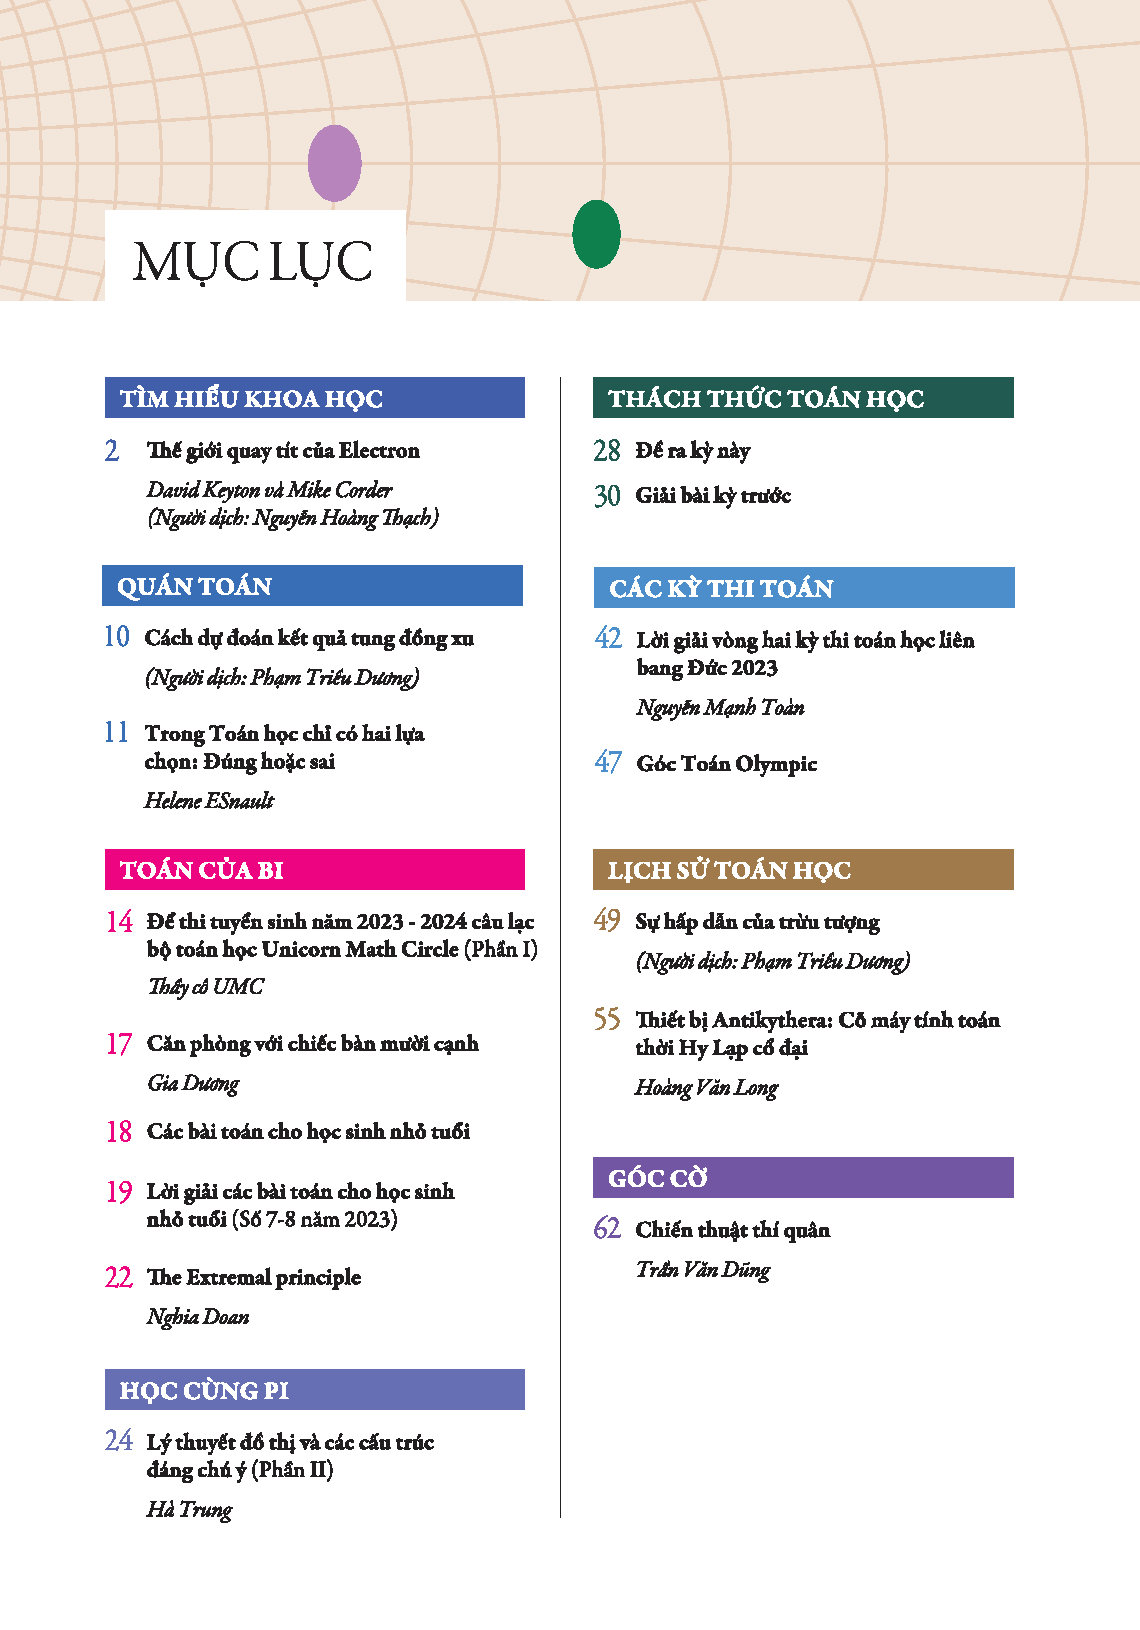
\includegraphics[scale=1]{ML.pdf}}}
	 \centering
	 \vspace*{0cm}
	 \endgroup
	 \newpage	  
	 \pagestyle{empty}

	\setcounter{page}{2}

	\setcounter{figure}{0}
	\thispagestyle{timhieukhoahocnone}
\pagestyle{timhieukhoahoc}
\everymath{\color{timhieukhoahoc}}
\blfootnote{$^1$\text{\color{timhieukhoahoc}https://phys.org/news/2023-10-scientists-nobel-prize-physics-electrons.html}}
\blfootnote{$^2$\text{\color{timhieukhoahoc}Viện Toán học.}}

\graphicspath{{../timhieukhoahoc/pic/}}
\begingroup
\AddToShipoutPicture*{\put(0,616){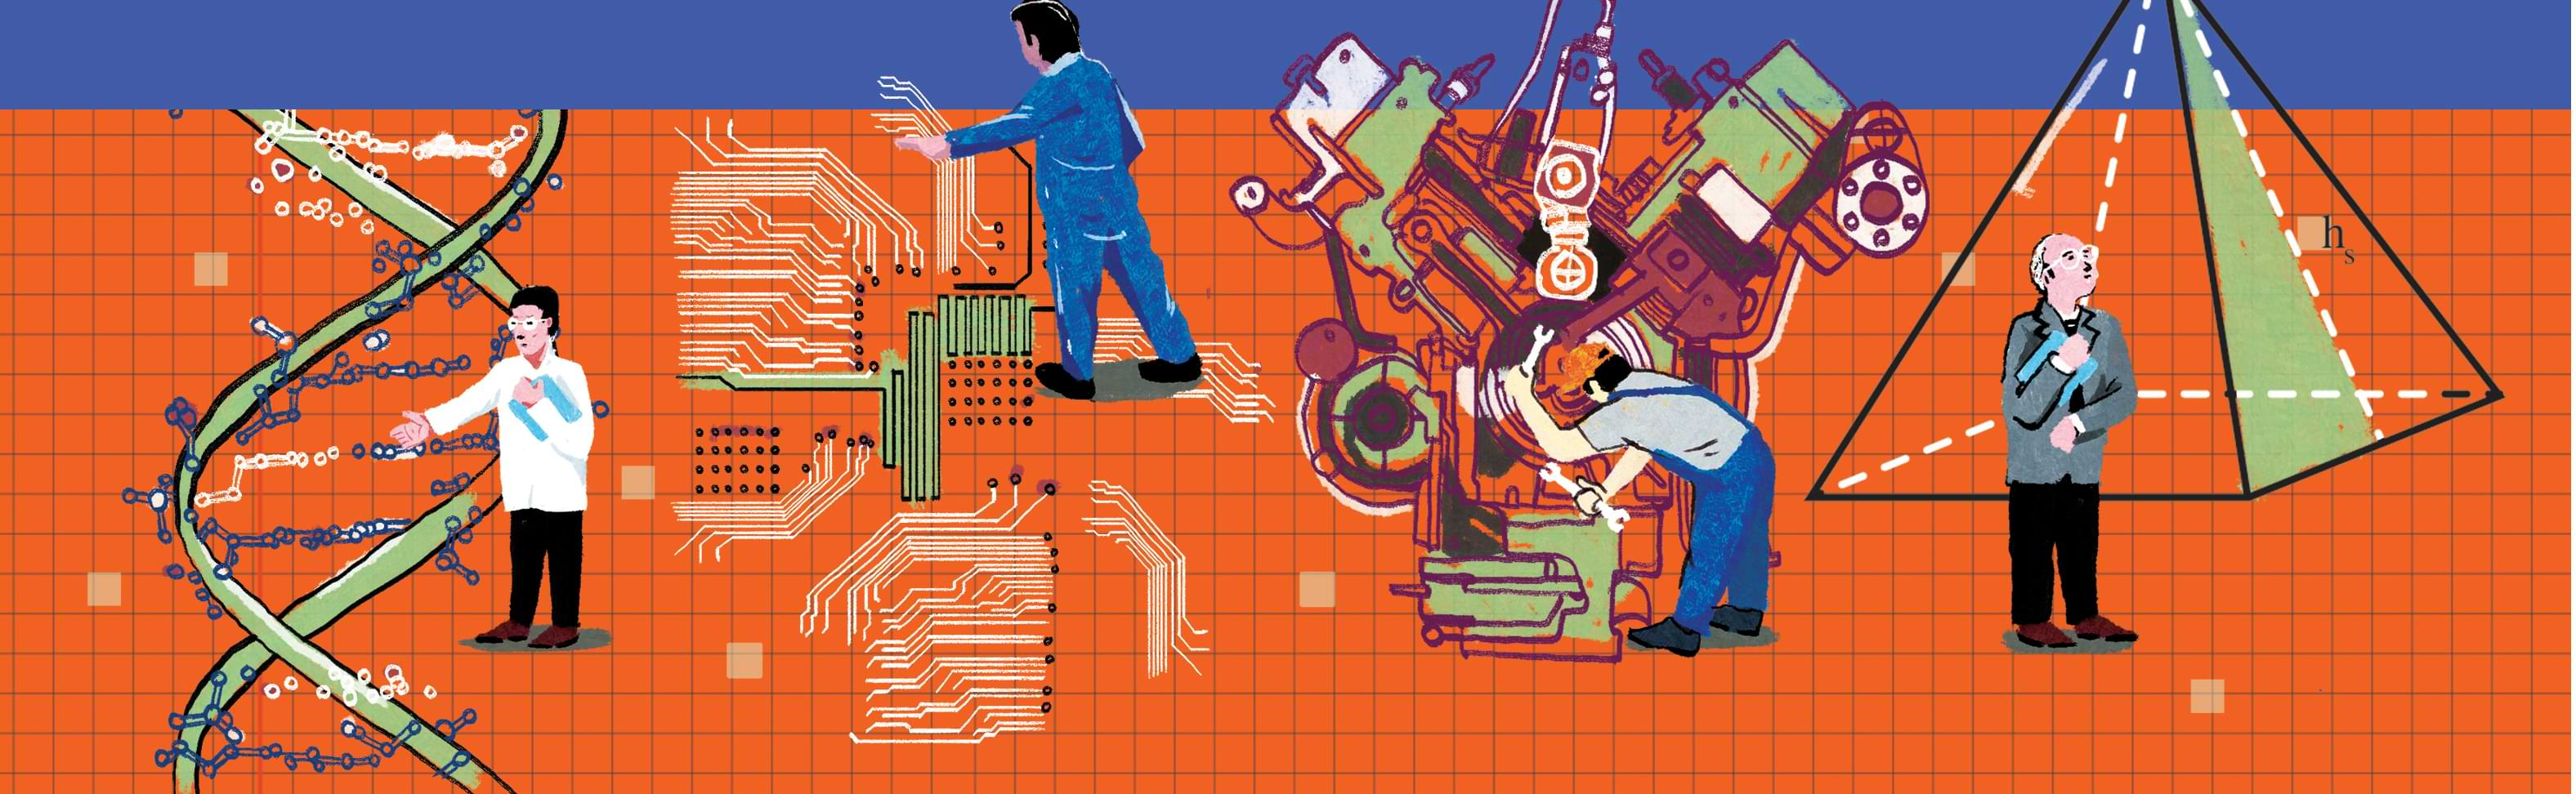
\includegraphics[width=19.3cm]{../bannertimhieu}}}
\AddToShipoutPicture*{\put(60,533){
\includegraphics[scale=1]{../tieude.pdf}}}
\centering
\endgroup
\vspace*{170pt}

\begin{multicols}{2}
	Hôm thứ ba ngày $3$ tháng $10$ vừa qua, ba nhà khoa học đã giành được Giải Nobel Vật lý $2023$ nhờ mang đến cho chúng ta cái nhìn đầu tiên về thế giới siêu tốc độ của các electron quay tít, một lĩnh vực có thể sẽ giúp cải tiến các thiết bị điện tử hoặc chẩn đoán bệnh.
	\begin{figure}[H]
		\vspace*{-5pt}
		\centering
		\captionsetup{labelformat= empty, justification=centering}
		
\includegraphics[width= 1\linewidth]{1}
		\caption{\small\textit{\color{timhieukhoahoc}Ảnh: Viện Hàn lâm Khoa học Hoàng gia Thụy~Điển.}}
		\vspace*{-10pt}
	\end{figure}
	Giải thưởng được trao cho nhà vật lý Pháp -- Thụy Điển Anne L'Huillier, nhà vật lý người Pháp Pierre Agostini và nhà vật lý gốc Hungary Ferenc Krausz, vì công trình của họ về thành phần tí hon chạy quanh hạt nhân của nguyên tử và là cái cơ bản của hầu như mọi thứ: hóa học, vật lý, cơ thể và vật dụng của chúng ta.
	\vskip 0.1cm
	Theo các chuyên gia, electron di chuyển nhanh đến nỗi con người không thể cô lập được chúng, nhưng bằng cách quan sát trong những tích tắc nhỏ nhất có thể, các nhà khoa học hiện đã có cái nhìn thoáng qua ``mờ mờ" về chúng, qua đó mở ra nhiều ngành khoa học hoàn toàn mới.
	\vskip 0.1cm
	``Electron di chuyển rất nhanh, và chúng thực sự là lực lượng lao động ở mọi nơi," Mats Larsson, thành viên Ủy ban Giải thưởng Nobel, cho biết. ``Một khi có thể điều khiển và hiểu được electron, bạn đã tiến được một bước lớn."
	\vskip 0.1cm
	L'Huillier, giáo sư tại Đại học Lund, Thụy Điển, là người phụ nữ thứ năm được Nobel Vật lý.
	\vskip 0.1cm
	``Gửi đến tất cả phụ nữ, tôi muốn nói rằng nếu bạn thích, nếu bạn có một chút đam mê với những thách thức kiểu này, hãy theo đuổi nó," bà nói với hãng tin AP.
	\vskip 0.1cm
	\textbf{\color{timhieukhoahoc}Khám phá được trao Giải Nobel Vật lý}
	\vskip 0.1cm
	Ba nhà khoa học, độc lập với nhau, đã sử dụng xung laser ngày càng nhanh để bắt lại hoạt động của nguyên tử xảy ra ở tốc độ chóng mặt -- một phần tỷ tỷ giây, hay một \textit{atto} giây\footnote[3]{\color{timhieukhoahoc}$1$ atto giây = $10^{-18}$ giây -- Pi.} -- giống như cách các nhiếp ảnh gia sửa dụng cửa trập tốc độ cao để chụp ảnh chim ruồi đang hút mật hoa.
	\begin{figure}[H]
		\vspace*{5pt}
		\centering
		\captionsetup{labelformat= empty, justification=centering}
		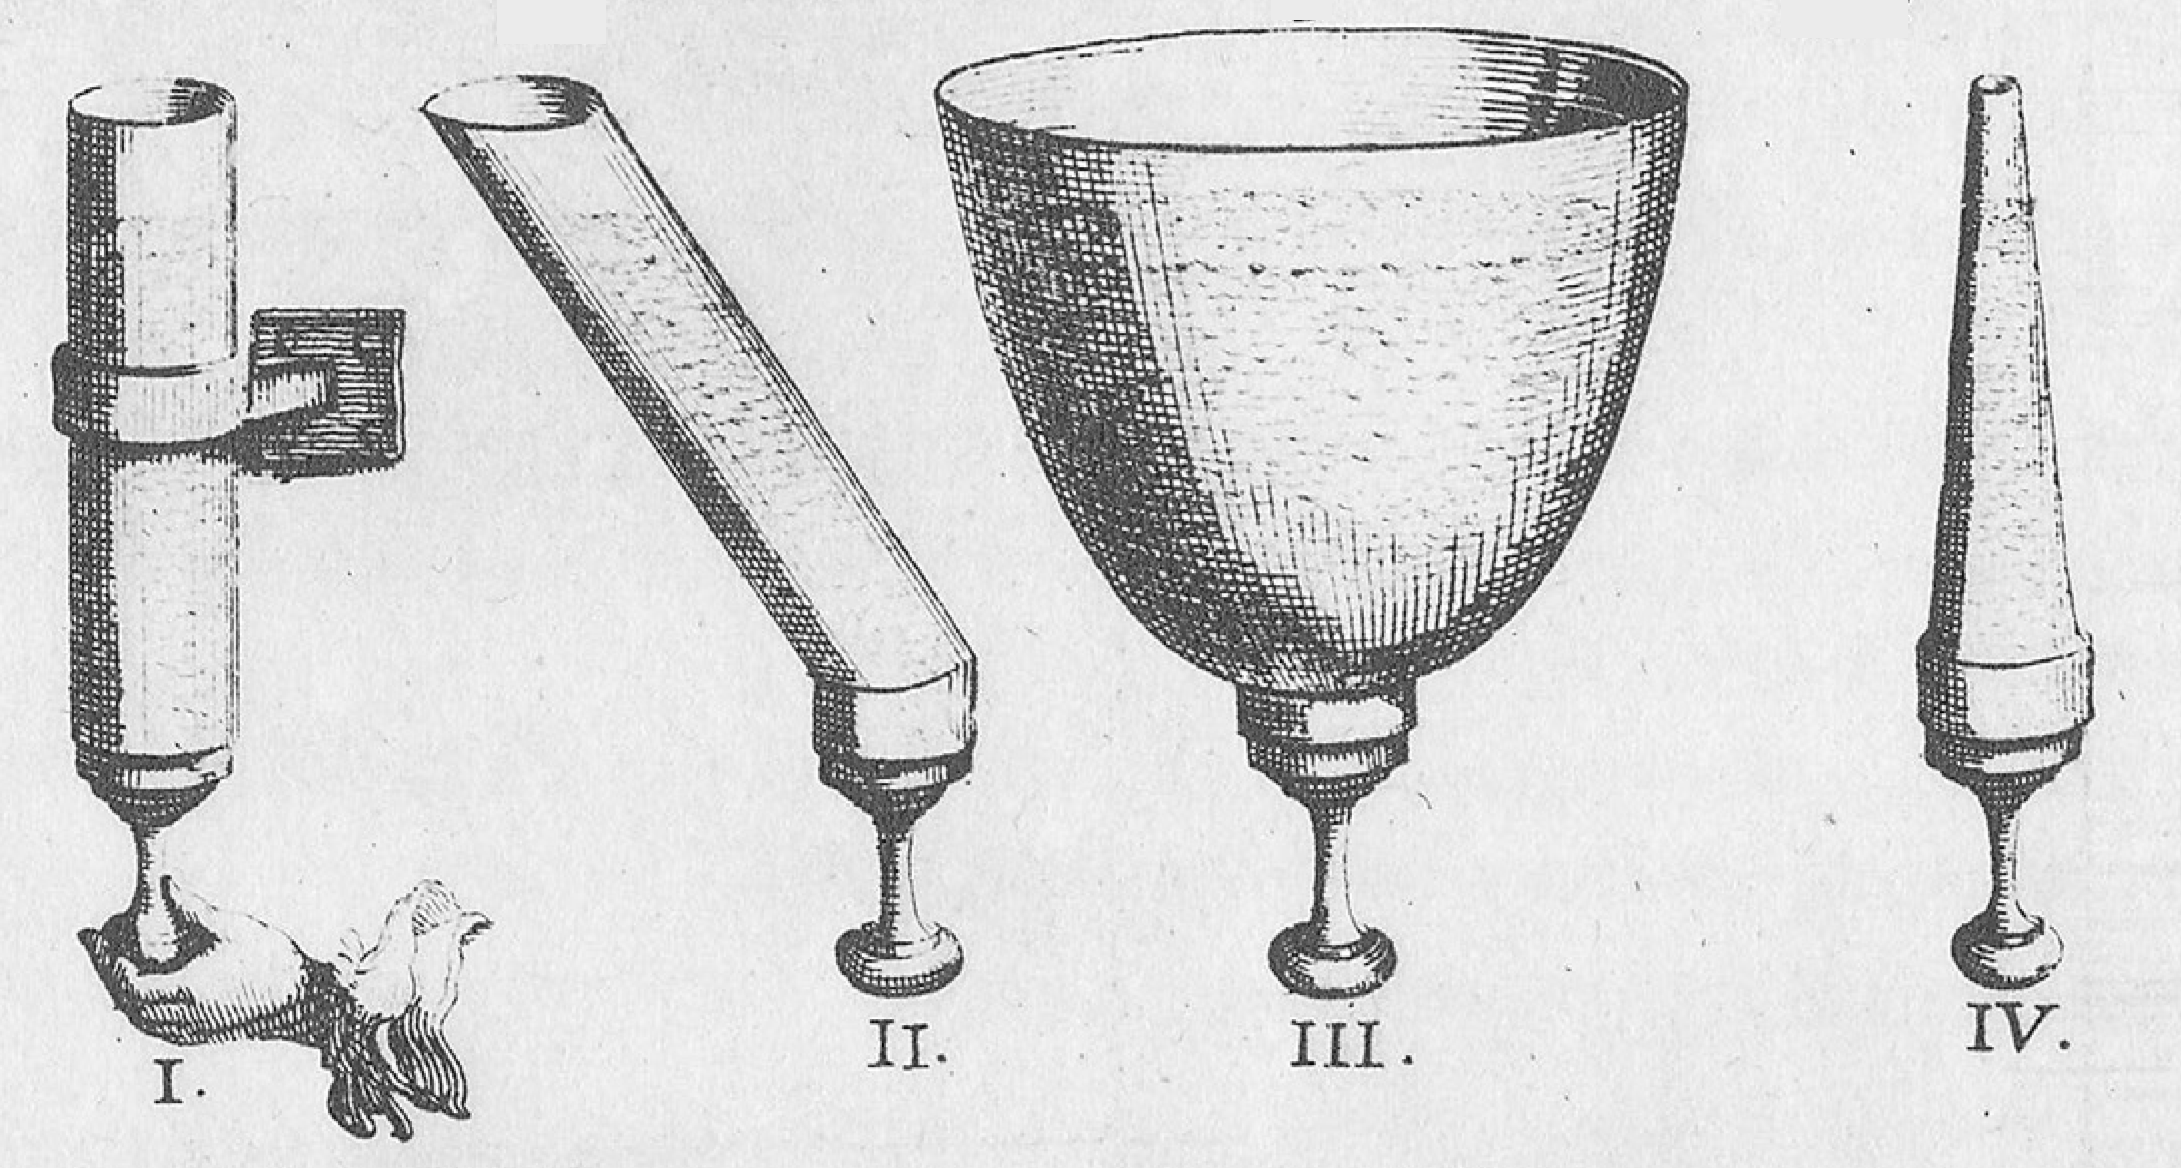
\includegraphics[width= 1\linewidth]{3}
		\caption{\small\textit{\color{timhieukhoahoc}Nhà vật lý Pháp--Thụy Điển Anne L'Huillier}}
		\vspace*{-10pt}
	\end{figure}
	Khoảng thời gian đó ngắn đến mức nào?
	\vskip 0.1cm
	``Hãy lấy một giây, là khoảng thời gian của một nhịp tim," chủ tịch Ủy ban Giải thưởng Nobel, Eva Olsson nói. Để đạt đến cỡ atto giây, cần chia nó cho $1000$ sáu lần.
	\vskip 0.1cm
	Nhà vật lý Mark Pearce, thành viên Ủy ban Giải thưởng Nobel, nói rằng ``số atto giây trong một giây bằng số giây đã trôi qua kể từ Big Bang, khoảng $13{,}8$ tỷ năm trước."
	\vskip 0.1cm
	Nhưng ngay cả khi ``thấy" được electron, các nhà khoa học cũng không thấy được hết.
	\vskip 0.1cm
	``Bạn có thể thấy nó ở phía bên này hay phía bên kia của một phân tử," L'Huillier, năm nay $65$ tuổi, nói. ``Nó vẫn rất mờ."
	\vskip 0.1cm
	``Electron giống sóng, như sóng trên mặt nước, nhiều hơn là giống hạt, và cái chúng tôi đo với kỹ thuật của mình là vị trí của ngọn sóng," bà nói thêm.
	\vskip 0.1cm
	\textbf{\color{timhieukhoahoc}Vì sao electron quan trọng?}
	\vskip 0.1cm
	Electron có vai trò then chốt vì chúng chính là ``cách các nguyên tử liên kết với nhau," L'Huillier nói. Đó là nơi diễn ra các phản ứng hóa học.
	\vskip 0.1cm
	``Dù ta không thể thấy chúng, electron hiện diện khắp mọi nơi trong cuộc sống của chúng ta, theo cả nghĩa cuộc sống sinh học lẫn cuộc sống kỹ thuật, cuộc sống hàng ngày," Krausz nói tại một buổi họp báo. ``Trong cuộc sống sinh học, electron tạo nên chất keo giữa các nguyên tử, từ đó các nguyên tử tạo thành phân tử, và các phân tử này là những viên gạch nhỏ nhất để xây dựng nên mọi cơ thể sống."
	\vskip 0.1cm
	Và nếu muốn hiểu cách chúng làm việc, bạn cần biết cách chúng di chuyển, Krausz nói.
	\vskip 0.1cm
	Hiện tại, khoa học này phục vụ cho việc tìm hiểu vũ trụ của chúng ta, nhưng người ta hy vọng nó cuối cùng sẽ có ứng dụng thực tế trong điện tử, chẩn đoán bệnh và hóa học cơ bản.
	\vskip 0.1cm
	L'Huillier nói rằng công trình của bà cho thấy tầm quan trọng của việc tiến hành nghiên cứu cơ bản mà không cần biết có ứng dụng trong tương lai hay không: bà đã làm việc với nó $30$ năm trước khi những ứng dụng thực tế trở nên rõ ràng hơn.
	\begin{figure}[H]
		\vspace*{-5pt}
		\centering
		\captionsetup{labelformat= empty, justification=centering}
		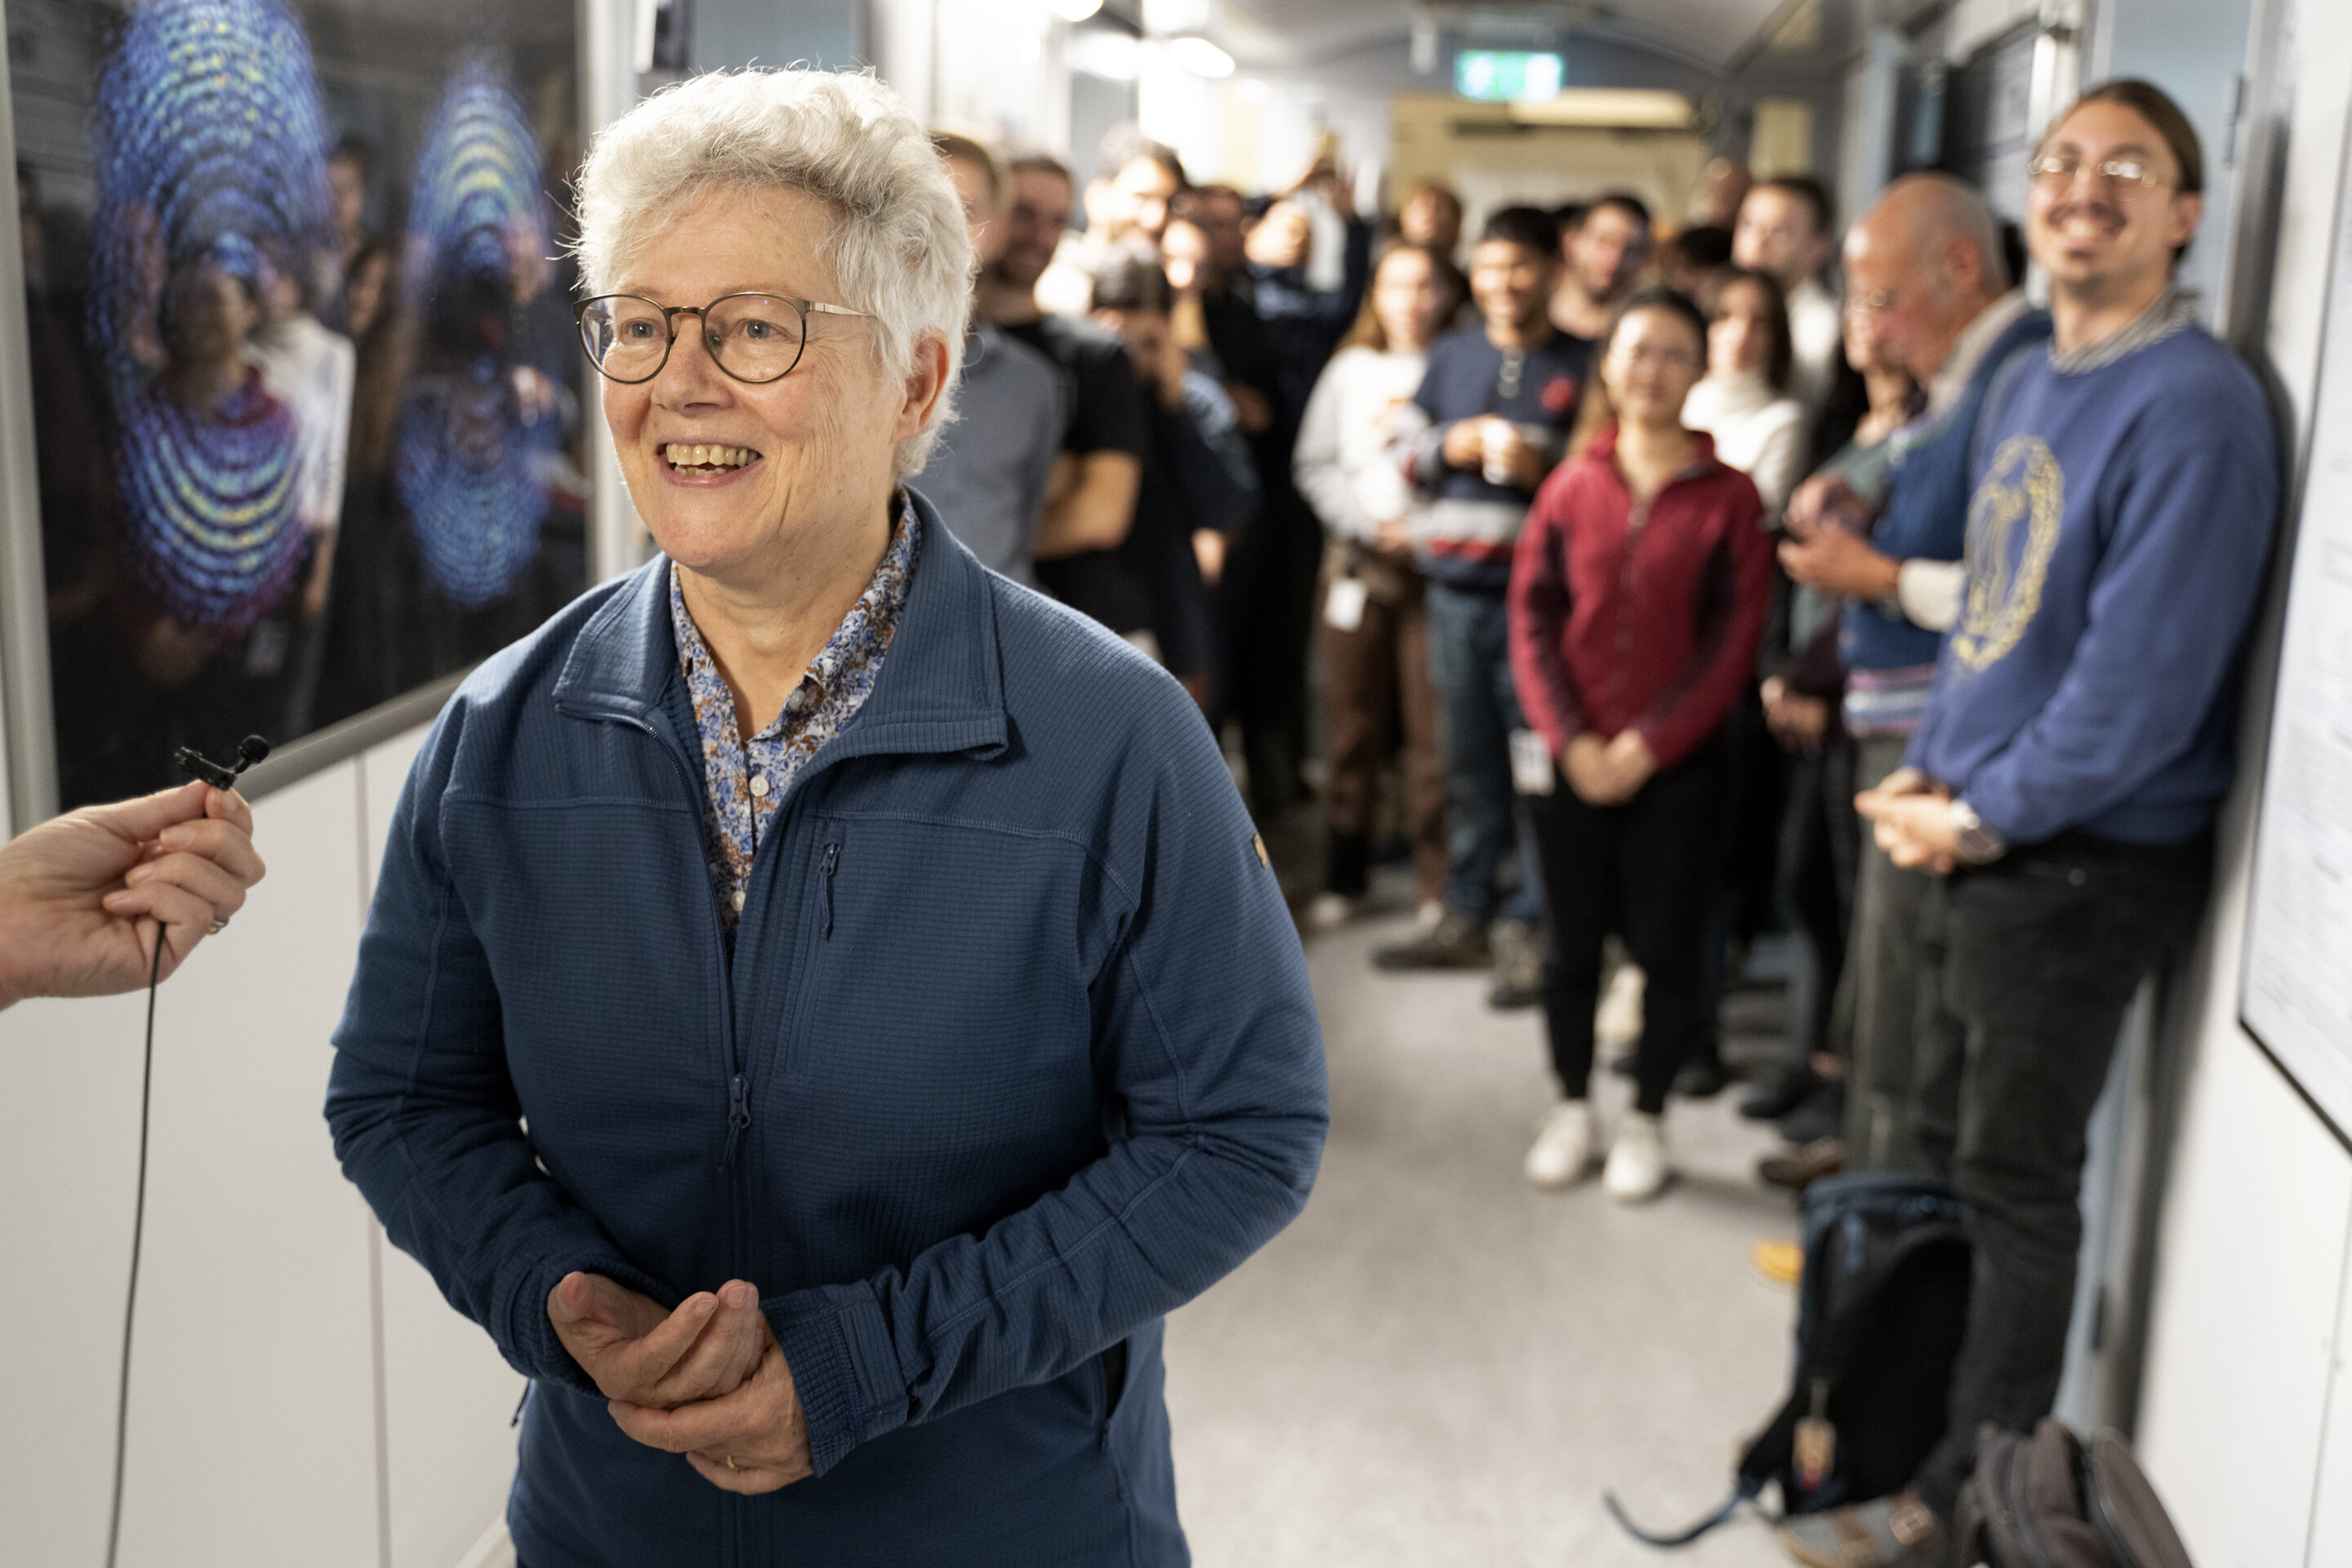
\includegraphics[width= 1\linewidth]{2}
		\caption{\small\textit{\color{timhieukhoahoc}Anne L'Huillier trả lời phỏng vấn tại Đại học Lund, Lund, Thụy Điển hôm thứ ba $3/10/2023$.}}
		\vspace*{-10pt}
	\end{figure}
%	\end{figure}
%	\begin{figure}[H]
%		\vspace*{-5pt}
%		\centering
%		\captionsetup{labelformat= empty, justification=centering}
%		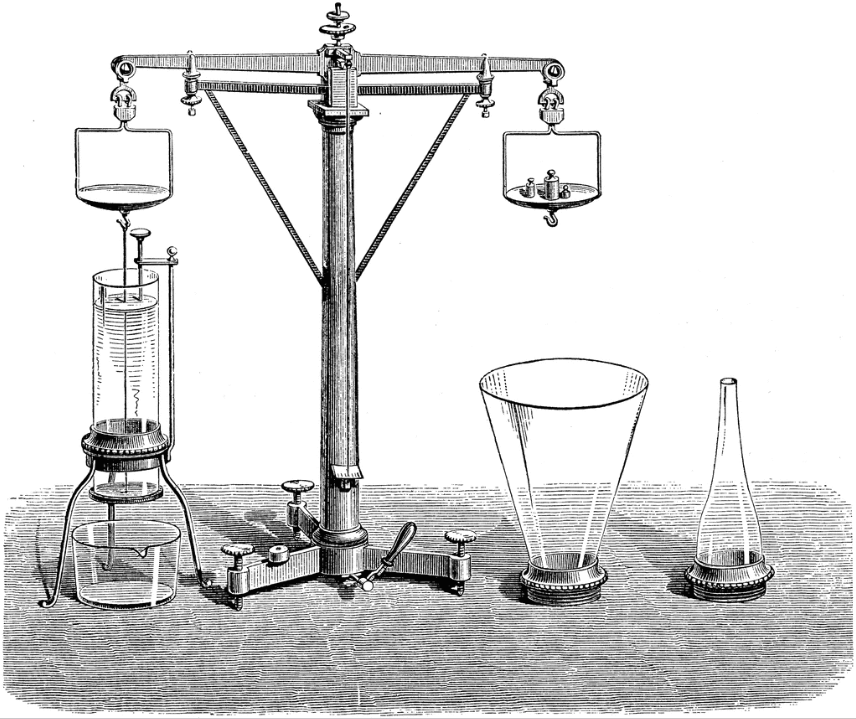
\includegraphics[width= 1\linewidth]{4}
%		%		\caption{\small\textit{\color{}}}
%		\vspace*{-15pt}
%	\end{figure}
	\textbf{\color{timhieukhoahoc}Phản ứng của ba nhà khoa học}
	\vskip 0.1cm
	Khi nhận được cuộc gọi báo tin được giải thưởng, L'Huillier đang dạy vật lý cơ bản dành cho kỹ sư cho khoảng $100$ sinh viên tại Lund; điện thoại của bà để ở chế độ im lặng và bà không nghe máy. Bà kiểm tra điện thoại trong giờ giải lao và gọi lại cho Ủy ban Giải thưởng Nobel.
	\vskip 0.1cm
	Sau đó bà quay lại dạy tiếp.
	\vskip 0.1cm
	``Lúc ấy tôi đang rất tập trung, tôi quên đi Giải Nobel và cố kết thúc bài giảng của mình," bà nói với AP. Bà kết thúc bài giảng sớm một chút để có thể trả lời họp báo công bố giải thưởng tại Viện Hàn lâm Khoa học Hoàng gia Thụy Điển ở Stockholm.
	\vskip 0.1cm
	``Đây là giải thưởng cao quý nhất và tôi thật hạnh phúc được nhận nó. Thật không thể tin được," bà nói ở buổi họp báo. ``Các bạn biết đấy, không có nhiều phụ nữ được giải này, bởi thế nó rất đặc biệt."
	\vskip 0.1cm
	Ban tổ chức giải Nobel đăng trên tài khoản mạng xã hội của mình một bức ảnh L'Huillier đang nghe điện thoại.
	\begin{figure}[H]
		\vspace*{-5pt}
		\centering
		\captionsetup{labelformat= empty, justification=centering}
		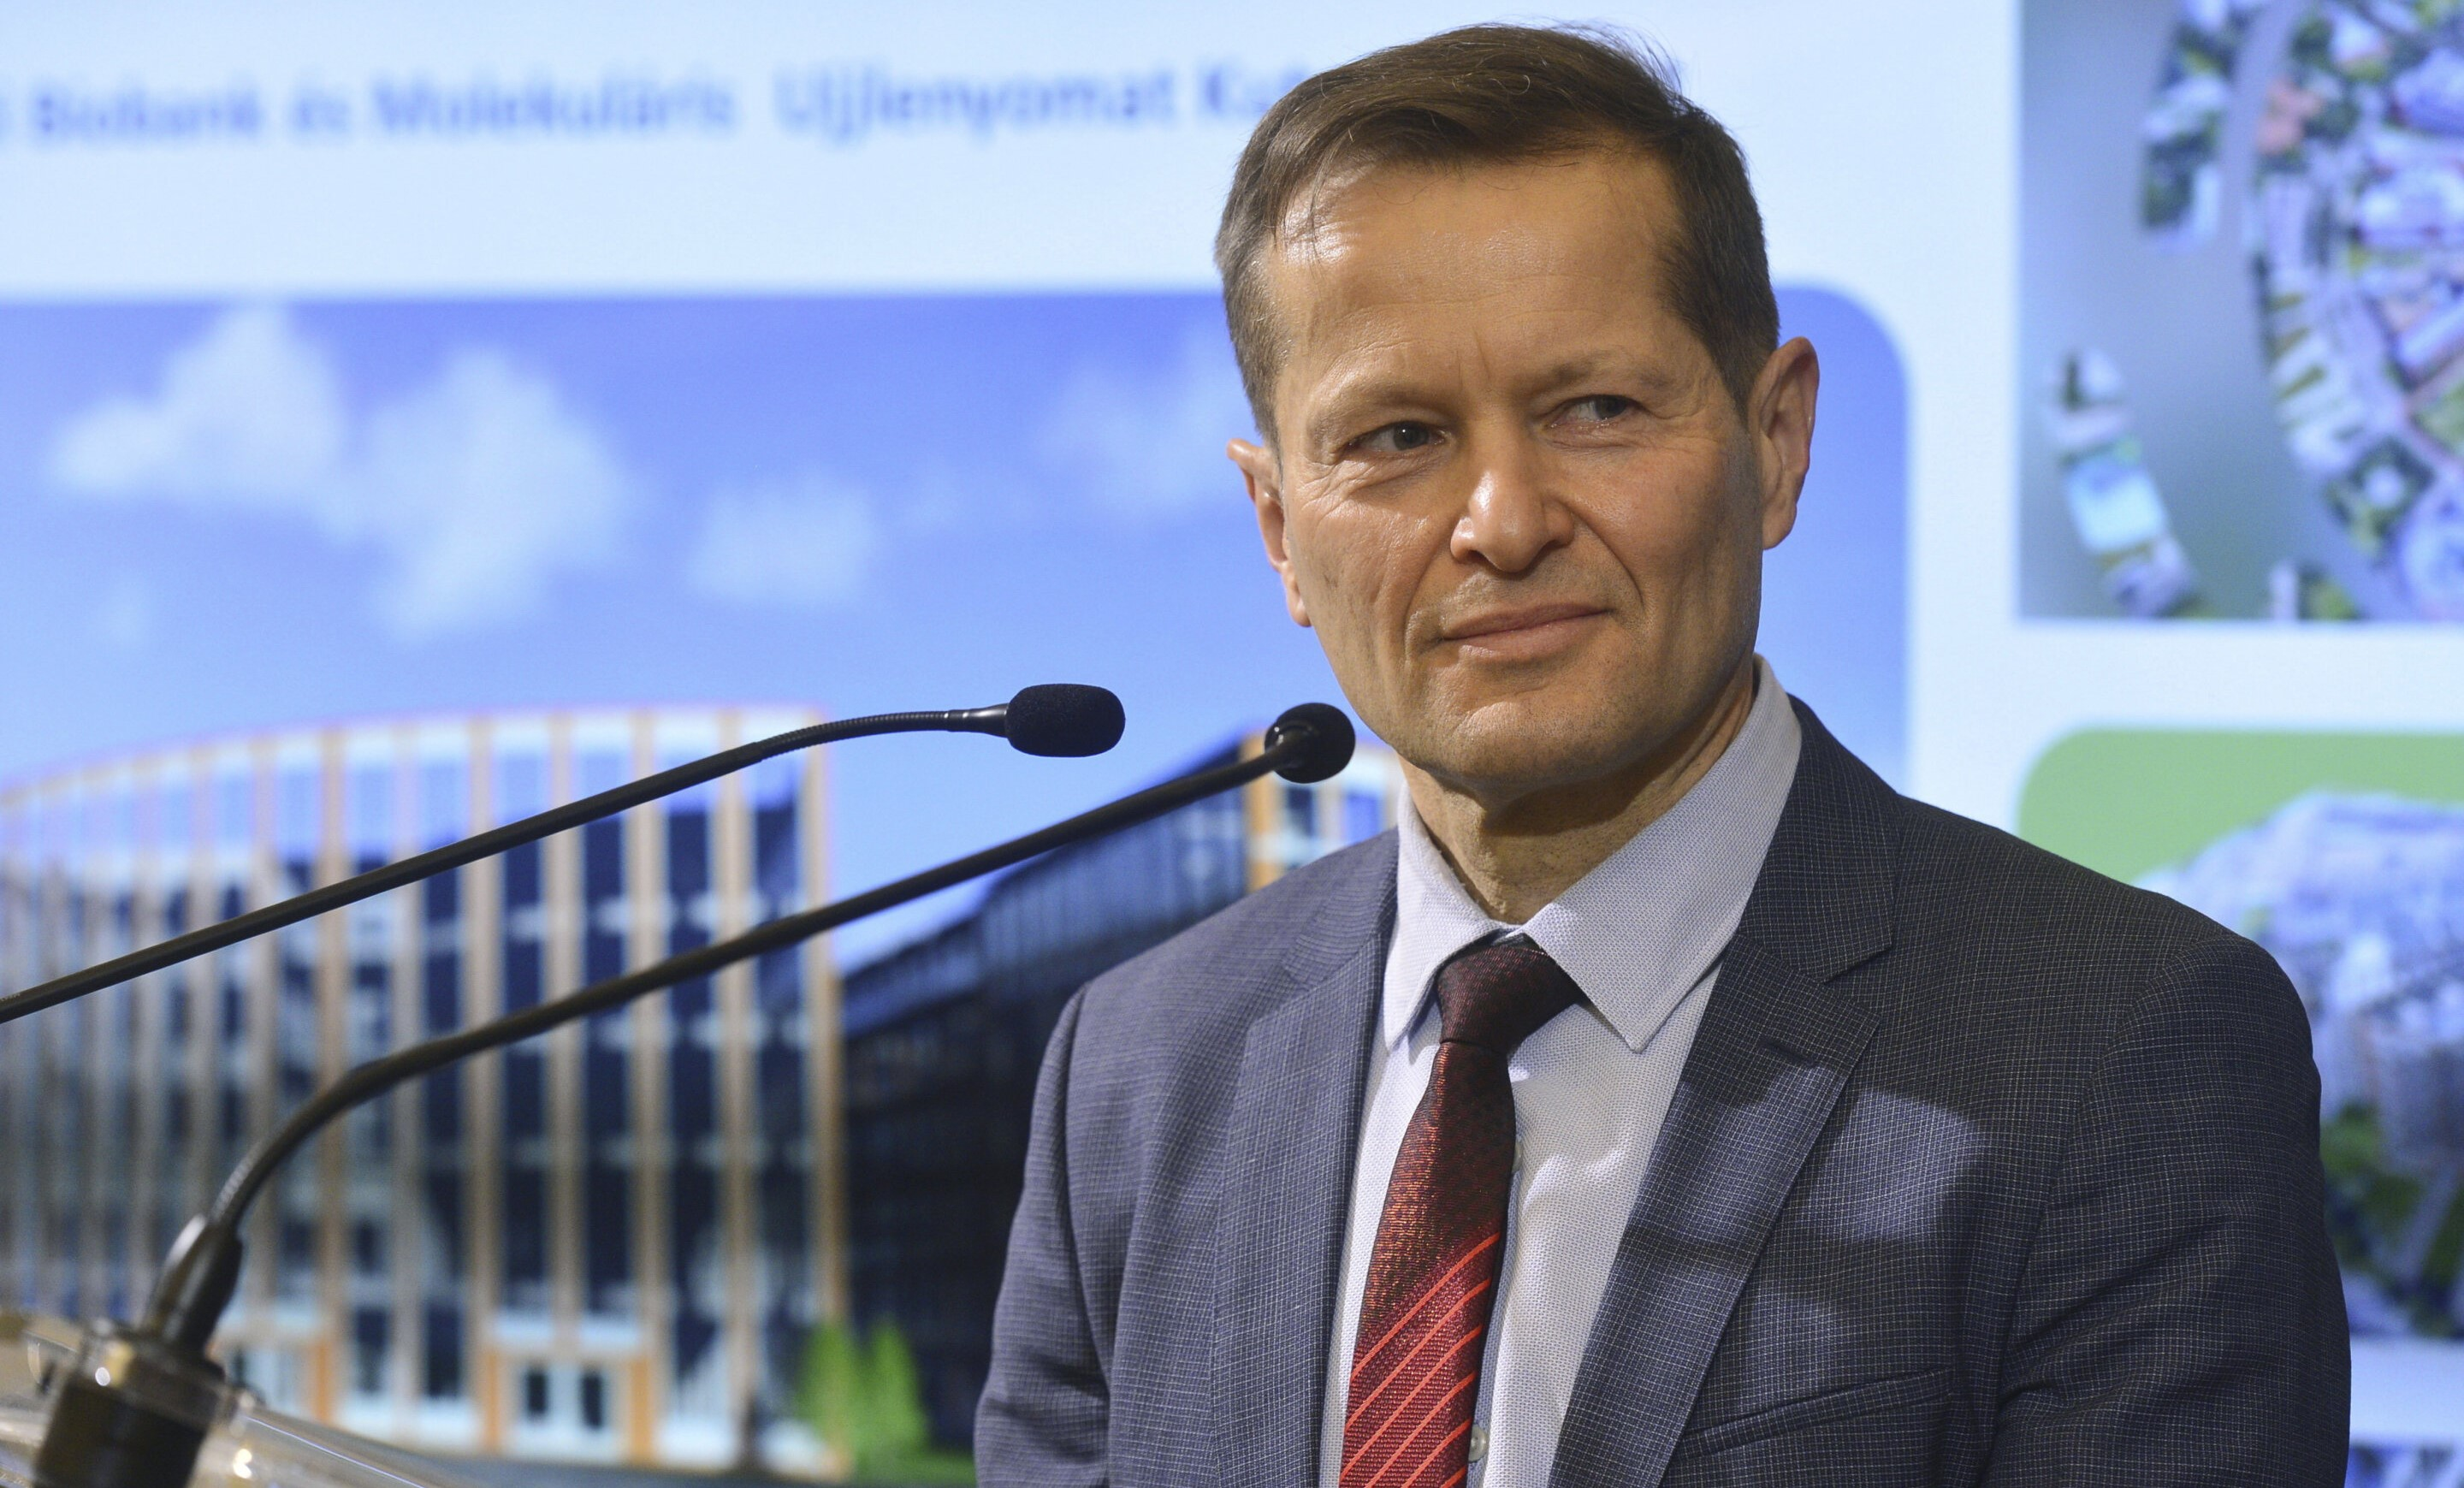
\includegraphics[width= 1\linewidth]{7}
		\caption{\small\textit{\color{timhieukhoahoc}Nhà vật lý người Hungary Ferenc Krausz.}}
		\vspace*{-10pt}
	\end{figure}
	``Cảnh báo: nhà giáo tận tâm!" bài đăng trên Twitter, nay là X, viết. ``Đến cả giải Nobel Vật lý $2023$ cũng không thể kéo Anne L'Huillier khỏi sinh viên của bà."
	\vskip 0.1cm
	Và L'Huillier cho biết khi đó vẫn phải giữ bí mật về giải thưởng nên bà không được phép giải thích với sinh viên, nhưng họ đoán được.
	\vskip 0.1cm
	Agostini, giáo sư danh dự tại Đại học Bang Ohio, khi đó đang ở Paris; Ủy ban Giải thưởng Nobel không liên lạc được với ông trước khi công bố việc ông được giải với cả thế giới.
	\vskip 0.1cm
	``Tôi không nhận được cuộc gọi nào từ ủy ban giải thưởng. Có lẽ không đúng. Tôi không biết," ông cười khi trả lời AP. ``Tôi nghĩ họ tìm tôi ở Columbus\footnote[4]{\color{timhieukhoahoc}Thủ phủ bang Ohio -- Pi.}."
	\vskip 0.1cm
	``Chắc chắn có nhiều người trẻ hơn đánh giá cao giải thưởng này hơn tôi," vị giáo sư $82$ tuổi nói đùa. ``Nó cũng tốt đấy, nhưng với tôi thì hơi muộn."
	\vskip 0.1cm
	Nhưng, ông nói thêm: ``Tôi không nghĩ mình sẽ xứng đáng nếu được trao giải sớm hơn!"
	\vskip 0.1cm
	Krausz, thuộc Viện Quang học Lượng tử Max Planck và Đại học Ludwig Maximilian tại Munich, nói với các phóng viên rằng ông bị choáng ngợp.
	\vskip 0.1cm
	``Từ $11$ giờ sáng đến giờ tôi vẫn đang nghĩ xem mình đang ở trong hiện thực hay trong một giấc mơ dài," nhà vật lý $61$ tuổi nói.
	\vskip 0.1cm
	Cuộc gọi từ ủy ban giải thưởng được hiển thị ``không có ID người gọi" và thường thì Krausz không nghe những cuộc gọi như vậy, nhưng lần này, ông ``nghĩ rằng mình sẽ thử nghe, và rõ ràng không thể dập máy ngay."
	\vskip 0.1cm
	Năm ngoái, cùng với nhà khoa học Paul Corkum của Đại học Ottawa, Krausz và L'Huillier được trao giải thưởng vật lý cao quý Wolf vì những công trình của họ. Giải Nobel chỉ được trao cho không quá ba người, và Krausz nói rằng thật đáng tiếc khi nó không thể được trao cho Corkum.
	\vskip 0.1cm
	Corkum là chìa khóa đối với cách đo các xung laser xảy ra trong tích tắc, và điều này mang tính cốt yếu, Krausz nói.
	\begin{figure}[H]
		\vspace*{-5pt}
		\centering
		\captionsetup{labelformat= empty, justification=centering}
		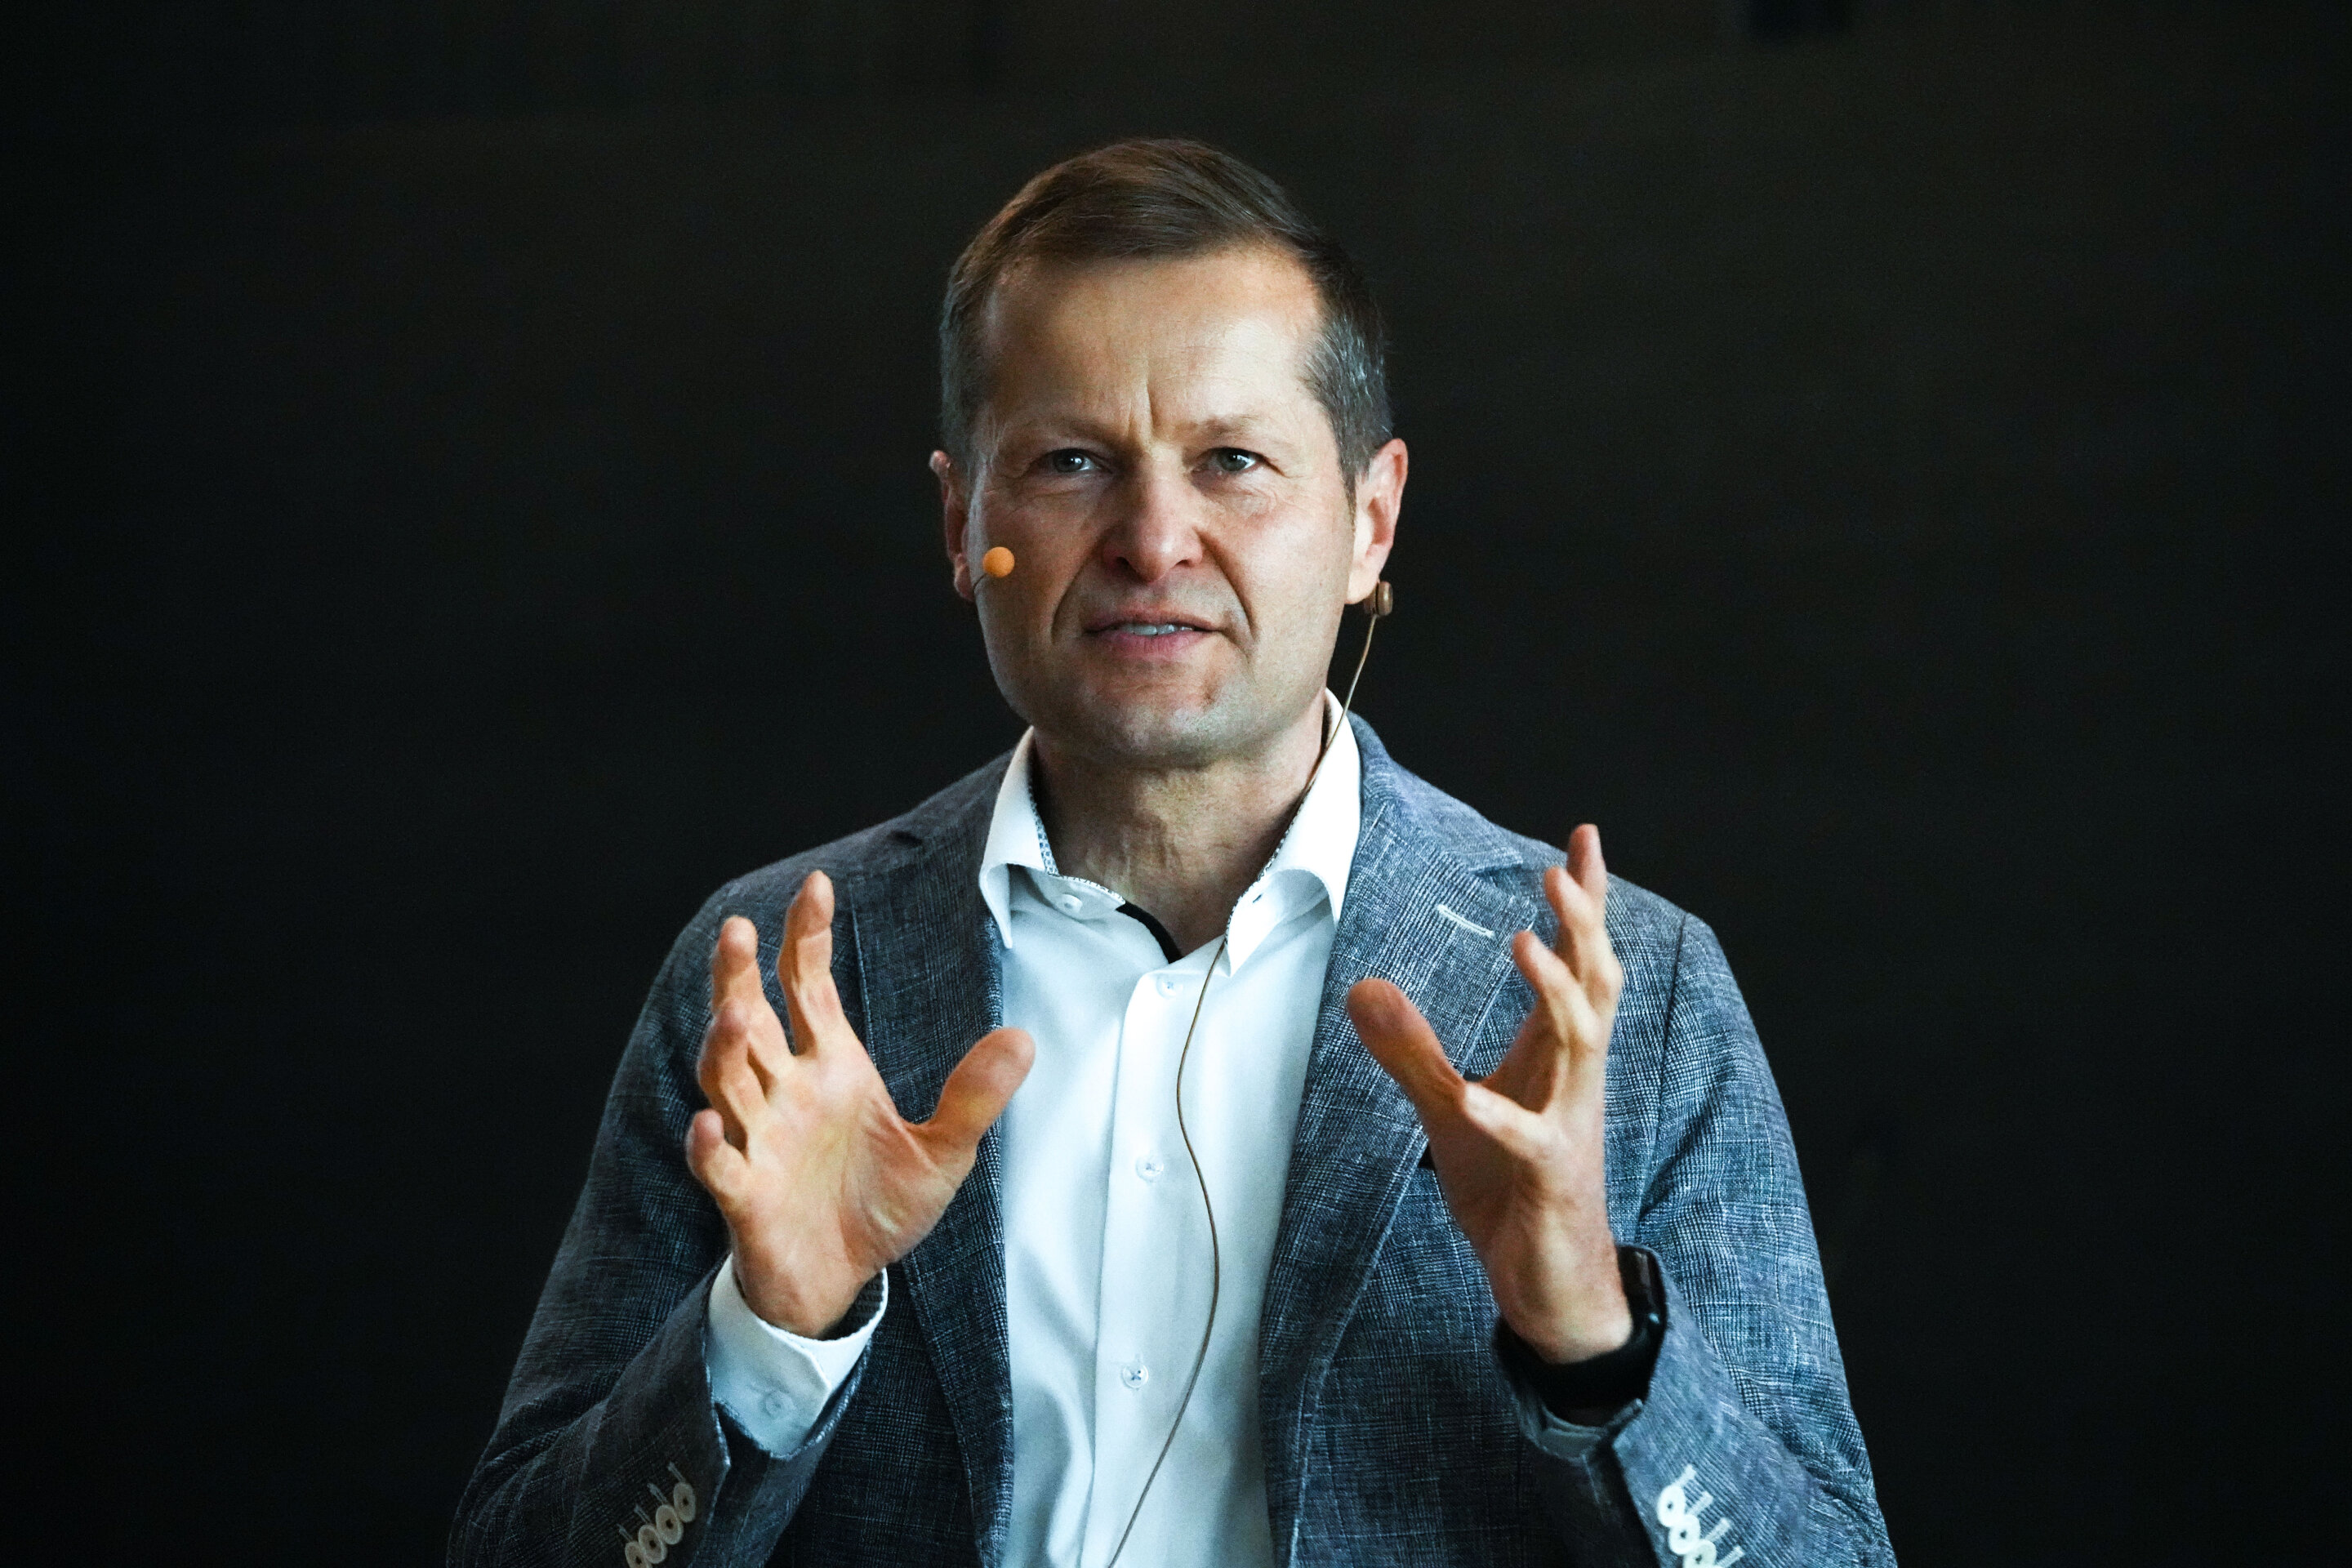
\includegraphics[width= 1\linewidth]{5}
		\caption{\small\textit{\color{timhieukhoahoc}Ferenc Krausz trong một buổi thuyết trình tại Viện Quang học Lượng tử Max Planck, Munich, Đức hôm thứ ba $3/10/2023$.}}
		\vspace*{-15pt}
	\end{figure}
	Giải Nobel có giá trị tiền thưởng khoảng $1$ triệu đô--la Mỹ, được trao theo di chúc của người sáng lập ra nó, nhà phát minh người Thụy Điển Alfred Nobel.
	\vskip 0.1cm
	Giải Nobel Vật lý được công bố hai ngày sau khi hai nhà khoa học được giải Nobel Y học -- Sinh lý học vì những khám phá giúp tạo ra vaccine mRNA cho COVID--$19$.
	\vskip 0.1cm
	\textbf{\color{timhieukhoahoc}Thông báo của Ủy ban Giải thưởng Nobel:}
	\vskip 0.1cm
	Viện Hàn lâm Khoa học Hoàng gia Thụy Điển quyết định trao giải Nobel Vật lý $2023$ cho
	\vskip 0.1cm
	\textbf{\color{timhieukhoahoc}Pierre Agostini}, Đại học Bang Ohio, Columbus, Mỹ
	\vskip 0.1cm
	\textbf{\color{timhieukhoahoc}Ferenc Krausz},  Viện Quang học Lượng tử Max Planck, Garching và Đại học Ludwig Maximilian tại Munich, Đức
	\vskip 0.1cm
	\textbf{\color{timhieukhoahoc}Anne L'Huillier}, Đại học Lund, Thụy Điển
	\vskip 0.1cm
	``vì các phương pháp thực nghiệm tạo ra các xung ánh sáng atto giây nhằm nghiên cứu động lực học của electron trong vật chất".
	\begin{figure}[H]
		\vspace*{-5pt}
		\centering
		\captionsetup{labelformat= empty, justification=centering}
		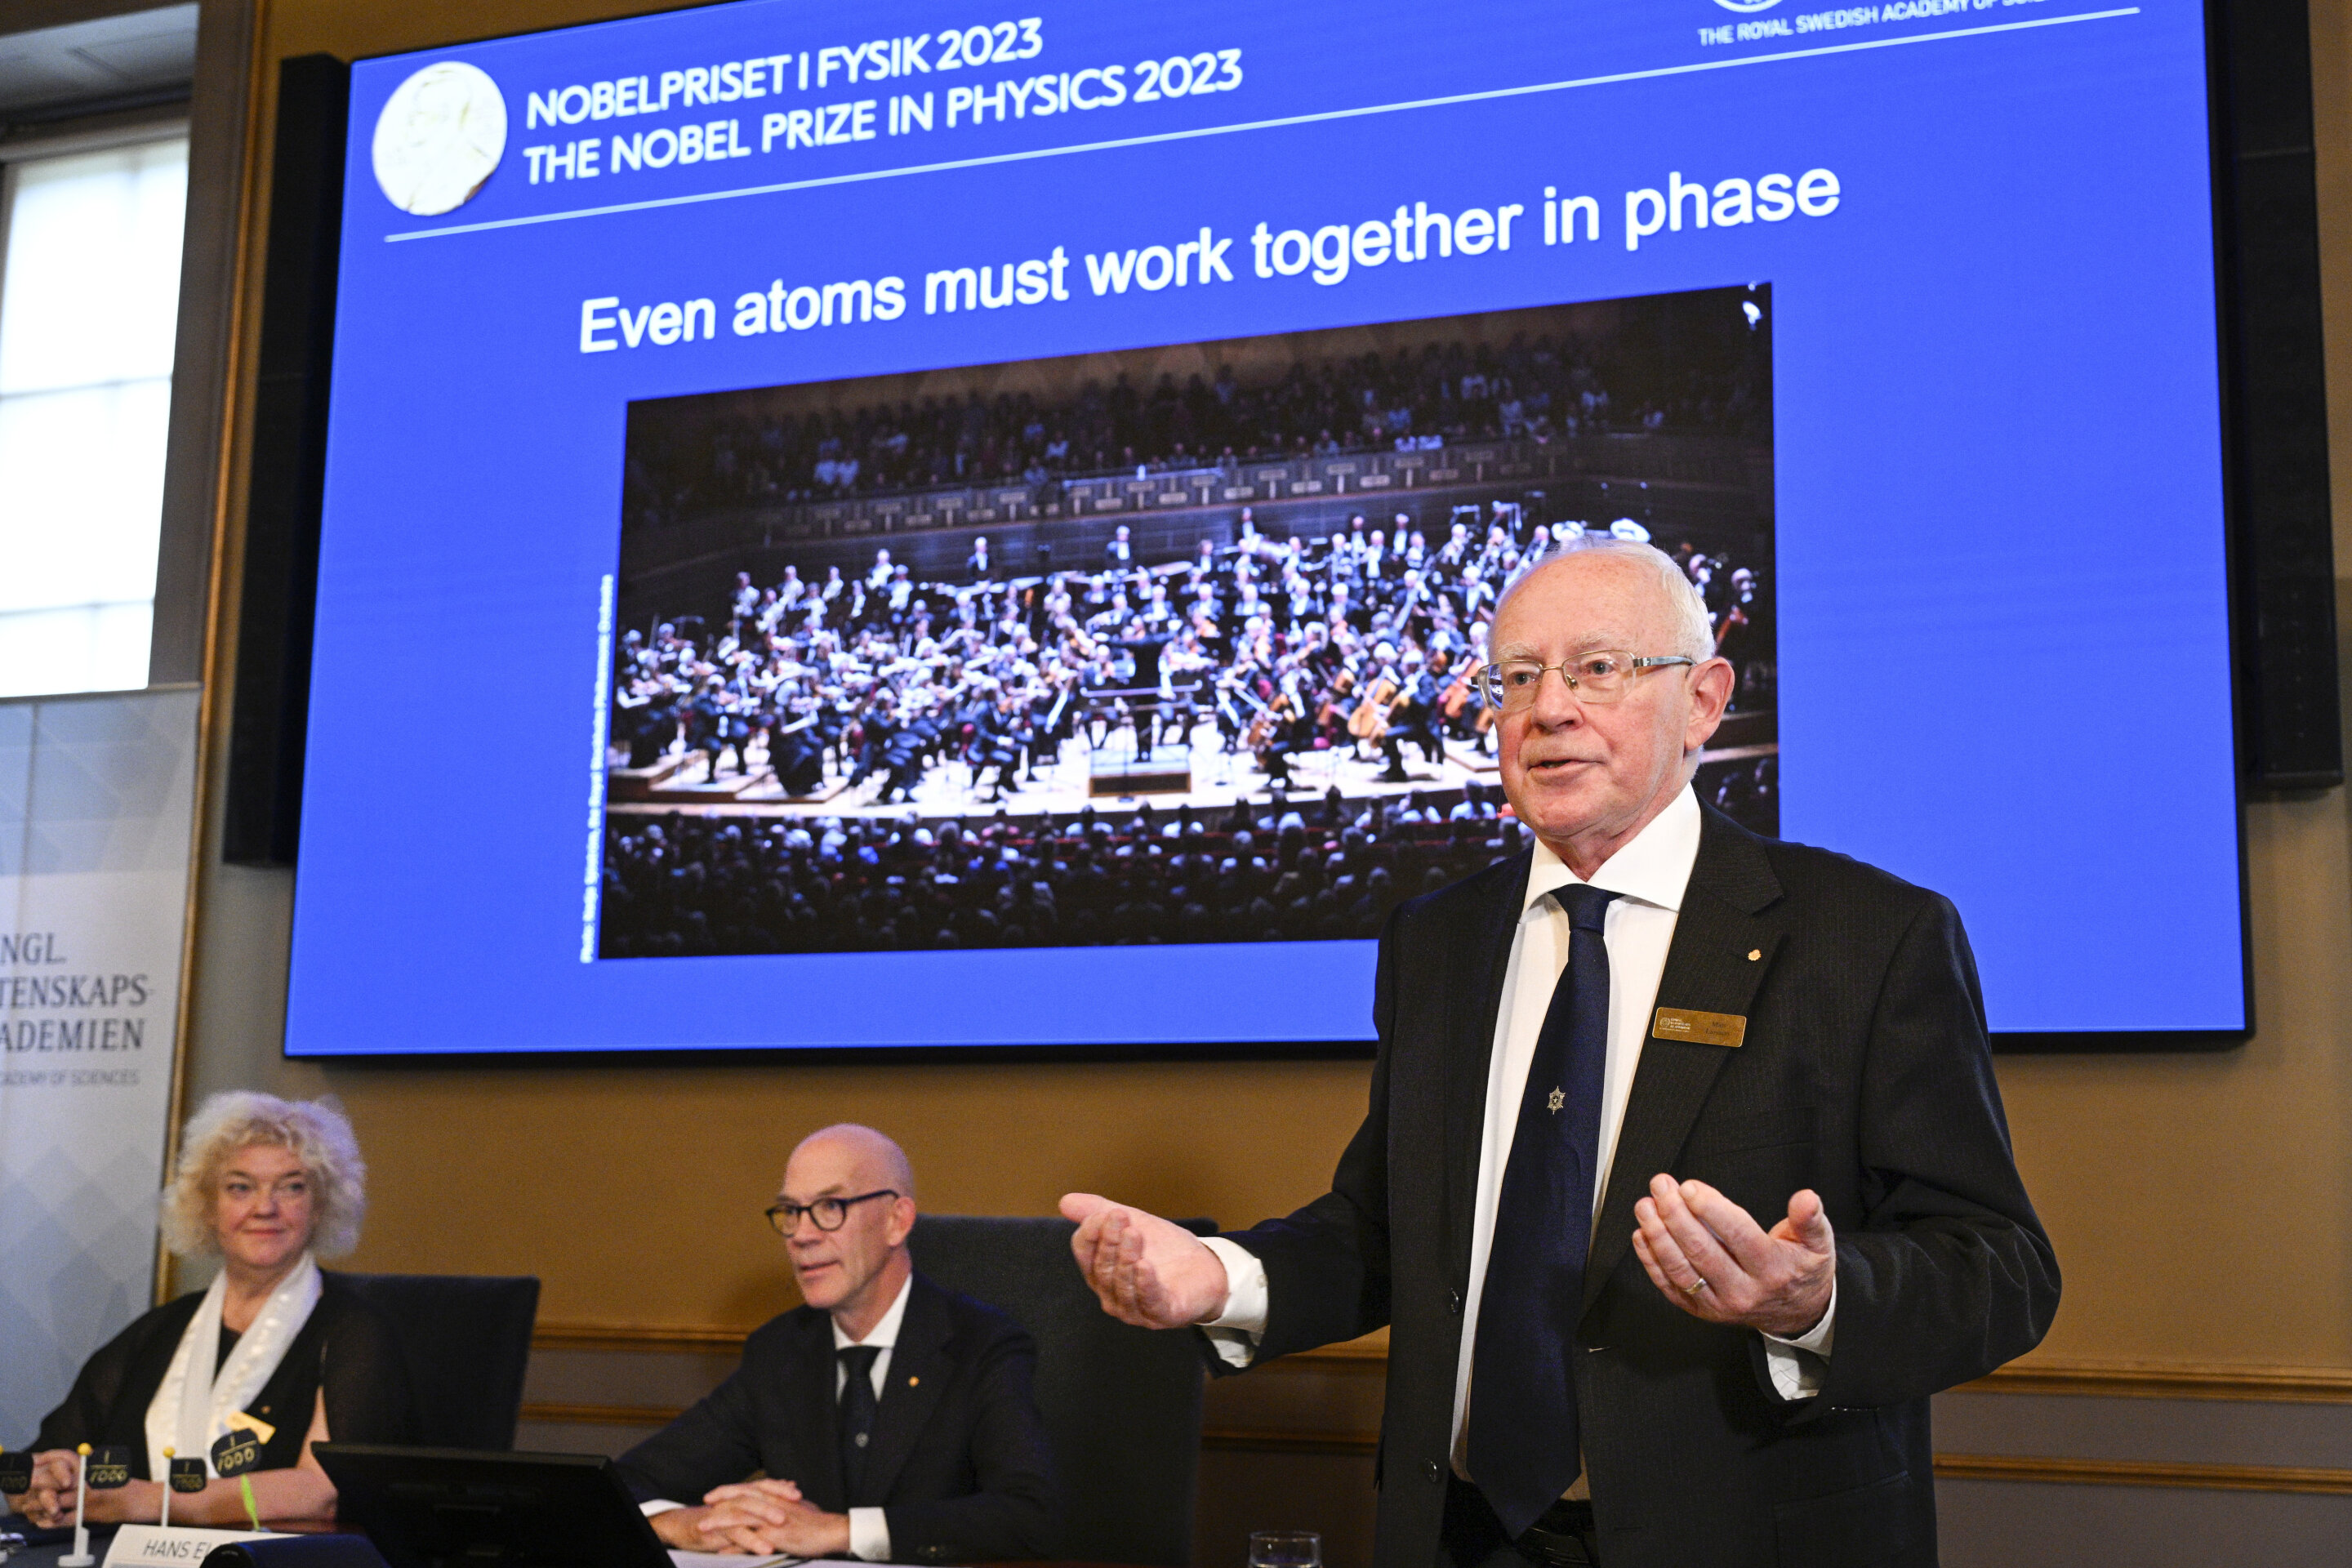
\includegraphics[width= 1\linewidth]{9}
%		\caption{\small\textit{\color{}}}
		\vspace*{-15pt}
	\end{figure}
	\textbf{\color{timhieukhoahoc}Thí nghiệm với ánh sáng bắt được những khoảnh khắc ngắn nhất}
	\vskip 0.1cm
	Ba nhà khoa học được giải Nobel Vật lý $2023$ được vinh danh vì những thí nghiệm cung cấp cho nhân loại những công cụ mới để khám phá thế giới của electron bên trong nguyên tử và phân tử. Pierre Agostini, Ferenc Krausz và Anne L'Huillier đã trình bày một cách tạo ra những xung ánh sáng cực ngắn có thể được dùng để đo các quá trình rất nhanh, trong đó electron di chuyển hoặc thay đổi năng lượng.
	\vskip 0.1cm
	Các sự kiện tốc độ cao chảy vào với nhau khi được quan sát bởi con người, giống như một đoạn phim gồm những hình ảnh tĩnh được nhìn thấy như chuyển động liên tục. Nếu muốn tìm hiểu về những sự kiện thực sự ngắn ngủi, chúng ta cần những công nghệ đặc biệt. Trong thế giới của electron, những thay đổi xảy ra chỉ trong vài chục atto giây -- một atto giây là một khoảng thời gian rất ngắn, ngắn đến nỗi số atto giây trong một giây bằng số giây tính từ khi vũ trụ ra đời.
	\vskip 0.1cm
	Những thí nghiệm của các nhà khoa học được giải đã tạo ra các xung ánh sáng ngắn đến cỡ atto giây, từ đó cho thấy các xung này có thể được sử dụng để cung cấp những hình ảnh về các quá trình bên trong nguyên tử và phân tử.
	\vskip 0.1cm
	Năm $1987$, Anne L'Huillier phát hiện thấy nhiều sóng hài bậc cao khác nhau xuất hiện khi bà truyền laser hồng ngoại qua một khí hiếm. Mỗi sóng hài bậc cao là một sóng ánh sáng mà mỗi chu kỳ của ánh sáng laser bằng một bội của chu kỳ của sóng hài. Chúng được sinh ra do laser tương tác với các phân tử khí; nó cung cấp năng lượng cho một số electron, và năng lượng dư thừa này được phát lại dưới dạng ánh sáng. Anne L'Huillier tiếp tục tìm hiểu hiện tượng này, đặt nền móng cho những đột phá tiếp theo.
	\vskip 0.1cm
	Năm $2001$, Pierre Agostini thành công trong việc tạo ra và nghiên cứu một chuỗi các xung ánh sáng liên tiếp, trong đó mỗi xung chỉ dài $250$ atto giây. Cùng lúc đó, Ferenc Krausz đang tiến hành một loại thí nghiệm khác, cho phép tách riêng một xung ánh sáng dài $650$ atto giây.
	\vskip 0.1cm
	Đóng góp của các nhà khoa học được giải cho phép nghiên cứu các quá trình diễn ra rất nhanh, mà trước đó không thể theo kịp.
	\vskip 0.1cm
	``Giờ chúng ta có thể mở cánh cửa vào thế giới của electron. Vật lý atto giây cho chúng ta cơ hội hiểu được các cơ chế do electron chi phối. Bước tiếp theo sẽ là sử dụng chúng," Eva Olsson, chủ tịch Ủy ban Giải thưởng Nobel về Vật lý, nói.
	\vskip 0.1cm
	Có nhiều ứng dụng tiềm năng trong những lĩnh vực khác nhau. Chẳng hạn, trong điện tử, việc hiểu và điều khiển được hành vi của electron trong vật liệu là rất quan trọng. Các xung atto giây cũng có thể được dùng để nhận dạng các phân tử khác nhau, thí dụ trong chẩn đoán y tế.
	\begin{figure}[H]
		\vspace*{-5pt}
		\centering
		\captionsetup{labelformat= empty, justification=centering}
		
\includegraphics[width= 1\linewidth]{8}
		\caption{\small\textit{\color{timhieukhoahoc}Pierre Agostini, ảnh tại trang web khoa Vật lý, Đại học Bang Ohio.}}
		\vspace*{-10pt}
	\end{figure}
	\textbf{\color{timhieukhoahoc}Electron trong xung ánh sáng}
	\vskip 0.1cm
	Qua các thí nghiệm của mình, ba nhà khoa học được giải năm nay đã tạo được những chớp sáng đủ ngắn để chụp được chuyển động vô cùng nhanh của electron. Anne L'Huillier phát hiện ra một hiệu ứng mới từ tương tác của ánh sáng laser với các nguyên tử khí. Pierre Agostini và Ferenc Krausz cho thấy hiệu ứng này có thể được dùng để tạo ra những xung ánh sáng ngắn hơn những cái có thể được tạo ra trước đó.
	\vskip 0.1cm
	Một con chim ruồi có thể đập cánh $80$ lần mỗi giây. Chúng ta chỉ có thể nhận thấy tiếng vù vù và chuyển động mờ mờ. Với giác quan của con người, chuyển động nhanh bị mờ vào với nhau, và những sự kiện cực ngắn là không thể quan sát. Chúng ta cần đến những biện pháp công nghệ để chụp hoặc mô tả được những khoảnh khắc rất ngắn đó.
	\vskip 0.1cm
	Kỹ thuật chụp ảnh tốc độ cao và ánh sáng nhấp nháy cho phép chụp được hình ảnh chi tiết của những hiện tượng thoáng qua. Một bức ảnh rõ nét chụp một con chim ruồi đang bay đòi hỏi thời gian phơi sáng ngắn hơn nhiều so với một nhịp đập cánh của nó.
	\vskip 0.1cm
	Sự kiện càng nhanh, thời gian chụp ảnh phải càng ngắn để chụp được đúng khoảnh khắc.
	\vskip 0.1cm
	Nguyên lý tương tự được áp dụng cho tất cả các phương pháp để đo hoặc mô tả các quá trình nhanh; mọi phép đo phải được thực hiện nhanh hơn khoảng thời gian để hệ thống được quan sát trải qua một thay đổi nhận biết được, bằng không kết quả sẽ không rõ. Các nhà khoa học được giải năm nay đã tiến hành các thí nghiệm chỉ ra một phương pháp tạo ra các xung ánh sáng đủ ngắn để chụp được hình ảnh về các quá trình bên trong nguyên tử và phân tử.
	\vskip 0.1cm
	Thang thời gian tự nhiên của nguyên tử là cực kỳ nhỏ. Trong một phân tử, các nguyên tử có thể di chuyển và quay trong một phần triệu tỷ giây, hay femto giây\footnote[5]{\color{timhieukhoahoc}$1$ femto giây $= 10^{-15}$ giây -- Pi.} . Những chuyển động này có thể được nghiên cứu với những xung ngắn nhất mà một tia laser có thể tạo ra -- tuy nhiên, khi cả nguyên tử di chuyển, thang thời gian được xác định bởi hạt nhân to và nặng, vốn cực kỳ chậm so với ánh sáng và các electron nhanh nhẹn.
	\vskip 0.1cm
	Khi electron di chuyển trong nguyên tử và phân tử, chúng nhanh đến nỗi các thay đổi bị mờ sau chỉ một femto giây. Trong thế giới của electron, vị trí và năng lượng thay đổi với tốc độ từ khoảng một đến một vài trăm atto giây, tức một phần tỷ tỷ giây.
	\vskip 0.1cm
	Một atto giây ngắn đến nỗi số atto giây trong một giây bằng số giây từ khi vũ trụ sinh ra, $13{,}8$ tỷ năm trước, đến hiện tại. Để dễ hình dung, ta có thể tưởng tượng một chớp sáng đi từ một đầu căn phòng đến bức tường đối diện: nó mất mười tỷ atto giây.
	\vskip 0.1cm
	Trong một thời gian dài, một femto giây được coi là giới hạn của những chớp sáng tạo ra được.
	\vskip 0.1cm
	Việc cải tiến công nghệ sẵn có không đủ để thấy được các quá trình diễn ra trong thang thời gian ngắn đến kinh ngạc của electron; cần có một cái gì đó hoàn toàn mới. Các nhà khoa học được giải năm nay đã thực hiện những thí nghiệm mở ra lĩnh vực vật lý atto giây mới mẻ.
	\vskip 0.1cm
	\textbf{\color{timhieukhoahoc}Xung ngắn hơn nhờ các sóng hài bậc cao}
	\vskip 0.1cm
	Ánh sáng gồm những sóng -- dao động trong trường điện từ -- di chuyển trong chân không nhanh hơn mọi thứ. Sóng ánh sáng có các bước sóng khác nhau, tương đương với màu sắc khác nhau. Thí dụ, bước sóng của ánh sáng đỏ dài khoảng $700$ nm, tức khoảng một phần trăm bề rộng của một sợi tóc, và nó lặp đi lặp lại khoảng bốn trăm ba mươi nghìn tỷ lần mỗi giây. Chúng ta có thể nghĩ về xung ánh sáng ngắn nhất có thể như độ dài một chu kỳ của sóng ánh sáng, tính từ khi nó ở trên đỉnh, đi xuống đáy, rồi quay lại điểm bắt đầu. Trong trường hợp này, bước sóng dùng trong một hệ laser thông thường không thể nào đạt dưới femto giây, vì vậy trong những năm $1980$, đây được xem là một giới hạn cứng cho độ ngắn của một xung ánh sáng.
	\vskip 0.1cm
	Về mặt toán học, có thể chứng minh được rằng có thể tạo được mọi dạng sóng nếu có đủ những sóng có bước sóng và biên độ thích hợp. Bí quyết tạo ra xung atto giây là có thể tạo ra những xung ngày càng ngắn bằng cách kết hợp các bước sóng ngày càng ngắn.
	\vskip 0.1cm
	Để quan sát chuyển động của electron ở thang nguyên tử, cần các xung ánh sáng đủ ngắn, nghĩa là cần kết hợp nhiều sóng ngắn với bước sóng khác nhau.
	\vskip 0.1cm
	Để thêm bước sóng mới cho ánh sáng, cần nhiều hơn là một laser; chìa khóa dẫn đến khoảnh khắc ngắn nhất quan sát được từ trước đến nay là một hiện tượng xảy ra khi laser đi qua một chất khí. Ánh sáng tương tác với các nguyên tử khí và gây ra sóng hài bậc cao -- những sóng hoàn thành nhiều chu kỳ tương ứng với mỗi chu kỳ của sóng ban đầu. Chúng ta có thể so sánh hiện tượng này với âm bội tạo ra đặc tính của một âm thanh, giúp ta nghe được sự khác biệt của cùng một nốt khi được chơi trên ghi--ta và khi được chơi trên pi--a--nô.
	\vskip 0.1cm
	Năm $1987$, Anne L'Huillier và các đồng nghiệp tại một phòng thí nghiệm ở Pháp đã tạo được sóng hài bậc cao bằng cách sử dụng một laser hồng ngoại chiếu qua một khí hiếm. Laser hồng ngoại này tạo ra các sóng hài bậc cao ngày càng mạnh hơn so với những laser bước sóng ngắn được dùng trong các thí nghiệm trước đó. Trong thí nghiệm này, họ đã quan sát được nhiều sóng hài bậc cao với cường độ tương tự nhau.
	\vskip 0.1cm
	Trong một loạt các bài báo trong những năm $1990$, L'Huillier tiếp tục tìm hiểu hiệu ứng này, cả khi bà đã chuyển đến Đại học Lund. Những kết quả của bà đóng góp cho hiểu biết lý thuyết về hiện tượng này, đặt nền móng cho thí nghiệm đột phá tiếp theo.
	\vskip 0.1cm
	\textbf{\color{timhieukhoahoc}Electron thoát ly tạo sóng hài bậc cao}
	\vskip 0.1cm
	Khi ánh sáng laser đi qua chất khí và tác động lên các nguyên tử khí, nó tạo ra những dao động điện từ làm biến dạng điện trường giữ các electron quanh hạt nhân nguyên tử. Do đó, electron có thể thoát khỏi nguyên tử. Tuy nhiên, điện trường của ánh sáng dao động liên tục và khi nó đổi hướng, một electron đã thoát ra có thể chạy ngược về hạt nhân nguyên tử của nó. Trong chuyến du hành của mình, electron nhận thêm nhiều năng lượng từ điện trường của ánh sáng laser, và để liên kết lại với hạt nhân, nó cần giải phóng năng lượng dư thừa dưới dạng xung ánh sáng. Những xung phát ra từ electron này chính là thứ tạo ra sóng hài bậc cao được quan sát trong thí nghiệm.
	\vskip 0.1cm
	Năng lượng của ánh sáng gắn liền với bước sóng của nó. Năng lượng trong sóng hài bậc cao được phát ra tương đương với ánh sáng cực tím, vốn có bước sóng ngắn hơn ánh sáng nhìn thấy bằng mắt thường. Vì năng lượng đến từ dao động của laser, dao động của sóng hài bậc cao tỷ lệ một cách đẹp đẽ với bước sóng của xung laser ban đầu. Tương tác của ánh sáng với nhiều nguyên tử khác nhau cho kết quả là nhiều sóng ánh sáng khác nhau với những bộ bước sóng riêng.
	\vskip 0.1cm
	Khi đã được tạo ra, những sóng hài bậc cao này tương tác với nhau. Ánh sáng mạnh hơn khi các đỉnh sóng trùng nhau, và yếu hơn khi đỉnh của sóng này trùng với đáy của sóng khác. Trong những điều kiện thích hợp, các sóng hài bậc cao trùng khít với nhau, tạo ra một chuỗi các xung cực tím, mỗi xung dài vài trăm atto giây. Các nhà vật lý hiểu được lý thuyết đằng sau hiện tượng này từ những năm $1990$, nhưng đột phá trong việc xác định và kiểm nghiệm các xung này đến vào năm $2001$.
	\begin{figure}[H]
		\vspace*{-5pt}
		\centering
		\captionsetup{labelformat= empty, justification=centering}
		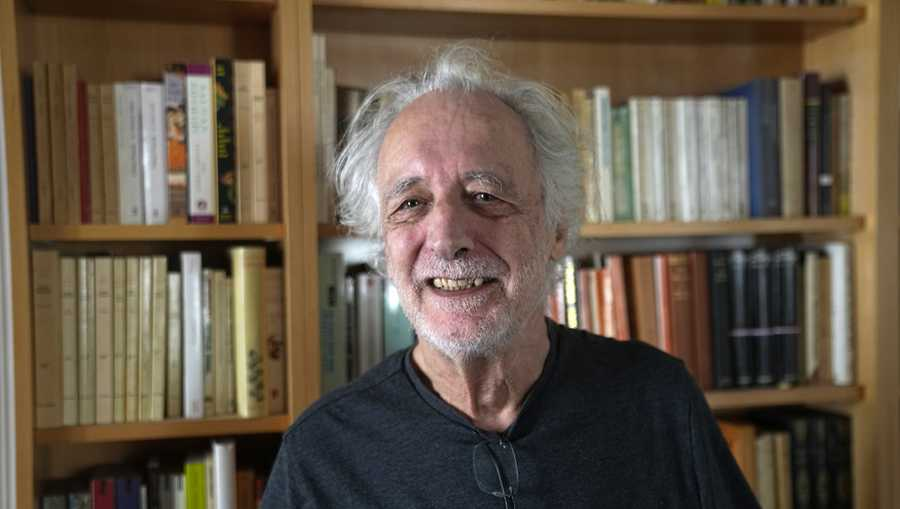
\includegraphics[width= 1\linewidth]{10}
		\caption{\small\textit{\color{timhieukhoahoc}Nhà vật lý Pháp  Pierre Agostini.}}
		\vspace*{-10pt}
	\end{figure}
	Pierre Agostini và nhóm nghiên cứu của ông tại Pháp đã thành công trong việc tạo ra và nghiên cứu một chuỗi các xung ánh sáng liên tiếp, như một đoàn tàu có nhiều toa. Họ sử dụng một kỹ thuật đặc biệt, đặt ``đoàn tàu xung" cùng với một phần bị lùi lại của xung laser ban đầu, để thấy được cách các sóng hài bậc cao đồng pha với nhau. Quá trình này cũng cho phép họ đo độ dài của các xung trong đoàn tàu, và họ nhận thấy mỗi xung chỉ dài $250$ atto giây.
	\vskip 0.1cm
	Cùng lúc đó, Ferenc Krausz và nhóm nghiên cứu của mình tại Áo đang nghiên cứu một kỹ thuật để chọn ra một xung riêng lẻ, như một toa được tách khỏi đoàn tàu và đặt sang một đường ray khác. Xung mà họ tách thành công dài $650$ atto giây và nhóm dùng nó để theo dõi và nghiên cứu một quá trình trong đó electron bị kéo ra khỏi nguyên tử.
	\vskip 0.1cm
	Những thí nghiệm này cho thấy các xung atto giây có thể được quan sát và đo, và chúng cũng có thể được sử dụng trong những thí nghiệm mới.
	\vskip 0.1cm
	Giờ thì thế giới atto giây đã mở ra, những xung ánh sáng ngắn này có thể được dùng để nghiên cứu chuyển động của electron. Hiện nay, người ta đã có thể tạo ra các xung chỉ dài vài chục atto giây, và những kỹ thuật này vẫn liên tục phát triển.
	\vskip 0.1cm
	Tiếp cận với chuyển động của electron
	\vskip 0.1cm
	Các xung atto giây cho phép đo khoảng thời gian để kéo một electron khỏi nguyên tử, và xem xét sự phụ thuộc của khoảng thời gian này vào độ chặt chẽ của liên kết giữa electron với hạt nhân nguyên tử của nó. Ngày nay, có thể xây dựng lại cách mà phân bố electron dao động từ bên này sang bên kia hoặc từ nơi này đến nơi khác trong phân tử và vật chất; trước đây vị trí của chúng chỉ có thể được đo bằng một giá trị trung bình.
	\vskip 0.1cm
	Xung atto giây có thể được dùng để kiểm tra các quá trình nội tại của vật chất, và để nhận dạng các sự kiện khác nhau. Những xung này đã được dùng để tìm hiểu vật lý chi tiết của nguyên tử và phân tử, và chúng có những ứng dụng tiềm năng trong nhiều lĩnh vực, từ điện tử đến y học.
	\vskip 0.1cm
	Chẳng hạn, xung atto giây có thể được dùng để đẩy các phân tử, khiến chúng phát ra những tín hiệu đo được. Tín hiệu phát ra từ các phân tử có cấu trúc đặc biệt, một dạng ``vân tay" giúp nhận dạng phân tử, điều này có những ứng dụng tiềm năng, bao gồm chẩn đoán y tế.
\end{multicols}
	\newpage

	\thispagestyle{empty}
	\begingroup 
	\AddToShipoutPicture*{\put(0,0){\includegraphics[width=19.5cm]{MV.pdf}}}
	\centering
	\vspace*{0cm}
	\endgroup
	\newpage	
	\pagestyle{empty}

	\setcounter{figure}{0}
	\thispagestyle{quantoannone}
\pagestyle{quantoan}
\everymath{\color{quantoan}}
\graphicspath{{../quantoan/pic/}}
%\blfootnote{\color{quantoan}\color{quantoan}$^*$Bài nói tại Viện hàn lâm Leopoldina của Berlin.}
\blfootnote{\color{quantoan}\color{quantoan}$^1$Đại học Sư phạm Hà Nội.}
\begingroup
\AddToShipoutPicture*{\put(0,616){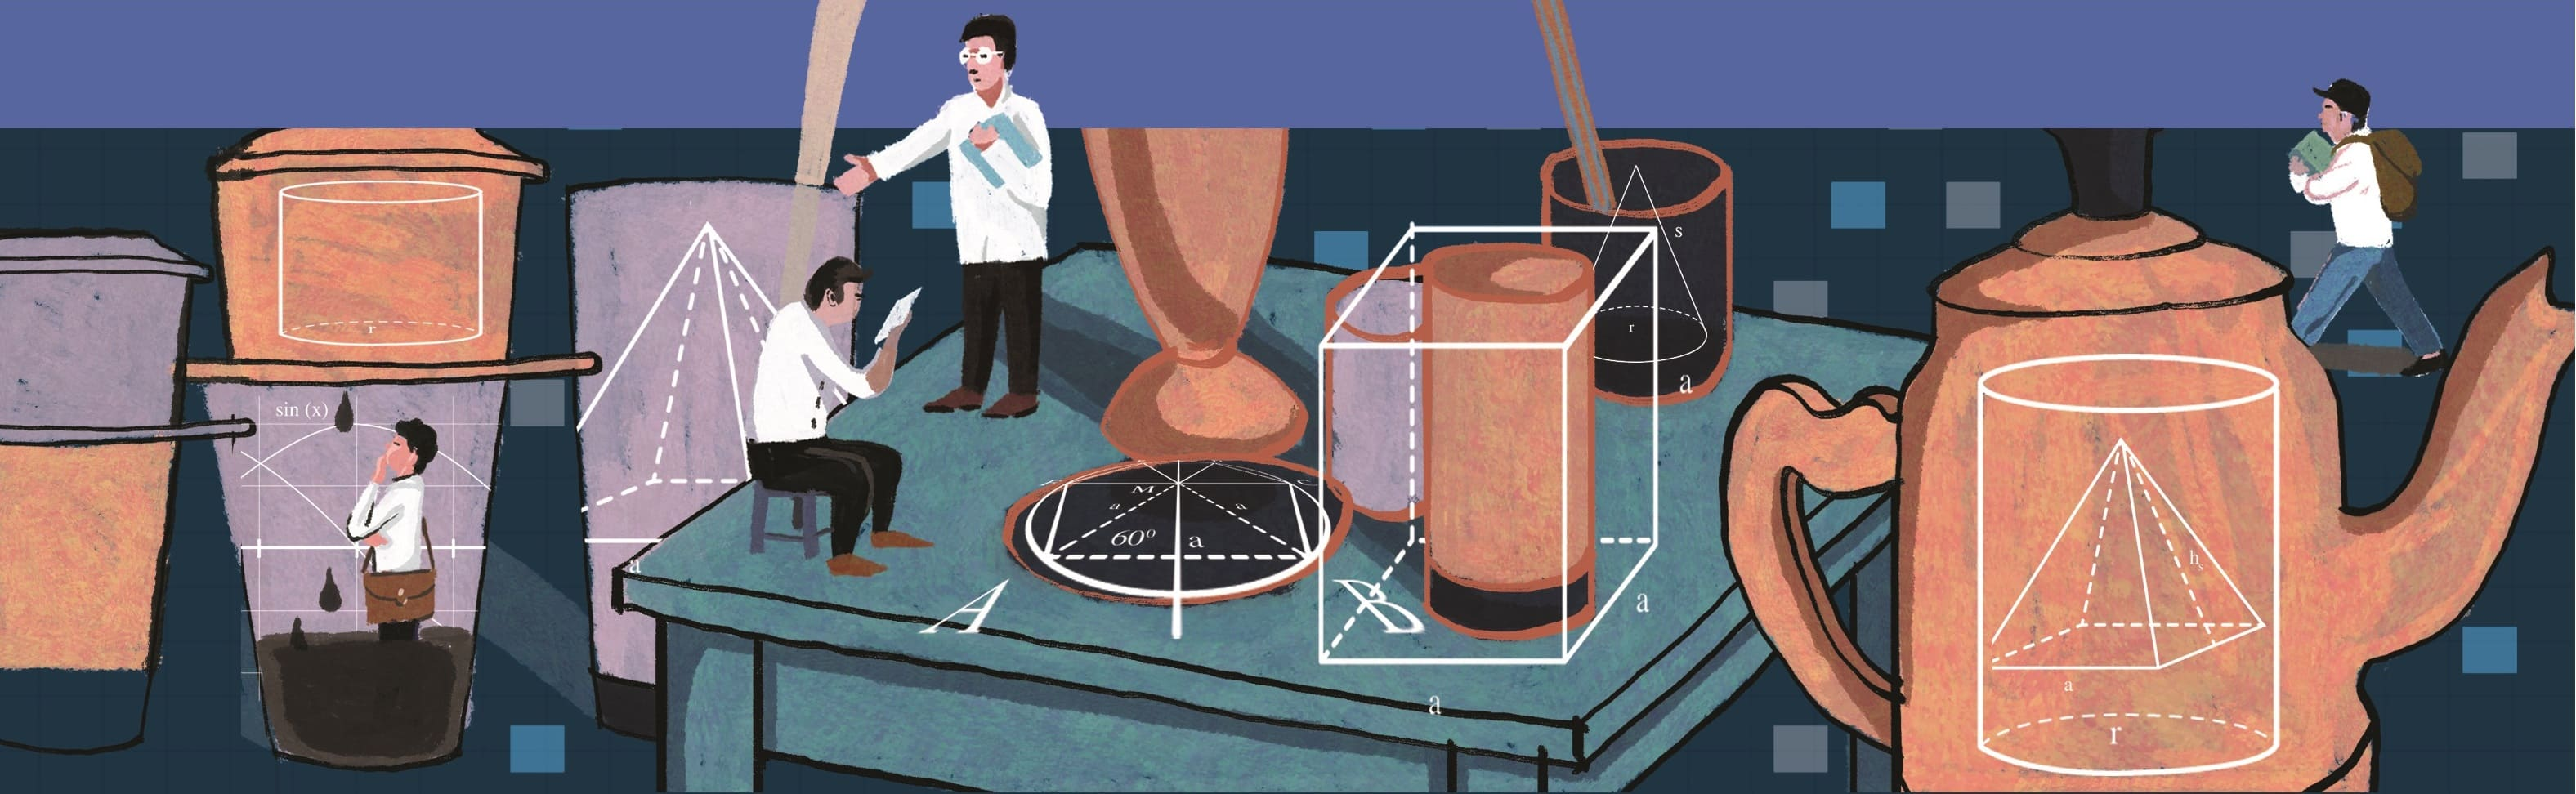
\includegraphics[width=19.3cm]{../bannerquantoan}}}
\AddToShipoutPicture*{\put(126,520){
\includegraphics[scale=1]{../tieude3.pdf}}}
\centering
\endgroup

\vspace*{182pt}

%\newpage
%\blfootnote{\color{quantoan}\color{quantoan}$^1$Đại học Sư phạm Hà Nội.}
%\begingroup
%\AddToShipoutPicture*{\put(120,675){
\includegraphics[scale=1]{../tieude3.pdf}}}
%\centering
%\endgroup
%
%
%\vspace*{35pt}

\begin{multicols}{2}
	Có một truyền thuyết  kể rằng thành phố Portland, bang Oregon đã suýt được gọi là Boston. Cuối cùng thì vấn đề đã được quyết định nhờ một cuộc tung đồng xu được tổ chức ra vào năm $1845$ giữa Francis Pettygrove, người đến từ một thành phố Portland khác, ở bang Maine, và Asa Lovejoy, đến từ Boston (người ở bang Massachusetts). Nhưng mọi chuyện có thể đã khác đi, theo Frantisek Bartos, một sinh viên tốt nghiệp tại Đại học Amsterdam, nếu con người chúng ta  không phải là những người tung xu một cách lưỡng lự thiếu dứt khoát như vậy.
	\begin{figure}[H]
		\vspace*{-5pt}
		\centering
		\captionsetup{labelformat= empty, justification=centering}
		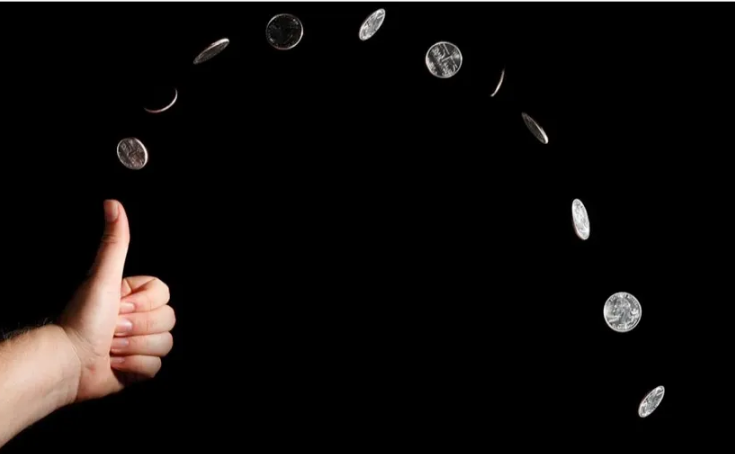
\includegraphics[width= 1\linewidth]{1111}
%		\caption{\small\textit{\color{}}}
		\vspace*{-15pt}
	\end{figure}
	Bartos đã quan tâm đến một dự đoán hấp dẫn của Persi Diaconis, Susan Holmes và Richard Montgomery, một nhóm các nhà toán học người Mỹ. Trong một bài báo đăng vào năm $2007$, bộ ba này đã phân tích tính chất vật lý của việc tung đồng xu và nhận thấy có một điều gì đó khá hấp dẫn. Bên cạnh việc khiến đồng xu quay lộn nhào, hầu hết mọi người đều có xu hướng tạo ra một sự xoay nhẹ cho đồng xu khi họ tung nó. Điều đó làm cho trục xuay mà đồng xu lật quanh đó sẽ bị trôi đẩy khi nó ở trên không trung, một hiện tượng gọi là tuế sai.
	\vskip 0.1cm
	Kết quả cuối cùng, khi các con số được xử lý, là: một đồng xu do con người ném sẽ thể hiện một xu hướng thiên vị khá tinh tế nhưng bền vững. Tiến sĩ Diaconis và các đồng nghiệp của ông tính toán có khoảng $51\%$ khả năng một đồng xu sẽ rơi theo hướng như trước khi được ném. Nói cách khác, nếu nó ngửa trong tay người ném, có nhiều khả năng hơn một chút là nó cũng sẽ chạm đất ngửa. Hoặc ít nhất, đó cũng là dự đoán.
	\vskip 0.1cm
	Bartos cùng với sự nhiệt tình đáng ngưỡng mộ của mình bắt tay vào kiểm tra thực nghiệm. Anh đã tập hợp được $48$ tình nguyện viên và thuyết phục họ thực hiện (và có quay phim) $350{.}707$ lần tung đồng xu, sử dụng hàng chục đồng xu khác nhau, từ đồng hai rupee của Ấn Độ đến đồng xu hai franc Thụy Sĩ. Dĩ nhiên, dữ liệu của anh  đã xác nhận những gì vật lý đã dự đoán. Các đồng xu đã chạm đất cùng với mặt khi tung lên tới tận $50,8\%$ số lần được ném.
	\vskip 0.1cm
	Số liệu thống kê chỉ ra rằng bản thân các đồng xu không có sự thiên vị cụ thể nào. Yếu tố quyết định thực sự đó là con người chúng ta rõ ràng không có khả năng ném thẳng.  Bartos không phải là người đầu tiên thu thập số liệu thống kê về việc tung đồng xu. Nhưng anh ta là người đầu tiên làm được điều đó ở quy mô đủ lớn để phát hiện ra sự thiên vị. (Một nỗ lực trước đó gồm $40{.}000$ lần tung, do hai sinh viên tại Đại học California, Berkeley thực hiện, đã thiếu sức mạnh thống kê để xác nhận được  lý thuyết.)
	\vskip 0.1cm
	Cơ hội $50,8\%$ chỉ khác một chút so với mức công bằng hoàn hảo. Nhưng  Bartos chỉ ra rằng cơ hội đó lớn hơn cả  lợi thế mà một sòng bạc có được trong hầu hết các loại kiểu chơi Blackjack. Và trong một số tình huống cơ hội đó có thể có vai trò quan trọng. Vào năm $2019$, Sue Cudilla trở thành thị trưởng của Araceli, một thị trấn ở Philippines, nhờ việc tung đồng xu sau khi cuộc bầu cử được tuyên bố là bất phân thắng bại. Quan trọng hơn nữa, việc tung đồng xu có thể xác định ai là người ném bóng hoặc đánh bóng trước trong môn cricket. Các vận động viên chuyên nghiệp luôn chi hàng nghìn đô la và hàng giờ tập luyện để tìm kiếm được những lợi thế cận biên. Có lẽ họ giờ  sẽ phải nên chú ý nhìn vào đồng xu lẻ trong túi quần của trọng tài.
\end{multicols}
	\newpage

	\thispagestyle{empty}
	\begingroup 
	\AddToShipoutPicture*{\put(0,0){\includegraphics[width=19.45cm]{QC}}}
	\centering
	\vspace*{0cm}
	\endgroup
	\newpage	 
	\pagestyle{empty}

	\setcounter{figure}{0}
	\thispagestyle{toancuabinone}
\pagestyle{toancuabi}
\everymath{\color{toancuabi}}
%\blfootnote{$^1$\color{toancuabi}Trường Liên cấp Hội nhập Quốc tế iSchool Quảng Trị.}
\graphicspath{{../toancuabi/pic/}}
\begingroup
\AddToShipoutPicture*{\put(0,616){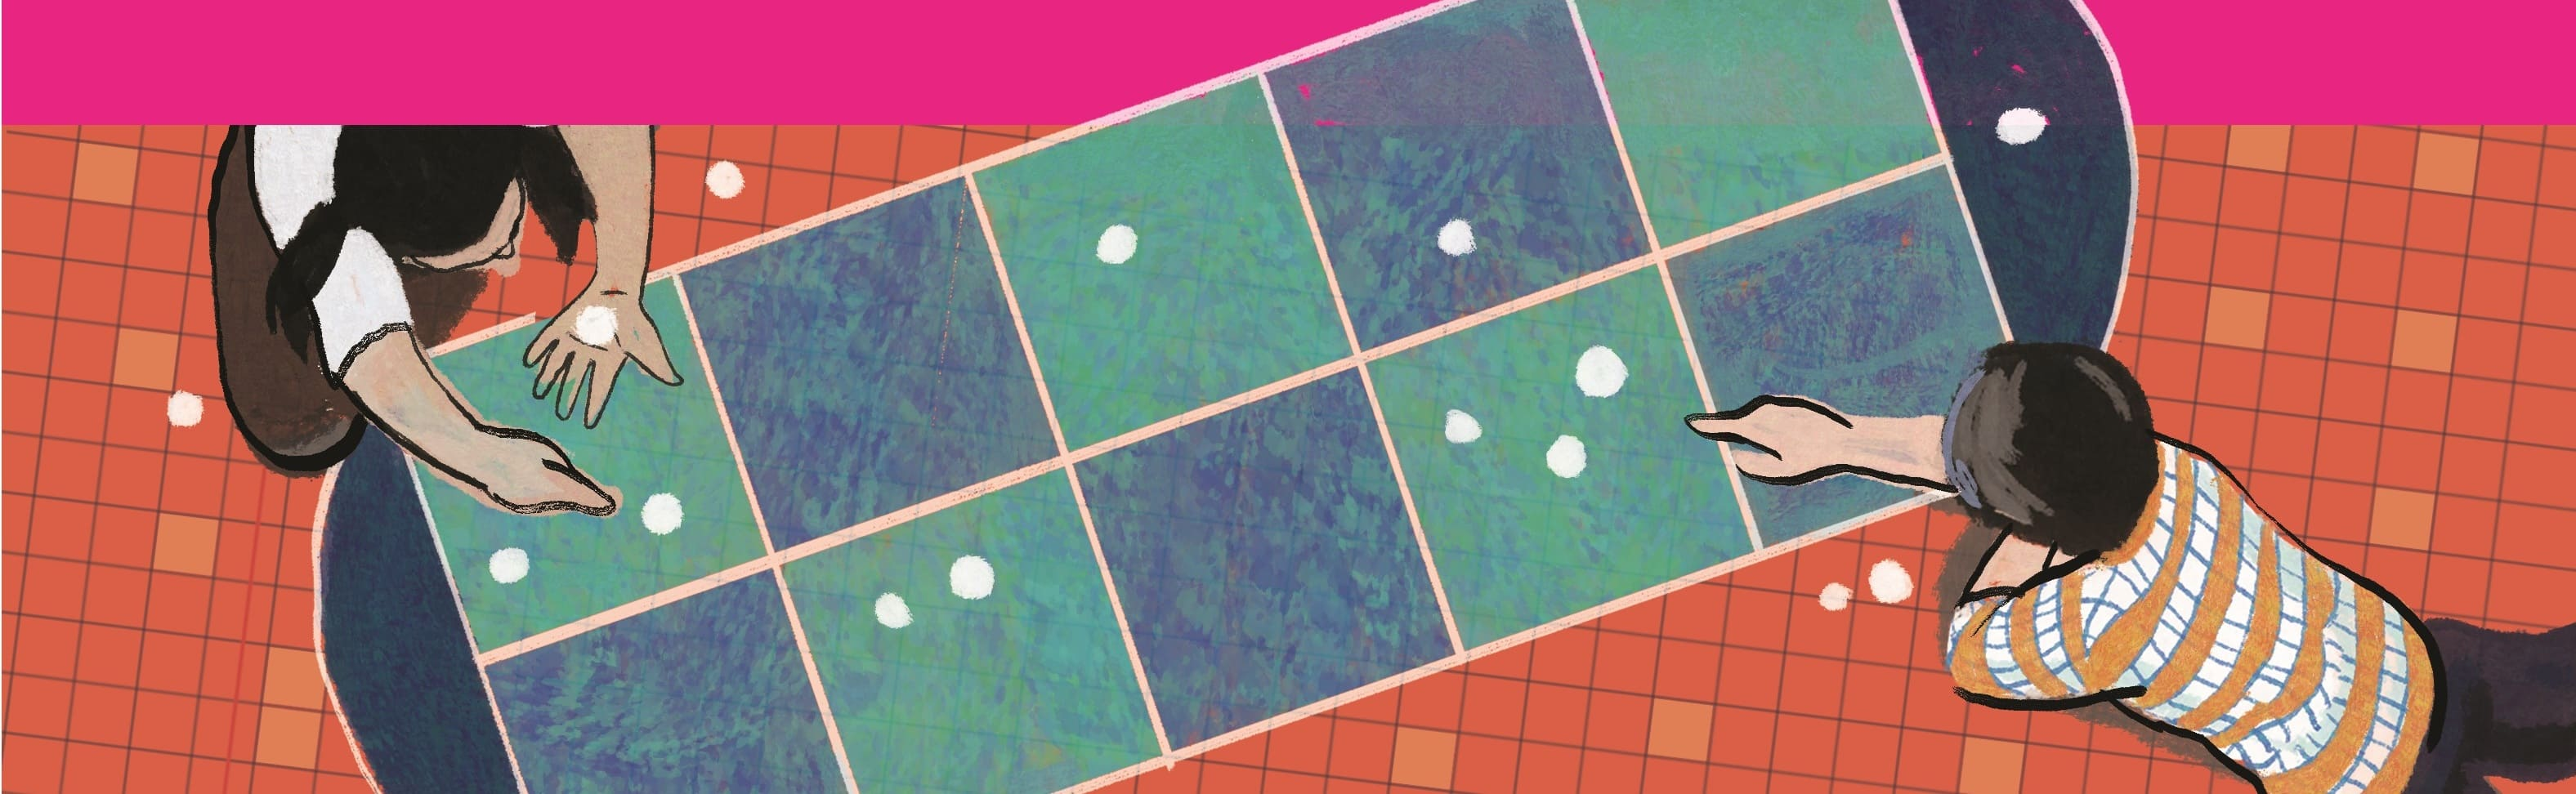
\includegraphics[width=19.3cm]{../bannertoancuabi}}}  
\AddToShipoutPicture*{\put(62,492){
\includegraphics[scale=1]{../tieude1.pdf}}}  
\centering
\endgroup
\vspace*{215pt} 

\definecolor{bulgarianrose}{rgb}{0.28, 0.02, 0.03}
\begin{multicols}{2}
	Câu lạc bộ toán học ``Unicorn Math Circle" (UMC) dành cho học sinh Tiểu học và THCS được Tạp chí Pi tổ chức từ năm $2019$, nhằm tìm kiếm và bồi dưỡng các học sinh có năng lực Toán học, tạo nguồn học sinh xuất sắc. Trong số này, tạp chí Pi giới thiệu đến bạn đọc đề thi tuyển sinh năm học $2023-2024$ dành cho các bạn học sinh lớp $4$.
	\vskip 0.1cm
	\textbf{\color{toancuabi}Bài $\pmb{1.}$} Dựa vào quy luật, hỏi hình nào trong số các hình $A$, $B$, $C$, $D$ là hình tiếp theo trong dãy sau:
	\begin{figure}[H]
		\vspace*{-5pt}
		\centering
		\captionsetup{labelformat= empty, justification=centering}
		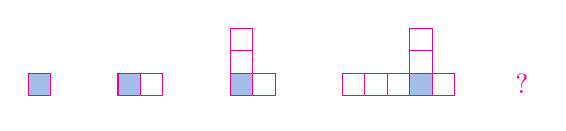
\begin{tikzpicture}[toancuabi,scale=0.285]
			\fill[cackithi!50] (-2,0) rectangle (-1,1);
			\fill[cackithi!50] (2,0) rectangle (3,1);
			\fill[cackithi!50] (7,0) rectangle (8,1);
			\fill[cackithi!50] (15,0) rectangle (16,1);
			\draw (-2,0) grid (-1,1);
			\draw (2,0) grid (4,1);
			\draw (7,0) grid (9,1);
			\draw (7,1) grid (8,3);
			\draw (12,0) grid (17,1);
			\draw (15,1) grid (16,3);
			\draw (20,0.5) node {$?$};
		\end{tikzpicture}

		\vspace*{10pt}
		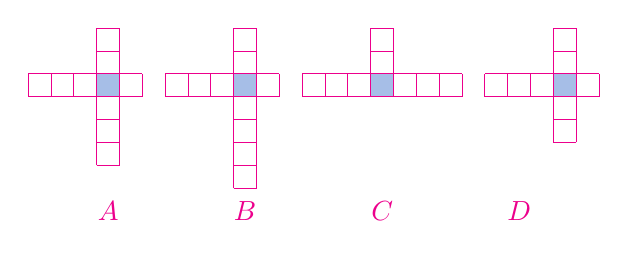
\begin{tikzpicture}[toancuabi,scale=0.29]
			\fill[cackithi!50] (3,0) rectangle (4,1);
			\fill[cackithi!50] (9,0) rectangle (10,1);
			\fill[cackithi!50] (15,0) rectangle (16,1);
			\fill[cackithi!50] (23,0) rectangle (24,1);
			\draw (0,0) grid (5,1);
			\draw (3,-3) grid (4,3);
			\draw (6,0) grid (11,1);
			\draw (9,-4) grid (10,3);
			\draw (12,0) grid (19,1);
			\draw (15, 1) grid (16,3);
			\draw (20,0) grid (25,1);
			\draw (23,-2) grid (24,3);
			
			\draw (3.5,-5) node{$A$};
			\draw (9.5,-5) node{$B$};
			\draw (15.5,-5) node{$C$};
			\draw (21.5,-5) node{$D$};
		\end{tikzpicture}
		\vspace*{-15pt}
	\end{figure}
	\textbf{\color{toancuabi}Bài $\pmb{2.}$} Một cặp số có hai chữ số như $18$ và $81$ được gọi là cặp \textit{bạn thân} vì chúng có chữ số hàng chục và chữ số hàng đơn vị đổi chỗ cho nhau. Hỏi có bao nhiêu cặp bạn thân mà tổng của chúng bằng $99$?
	\vskip 0.1cm
	\textbf{\color{toancuabi}Bài $\pmb{3.}$} Bạn Ngọc được tặng một thanh sô--cô--la hình trái tim. Mỗi ô vuông có trọng lượng $8$g. Hỏi thanh sô--cô--la có khối lượng bằng bao nhiêu?
	\begin{figure}[H]
		\vspace*{-5pt}
		\centering
		\captionsetup{labelformat= empty, justification=centering}
		\begin{tikzpicture}[scale=0.6]
			\clip (0,0) - ++(0,2) - ++(2,4) - ++(4,2) - ++(6,4) - ++(8,2) - ++(8,0) - ++(4,-4) -- cycle;;
			\draw[fill=bulgarianrose!90] (0,0) - ++(0,2) - ++(2,4) - ++(4,2) - ++(6,4) - ++(8,2) - ++(8,0) - ++(4,-4) -- cycle;
			\draw (0,0) - ++(0,2) - ++(2,4) - ++(4,2) - ++(6,4) - ++(8,2) - ++(8,0) - ++(4,-4) -- cycle;
			\draw (0,-4) grid (8,4);
		\end{tikzpicture}
		\vspace*{-5pt}
	\end{figure}
	\textbf{\color{toancuabi}Bài $\pmb{4.}$} Trong hình vẽ sau, mỗi miền được tô $1$ màu, không có $2$ miền nào cùng màu. Có bao nhiêu miền nằm trong ít nhất $3$ hình tròn?	 
	\begin{figure}[H]
		\vspace*{-5pt}
		\centering
		\captionsetup{labelformat= empty, justification=centering}
		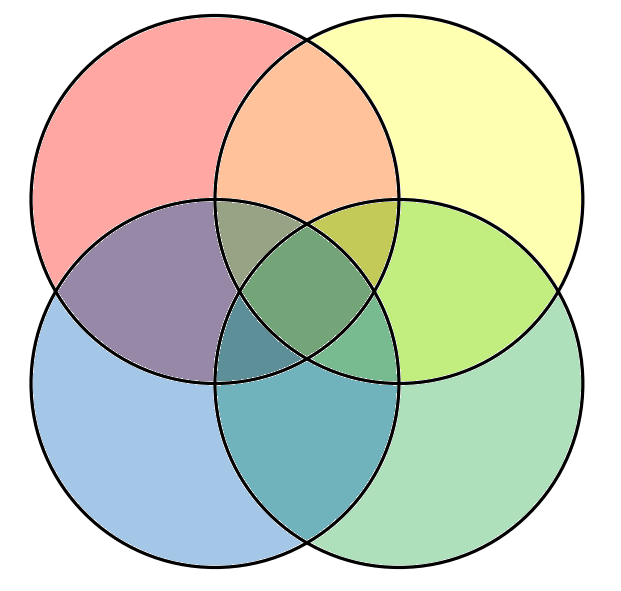
\includegraphics[width= 0.65\linewidth]{2}
%		\caption{\small\textit{\color{}}}
		\vspace*{-5pt}
	\end{figure}
	\textbf{\color{toancuabi}Bài $\pmb{5.}$} Số $1995$ được xếp bằng các que diêm như hình dưới đây. An dịch chuyển đúng $1$ que diêm để nhận được số lớn nhất có thể. Hỏi số đó bằng bao nhiêu?
	\begin{figure}[H]
		\vspace*{-5pt}
		\centering
		\captionsetup{labelformat= empty, justification=centering}
		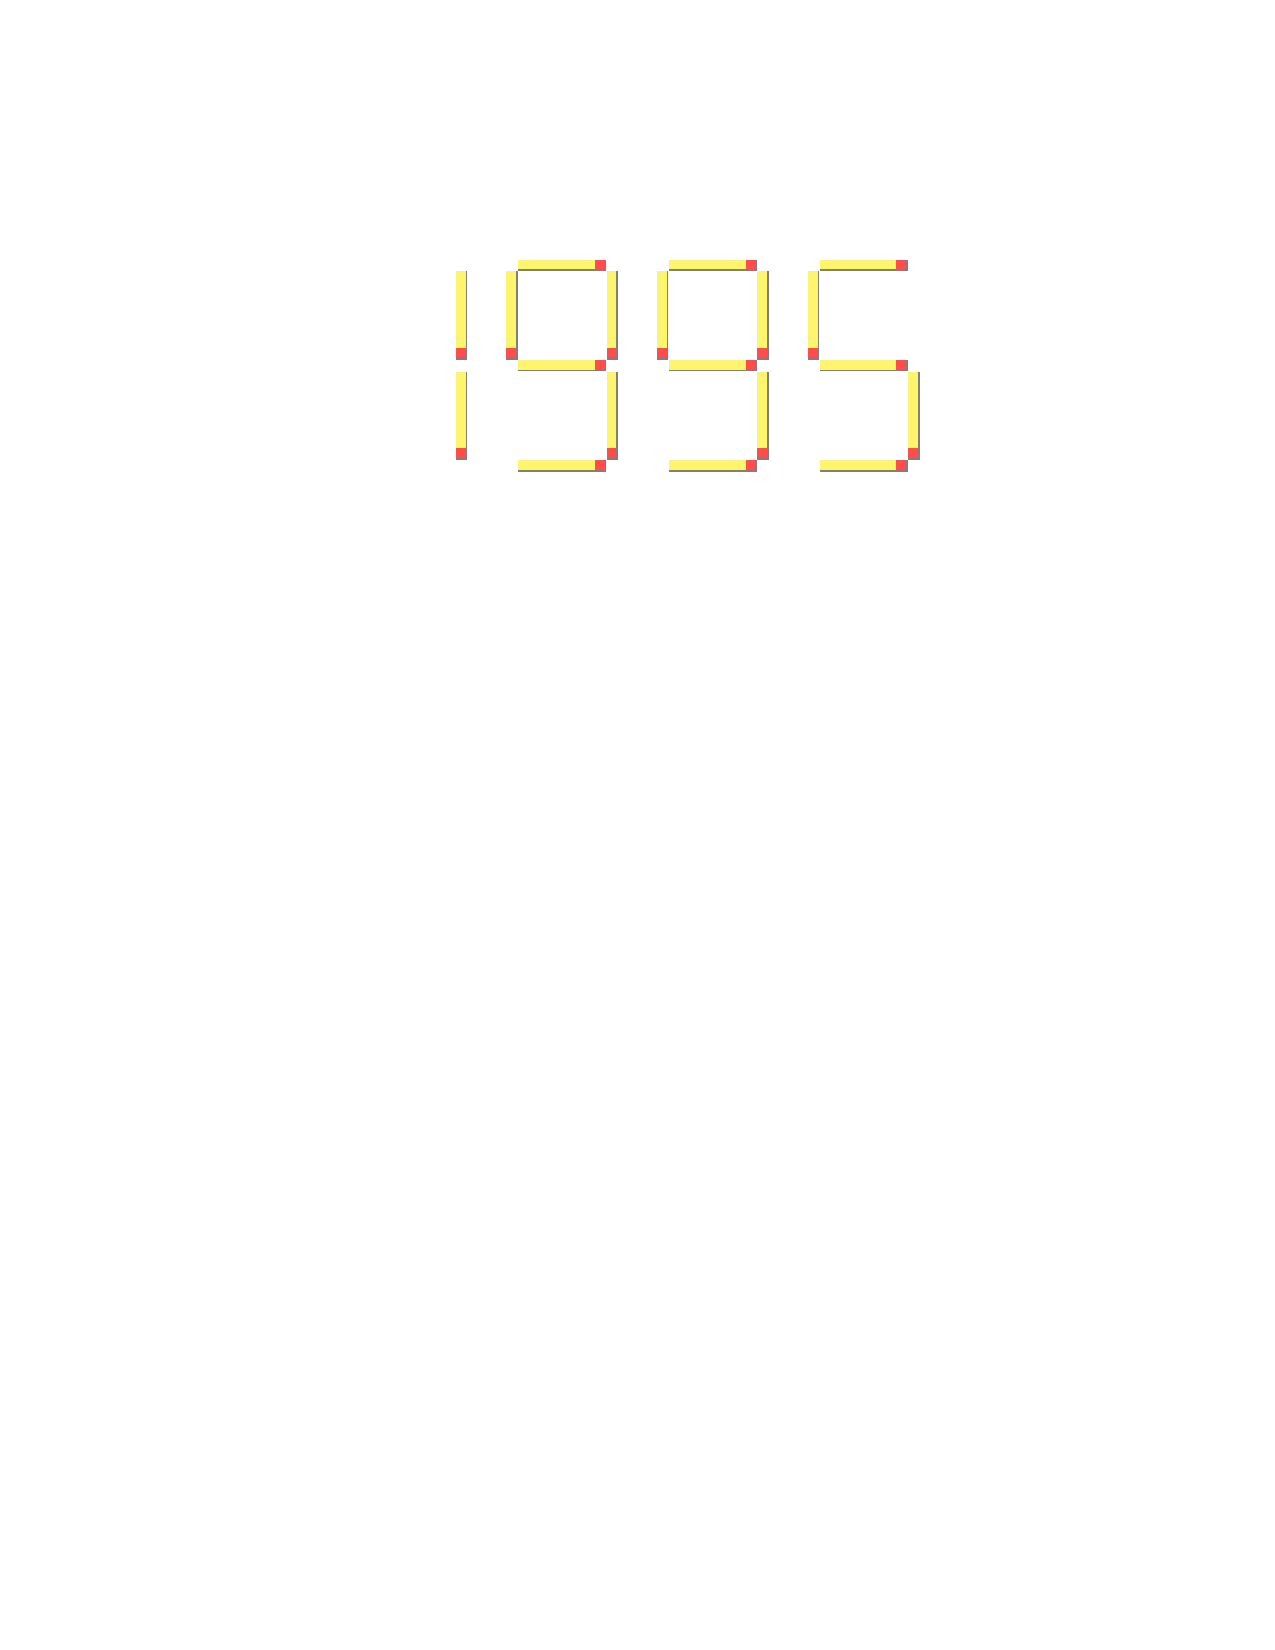
\includegraphics[width= 1\linewidth]{3}
%		\caption{\small\textit{\color{}}}
		\vspace*{-15pt}
	\end{figure}
	\textbf{\color{toancuabi}Bài $\pmb{6.}$} Như hình vẽ, có $9$ ô vuông nhỏ, vẽ một đường thẳng, hỏi đường thẳng này đi qua nhiều nhất bao nhiêu ô vuông nhỏ?
	\begin{figure}[H]
		\vspace*{-5pt}
		\centering
		\captionsetup{labelformat= empty, justification=centering}
		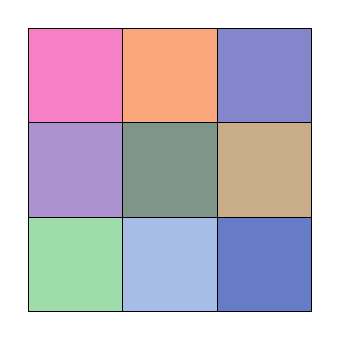
\begin{tikzpicture}[scale=1.2]
			\draw[fill=diendantoanhoc!50] (0,0) rectangle (1,1);
			\draw[fill=gocco!50] (0,1) rectangle (1,2);
			\draw[fill=toancuabi!50] (0,2) rectangle (1,3);
			\draw[fill=cackithi!50] (1,0) rectangle (2,1);
			\draw[fill=thachthuctoanhoc!50] (1,1) rectangle (2,2);
			\draw[fill=duongvaotoanhoc!50] (1,2) rectangle (2,3);
			\draw[fill=quantoan!80] (2,0) rectangle (3,1);
			\draw[fill=lichsutoanhoc!50] (2,1) rectangle (3,2);
			\draw[fill=timhieukhoahoc!60] (2,2) rectangle (3,3);
			\draw (0,0) grid (3,3);
		\end{tikzpicture}
		\vspace*{-5pt}
	\end{figure}
	\textbf{\color{toancuabi}Bài $\pmb{7.}$} Trong hình vẽ bên dưới, hình ngôi sao lớn được chia thành các hình tam giác có chu vi bằng $7$, các hình tứ giác có chu vi bằng $18$ và một hình ngôi sao nhỏ có chu vi bằng $3$. Tìm chu vi của hình ngôi sao lớn ban đầu.
	\begin{figure}[H]
		\vspace*{-5pt}
		\centering
		\captionsetup{labelformat= empty, justification=centering}
		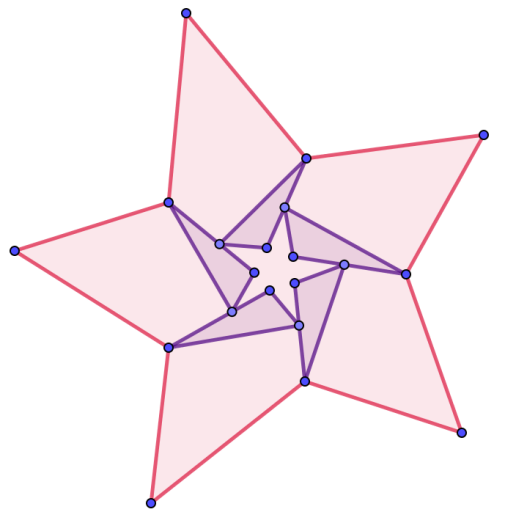
\includegraphics[width= 0.7\linewidth]{5}
%		\caption{\small\textit{\color{}}}
%		\vspace*{-10pt}
	\end{figure}
	\textbf{\color{toancuabi}Bài $\pmb{8.}$} Trong siêu thị có sự kiện ra mắt một loại kem mới, để quảng cáo loại kem này, họ cho phép cứ $2$ cái vỏ kem đổi được $1$ cây kem, bạn Bảo Châu mua $10$ que kem, vậy bạn ấy thực sự có thể ăn được nhiều nhất bao nhiêu que kem?
	\vskip 0.1cm
	\textbf{\color{toancuabi}Bài $\pmb{9.}$} Một hình vuông to được chia thành các hình vuông nhỏ hơn với nhiều kích cỡ, trong đó một số được tô màu hồng như hình vẽ. Biết diện tích phần màu trắng của hình vuông là $180$. Tìm diện tích phần màu hồng của hình vuông.
	\begin{figure}[H]
	\vspace*{-5pt}
	\centering
	\captionsetup{labelformat= empty, justification=centering}
	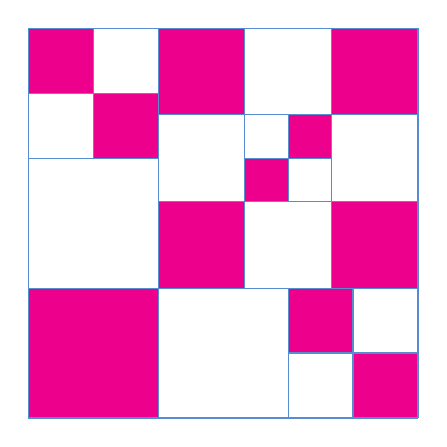
\begin{tikzpicture}[scale=0.55, cackithi]
		\fill[fill=toancuabi] (-2.,7.) -- (-2.,5.5) -- (-0.5,5.5) -- (-0.5,7.) -- cycle;
		\fill[fill=toancuabi] (-0.5,5.5) -- (-0.5,4.) -- (1.,4.) -- (1.,5.5) -- cycle;
		\fill[fill=toancuabi] (1.,7.) -- (1.,5.) -- (3.,5.) -- (3.,7.) -- cycle;
		\fill[fill=toancuabi] (5.,7.) -- (5.,5.) -- (7.,5.) -- (7.,7.) -- cycle;
		\fill[fill=toancuabi] (4.,5.) -- (4.,4.) -- (5.,4.) -- (5.,5.) -- cycle;
		\fill[fill=toancuabi] (3.,4.) -- (3.,3.) -- (4.,3.) -- (4.,4.) -- cycle;
		\fill[fill=toancuabi] (5.,3.) -- (5.,1.) -- (7.,1.) -- (7.,3.) -- cycle;
		\fill[fill=toancuabi] (1.,3.) -- (1.,1.) -- (3.,1.) -- (3.,3.) -- cycle;
		\fill[fill=toancuabi] (4.,1.) -- (4.,-0.5) -- (5.5,-0.5) -- (5.5,1.) -- cycle;
		\fill[fill=toancuabi] (5.5,-0.5) -- (5.5,-2.) -- (7.,-2.) -- (7.,-0.5) -- cycle;
		\fill[fill=toancuabi] (-2.,1.) -- (-2.,-2.) -- (1.,-2.) -- (1.,1.) -- cycle;
		\draw  (3.,5.)-- (5.,5.);
		\draw  (5.,5.)-- (5.,3.);
		\draw  (5.,3.)-- (3.,3.);
		\draw  (3.,3.)-- (3.,5.);
		\draw  (4.,5.)-- (4.,3.);
		\draw  (3.,4.)-- (5.,4.);
		\draw  (7.,5.)-- (7.,3.);
		\draw  (7.,3.)-- (5.,3.);
		\draw  (3.,5.)-- (1.,5.);
		\draw  (1.,5.)-- (1.,3.);
		\draw  (1.,3.)-- (3.,3.);
		\draw  (1.,3.)-- (1.,1.);
		\draw  (1.,1.)-- (7.,1.);
		\draw  (7.,1.)-- (7.,3.);
		\draw  (5.,3.)-- (5.,1.);
		\draw  (3.,3.)-- (3.,1.);
		\draw  (1.,5.)-- (1.,7.);
		\draw  (1.,7.)-- (7.,7.);
		\draw  (7.,7.)-- (7.,5.);
		\draw  (5.,5.)-- (5.,7.);
		\draw  (3.,5.)-- (3.,7.);
		\draw  (1.,7.)-- (-2.,7.);
		\draw  (-2.,7.)-- (-2.,1.);
		\draw  (1.,4.)-- (-2.,4.);
		\draw  (-2.,-2.)-- (7.,-2.);
		\draw  (7.,-2.)-- (7.,1.);
		\draw  (4.,1.)-- (4.,-2.);
		\draw  (-2.,7.)-- (-2.,5.5);
		\draw  (-2.,5.5)-- (-0.5,5.5);
		\draw  (-0.5,5.5)-- (-0.5,7.);
		\draw  (-0.5,7.)-- (-2.,7.);
		\draw  (-0.5,5.5)-- (-0.5,4.);
		\draw  (-0.5,4.)-- (1.,4.);
		\draw  (1.,4.)-- (1.,5.5);
		\draw  (1.,5.5)-- (-0.5,5.5);
		\draw  (1.,7.)-- (1.,5.);
		\draw  (1.,5.)-- (3.,5.);
		\draw  (3.,5.)-- (3.,7.);
		\draw  (3.,7.)-- (1.,7.);
		\draw  (5.,7.)-- (5.,5.);
		\draw  (5.,5.)-- (7.,5.);
		\draw  (7.,5.)-- (7.,7.);
		\draw  (7.,7.)-- (5.,7.);
		\draw  (4.,5.)-- (4.,4.);
		\draw  (4.,4.)-- (5.,4.);
		\draw  (5.,4.)-- (5.,5.);
		\draw  (5.,5.)-- (4.,5.);
		\draw  (3.,4.)-- (3.,3.);
		\draw  (3.,3.)-- (4.,3.);
		\draw  (4.,3.)-- (4.,4.);
		\draw  (4.,4.)-- (3.,4.);
		\draw  (5.,3.)-- (5.,1.);
		\draw  (5.,1.)-- (7.,1.);
		\draw  (7.,1.)-- (7.,3.);
		\draw  (7.,3.)-- (5.,3.);
		\draw  (1.,3.)-- (1.,1.);
		\draw  (1.,1.)-- (3.,1.);
		\draw  (3.,1.)-- (3.,3.);
		\draw  (3.,3.)-- (1.,3.);
		\draw  (4.,1.)-- (4.,-0.5);
		\draw  (4.,-0.5)-- (5.5,-0.5);
		\draw  (5.5,-0.5)-- (5.5,1.);
		\draw  (5.5,1.)-- (4.,1.);
		\draw  (5.5,-0.5)-- (5.5,-2.);
		\draw  (5.5,-2.)-- (7.,-2.);
		\draw  (7.,-2.)-- (7.,-0.5);
		\draw  (7.,-0.5)-- (5.5,-0.5);
		\draw  (-2.,1.)-- (-2.,-2.);
		\draw  (-2.,-2.)-- (1.,-2.);
		\draw  (1.,-2.)-- (1.,1.);
		\draw  (1.,1.)-- (-2.,1.);
	\end{tikzpicture}
	\vspace*{-5pt}
	\end{figure}
	\textbf{\color{toancuabi}Bài $\pmb{10.}$} Hai bạn Nam và Dương đi chợ sách và nhìn thấy cuốn tạp chí Pi. Nam muốn mua $1$ cuốn nhưng thiếu $12$ nghìn đồng. Dương muốn mua $1$ cuốn nhưng thiếu $23$ nghìn đồng. Nếu $2$ bạn chung tiền mua thì vừa đủ mua $1$ cuốn. Hỏi cuốn tạp chí Pi giá bao nhiêu tiền?
	\end{multicols}
	\newpage
	\begin{multicols}{2}
	\textbf{\color{toancuabi}Lời giải.}
	\vskip 0.1cm
	\textbf{\color{toancuabi}Bài $\pmb{1.}$} Ta thấy nếu lấy ô vuông được tô màu làm tâm, thì theo ngược chiều kim đồng hồ số các ô vuông kề với tâm sẽ tăng dần: $1,2,3,4$. Do đó hình $B$ là hình tiếp theo trong dãy.
	\vskip 0.1cm
	\textbf{\color{toancuabi}Bài $\pmb{2.}$} Ta có thể thấy ngay cặp số bạn thân có tổng bằng $99$ thì mỗi số trong cặp có tổng chữ số hàng chục và hàng đơn vị bằng $9$. Do $9 = 1+8 = 2+7 = 3+6 = 4+5$ nên ta có $4$ cặp số bạn thân thỏa mãn là: $18-81$, $27-72$, $36-63$, $45-54$.
	\vskip 0.1cm
	\textbf{\color{toancuabi}Bài $\pmb{3.}$} Thanh sô--cô--la hình trái tim được ghép từ $32$ miếng ô vuông và $16$ miếng nửa ô vuông. Sau khi ghép các nửa ô vuông lại với nhau, thì ta thấy thanh sô--cô--la gồm $40$ ô. Do đó khối lượng của thanh sô--cô--la là: $4\times 80=320 \text{ (g)}$.
	\vskip 0.1cm
	\textbf{\color{toancuabi}Bài $\pmb{4.}$} Đánh số các miền như trong hình dưới đây. Ta thấy các miền $4$, $5$, $7$, $9$ và $10$ nằm trong ít nhất $3$ hình tròn. Do đó có $5$ miền thỏa mãn đề bài.
	\begin{figure}[H]
		\vspace*{-5pt}
		\centering
		\captionsetup{labelformat= empty, justification=centering}
		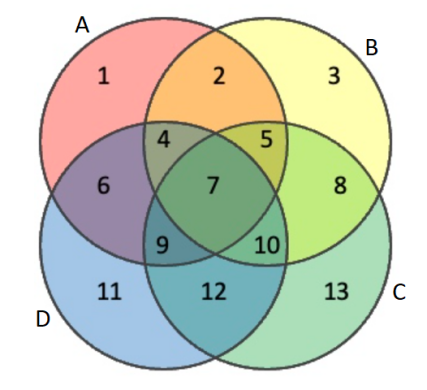
\includegraphics[width= 0.7\linewidth]{7}
%		\caption{\small\textit{\color{}}}
		\vspace*{-10pt}
	\end{figure}
	\textbf{\color{toancuabi}Bài $\pmb{5.}$} Bạn An di chuyển một que diêm từ chữ số $9$ hàng chục sang chữ số $1$ hàng nghìn và được số lớn nhất là:  
	\begin{figure}[H]
		\vspace*{-5pt}
		\centering
		\captionsetup{labelformat= empty, justification=centering}
		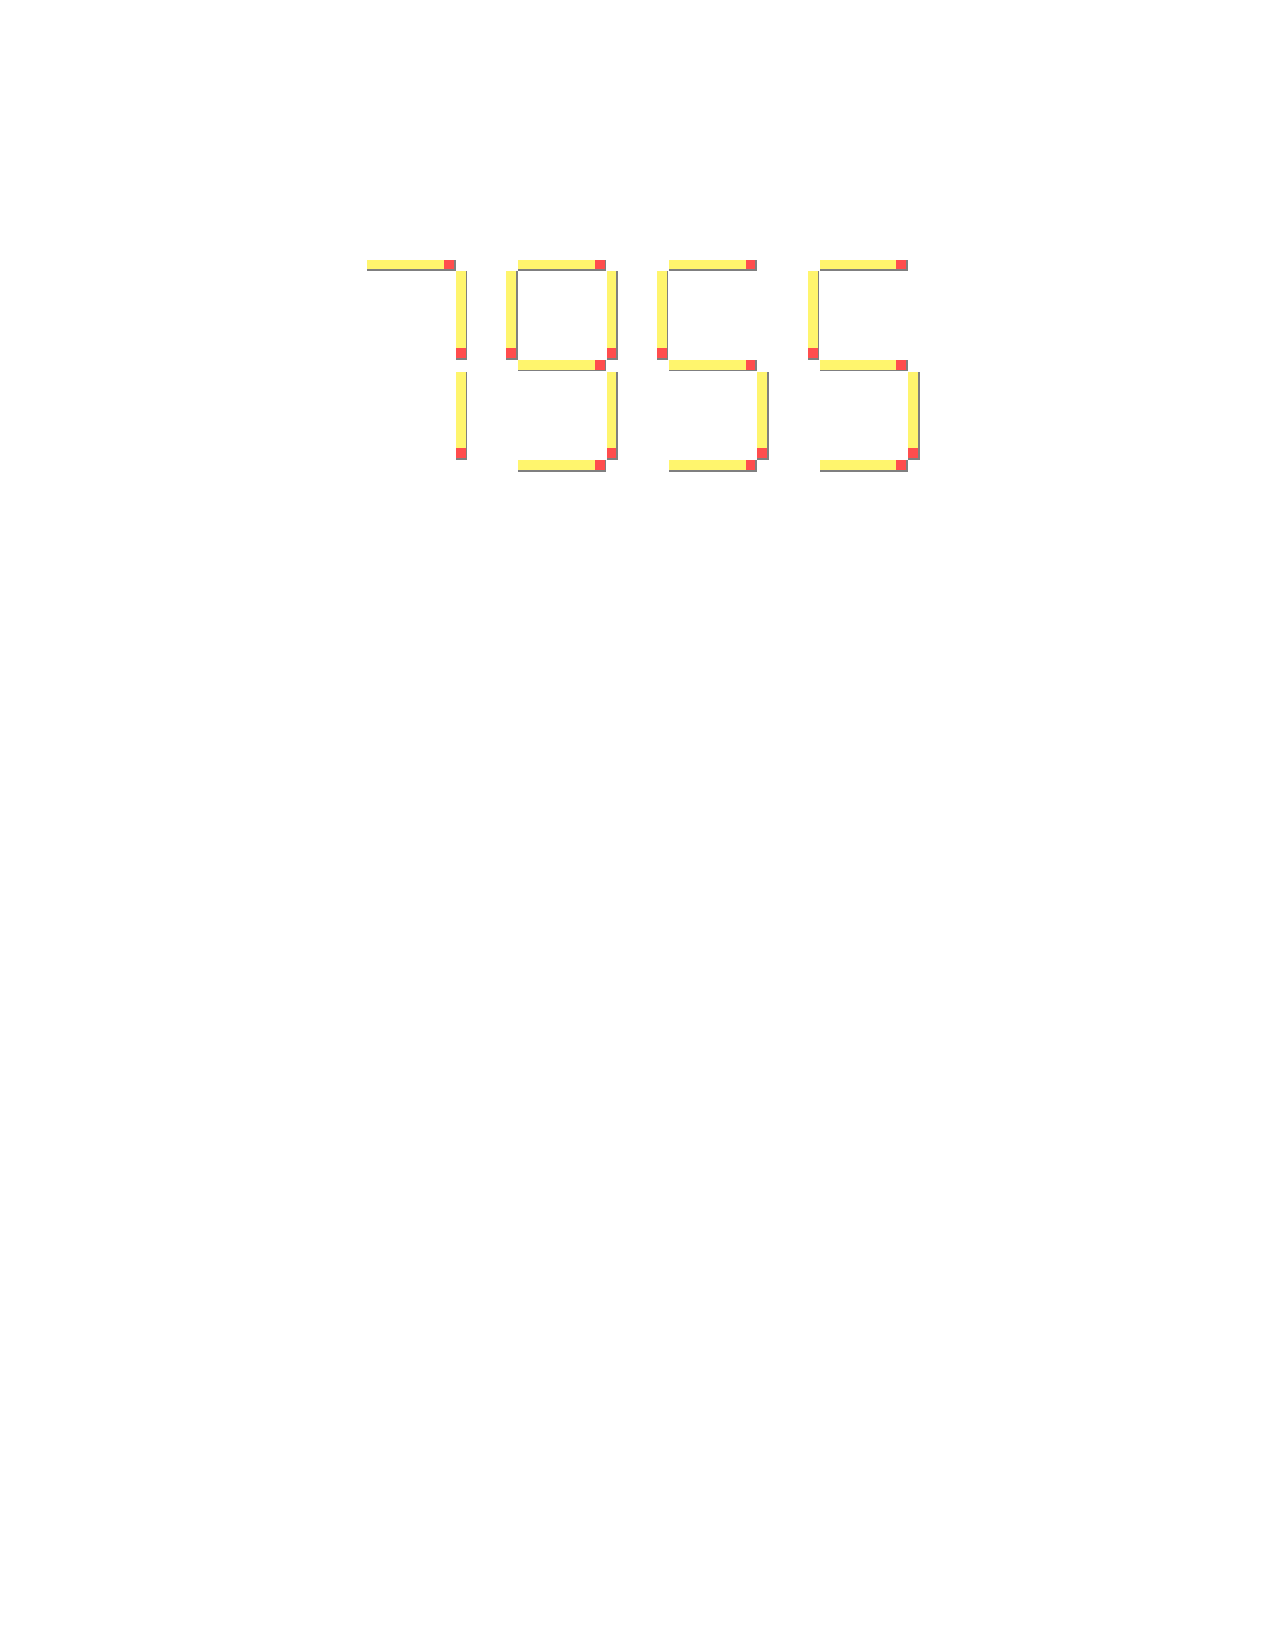
\includegraphics[width= 1\linewidth]{8}
%		\caption{\small\textit{\color{}}}
		\vspace*{-15pt}
	\end{figure}
	\textbf{\color{toancuabi}Bài $\pmb{6.}$} Ta vẽ đường thẳng như hình dưới đây, khi đó đường thẳng đi qua nhiều nhất $5$ ô vuông nhỏ.
	\begin{figure}[H]
		\vspace*{-5pt}
		\centering
		\captionsetup{labelformat= empty, justification=centering}
		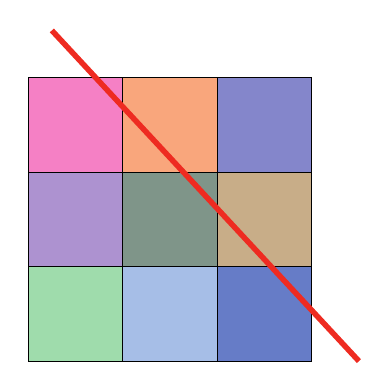
\begin{tikzpicture}[scale=1.2]
			\draw[fill=diendantoanhoc!50] (0,0) rectangle (1,1);
			\draw[fill=gocco!50] (0,1) rectangle (1,2);
			\draw[fill=toancuabi!50] (0,2) rectangle (1,3);
			\draw[fill=cackithi!50] (1,0) rectangle (2,1);
			\draw[fill=thachthuctoanhoc!50] (1,1) rectangle (2,2);
			\draw[fill=duongvaotoanhoc!50] (1,2) rectangle (2,3);
			\draw[fill=quantoan!80] (2,0) rectangle (3,1);
			\draw[fill=lichsutoanhoc!50] (2,1) rectangle (3,2);
			\draw[fill=timhieukhoahoc!60] (2,2) rectangle (3,3);
			\draw (0,0) grid (3,3);
			\draw[line width= 2pt, toanhocdoisong] (0.25,3.5) -- (3.5,0); 
		\end{tikzpicture}
%		\vspace*{-5pt}
	\end{figure}
	\textbf{\color{toancuabi}Bài $\pmb{7.}$} Tổng các cạnh của các hình tứ giác mà không phải là cạnh của ngôi sao lớn là:
	\begin{align*}
		7\times 5-3 = 32 \text{ (đơn vị).}
	\end{align*}
	Vậy chu vi của ngôi sao lớn ban đầu là:
	\begin{align*}
		18\times 5-32 = 58 \text{ (đơn vị).}
	\end{align*}
	\textbf{\color{toancuabi}Bài $\pmb{8.}$}  Đầu tiên bạn Châu đổi được $10:2=5$ (que kem). Với $5$ que kem mới này bạn đổi được $5:2=2$ que kem và dư $1$ vỏ que kem. Với $2$ vỏ que kem bạn Châu lại tiếp tục đổi được $1$ que kem. Cuối cùng $1$ vỏ que kem này và $1$ vỏ que kem còn thừa trước đó, bạn lại đổi được $1$ que kem nữa. Vậy tổng cộng bạn Châu được ăn số que kem là: 
	\begin{align*}
		10+5+2+1+1=19 \text{ (que kem).}
	\end{align*}
	\textbf{\color{toancuabi}Bài $\pmb{9.}$} Bằng cách ghép các phần được tô hồng như trong các minh họa dưới đây, ta thấy phần màu hồng gồm $4$ ô vuông nhỏ và phần màu trắng gồm $5$ ô vuông nhỏ cùng kích thước.
	\begin{figure}[H]
		\vspace*{-5pt}
		\centering
		\captionsetup{labelformat= empty, justification=centering}
		
\includegraphics[width= 1\linewidth]{10a.pdf}
		%		\caption{\small\textit{\color{}}}
		\vspace*{-15pt}
	\end{figure}
	Như vậy diện tích một ô vuông nhỏ là: 
	\begin{align*}
		180:5 = 36 \text{ (đơn vị).}
	\end{align*}
	Do đó diện tích phần được tô hồng là: 
	\begin{align*}
		36\times 4 = 144 \text{ (đơn vị).}
	\end{align*}
	\textbf{\color{toancuabi}Bài $\pmb{10.}$} Vì hai bạn chung tiền mua thì vừa đủ $1$ cuốn tạp chí Pi, nên số tiền mà Nam còn thiếu chính là số tiền mà Dương có, số tiền mà Dương thiếu chính là số tiền mà Nam có. Vậy Dương có $12$ nghìn, Nam có $23$ nghìn. Vậy cuốn tạp chí Pi giá $12+23=35$ (nghìn).
\end{multicols}
\newpage
\graphicspath{{../toancuabi/pic/}}
\begingroup
\AddToShipoutPicture*{\put(106,650){
\includegraphics[scale=1]{../tieude.pdf}}}  
\centering
\endgroup
\vspace*{55pt} 
\begin{multicols}{2}
	Thám tử Xuân Phong đôi khi phải đột nhập vào những nơi hoang vắng, kỳ bí để tìm ra được dấu tích của những kẻ gây án. Một lần nọ, sau bao ngày cải trang để bám sát, theo dõi manh mối, thám tử biết tên trùm tội phạm đang trốn tránh trong một ngôi nhà hẻo lánh ở ngoại ô. Vừa đến trước cửa của ngôi nhà gỗ cổ kính, Xuân Phong gặp một bà lão với đôi mắt tinh anh nhìn mình với vẻ bí mật ``Thám tử đó phải không, tôi nhận ngay ra ngài, dù ngài đã cải trang rất kỹ. Phải chăng thám tử đang đi tìm tên trùm? Hắn đang ngồi dưới kia, trong căn phòng cùng những người trong hiệp hội Thương Gia, nhưng vô cùng nguy hiểm nếu ngài dùng vũ lực ở đây để bắt hắn. Tôi mách ngài nhé, ở dưới đó, có $10$ người, trong đó có lão trùm và những kẻ đồng phạm của lão. Bọn họ là những kẻ luôn nói dối, nhưng cũng có thể có cả những người lương thiện, luôn nói thật, ở ngay bên cạnh. Ngài hãy dùng trí thông minh của mình, chỉ được hỏi rất hạn chế câu hỏi để phán đoán ra những kẻ phạm tội là ai. Ngài hỏi nhiều câu hơn sẽ nguy hiểm cho cả những Thương gia lương thiện có thể có mặt ở đó. Và ngài hãy hứa với bà lão này sẽ đảm bảo an toàn cho tôi và gia đình, vì tôi đã liều mình thông báo tin mật này với Thám tử".
	\vskip 0.1cm
	Theo lời bà lão mách bảo, Xuân Phong lần theo một chiếc cầu thang cũ nát và đi xuống một căn phòng khuất dưới tầng hầm. Vừa mở cửa ra, thám tử đã thấy có $10$ người ăn mặc chỉnh tề như nhau, ngồi nghiêm trang quanh một chiếc bàn mười cạnh, mỗi người ngồi tại đỉnh của hình mười cạnh. Ánh sáng lờ mờ trong phòng đủ chiếu rõ dòng chữ ``Cuộc họp thường niên Hiệp hội Thương gia -- Khu vực Duyên Hải". Thật khó để xác định ai là kẻ nói dối trong số họ, vì vẻ ngoài họ đều giống như những Thương Gia thường gặp: quyền lực, sắc sảo và oai vệ.
	\begin{figure}[H]
		\centering
		\vspace*{-5pt}
		\captionsetup{labelformat= empty, justification=centering}
		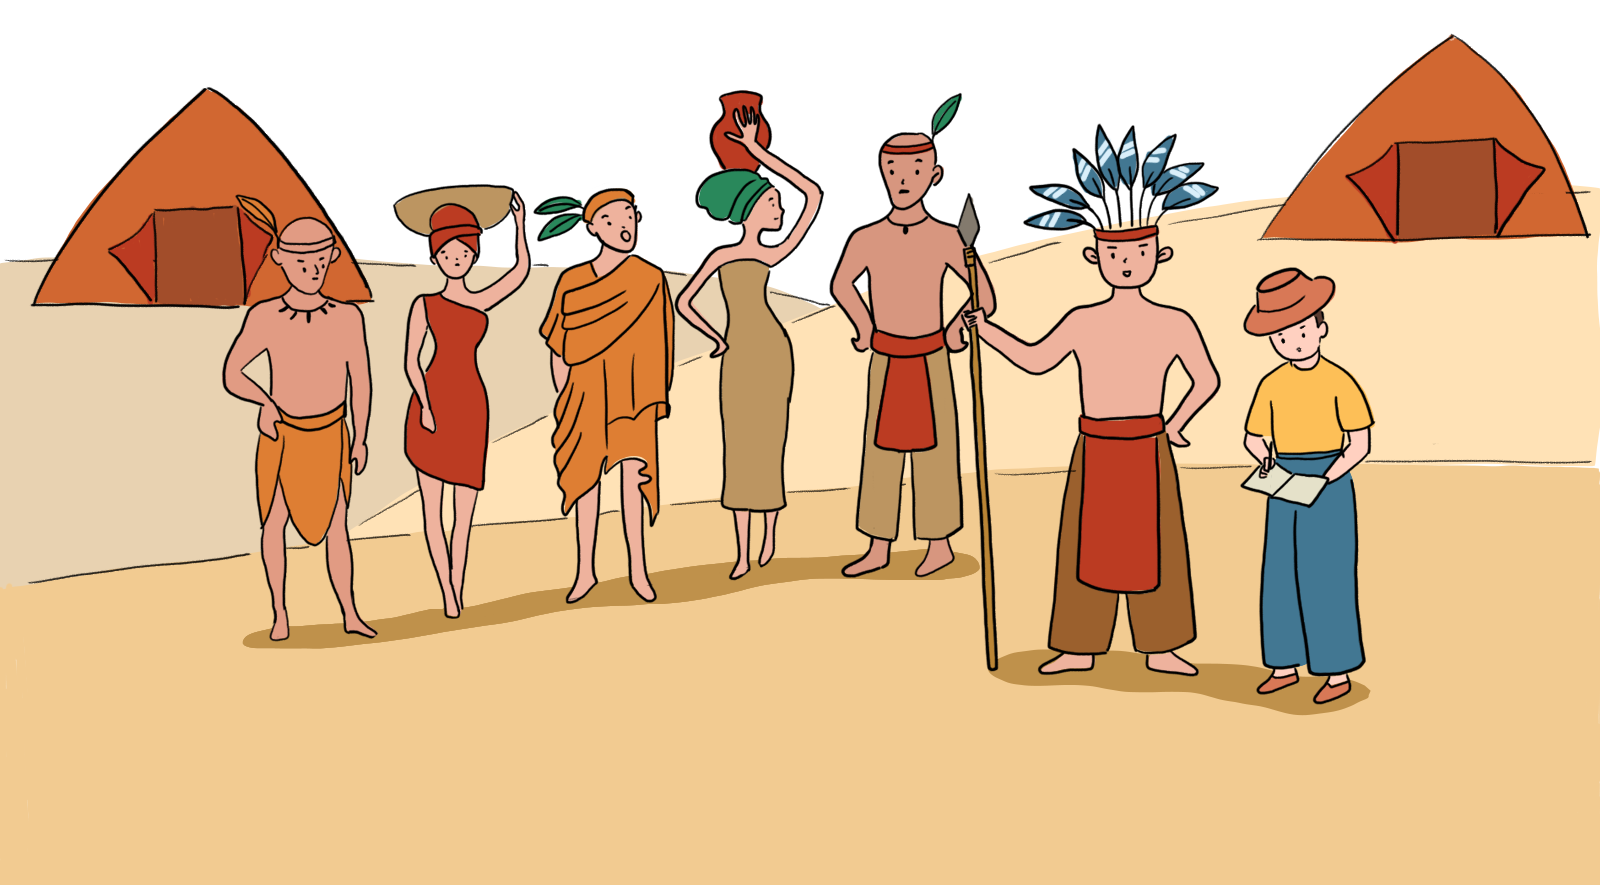
\includegraphics[width=1\linewidth]{xp}
		\vspace*{-15pt}
	\end{figure}
	Theo quy định của Hiệp hội Thương gia dành cho những người ngoài, qua lời của bà lão, Thám tử có thể đứng dậy bước tới một nơi bất kỳ nào đó trong căn phòng và chỉ được hỏi câu hỏi ``Khoảng cách từ chỗ tôi đứng đến người nói dối gần nhất trong số các anh là bao nhiêu?" cho tất cả những người trong phòng. Sau đó, mỗi người trong số $10$ người ngồi xung quanh bàn sẽ trả lời Thám tử, lúc này đã cải trang thành một Thương gia muốn gia nhập Hiệp hội. Thám tử không được phép đứng lên mặt bàn và tất cả mọi người, kể cả Thám tử, đều được phép dùng thước để đo khoảng cách tuỳ ý. Ta cũng được biết rằng ngoài $10$ người và Thám tử, trong phòng không còn có người lạ nào khác, hơn nữa $10$ người đều biết rõ ai trong số họ là nói thật và ai trong số họ là nói dối. Em hãy cho biết Xuân Phong có thể sử dụng ít nhất bao nhiêu câu hỏi như trên để biết chắc chắn ai trong số những người ngồi quanh bàn là nói~dối?
\end{multicols}
\newpage
\begingroup
\AddToShipoutPicture*{\put(115,670){
\includegraphics[scale=1]{../tieude11.pdf}}} 
\centering
\endgroup
\vspace*{35pt}

\begin{multicols}{2}
	$\pmb{1.}$ Tuấn và Tú cùng tham gia một giải thi đấu cờ vua cùng các bạn học sinh khác trong trường. Hai bạn tổng cộng ghi được $6{.}5$ điểm, trong khi tất cả các bạn học sinh còn lại đều ghi được số điểm bằng nhau. Hỏi có tất cả bao nhiêu học sinh tham gia giải cờ vua đó? (Biết rằng trong giải thi đấu, mỗi người tham gia thi đấu đúng một ván với mỗi người còn lại, ghi được $1$ điểm sau mỗi trận thắng, $0{.}5$ điểm sau mỗi trận hoà và $0$ điểm sau mỗi trận thua).
	\begin{figure}[H]
		\centering
		\vspace*{-5pt}
		\captionsetup{labelformat= empty, justification=centering}
		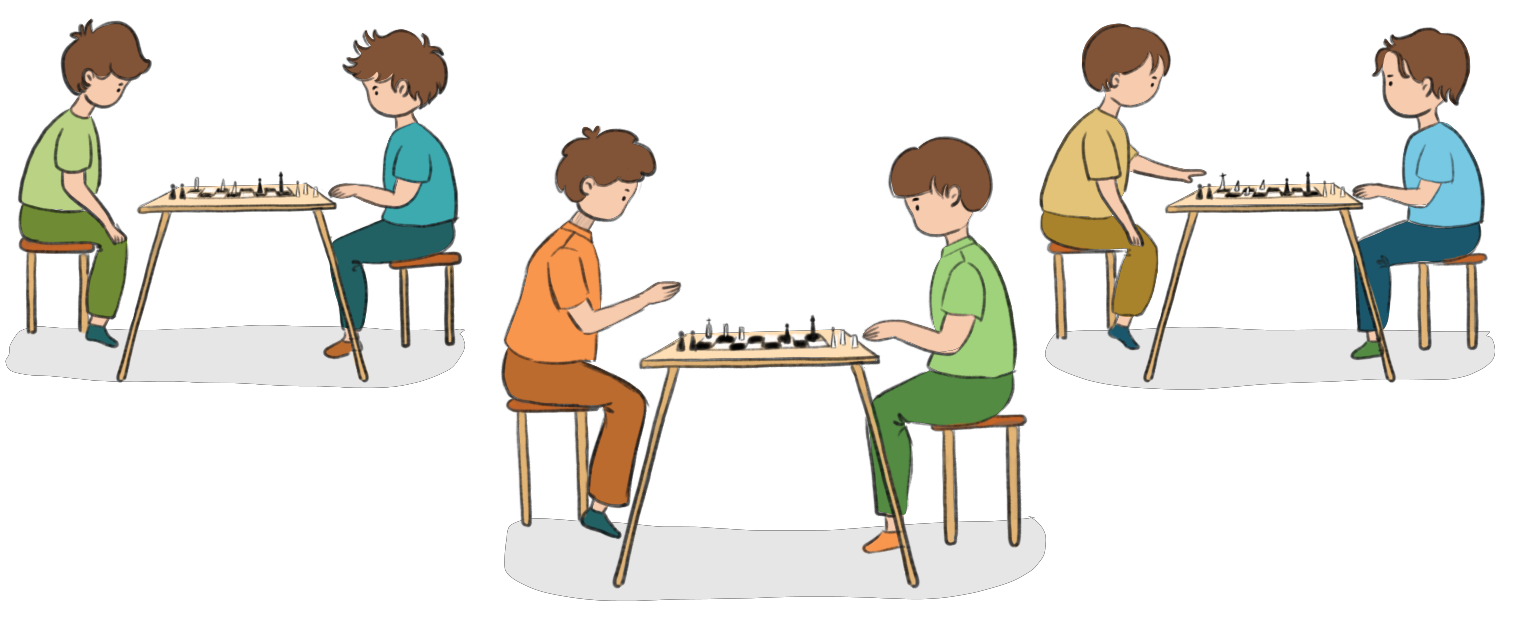
\includegraphics[width=1\linewidth]{Hinh1}
		\vspace*{-20pt}
	\end{figure}
	$\pmb{2.}$ 	Lớp $6$A gồm $22$ bạn chia thành hai đội: Xanh gồm các bạn nam và Đỏ gồm các bạn nữ để tổ chức thi tài đối đáp, trả lời thông minh. Đầu tiên, bạn Hoa ở nhóm Đỏ đối đáp với $6$ bạn nam ở nhóm Xanh và giành chiến thắng. Tiếp theo, bạn Mai ở nhóm Đỏ đối đáp với $7$ bạn nam ở nhóm Xanh và cũng giành chiến thắng. Tiếp tục bạn Huệ ở nhóm Đỏ cũng chiến thắng $8$ bạn nam ở nhóm Xanh. Cứ tiếp tục như vậy, cuối cùng bạn Hà ở nhóm Đỏ đã đối đáp thông minh với toàn bộ các bạn nam ở nhóm Xanh và giành chiến thắng chung cuộc. Hỏi trong lớp có tất cả bao nhiêu bạn nam?
	\begin{figure}[H]
		\centering
		\vspace*{-5pt}
		\captionsetup{labelformat= empty, justification=centering}
		
\includegraphics[width=1.01\linewidth]{Hinh2}
		\vspace*{-5pt}
	\end{figure}
	$\pmb{3.}$ 	Có bốn chủ doanh nghiệp tới thăm trường học cũ của mình, mang theo một số món quà với dự định sẽ trao tặng cho các học sinh đang học ở đó. Khi tất cả $252$ em học sinh được mời xếp thành một hàng ngang, chủ doanh nghiệp thứ nhất tặng quà cho mỗi em đứng thứ tư trong hàng (các em ở số thứ tự $4,8,12,$ \ldots). Chủ doanh nghiệp thứ hai lại tặng quà cho mỗi em đứng thứ bảy (các em ở số thứ tự $7,14,21$, \ldots). Chủ doanh nghiệp thứ ba trao tặng quà cho mỗi em đứng thứ mười một (các em ở số thứ tự $11,22,33$, \ldots). Chủ doanh nghiệp thứ tư sẽ tặng quà cho các em còn lại. Hỏi có bao nhiêu em học sinh nhận được quà từ mỗi chủ doanh nghiệp?
	\begin{figure}[H]
		\centering
		\vspace*{-5pt}
		\captionsetup{labelformat= empty, justification=centering}
		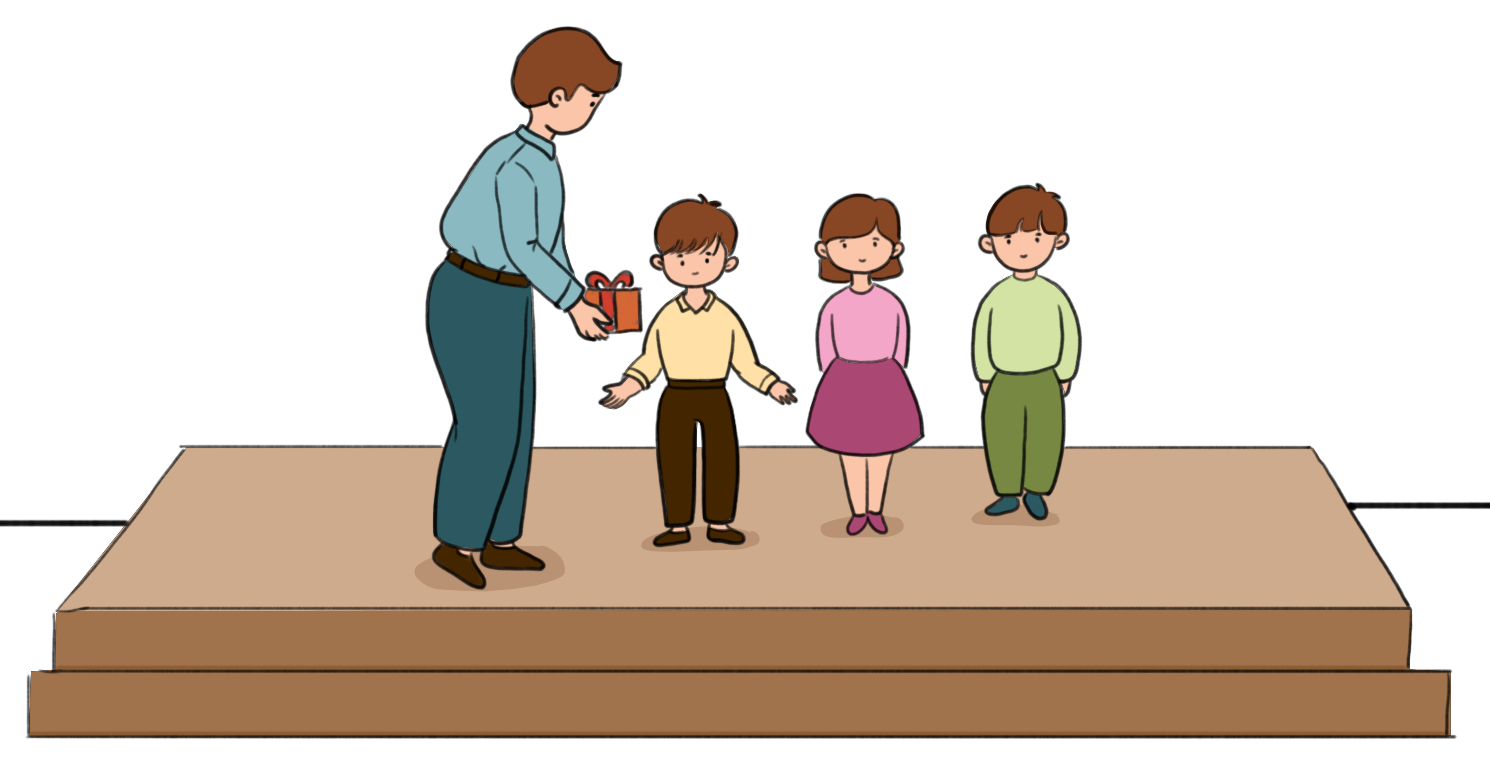
\includegraphics[width=1\linewidth]{Hinh3}
		\vspace*{-15pt}
	\end{figure}
	$\pmb{4.}$ 	Có ba nhà tài trợ quyết định giúp đỡ một tạp chí khoa học thường thức với tên gọi là Phi. Nhà tài trợ Quốc trao tặng một khoản tiền tính bằng dollar gồm có $4$ chữ số: $2$ chữ số đứng trước dấu phẩy, và hai chữ số sau dấu phẩy, trong đó số cent lẻ (tức là hai chữ số đứng sau dấu phẩy) bằng với đúng số dollar chẵn (tức là hai chữ số đứng trước dấu phẩy; ta nhớ lại $100$ cent $= 1$ dollar). Nhà tài trợ Minh tặng số tiền với số dollar chẵn lớn hơn $3$ dollar so với số dollar chẵn mà nhà tài trợ Quốc đã tặng nhưng số cent lẻ lại ít hơn $8$ lần số cent lẻ của nhà tài trợ Quốc. Nhà tài trợ Vũ hào phóng đem tặng số tiền bằng $1/7$ tổng số tiền của hai nhà tài trợ Quốc và Minh đã trao cộng lại. Hỏi số tiền ủng hộ của ba nhà tài trợ cho tạp chí Phi là bao nhiêu?
	\begin{figure}[H]
		\centering
%		\vspace*{-5pt}
		\captionsetup{labelformat= empty, justification=centering}
		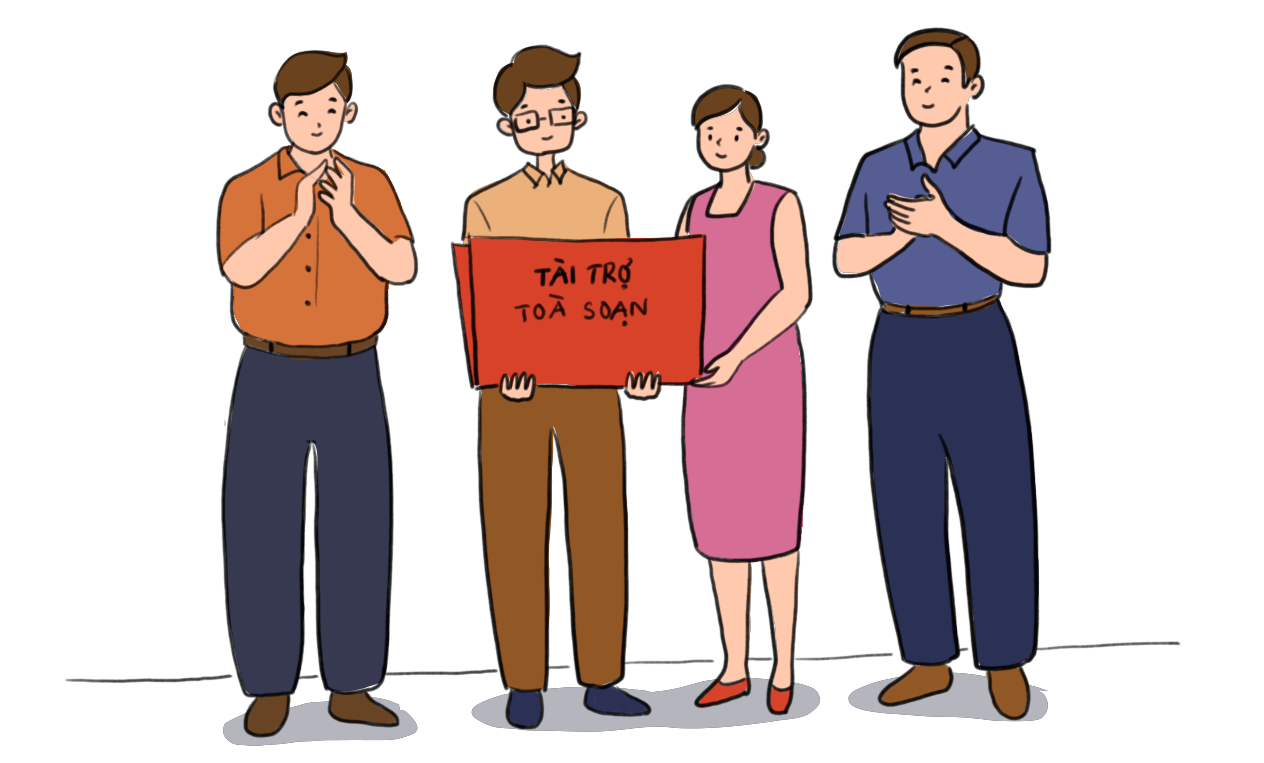
\includegraphics[width=0.8\linewidth]{Hinh4}
		\vspace*{-10pt}
	\end{figure}
	\vskip 0.1cm
	$\pmb{5.}$ 	Trên hòn đảo Ngọc ở giữa một đại dương xanh ngắt có $100$ thổ dân sinh sống, một số người trong họ luôn nói dối, còn những người còn lại luôn nói thật. Mỗi một thổ dân thờ phụng đúng một trong ba vị thần: thần Mặt trời, thần Mặt trăng hoặc thần Đất. Người ta hỏi mỗi thổ dân ba câu hỏi sau đây:
	\begin{figure}[H]
		\centering
		\vspace*{-5pt}
		\captionsetup{labelformat= empty, justification=centering}
		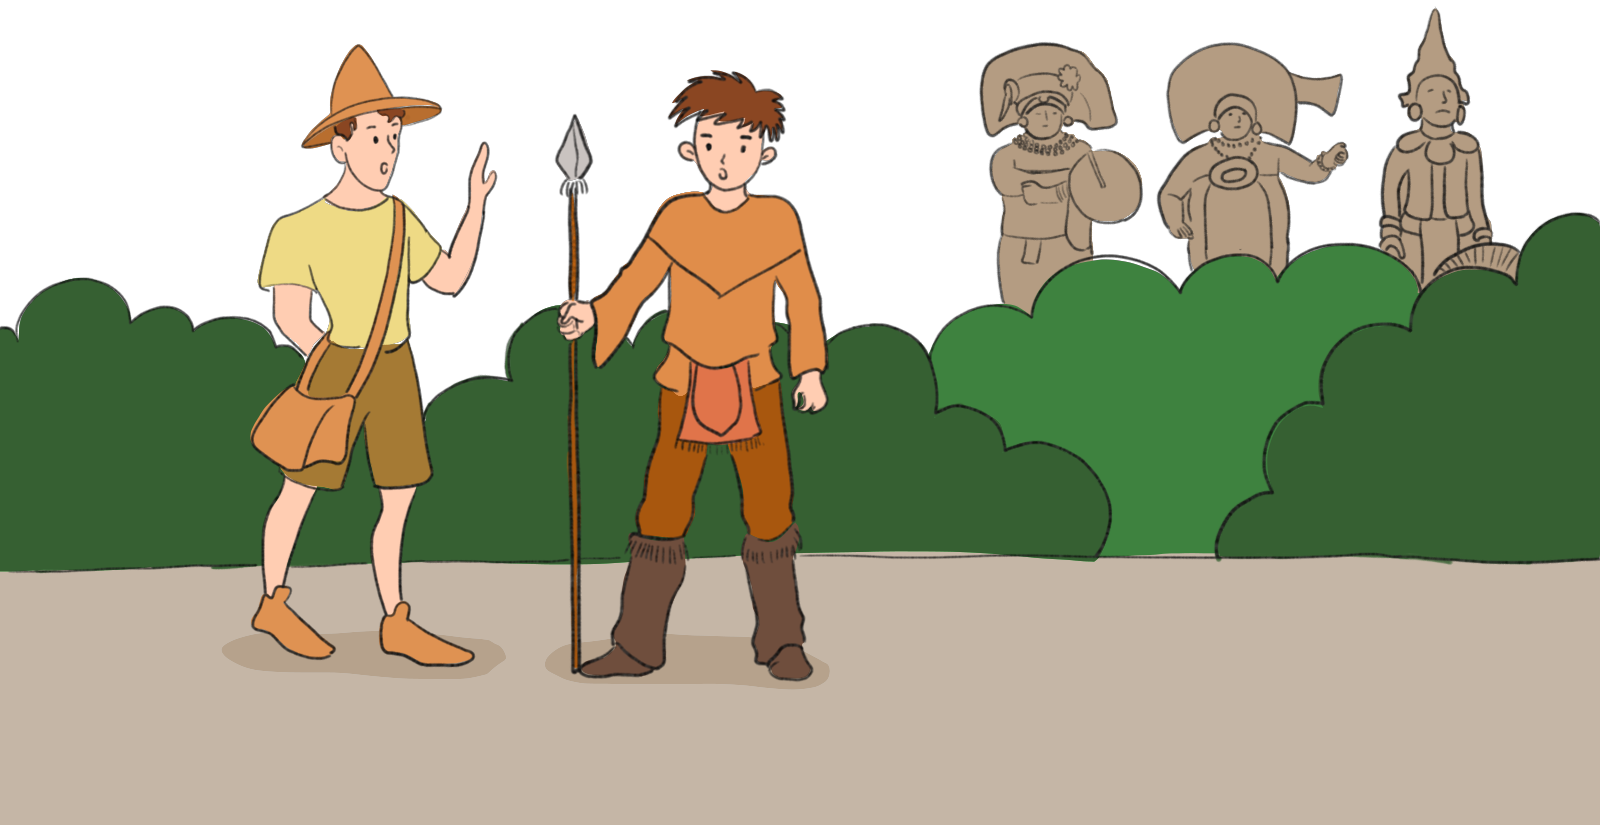
\includegraphics[width=1\linewidth]{Hinh5}
		\vspace*{-20pt}
	\end{figure}
	$1.$ Ông (bà) có thờ phụng thần Mặt trời hay không?
	\vskip 0.1cm
	$2.$ Ông (bà) có thờ phụng thần Mặt trăng hay không?
	\vskip 0.1cm
	$3.$ Ông (bà) có thờ phụng thần Đất hay không?
	\vskip 0.1cm
	Có $60$ người trả lời khẳng định ``có" với câu hỏi thứ nhất, $40$ người trả lời khẳng định ``có" với câu hỏi thứ hai và $30$ người trả lời khẳng định ``có" với câu hỏi thứ ba. Hỏi trên đảo Ngọc có bao nhiêu thổ dân nói dối?
	\vskip 0.1cm
	$\pmb{6.}$ 	Có $100$ em học sinh được mời tới buổi tổng kết cuối năm học của nhà trường. Các ghế trong phòng họp được xếp ngay ngắn thẳng hàng theo dạng một hình vuông với $10$ dãy ghế, mỗi dãy có đúng $10$ chiếc ghế. Buổi họp phải diễn ra muộn hơn do bị cắt điện, vì thế các em học sinh bắt đầu bàn luận trao đổi với các bạn bên cạnh về kết quả điểm trung bình của mình. Em học sinh nào thấy trong tất cả những bạn ngồi kề sát mình: bên trái, bên phải, đằng sau, đằng trước và theo các đường chéo, chỉ có tối đa một bạn có điểm trung bình cao hơn hoặc bằng điểm trung bình của  mình, sẽ tự coi mình là ``có thành tích".
	\begin{figure}[H]
		\centering
		\vspace*{-10pt}
		\captionsetup{labelformat= empty, justification=centering}
		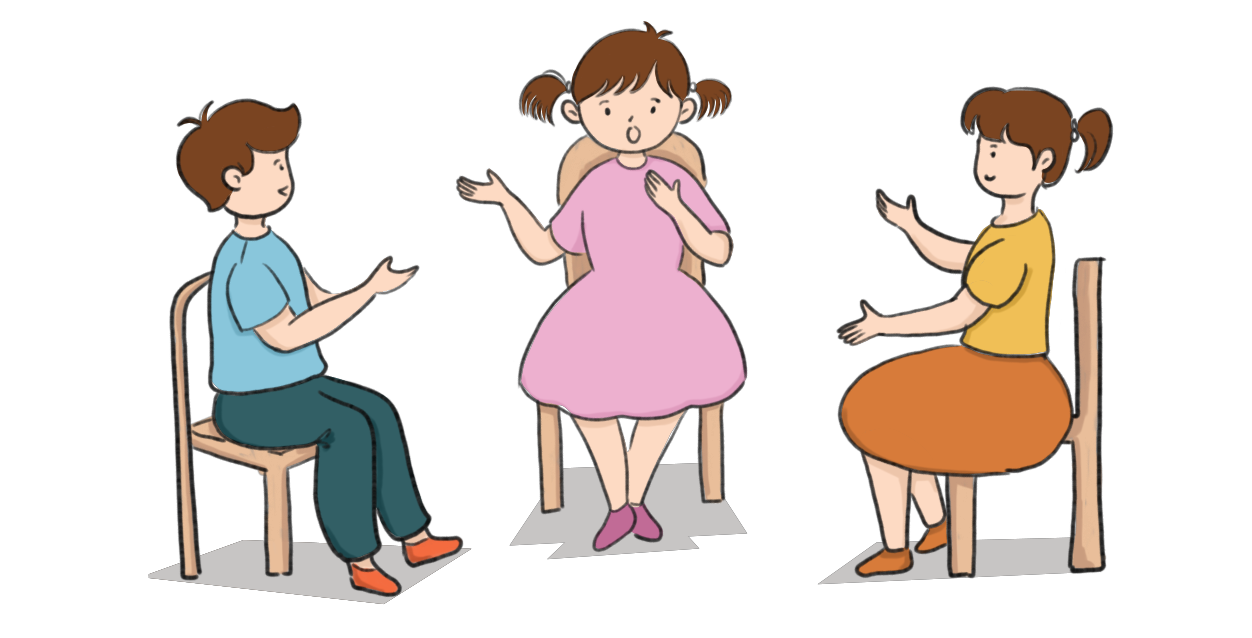
\includegraphics[width=0.85\linewidth]{Hinh6}
		\vspace*{-10pt}
	\end{figure}
	Hỏi trong buổi họp đó có thể có tối đa bao nhiêu em học sinh đã tự coi mình là ``có thành tích" trong học tập?
\end{multicols}
\vspace*{-10pt}
{\color{toancuabi}\rule{1\linewidth}{0.1pt}}
\begingroup
\AddToShipoutPicture*{\put(114,178){
\includegraphics[scale=1]{../tieude2.pdf}}} 
\centering
\endgroup
\vspace*{75pt}

\begin{multicols}{2}
	$\pmb{1.}$ Các bạn nam mang kẹo tới lớp để tặng cho các bạn nữ. Bạn Phúc nói rằng mình đã mang tới đúng một nửa tổng số kẹo. Bạn Kiên nói rằng mình đã mang tới đúng một phần ba tổng số kẹo và chỉ chia kẹo của mình cho Mai và Tuyết, hơn nữa Mai được nhiều hơn so với Tuyết là $3$ chiếc kẹo. Em hãy chứng tỏ rằng có một bạn trong số Phúc và Kiên đã \linebreak nhầm lẫn.\\
	\textit{Lời giải.} Giả sử cả hai bạn Phúc và Kiên đều không nhầm lẫn. Do Phúc không nhầm, nên tổng số kẹo được mang tới lớp phải là số chẵn (gấp $2$ lần số kẹo mà Phúc mang tới). Do Kiên cũng mang tới một số kẹo là số nguyên, bằng $1/3$ của một số chẵn, nên Kiên cũng mang tới một số kẹo là số chẵn. Theo lời của Kiên, số kẹo mà cậu đã tặng cho các bạn nữ là một số lẻ, do số kẹo mà Mai và Tuyết nhận được khác tính chẵn lẻ (hơn kém nhau là $3$ chiếc, mà $3$ là một số lẻ), mà tổng của hai số khác tính chẵn lẻ là một số lẻ. Ta nhận được mâu thuẫn. Suy ra có ít nhất một bạn nam trong số Phúc và Kiên đã nhầm lẫn.
	\begin{figure}[H]
			\centering
		\vspace*{-5pt}
		\captionsetup{labelformat= empty, justification=centering}
		
\includegraphics[width=0.6\linewidth]{Pi7_bai1}
		\vspace*{-10pt}
	\end{figure}
	$\pmb{2.}$ Ba người thợ cùng đào một chiếc hố. Họ luân phiên lần lượt làm việc, mỗi người làm việc trong một thời gian nhất định. Nếu trong khi một người làm việc hai người còn lại cũng đồng thời đào hố thì hai người này sẽ đào được đúng một nửa hố. Hỏi nếu cả ba người cùng đồng thời đào thì họ sẽ làm nhanh hơn được bao nhiêu lần so với cách làm luân phiên ban đầu?
	\begin{figure}[H]
		\centering
		\vspace*{-5pt}
		\captionsetup{labelformat= empty, justification=centering}
		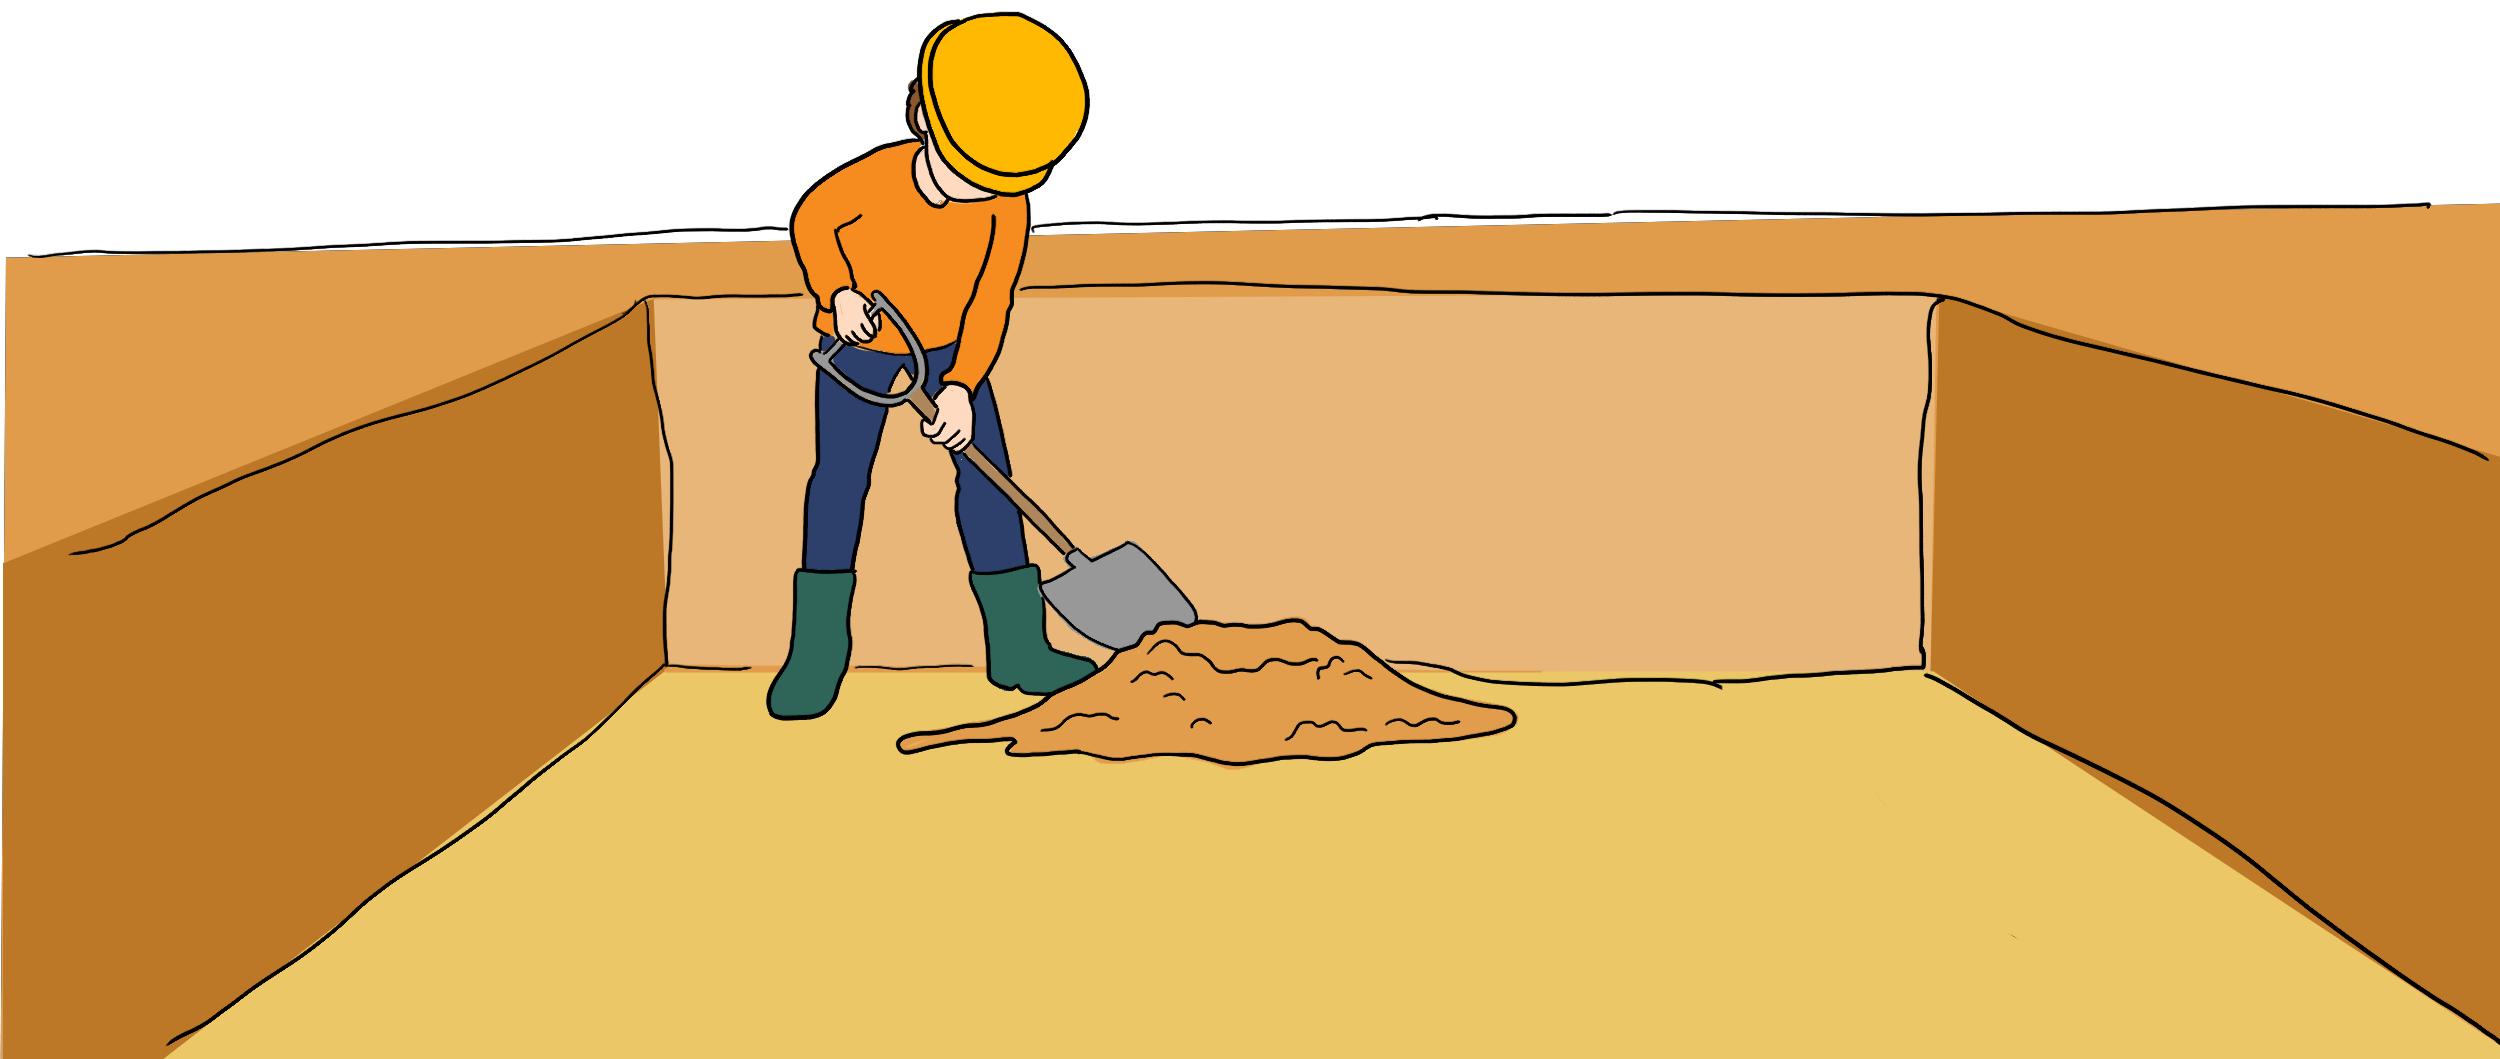
\includegraphics[width=1\linewidth]{Pi7_bai2}
		\vspace*{-20pt}
	\end{figure}
	\textit{Lời giải.} 	Giả sử trong thời gian mỗi người đào ở chiếc hố ban đầu, hai người còn lại sẽ đi đào một chiếc hố bổ sung thêm khác. Như vậy khi kết thúc công việc, cùng với chiếc hố ban đầu, họ sẽ đào thêm được $3\cdot 0{.}5 = 1{.}5$ chiếc hố. Do đó, nếu cả ba người cùng làm công việc đào, thì trong cùng số thời gian như ban đầu, họ sẽ đào được $1+1{.}5=2{.}5$ (hố). Vậy, nếu cả ba người cùng đào thì họ sẽ làm nhanh hơn được $2{.}5$ lần so với cách đào luân phiên lần lượt như ban đầu.
	\vskip 0.1cm
	$\pmb{3.}$ Ba bạn Gấu, Thỏ và Mèo cùng quyết định xây một con đường từ nhà tới bờ suối với chiều dài $160m$. Các bạn thoả thuận sẽ đầu tư cho dự án mở đường quan trọng này với công sức đều như nhau. Cuối cùng khi dự án hoàn thành, hoá ra bạn Thỏ đã xây được $60$ mét đường, bạn Mèo xây được $100$ mét đường, còn bạn Gấu mải ngủ đông nên không xây được mét nào. Tuy nhiên, Gấu mang tới đóng góp bằng tiền cho dự án là $16$ triệu đồng từ số mật ong bán được của mình. Hỏi hai bạn Mèo và bạn Thỏ cần phải phân chia số tiền cho nhau như thế nào?
	\begin{figure}[H]
		\centering
		\vspace*{-5pt}
		\captionsetup{labelformat= empty, justification=centering}
		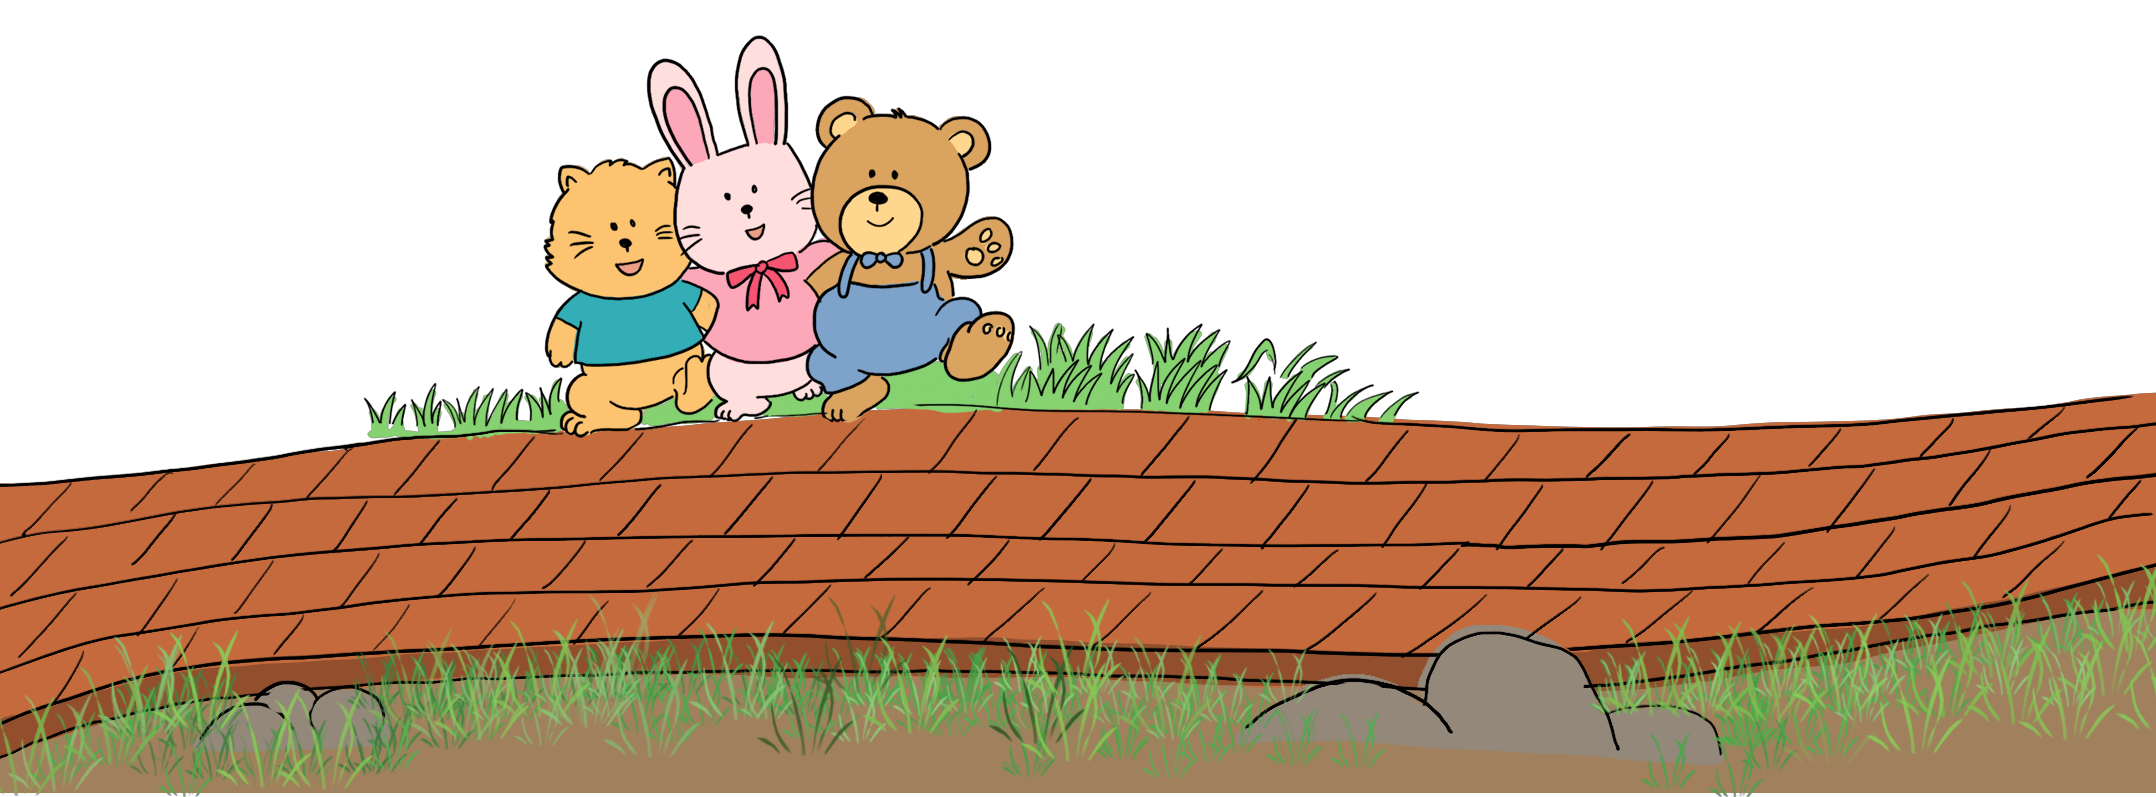
\includegraphics[width=1\linewidth]{Pi7_bai3}
		\vspace*{-15pt}
	\end{figure}
	\textit{Lời giải.} 	Mỗi bạn theo kế hoạch phải xây đúng $\dfrac{160}{3} = 53\dfrac{1}{3}$  mét đường. Thỏ xây được $60$ (m) và Gấu xây được $100$ (m). Như vậy bạn Thỏ đã xây thay cho bạn Gấu số mét đường là
	\begin{align*}
		60 - 53 \frac{1}{3} = 6 \frac{2}{3}= \frac{20}{3} \text{ (m)},
	\end{align*}
	còn bạn Mèo đã xây thay cho bạn Gấu số mét đường
	\begin{align*}
		100- 53 \frac{1}{3} = 46 \frac{2}{3}=\frac{140}{3} \text{ (m).}
	\end{align*}
	Vì vậy số tiền mà bạn Gấu mang tới phải chia cho Thỏ và Mèo theo tỷ lệ $2: 14$, tức là Mèo được $14$ triệu đồng, còn Thỏ được $2$ triệu đồng từ số tiền đóng góp công sức của Gấu.
	\vskip 0.1cm
	$\pmb{4.}$ Bé Ly phải đi trồng hoa vào một hàng các chậu rất dài đặt thành hàng dọc ở công viên. Bé được giao nhiệm vụ là phải trồng hai loại hoa khác nhau vào hai chiếc chậu nếu giữa hai chậu này có đúng hai chiếc chậu, hoặc đúng ba chiếc chậu, hoặc đúng năm chiếc chậu khác. Hỏi bé Ly phải cần ít nhất bao nhiêu loại hoa để thực hiện được nhiệm vụ?
	\begin{figure}[H]
		\centering
		\vspace*{-5pt}
		\captionsetup{labelformat= empty, justification=centering}
		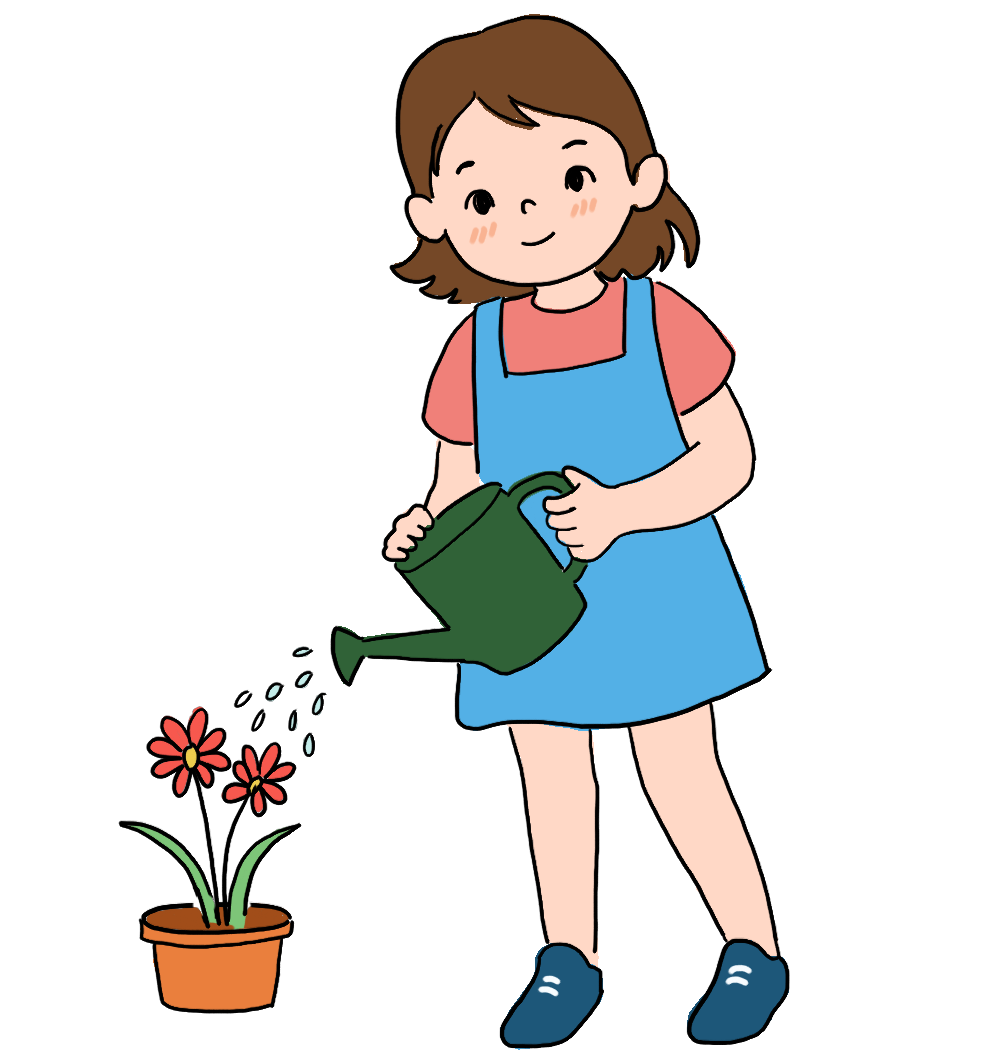
\includegraphics[width=0.45\linewidth]{Pi7_bai4}
		\vspace*{-10pt}
	\end{figure}
	\textit{Lời giải.} Trước tiên ta thấy rằng bé Ly có thể chỉ cần $3$ loại hoa là thực hiện được nhiệm vụ. Thật vậy, giả sử Ly có $3$ loại là $A, B, C$. Khi đó nếu Ly trồng $3$ chậu đầu tiên trong hàng bằng loại $A$, $3$ chậu tiếp theo bằng loại $B$, $3$ chậu tiếp loại $C$ và lại $3$ chậu tiếp theo quay lại bằng loại $A$, vv \ldots thì rõ ràng yêu cầu đặt ra được thực hiện. 
	\vskip 0.1cm
	Bây giờ giả sử Ly chỉ có $2$ loại hoa là $A$ và $B$. Nếu Ly trồng ở chậu thứ nhất bằng hoa loại $A$ (không mất tính tổng quát), suy ra các chậu có số thứ tự tiếp theo là $4, 5, 7$ phải được trồng bằng hoa loại $B$. Nhưng khi đó giữa hai chậu số $4$ và số $7$ đều được trồng cùng loại hoa $B$ nhưng giữa chúng có đúng hai chậu khác là số $5$ và số $6$, suy ra mâu thuẫn với yêu cầu.
	\vskip 0.1cm
	Vậy Ly cần ít nhất $3$ loại hoa để trồng theo yêu cầu đặt ra.
	 \vskip 0.1cm
	$\pmb{5.}$ Trước một trận bóng đá giữa hai đội Xóm Đông và Xóm Bắc có $5$ dự đoán kết quả được đưa ra:
	\vskip 0.1cm
	$a)$	Sẽ không có tỷ số hoà;
	\vskip 0.1cm
	$b)$	Đội Xóm Đông sẽ bị thủng lưới;
	\vskip 0.1cm
	$c)$	Đội Xóm Bắc sẽ thắng;
	\vskip 0.1cm
	$d)$	Đội Xóm Bắc sẽ không thua;
	\vskip 0.1cm
	$e)$	Trong trận bóng sẽ có đúng $3$ bàn thắng được ghi.
	\vskip 0.1cm
	Sau khi trận bóng kết thúc, hoá ra chỉ có đúng $3$ dự đoán là chính xác. Vậy trận đấu đã kết thúc với tỷ số như thế nào?
	\begin{figure}[H]
		\centering
%		\vspace*{-5pt}
		\captionsetup{labelformat= empty, justification=centering}
		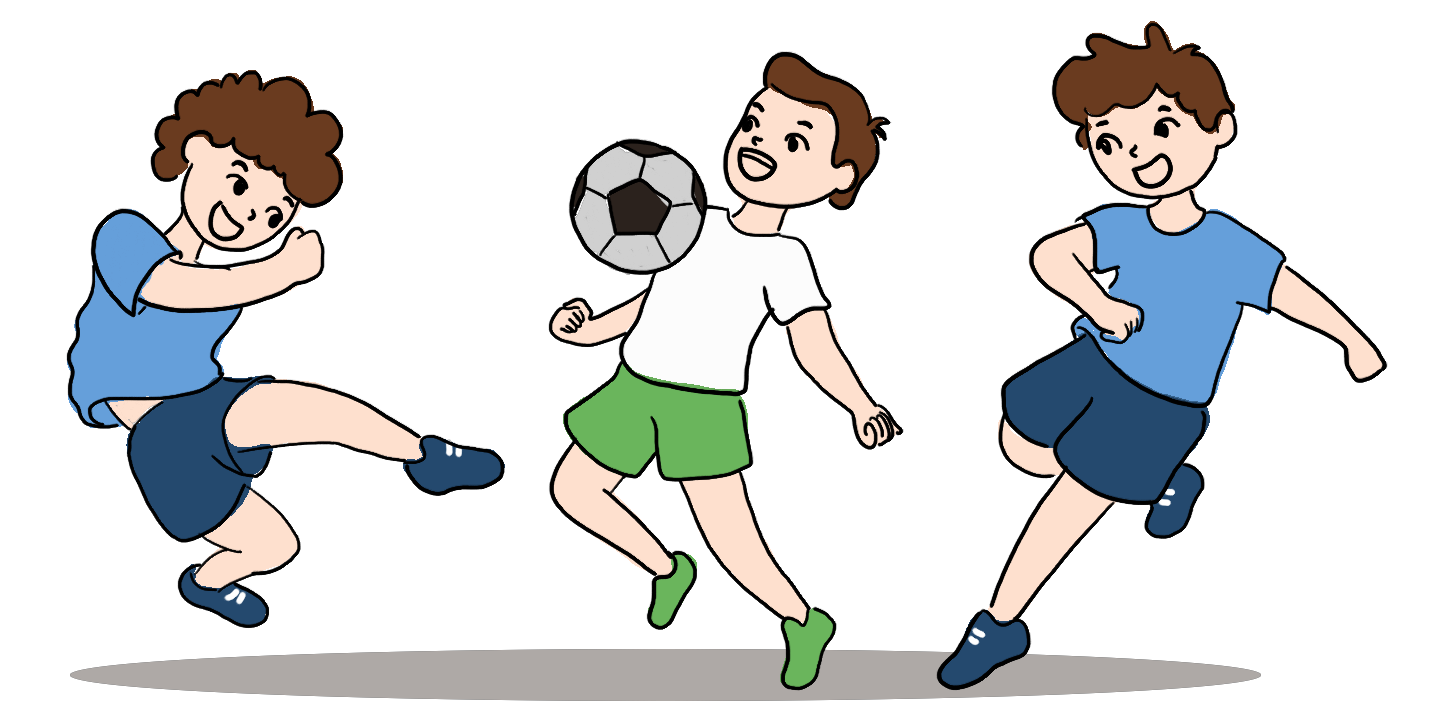
\includegraphics[width=0.85\linewidth]{Pi7_bai5}
		\vspace*{-10pt}
	\end{figure}
	\textit{Lời giải.} Giả sử là đội Xóm Bắc thắng. Khi đó $4$ dự đoán $a)$, $b)$ $c)$ và $d)$ đều đúng, mâu thuẫn với điều kiện đặt ra.
	\vskip 0.1cm
	Tiếp theo, giả sử trận đấu kết thúc với tỷ số hoà. Khi đó ta lại có các dự đoán $a)$, $c)$ và $e)$ đều sai, điều này cũng mâu thuẫn với điều kiện đã cho.
	\vskip 0.1cm
	Vì vậy, trong trận bóng này đội Xóm Bắc đã thua. Khi đó các dự đoán $c)$ và $d)$ đều sai, và $3$ dự đoán còn lại là đúng. Có nghĩa là: trận đấu không có tỷ số hoà, có ít nhất một trái bóng được đưa vào lưới của đội Xóm Đông, và trong trận bóng có đúng $3$ bàn thắng được ghi. Điều đó có nghĩa là trận bóng kết thúc với tỷ số $1:2$ nghiêng về phía đội Xóm Đông.
	\vskip 0.1cm
	$\pmb{6.}$ 	Tại trại hè có $20$ em học sinh tham gia trò chơi Điệp viên tí hon diễn ra trong $2$ tuần. Mỗi Điệp viên tí hon sẽ theo dõi và viết báo cáo tỉ mỉ về sở thích cá nhân của $10$ em khác trong số $20$ em này để nộp cho Sở chỉ huy. Em hãy chứng tỏ rằng có ít nhất $10$ cặp Điệp viên tí hon đã theo dõi lẫn nhau và viết báo cáo về nhau.
	\begin{figure}[H]
		\centering
		\vspace*{-5pt}
		\captionsetup{labelformat= empty, justification=centering}
		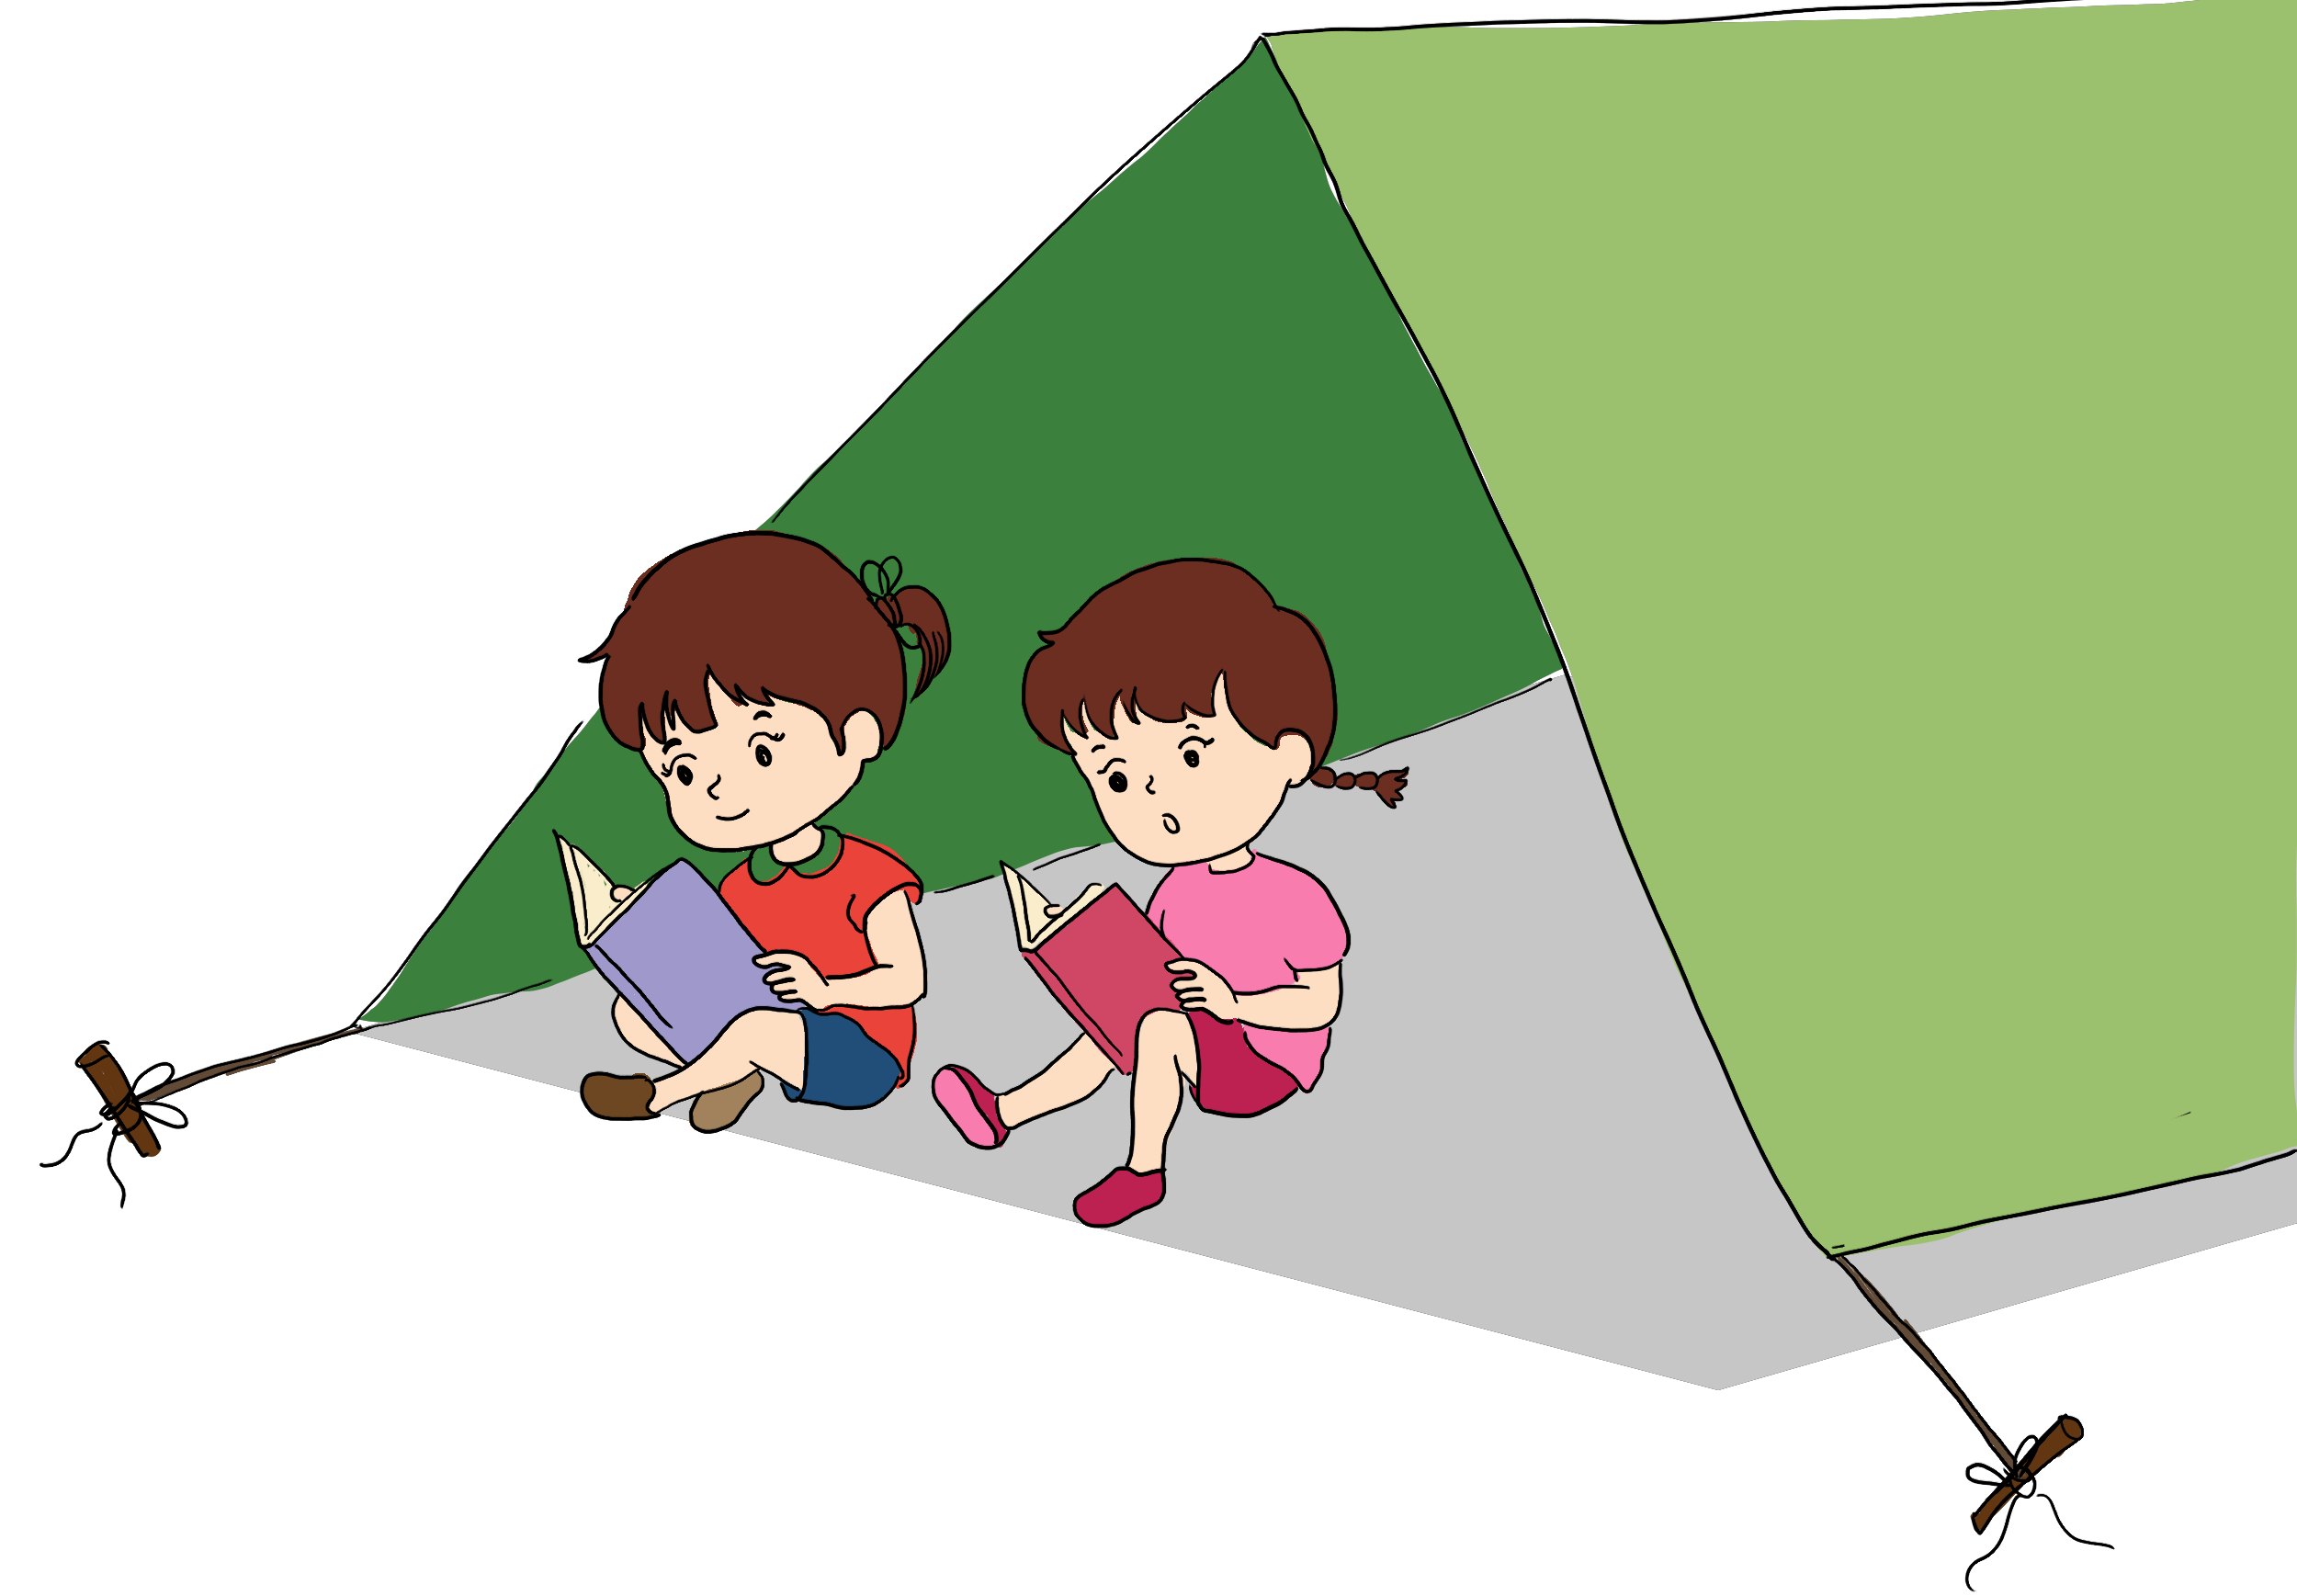
\includegraphics[width=0.75\linewidth]{Pi7_bai6}
		\vspace*{-15pt}
	\end{figure}
	\textit{Lời giải.} Số các cặp Điệp viên tí hon là $\dfrac{20\times 19}{2} = 190$ (cặp). Có tất cả $10\times 20=200$ báo cáo được gửi về Sở chỉ huy vào cuối đợt chơi, suy ra phải có ít nhất $10$ cặp Điệp viên mà hai người trong mỗi cặp báo cáo lẫn nhau về Sở chỉ huy.
\end{multicols}

\newpage
\begingroup
\thispagestyle{toancuabinone}
\blfootnote{$^1$\color{toancuabi}Ottawa, Canada.}
\AddToShipoutPicture*{\put(60,733){
\includegraphics[width=17.2cm]{../mathc.pdf}}}
%\AddToShipoutPicture*{\put(-2,733){
\includegraphics[width=17.2cm]{../mathl.pdf}}} 
\AddToShipoutPicture*{\put(110,675){
\includegraphics[scale=1]{../tieudeb.pdf}}} 
\centering
\endgroup
\vspace*{35pt}

\begin{multicols}{2}
	In this article, we discuss the Extremal Principle and its applications.
	One of the simplest forms of the principle is as follow:
	``in a finite set of numbers, there is a number with minimal value,
	i.e. it is smaller than or equal to any other number in the set.
	Similarly there is a number with maximal value,
	i.e. it is larger than or equal to any other number in the set."
	\vskip 0.1cm
	\textit{Proof by contradiction} is an extremely useful tool when combining with the Extremal Principle,
	as you will see in below examples.
	\vskip 0.2cm
	\PIbox{{\color{toancuabi}\textbf{\color{toancuabi}Example} (Dancing at a party)}
			At a party no boy danced with all the girls,
			but each girl dances with at least one boy.
			Prove that there are two pairs of girl--boy $(g_1, b_1)$ and $(g_2, b_2)$
			who danced with each other but $g_1$ did not dance with $b_2$
			and $g_2$ did not dance with $b_1.$}
	\vskip 0.2cm
	\textit{Solution.}
		Let $b_1$ be \textit{the boy who danced with the maximum number of girls.}
		Then there is a girl $g_2$ who he did not danced with.
		For $g_2$ there is a boy $b_2$ that $(g_2,b_2)$ danced together.
		Among the girls who danced with $b_1$ there is at least one $g_1$ who did not danced with $b_2,$
		otherwise $b_2$ danced with $g_2$ and all the girls that $b_1$ danced with,
		meaning $b_2$ danced with more girls than $b_1,$ contradicting with the choice of $b_1.$
	\vskip 0.2cm
	\PIbox{{\color{toancuabi}\textbf{\color{toancuabi}Example} (Infinity by contradiction)}
			$\Omega$ is a set of points on the plane.
			Every point in $\Omega$ is a midpoint of two points in $\Omega$.
			Show that $\Omega$ is infinite set.}
	\vskip 0.2cm
	\textit{Solution.}
	Suppose that $\Omega$ is a finite set.
	According to the Extremal Principle,
	\textit{there exists two points $A, B \in \Omega,$ such that the distance $AB$ is maximal.}
	\vskip 0.1cm
	Now, since $B \in \Omega,$ there exist two points $C,D \in \Omega$ so that $B$ is the midpoint of $CD.$
	\begin{figure}[H]
			\vspace*{-5pt}
			\centering
			\captionsetup{labelformat= empty, justification=centering}
			\begin{tikzpicture}[toancuabi,scale=0.75]
					\draw  (0.,0.)-- (3.,3.);
					\draw  (3.,3.)-- (5.,-3.);
					\draw  (5.,-3.)-- (0.,0.);
					\draw  (0.,0.)-- (4.,0.);
						\draw [fill=white] (0.,0.) circle (1.5pt);
						\draw (-0.32,0.11) node {$A$};
						\draw [fill=white] (3.,3.) circle (1.5pt);
						\draw (3.14,3.37) node {$C$};
						\draw [fill=white] (5.,-3.) circle (1.5pt);
						\draw (5.32,-3.01) node {$D$};
						\draw [fill=white] (4.,0.) circle (1.5pt);
						\draw (4.36,0.15) node {$B$};
				\end{tikzpicture}
			\vspace*{-10pt}
		\end{figure}    
	Since one of the angles $\angle ABC,$ $\angle ABD,$ says $\angle ABD$ is at least $90^{\circ},$
	thus in $\triangle ABD,$ $AD > AB.$
	This contradicts the assumption that $A, B$ are the two points in $\Omega,$ such that the distance $AB$ is maximal.
	\vskip 0.1cm	
	Thus, there are no such two points $A, B,$ so $\Omega$ is infinite set.
	\vskip 0.2cm
	\PIbox{{\color{toancuabi}\textbf{\color{toancuabi}Example} (How many olives did the knights eat?)}
		At the dinner of King Anthony, several knights sits around a round table eating green olives.
		Minh, the Magician, made sure that each knight ate either twice as many olives
		or $10$ olives less than his right neighbour. 
		Is that possible that the knights could have eaten exactly $1001$ olives?}
	\vskip 0.2cm
	\textit{Solution.}
	Let assume that the knights have eaten exactly $1001$ olives.
	Let choose the knight who \textit{ate the smallest number of olives}.
	(If there are some of them, choose one.)
	His neighbour on the left, knight $k$, ate either $10$ less or twice more.
	Since the knight we chose ate the smallest number of olives, then knight $k$ ate twice as many.
	Therefore, knight $k$ ate an even number of olives. 
	\vskip 0.1cm	
	The neighbour on the left of knight $k$ ate either twice as many olives or $10$ olives less,
	hence he ate an even number of olives as well. Making the full circle, we'll end us with the first knight,
	who must have eaten an even number of olives as well.
	\vskip 0.1cm	
	Therefore, the total number of olives must be an even number.
	The number of olives eaten cannot be $1001.$
	\vskip 0.2cm
	\PIbox{{\color{toancuabi}\textbf{\color{toancuabi}Example} (Chop the flies)}
		$25$ flies are resting on the outdoor table in the garden, waiting for lunch to be served.
		It is known that for any three of them, two are at a distance less than $20$ cm;
		and there are at least a pair of flies that are further than $20$ cm from each other.
		\vskip 0.1cm
		Minh's mother gave him a fly swatter, shown below, with a hoop of radius $20$ cm,
		With a single strike he can swat the flies where the hoop landed.
		In \textit{at least} how many strikes can he swat all of them?
		\textit{Note that Minh is so fast that the flies do not have time for reaction during and between his lightning strikes.}}
	\vskip 0.2cm
	\textit{Solution.}
	If no $2$ flies are further than $20$ cm from each other,
	Minh can strike them all in $1$ strike by aiming the center of the swatter at any fly. 
	But this is not the case, so let’s assume there are $2$ flies, $A$ and $B$, that are more than $20$ cm apart.
	Then, every other fly is either in a $20$ cm radius of $A$ or in a $20$ cm radius of $B.$
	Out of the $23$ remaining flies either at least $12$ will be in the $20$ cm radius of $A$
	or $12$ will be in the $20$ cm radius of $B$.
	Swatting that the $A$ or $B$ fly with the center of the swatter kills at least $13$.
	\vskip 0.1cm
	Thus, by $2$ strikes, he can swat them all.
\end{multicols}

	\newpage 

	\setcounter{figure}{0}
	\thispagestyle{hoccungpinone}
\pagestyle{hoccungpi}
\everymath{\color{hoccungpi}}
\graphicspath{{../hoccungpi/pic/}}
\blfootnote{\color{hoccungpi}\color{hoccungpi}$^1$Giáo viên Toán trường THPT chuyên Lê Hồng Phong, Nam Định.}
\begingroup
\AddToShipoutPicture*{\put(0,616){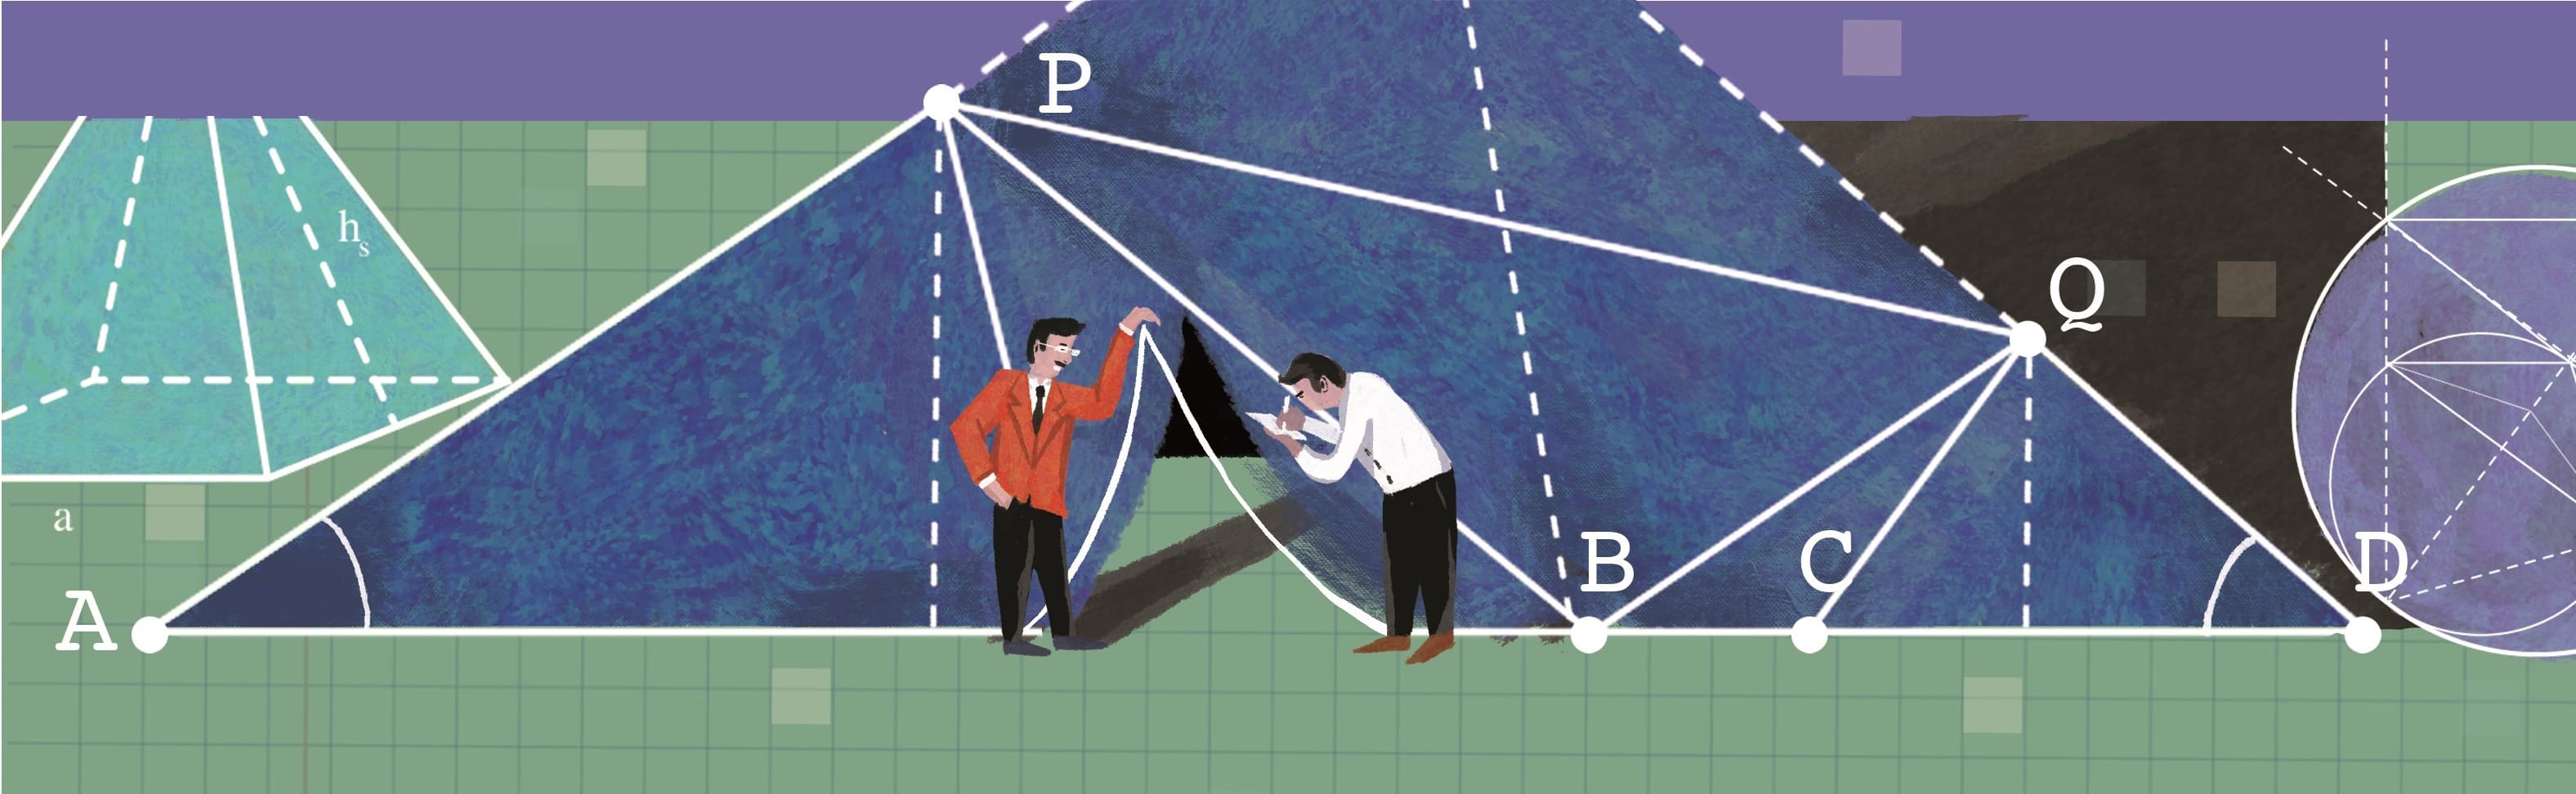
\includegraphics[width=19.3cm]{../bannerhoccungpi}}}
\AddToShipoutPicture*{\put(58,520){
\includegraphics[scale=1]{../tieude.pdf}}}
\centering
\endgroup
\vspace*{190pt}

\textit{Có thể nói rằng, sự ra đời của lý thuyết đồ thị được đánh dấu bằng bài báo \textit{bảy cây cầu ở thành phố Königsberg} của Leonhard Euler. Trải qua hàng trăm năm, lý thuyết đồ thị đã trở thành một mảng kiến thức đồ sộ, là một trong những công cụ mạnh, được sử dụng nhiều trong cả hai phân môn Toán lý thuyết và Toán ứng dụng. Trong bài viết này, chúng tôi trình bày ngắn gọn một số kiến thức cơ sở của lý thuyết đồ thị, và một số ví dụ trong việc xây dựng mô hình đồ thị. Sau đó, chúng tôi giới thiệu hai cấu trúc đồ thị đặc biệt và một số bài tập liên quan.}
\begin{multicols}{2}
	\textbf{\color{hoccungpi}Sơ lược về lý thuyết đồ thị}
	\begin{figure}[H]
		\vspace*{-5pt}
		\centering
		\captionsetup{labelformat= empty, justification=centering}
		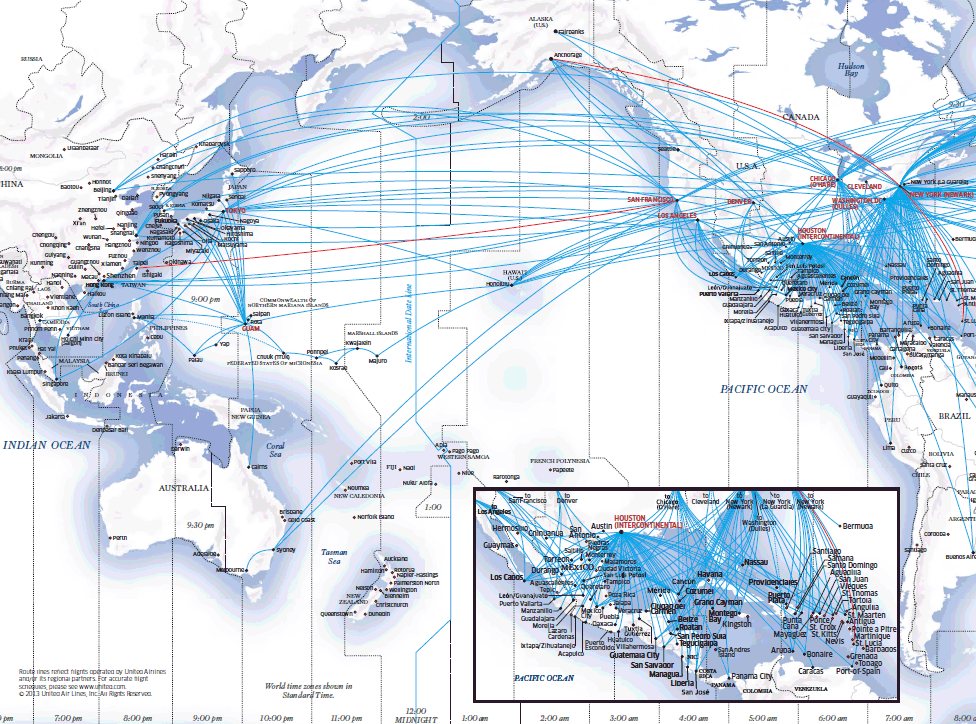
\includegraphics[width= 1\linewidth]{United_Airlines_asia_pacific}
		\caption{\small\textit{\color{hoccungpi}Hình $1$. Bản đồ các đường bay ở Châu Á -- Thái Bình Dương của hãng hàng không United Airlines.}}
		\vspace*{-10pt}
	\end{figure}
	Lý thuyết đồ thị có lịch sử phát triển lâu dài từ thế kỷ $18$. Càng ngày, người ta càng thấy nhiều ứng dụng của lý thuyết đồ thị trong nhiều lĩnh vực của cuộc sống như giao thông, y sinh, tin học, thiên văn\dots. Hình $1$\footnote[2]{\url{https://www.airlineroutemaps.com/maps}} là bản đồ các tuyến đường bay của hãng hàng không United Airlines ở khu vực Châu Á -- Thái Bình Dương.
	\vskip 0.1cm
	Trong hình này, nếu ta coi mỗi sân bay như một điểm, và mỗi đường bay như một cạnh nối hai điểm, thì đây chính là một mô hình bao gồm hai tập hợp: tập hợp điểm, và tập hợp cạnh thể hiện mối liên hệ giữa các điểm. Trong cả lý thuyết và thực tế, đôi khi ta gặp những mô hình có thể biểu diễn thông qua mô hình hai tập hợp này. Những mô hình như vậy đều có thể coi là một mô hình đồ thị. Ta đi đến định nghĩa sau về đồ thị (vô hướng): 
	\vskip 0.1cm
	\textbf{\color{hoccungpi}Định nghĩa} $\pmb{1.1}$ (Đồ thị)\textbf{\color{hoccungpi}.}
		Một \textit{đồ thị} là một tập hợp các điểm (gọi là các \textit{đỉnh} của đồ thị), và một tập hợp các đoạn (gọi là \textit{cạnh} của đồ thị), sao cho mỗi đoạn này đều có hai đầu mút là hai đỉnh của đồ thị. 
	\vskip 0.1cm
	Theo định nghĩa $1.1$, ta thấy rằng mỗi đồ thị $\pazocal{G}$ là một bộ $(V,E)$ gồm hai tập hợp: tập đỉnh $V$ và tập cạnh $E$. Vì vậy, ta thường ký hiệu đồ thị $\pazocal{G} = (V,E)$. Ta có một số lưu ý sau:  
	\vskip 0.1cm
	$\bullet$ Mỗi đồ thị không có khuyên (cạnh tự nối), và hai đỉnh bất kỳ được nối với nhau bằng nhiều nhất một cạnh gọi là một đồ thị đơn giản, hay ngắn gọn là \textit{đồ thị đơn}. Ngược lại, đồ thị mà giữa hai đỉnh có thể có nhiều hơn một cạnh được gọi là đa đồ thị.
	\vskip 0.1cm
	$\bullet$ Trong bài viết này, khi nói đến ``đồ thị'', nếu không có lưu ý gì, ta hiểu đó là một đồ thị đơn và hữu hạn (nghĩa là tập đỉnh và tập cạnh là các tập hữu hạn).
	\vskip 0.1cm
	Ta kết thúc phần này với một số định nghĩa, và một kết quả quen thuộc\footnote[3]{\color{hoccungpi}Một số khái niệm như đường đi có thể được định nghĩa hơi khác nhau giữa các tài liệu khác nhau (chú thích của BBT).}. 
	\vskip 0.1cm
	\textbf{\color{hoccungpi}Định nghĩa} $\pmb{1.2}$ (Một số định nghĩa quan trọng)\textbf{\color{hoccungpi}.}
	\vskip 0.1cm
	$1.$ Một đỉnh của đồ thị có \textit{bậc} $n$ nếu nó là đầu mút của $n$ cạnh trong đồ thị. Ký hiệu bậc của  đỉnh $v$ là deg$(v)$. 
	\vskip 0.1cm
	$2.$ Một \textit{đường đi} trên đồ thị là một dãy các đỉnh $u_1, u_2, \dots,u_k$ sao cho giữa hai đỉnh liên tiếp $u_i,u_{i+1}$ trong dãy đều có một cạnh của đồ thị nối chúng. Đường đi trong đó mỗi đỉnh chỉ được đi qua nhiều nhất một lần gọi là \textit{đường đi đơn}.
	\vskip 0.1cm
	$3.$ Đồ thị $\pazocal{G}$ được gọi là \textit{liên thông} nếu với hai đỉnh $u,v$ tùy ý, tồn tại một đường đi từ $u$ đến $v$.
	\vskip 0.1cm
	$4.$ Một \textit{chu trình} là một đường đi mà đỉnh xuất phát trùng với đỉnh kết thúc. Chu trình đi qua tất cả các đỉnh của đồ thị, mỗi đỉnh đúng một lần  được gọi là \textit{chu trình Hamilton}. Chu trình đi qua tất cả các cạnh của đồ thị, mỗi cạnh đúng một lần được gọi là \textit{chu trình Euler}.
	\vskip 0.1cm
	$5.$ \textit{Đồ thị đầy đủ} là đồ thị mà giữa hai đỉnh bất kỳ đều có một cạnh nối. 
	\vskip 0.1cm
	$6.$ Đồ thị $G$ gọi là một \textit{đồ thị con} của đồ thị $\pazocal{G}$ nếu tập đỉnh và tập cạnh của đồ thị $G$ lần lượt là tập con của tập đỉnh và tập cạnh của đồ thị $\pazocal{G}$.
	\vskip 0.1cm
	$7.$ Một \textit{thành phần liên thông} của một đồ thị là một đồ thị con trong đó giữa bất kỳ hai đỉnh nào đều có đường đi đến nhau, và không thể nhận thêm bất kỳ một đỉnh hoặc một cạnh nào mà vẫn duy trì tính chất trên. Ta thấy ngay rằng một đồ thị bất kỳ có thể được phân tích một cách duy nhất thành hợp rời của các  thành phần liên thông. 
	\vskip 0.1cm
	\textbf{\color{hoccungpi}Bổ đề} $\pmb{1.1}$ (Bổ đề bắt tay)\textbf{\color{hoccungpi}.}
		Cho đồ thị $\pazocal{G} = (V,E)$. Khi đó:
		\begin{align*}
			\sum\limits_{v \in V} deg(v) = 2 |E|.
		\end{align*}
	Việc chứng minh bổ đề không có gì là khó khăn và ta thu được ngay một hệ quả là: số đỉnh bậc lẻ trong mọi đồ thị luôn là một số chẵn. 
	\vskip 0.1cm
	$\pmb{2.}$ \textbf{\color{hoccungpi}Phát hiện và sử dụng mô hình đồ thị}
	\vskip 0.1cm
	Kỹ năng đầu tiên cần rèn luyện khi sử dụng lý thuyết đồ thị là phát hiện được mô hình. Trong rất nhiều bài toán, ý tưởng về một mô hình đồ thị được ẩn đi một cách khéo léo. Chúng ta cùng xét một số ví dụ.
	\vskip 0.1cm
	\textbf{\color{hoccungpi}Ví dụ} $\pmb{2.1}$ (Olympic Ấn Độ năm $2023$)\textbf{\color{hoccungpi}.} Cho $\pazocal{S}$ là một tập hợp gồm hữu hạn số nguyên dương. Giả sử rằng có đúng $2023$ cặp $(x,y)$ trong $\pazocal{S} \times \pazocal{S}$, sao cho tích $xy$ là số chính phương. Chứng minh rằng có thể tìm được ít nhất bốn số phân biệt trong $\pazocal{S}$ sao cho tích của hai số bất kỳ trong bốn số này không là số chính phương.
	\vskip 0.1cm
	\textit{Lời giải.} Ta xây dựng đồ thị $\pazocal{G}$ với tập đỉnh chính là tập $\pazocal{S}$, hai đỉnh $x,y$ của nó được nối với nhau bằng một cạnh nếu $xy$ là số chính phương. Ta có nhận xét quan trọng sau: nếu $x-y$ và $y-z$ là hai cạnh của đồ thị thì $x-z$ cũng là cạnh của đồ thị. Thật vậy, nếu $xy = a^2, yz = b^2$ thì $xz = (ab)^2 / y^2$. Bạn đọc có thể chứng minh được rằng vế phải là một số chính phương, do đó $xz$ cũng là số chính phương. 
	\vskip 0.1cm
	Từ nhận xét trên, ta thấy ngay cấu trúc của đồ thị $\pazocal{G}$ là như sau: nó gồm các thành phần liên thông mà mỗi thành phần liên thông là một đồ thị đầy đủ. Từ đây, bài toán quy về chứng minh đồ thị $\pazocal{G}$ có ít nhất bốn thành phần liên thông. Thật vậy, giả sử $\pazocal{G}$ có ít hơn bốn thành phần liên thông, ta gọi số đỉnh của các thành phần liên thông này là $a_1, a_2, a_3$ (các $a_i$ có thể bằng $0$). Mỗi đồ thị (đơn) đầy đủ trên $a$ đỉnh có $\frac{a(a-1)}{2}$ cạnh, và mỗi cạnh đóng góp $2$ đơn vị vào  số cặp $(x, y)$ để $xy$ là một số chính phương. Tuy nhiên, ta chú ý rằng mỗi đỉnh tương ứng với số $s\in S$, mặc dù không nối với chính nó do tính đơn của đồ thị, nhưng thỏa mãn $ss$ là một số chính phương, nên cũng đóng góp $1$ đơn vị vào số cặp $(x, y)$ để $xy$ là một số chính phương. Chính vì vậy, mỗi thành phần liên thông trên $a$ đỉnh có $a(a-1)+a=a^2$ cặp $(x,y)$ như vậy. Suy ra số cặp $(x,y)$ trong $\pazocal{S} \times \pazocal{S}$, sao cho tích $xy$ là một số chính phương bằng
	\begin{align*}
		a_1^2 + a_2^2 + a_3^2 =2023.
	\end{align*}
	Mặt khác, một số chính phương khi chia cho $8$ có số dư thuộc tập hợp $\{0;1;4\}$. Do đó, vế trái là tổng của ba số chính phương, nên không thể chia $8$ dư $7$, trong khi đó $2023$ chia $8$ dư $7$. Điều này là mâu thuẫn!   
	\vskip 0.1cm
	\textbf{\color{hoccungpi}Ví dụ} $\pmb{2.2}$ (Bài toán dự tuyển thi IMO năm $2018$, Armenia đề xuất)\textbf{\color{hoccungpi}.}
	Queenie và Horst chơi một trò chơi trên một bàn cờ kích thước $20 \times 20$. Ban đầu, bàn cờ chưa có quân cờ nào. Ở mỗi lượt đi, Horst đặt một quân mã đen vào một ô còn trống sao cho quân mã này không thể ăn được bất cứ quân mã nào đã đặt trước đó; sau đó, Queenie đặt một quân hậu vào một ô trống tùy ý. Trò chơi kết thúc khi một trong hai người không thể đặt thêm quân lên bàn cờ. Tìm số nguyên dương $K$ lớn nhất sao cho với mọi chiến thuật chơi của Queenie, Horst có thể đặt được ít nhất $K$ quân mã lên bàn cờ.  
	\vskip 0.1cm
	\textit{Lời giải.}
	Ta chỉ ra giá trị lớn nhất của $K$ là $K=100$ qua hai bước. Đầu tiên, ta chỉ ra một chiến lược mà Host có thể đặt được ít nhất $100$ quân mã lên bàn cờ. Sau đó, ta chỉ ra một chiến lược của Queenie mà Horst không thể đặt quá $100$ quân mã lên bàn cờ.
	\vskip 0.1cm
	\textbf{\color{hoccungpi}Chiến lược của Horst.} Ta tô màu đen, trắng các ô của bàn cờ một cách đan xen như bàn cờ vua thông thường. Horst chỉ cần lần lượt đặt các quân mã lên một ô đen còn trống. Để ý rằng bàn cờ có $20\cdot 20/2 = 200$ ô đen và hai con mã ở hai ô cùng màu không thể ăn nhau. Do sau mỗi lượt đi, số ô đen còn trống giảm đi không quá $2$ nên trò chơi chỉ kết thúc sau ít nhất $100$ lượt đi và vì thế Horst có thể đặt được $100$ quân mã.
	\vskip 0.1cm
	\textbf{\color{hoccungpi}Chiến lược của Queenie.} Xét một bảng con $4 \times 4$ của bảng $20 \times 20$ ban đầu. Coi mỗi ô vuông đơn vị như một đỉnh đồ thị, hai đỉnh được nối với nhau khi và chỉ khi con mã có thể đi từ ô nọ đến ô kia sau một nước đi. Khi đó, trong bảng $4 \times 4$, ta xây dựng được $4$ chu trình có độ dài $4$ như hình minh họa. Chú ý rằng mỗi ô trong bảng $4\times 4$ nằm trên đúng một chu trình. Chia bảng $20 \times 20$ thành $25$ bảng $4 \times 4$ và xây dựng các chu trình như trên. Như vậy, ta thu được $100$ chu trình có độ dài $4$. 
	\begin{figure}[H]
		\vspace*{-5pt}
		\centering
		\definecolor{qqqqff}{rgb}{0.,0.,1.}
		\begin{tikzpicture}[scale=0.9, hoccungpi]
			\fill[fill=black,fill opacity=0.5] (6.,11.) -- (7.,11.) -- (7.,10.) -- (6.,10.) -- cycle;
			\fill[fill=black,fill opacity=0.5] (8.,11.) -- (8.,10.) -- (9.,10.) -- (9.,11.) -- cycle;
			\fill[fill=black,fill opacity=0.5] (7.,10.) -- (8.,10.) -- (8.,9.) -- (7.,9.) -- cycle;
			\fill[fill=black,fill opacity=0.5] (9.,10.) -- (10.,10.) -- (10.,9.) -- (9.,9.) -- cycle;
			\fill[fill=black,fill opacity=0.5] (8.,9.) -- (9.,9.) -- (9.,8.) -- (8.,8.) -- cycle;
			\fill[fill=black,fill opacity=0.5] (6.,9.) -- (7.,9.) -- (7.,8.) -- (6.,8.) -- cycle;
			\fill[fill=black,fill opacity=0.5] (7.,8.) -- (8.,8.) -- (8.,7.) -- (7.,7.) -- cycle;
			\fill[fill=black,fill opacity=0.5] (9.,8.) -- (10.,8.) -- (10.,7.) -- (9.,7.) -- cycle;
			\draw [line width=1.2pt] (6.,11.)-- (10.,11.);
			\draw (6.,10.)-- (10.,10.);
			\draw (6.,9.)-- (10.,9.);
			\draw (6.,8.)-- (10.,8.);
			\draw [line width=1.2pt] (6.,7.)-- (10.,7.);
			\draw [line width=1.2pt] (6.,11.)-- (6.,7.);
			\draw (7.,11.)-- (7.,7.);
			\draw (8.,11.)-- (8.,7.);
			\draw (9.,11.)-- (9.,7.);
			\draw [line width=1.2pt] (10.,11.)-- (10.,7.);
			\draw (6.,11.)-- (7.,11.);
			\draw (7.,11.)-- (7.,10.);
			\draw (7.,10.)-- (6.,10.);
			\draw (6.,10.)-- (6.,11.);
			\draw (8.,11.)-- (8.,10.);
			\draw (8.,10.)-- (9.,10.);
			\draw (9.,10.)-- (9.,11.);
			\draw (9.,11.)-- (8.,11.);
			\draw (7.,10.)-- (8.,10.);
			\draw (8.,10.)-- (8.,9.);
			\draw (8.,9.)-- (7.,9.);
			\draw (7.,9.)-- (7.,10.);
			\draw (9.,10.)-- (10.,10.);
			\draw (10.,10.)-- (10.,9.);
			\draw (10.,9.)-- (9.,9.);
			\draw (9.,9.)-- (9.,10.);
			\draw (8.,9.)-- (9.,9.);
			\draw (9.,9.)-- (9.,8.);
			\draw (9.,8.)-- (8.,8.);
			\draw (8.,8.)-- (8.,9.);
			\draw (6.,9.)-- (7.,9.);
			\draw (7.,9.)-- (7.,8.);
			\draw (7.,8.)-- (6.,8.);
			\draw (6.,8.)-- (6.,9.);
			\draw (7.,8.)-- (8.,8.);
			\draw (8.,8.)-- (8.,7.);
			\draw (8.,7.)-- (7.,7.);
			\draw (7.,7.)-- (7.,8.);
			\draw (9.,8.)-- (10.,8.);
			\draw (10.,8.)-- (10.,7.);
			\draw (10.,7.)-- (9.,7.);
			\draw (9.,7.)-- (9.,8.);
			\draw (6.483008725199413,10.519186248976789)-- (7.483057165045717,8.490516556717143);
			\draw (6.483008725199413,10.519186248976789)-- (8.51167841745906,9.533424215414003);
			\draw (8.51167841745906,9.533424215414003)-- (9.468867638454808,7.519040929437875);
			\draw (9.468867638454808,7.519040929437875)-- (7.483057165045717,8.490516556717143);
			\draw (7.497343571329236,10.50489984269327)-- (6.468722318915894,8.533375775567698);
			\draw (6.468722318915894,8.533375775567698)-- (8.49739201117554,7.504754523154356);
			\draw (8.49739201117554,7.504754523154356)-- (9.497440451021845,9.490564996563448);
			\draw (9.497440451021845,9.490564996563448)-- (7.497343571329236,10.50489984269327);
			\draw (8.49739201117554,10.547759061543827)-- (6.468722318915894,9.533424215414003);
			\draw (6.468722318915894,9.533424215414003)-- (7.483057165045717,7.504754523154356);
			\draw (7.483057165045717,7.504754523154356)-- (9.511726857305364,8.51908936928418);
			\draw (9.511726857305364,8.51908936928418)-- (8.49739201117554,10.547759061543827);
			\draw (9.483154044738328,10.50489984269327)-- (7.468770758762199,9.533424215414003);
			\draw (7.468770758762199,9.533424215414003)-- (6.4972951314829315,7.490468116870837);
			\draw (6.4972951314829315,7.490468116870837)-- (8.483105604892023,8.533375775567698);
			\draw (8.483105604892023,8.533375775567698)-- (9.483154044738328,10.50489984269327);
			\begin{scriptsize}
				\draw [fill=qqqqff] (6.5,10.5) circle (2.5pt);
				\draw [fill=qqqqff] (7.56,10.5) circle (2.5pt);
				\draw [fill=qqqqff] (8.5,10.5) circle (2.5pt);
				\draw [fill=qqqqff] (9.5,10.5) circle (2.5pt);
				\draw [fill=qqqqff] (9.5,9.5) circle (2.5pt);
				\draw [fill=qqqqff] (9.5,8.5) circle (2.5pt);
				\draw [fill=qqqqff] (9.5,7.5) circle (2.5pt);
				\draw [fill=qqqqff] (8.5,9.5) circle (2.5pt);
				\draw [fill=qqqqff] (8.5,8.5) circle (2.5pt);
				\draw [fill=qqqqff] (8.5,7.5) circle (2.5pt);
				\draw [fill=qqqqff] (7.5,9.5) circle (2.5pt);
				\draw [fill=qqqqff] (7.5,8.5) circle (2.5pt);
				\draw [fill=qqqqff] (7.5,7.5) circle (2.5pt);
				\draw [fill=qqqqff] (6.5,9.5) circle (2.5pt);
				\draw [fill=qqqqff] (6.5,8.5) circle (2.5pt);
				\draw [fill=qqqqff] (6.5,7.5) circle (2.5pt);
			\end{scriptsize}
		\end{tikzpicture}
	\vspace*{-5pt}
	\end{figure}
	Với mỗi chu trình $A-B-C-D-A$, Quennie có thể chơi như sau. Mỗi khi Horst đặt một quân mã vào ô $A$ trong một chu trình, Queenie lập tức đặt một quân hậu vào ô $C$ đối diện ô $A$ trong chu trình. 
	\vskip 0.1cm
	Rõ ràng, sau đó Horst không thể đặt một quân mã vào ba ô $B,C,D$. Do đó, nếu Queenie chơi theo chiến lược này thì Horst chỉ đặt được tối đa $100$ quân mã lên bàn cờ.
	\vskip 0.1cm
	Tóm lại, số quân mã nhiều nhất mà Horst có thể đặt được lên bàn cờ là $K=100$.
	\begin{figure}[H]
		\vspace*{5pt}
		\centering
		\definecolor{zzttqq}{rgb}{0.6,0.2,0.}
		\definecolor{cqcqcq}{rgb}{0.7529411764705882,0.7529411764705882,0.7529411764705882}
		\begin{tikzpicture}[scale=0.35,hoccungpi, node font=\small]
			\fill[color=zzttqq,fill=zzttqq,fill opacity=0.10000000149011612] (18.,22.) -- (20.,22.) -- (20.,24.) -- (18.,24.) -- cycle;
			\fill[color=zzttqq,fill=zzttqq,fill opacity=      0.10000000149011612] (10.,18.) -- (12.,18.) -- (12.,20.) -- (10.,20.) -- cycle;
			\fill[color=zzttqq,fill=zzttqq,fill opacity=0.10000000149011612] (26.,18.) -- (28.,18.) -- (28.,20.) -- (26.,20.) -- cycle;
			\fill[color=zzttqq,fill=zzttqq,fill opacity=0.10000000149011612] (18.,14.) -- (20.,14.) -- (20.,16.) -- (18.,16.) -- cycle;
			\draw [color=zzttqq] (18.,22.)-- (20.,22.);
			\draw [color=zzttqq] (20.,22.)-- (20.,24.);
			\draw [color=zzttqq] (20.,24.)-- (18.,24.);
			\draw [color=zzttqq] (18.,24.)-- (18.,22.);
			\draw [color=zzttqq] (10.,18.)-- (12.,18.);
			\draw [color=zzttqq] (12.,18.)-- (12.,20.);
			\draw [color=zzttqq] (12.,20.)-- (10.,20.);
			\draw [color=zzttqq] (10.,20.)-- (10.,18.);
			\draw [color=zzttqq] (26.,18.)-- (28.,18.);
			\draw [color=zzttqq] (28.,18.)-- (28.,20.);
			\draw [color=zzttqq] (28.,20.)-- (26.,20.);
			\draw [color=zzttqq] (26.,20.)-- (26.,18.);
			\draw [color=zzttqq] (18.,14.)-- (20.,14.);
			\draw [color=zzttqq] (20.,14.)-- (20.,16.);
			\draw [color=zzttqq] (20.,16.)-- (18.,16.);
			\draw [color=zzttqq] (18.,16.)-- (18.,14.);
			\draw (18.,22.)-- (12.,20.);
			\draw (20.,22.)-- (26.,20.);
			\draw (26.,18.)-- (20.,16.);
			\draw (12.,18.)-- (18.,16.);
			\draw (8.6,19.7) node[anchor=north west] {$A$};
			\draw (28.2,19.7) node[anchor=north west] {$C$};
			\draw (18.5,25.6) node[anchor=north west] {$B$};
			\draw (18.5,14) node[anchor=north west] {$D$};
			\draw (10,19.6) node[anchor=north west] {Mã};
			\draw (25.7,19.6) node[anchor=north west] {Hậu};
		\end{tikzpicture}
		\vspace*{-15pt}
	\end{figure}
	\textbf{\color{hoccungpi}Ví dụ} $\pmb{2.3}$ (Bài toán dự tuyển thi IMO năm $2020$, Hungary đề xuất)\textbf{\color{hoccungpi}.} 
	Có $4n$ viên sỏi có khối lượng lần lượt là $1,2,\dots,4n$. Mỗi viên sỏi có một trong $n$ màu và mỗi màu có đúng $4$ viên. Chứng minh rằng có thể phân hoạch các viên sỏi thành hai tập có tổng khối lượng bằng nhau, sao cho trong mỗi tập, mỗi màu đều có đúng hai viên sỏi.  
	\vskip 0.1cm
	\textit{Lời giải.} \textit{(Dựa theo lời giải của Evan Chen.)} 
	Để ý rằng 
	\begin{align*}
		1+4n = 2+ (4n-1) = 3 + (4n-2) = \dots
	\end{align*}
	Ta đặt các viên sỏi vào $n$ hộp, mỗi hộp chứa $4$ viên sỏi cùng màu. Với mỗi số nguyên $k=1,2,\dots,2n$, ta nối một cạnh giữa viên sỏi có khối lượng $k$ với viên sỏi có khối lượng $4n+1-k$. 
	\begin{figure}[H]
		\captionsetup{labelformat= empty, justification=centering}
		\centering
		\definecolor{ffqqqq}{rgb}{1.,0.,0.}
		\definecolor{qqqqff}{rgb}{0.,0.,1.}
		\definecolor{cqcqcq}{rgb}{0.7529411764705882,0.7529411764705882,0.7529411764705882}
		\begin{tikzpicture}[scale=0.232, hoccungpi, node font=\small]
			\draw (16.,22.)-- (18.,24.);
			\draw (18.,24.)-- (18.,20.);
			\draw (18.,20.)-- (22.,20.);
			\draw (22.,20.)-- (22.,24.);
			\draw (22.,24.)-- (24.,22.);
			\draw (4.,16.)-- (6.,18.);
			\draw (6.,18.)-- (6.,14.);
			\draw (6.,14.)-- (10.,14.);
			\draw (10.,14.)-- (10.,18.);
			\draw (10.,18.)-- (12.,16.);
			\draw (8.,6.)-- (10.,8.);
			\draw (10.,8.)-- (10.,4.);
			\draw (10.,4.)-- (14.,4.);
			\draw (14.,4.)-- (14.,8.);
			\draw (14.,8.)-- (16.,6.);
			\draw (24.,6.)-- (26.,8.);
			\draw (26.,8.)-- (26.,4.);
			\draw (26.,4.)-- (30.,4.);
			\draw (30.,4.)-- (30.,8.);
			\draw (30.,8.)-- (32.,6.);
			\draw (28.,16.)-- (30.,18.);
			\draw (30.,18.)-- (30.,14.);
			\draw (30.,14.)-- (34.,14.);
			\draw (34.,14.)-- (34.,18.);
			\draw (34.,18.)-- (36.,16.);
			\draw [line width=1.pt,color=qqqqff] (19.,23.)-- (21.,23.);
			\draw [line width=1.pt,color=qqqqff] (9.,17.)-- (31.,17.);
			\draw [line width=1.pt,color=qqqqff] (7.,15.)-- (13.,7.);
			\draw [line width=1.pt,color=qqqqff] (11.,5.)-- (27.,7.);
			\draw [line width=1.pt,color=qqqqff] (29.,7.)-- (33.,15.);
			\draw [line width=1.pt,color=ffqqqq] (7.,17.)-- (19.,21.);
			\draw [line width=1.pt,color=ffqqqq] (9.,15.)-- (31.,15.);
			\draw [line width=1.pt,color=ffqqqq] (11.,7.)-- (33.,17.);
			\draw [line width=1.pt,color=ffqqqq] (21.,21.)-- (29.,5.);
			\draw [line width=1.pt,color=ffqqqq] (13.,5.)-- (27.,5.);
			\draw (17.8,19.5) node[anchor=north west] {$\text{Hộp $1$}$};
			\draw (29.5,13) node[anchor=north west] {$\text{Hộp $5$}$};
			\draw (10,3) node[anchor=north west] {$\text{Hộp $3$}$};
			\draw (25.8,3.) node[anchor=north west] {$\text{Hộp $4$}$};
			\draw (5.5,13) node[anchor=north west] {$\text{Hộp $2$}$};
			\draw [color=qqqqff](18.5,23.1) node[anchor=north west] {$\mathbf{1}$};
			\draw [color=qqqqff](20.3,23.1) node[anchor=north west] {$\mathbf{20}$};
			\draw [color=qqqqff](8.5,17.1) node[anchor=north west] {$\mathbf{8}$};
			\draw [color=qqqqff](32.8,15.1) node[anchor=north west] {$\mathbf{9}$};
			\draw [color=qqqqff](26.5,7.1) node[anchor=north west] {$\mathbf{2}$};
			\draw [color=qqqqff](28.2,7.1) node[anchor=north west] {$\mathbf{12}$};
			\draw [color=qqqqff](10.2,5.1) node[anchor=north west] {$\mathbf{19}$};
			\draw [color=qqqqff](30.2,17.18) node[anchor=north west] {$\mathbf{13}$};
			\draw [color=qqqqff](12.2,7.2) node[anchor=north west] {$\mathbf{10}$};
			\draw [color=qqqqff](5.9,15.2) node[anchor=north west] {$\mathbf{11}$};
			\draw [color=ffqqqq](10.5,7.1) node[anchor=north west] {$\mathbf{6}$};
			\draw [color=ffqqqq](18.6,21.1) node[anchor=north west] {$\mathbf{4}$};
			\draw [color=ffqqqq](12.4,5.1) node[anchor=north west] {$\mathbf{5}$};
			\draw [color=ffqqqq](28.3,5.1) node[anchor=north west] {$\mathbf{18}$};
			\draw [color=ffqqqq](20.2,21.1) node[anchor=north west] {$\mathbf{3}$};
			\draw [color=ffqqqq](6.2,17.1) node[anchor=north west] {$\mathbf{17}$};
			\draw [color=ffqqqq](26.3,5.1) node[anchor=north west] {$\mathbf{16}$};
			\draw [color=ffqqqq](30.2,15.1) node[anchor=north west] {$\mathbf{14}$};
			\draw [color=ffqqqq](8.5,15.1) node[anchor=north west] {$\mathbf{7}$};
			\draw [color=ffqqqq](32.3,17.1) node[anchor=north west] {$\mathbf{15}$};
			\begin{scriptsize}
				\draw [fill=qqqqff] (19.,23.) circle (2.5pt);
				\draw [fill=qqqqff] (21.,23.) circle (2.5pt);
				\draw [fill=qqqqff] (19.,21.) circle (2.5pt);
				\draw [fill=qqqqff] (21.,21.) circle (2.5pt);
				\draw [fill=qqqqff] (31.,17.) circle (2.5pt);
				\draw [fill=qqqqff] (33.,17.) circle (2.5pt);
				\draw [fill=qqqqff] (31.,15.) circle (2.5pt);
				\draw [fill=qqqqff] (33.,15.) circle (2.5pt);
				\draw [fill=qqqqff] (27.,7.) circle (2.5pt);
				\draw [fill=qqqqff] (29.,7.) circle (2.5pt);
				\draw [fill=qqqqff] (27.,5.) circle (2.5pt);
				\draw [fill=qqqqff] (29.,5.) circle (2.5pt);
				\draw [fill=qqqqff] (11.,7.) circle (2.5pt);
				\draw [fill=qqqqff] (13.,7.) circle (2.5pt);
				\draw [fill=qqqqff] (13.,5.) circle (2.5pt);
				\draw [fill=qqqqff] (11.,5.) circle (2.5pt);
				\draw [fill=qqqqff] (7.,17.) circle (2.5pt);
				\draw [fill=qqqqff] (9.,17.) circle (2.5pt);
				\draw [fill=qqqqff] (7.,15.) circle (2.5pt);
				\draw [fill=qqqqff] (9.,15.) circle (2.5pt);
			\end{scriptsize}
		\end{tikzpicture}
		\caption{\small \textit{Hình $2$. Minh họa trường hợp có $n=5$ hộp.}}
		\vspace*{-5pt}
	\end{figure}
	Để giải quyết bài toán, ta chỉ cần tô màu các cạnh trên, mỗi cạnh bằng màu xanh hoặc màu đỏ, sao cho mỗi hộp chứa hai viên sỏi là đầu mút của hai cạnh xanh và hai viên sỏi là đầu mút hai cạnh đỏ. \textit{Chú ý rằng, nếu các viên sỏi có khối lượng $k$ và $4n+1-k$ nằm trong cùng một hộp thì cạnh nối chúng sẽ được tính hai lần}. Cách xây dựng này đem lại một mô hình đồ thị không nhất thiết đơn. Cụ thể, đồ thị của chúng ta có $n$ đỉnh, mỗi đỉnh là một chiếc hộp, và bậc của mỗi đỉnh đúng bằng $4$. 
	\vskip 0.1cm
	Vậy, để kết thúc bài toán chỉ cần chứng minh bổ đề sau:
	\vskip 0.1cm
	\textit{Bổ đề. Cho đồ thị (có thể không đơn) $n$ đỉnh, mỗi đỉnh đều có bậc bằng $4$. Khi đó, ta có thể tô màu các cạnh của nó bằng hai màu xanh và đỏ, sao cho mỗi đỉnh là đầu mút của của đúng hai cạnh màu xanh và đúng hai cạnh màu đỏ.}
	\vskip 0.1cm
	\textit{Chứng minh.} Ta nhắc lại một kết quả nổi tiếng sau đây: một đồ thị có chu trình Euler khi và chỉ khi nó liên thông và mỗi đỉnh của nó đều có bậc chẵn. 
	\vskip 0.1cm
	Mỗi thành phần liên thông của đồ thị sẽ chứa một chu trình Euler vì $4$ là
	một số chẵn. Hơn nữa, dựa theo bổ đề bắt tay, mỗi thành phần liên
	thông có $k$ đỉnh sẽ có $4k/2 = 2k$ cạnh. Do đó, ta có thể tô màu các cạnh trong chu trình này xanh, đỏ một cách đan xen. Bổ đề được chứng minh. 
	\vskip 0.1cm 
	\textbf{\color{hoccungpi}Ví dụ $\pmb{2.4}$} (Bài toán dự tuyển thi IMO năm $2015$, Liên bang Nga đề xuất)\textbf{\color{hoccungpi}.}
	Trong một công ty, có một số người là kẻ thù của nhau. Một nhóm người được gọi là \textit{không hòa đồng} nếu số thành viên của nhóm này là một số lẻ lớn hơn $2$ và có thể sắp xếp những thành viên của nhóm này quanh một bàn tròn sao cho hai người ngồi kề nhau bất kỳ là kẻ thù của nhau. Biết rằng có không quá $2015$ nhóm người không hòa đồng. Chứng minh rằng, có thể chia những người trong công ty này thành $11$ nhóm sao cho không có hai người nào trong cùng một nhóm là kẻ thù của nhau.
	\vskip 0.1cm
	\textit{Lời giải.}
	Xét đồ thị $G=(V,E)$ với tập đỉnh $V$ là những người trong công ty và $2$ người là kẻ thù của nhau được nối với nhau bằng một cạnh. Như vậy, kết luận của bài toán tương đương với việc có thể tô màu các đỉnh của đồ thị bởi $11$ màu sao cho hai đỉnh kề nhau bất kỳ không cùng màu. Ta sẽ đi chứng minh một kết quả tổng quát hơn.
	\vskip 0.1cm
	\textit{{Bổ đề $1$.} Cho đồ thị $G$ có sắc số $k \geq 3$. Khi đó, đồ thị $G$ chứa ít nhất $2^{k-1} -k$ nhóm không hòa đồng.} 
	\vskip 0.1cm
	Trước hết, nhắc lại rằng \textit{sắc số} của đồ thị $G$ là số nguyên dương $k$ nhỏ nhất sao cho có thể tô màu các đỉnh của $G$ bằng $k$ màu sao cho $2$ đỉnh kề nhau bất kỳ không cùng màu. Một cách tô màu như vậy tương ứng với một cách phân hoạch tập đỉnh sao cho hai đỉnh bất kỳ trong cùng một tập con không kề nhau. Cụ thể, ta phân hoạch tập đỉnh 
	\begin{align*}
		V = V_1 \sqcup \dots \sqcup V_k,  \tag{$1$}
	\end{align*} 
	trong đó $V_i$ gồm các đỉnh  được tô màu $i$. Nếu Bổ đề $1$ được chứng minh, kết hợp với $2^{11} -12 >2015$ ta có ngay kết luận của bài toán. 
	\vskip 0.1cm
	\textit{Chứng minh Bổ đề $1$.} Giả sử sắc số của đồ thị $G$ là $k$. Ta biết rằng, với một đồ thị có sắc số $k$, có thể có nhiều hơn $1$ cách tô màu các đỉnh của nó sao cho hai đỉnh cùng màu bất kỳ không kề nhau. Chúng ta sẽ xét một cách tô màu đặc biệt. 
	Ta nói rằng cách tô màu ($1$) của $G$ là \textit{theo thứ tự} nếu số $n_1 = |V_1|$ là nhỏ nhất có thể; số $n_2 =|V_2|$ là nhỏ nhất có thể với điều kiện $|V_1| = n_1$, \dots,  tương tự như vậy, số $n_k = |V_k|$ là nhỏ nhất có thể với điều kiện $|V_1| = n_1, |V_2|= n_2,\dots, |V_{k-1}| = n_{k-1}$. Ta nhận xét rằng trong một cách tô màu theo thứ tự, mọi đỉnh  $u \in V_i$ phải kề với ít nhất một đỉnh trong $V_{i + 1}$ (thật vậy, nếu có một đỉnh $u \in V_i$ không kề với đỉnh nào trong $V_{i  +1}$, ta đổi màu $u$ từ $i$ thành $i + 1$ và nhận được một cách tô màu mới với $|V'_i| = n_i - 1$). Ta có bổ đề sau:
	\vskip 0.1cm
	\textit{{Bổ đề $2$.} Giả sử $G=(V,E)$ là một đồ thị với sắc số $k \geq 3$ và lẻ. Giả sử ($1$) là một cách tô theo thứ tự. Khi đó $G$ chứa một chu trình đi qua một số lẻ đỉnh và tất cả $k$ màu đều xuất hiện ở các đỉnh của chu trình này.}
	\vskip 0.1cm
	\textit{Chứng minh.} Xét cách tô màu theo thứ tự ($1$) (các đỉnh của $V_i$ được tô màu $i$). Ta gọi một chu trình là \textit{đẹp} nếu nó có đủ $k$ màu. Lấy $v \in V_1$. Ta sẽ xây dựng một chu trình có đúng một đỉnh trong $V_1$ là $v$.
	\vskip 0.1cm
	Trước hết, ta xây dựng một đồ thị con của $G$ như sau. Lấy đỉnh $v$ làm tâm, sắp xếp các tập $V_2,\dots,V_k$ trên một đường tròn tâm $v$ theo chiều ngược chiều kim đồng hồ. Để thuận tiện, ta coi $V_{k+1}=V_2$. Ta sẽ kẻ thêm một số mũi tên trên một số cạnh của $G$ để định hướng chúng. (Ví dụ, với một cạnh $AB$ nào đó, ta có thể định hướng nó từ $A$ đến $B$ bằng cách kẻ mũi tên trên cạnh $AB$ hướng vào $B$). Đầu tiên, ta kẻ các mũi tên từ $v$ đến tất cả các đỉnh kề nó trong $V_2$ và đánh dấu các đỉnh trong $V_2$ này. Giả sử một đỉnh $ u \in V_i$ với $i=2, 3, \ldots, k$ đã được đánh dấu. Ta vẽ mũi tên từ đỉnh $u$ này đến những đỉnh kề với $u$ mà chưa được đánh dấu trong tập $V_{i+1}$, đồng thời đánh dấu tất cả những đỉnh trong $V_{i+1}$ này. Ta cứ tiếp tục quá trình trên chừng nào còn có thể. Rõ ràng, vì tập đỉnh là hữu hạn và sau mỗi lần, số đỉnh được đánh dấu tăng lên nên quá trình sẽ dừng sau một số bước. Quy trình này được minh họa trong hình sau.
	\begin{figure}[H]
		\vspace*{-5pt}
		\centering
		\captionsetup{labelformat= empty, justification=centering}
		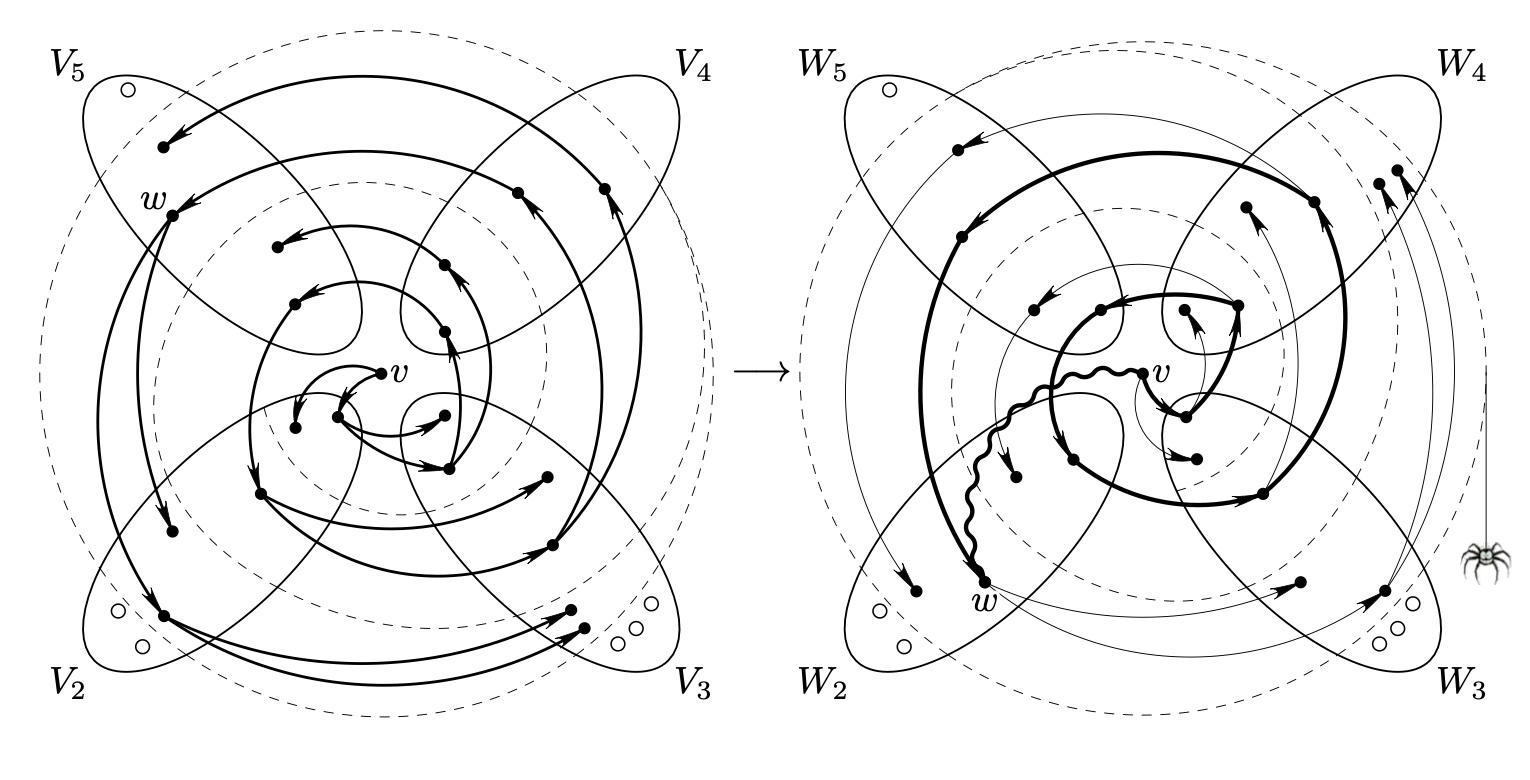
\includegraphics[width= 1\linewidth]{C7_SL2015IMO}
		\caption{\small\textit{\color{hoccungpi}Hình $3.$ Quy trình xây dựng chu trình.}}
		\vspace*{-10pt}
	\end{figure}
	Chú ý rằng, với cách đánh dấu các đỉnh, sau khi quy kết thúc; các đỉnh đã đánh dấu ở $V_i$ sẽ không có đỉnh kề trong $V_{i+1}$ mà đỉnh kề này lại chưa được đánh dấu. Hơn nữa, $v$ sẽ liên thông với tất cả các đỉnh được đánh dấu bởi một đường đi có hướng (đi theo chiều các mũi tên). 
	\vskip 0.1cm
	Bây giờ, ta chuyển mỗi đỉnh được đánh dấu thuộc tập $V_i$ sang tập $V_{i+1}$ (các đỉnh từ $V_i$ sang $V_{i+1}$ bây giờ sẽ được tô lại màu $i+1$ thay vì $i$). Theo nhận xét ở trên, ta thu được một cách tô màu mới vẫn thỏa mãn $2$ đỉnh kề nhau không cùng màu. Ký hiệu cách tô này là 
	\begin{align*}
		V_1 \cup W_2 \cup \dots \cup W_k.
	\end{align*}
	Quan sát rằng $v$ kề với một đỉnh $w \in W_2$ nào đó vì nếu không 
	\begin{align*}
		(V_1 \setminus \{v\}) \cup (W_2 \cup \{v\} ) \cup W_3 \cup \dots \cup W_k
	\end{align*}	
	sẽ là một cách tô màu mới mà rõ ràng  $|V_1 \setminus \{v\}| < |V_1|$, mâu thuẫn với cách chọn để ($1$) là một cách tô màu theo thứ tự. Nếu $w$ không được đánh dấu thì nghĩa là ban đầu $w \in V_2$. Nhưng khi đó ở bước đầu tiên của quy trình, đỉnh $w$ phải được đánh dấu và như vậy nó sẽ phải được chuyển sang $V_3$, nhưng điều này không xảy ra. Vì vậy $w$ là một đỉnh được đánh dấu và như vậy nó được chuyển từ $V_k$ sang $V_2$, nghĩa là ban đầu $w \in V_k$. 
	\vskip 0.1cm
	Cũng do $w$ được đánh dấu, tồn tại một đường đi có hướng từ $v$ đến $w$, ta thấy đường đi này đi xoay vòng qua tất cả các đỉnh thuộc $V_2,\dots,V_k$, vì thế có số cạnh chia hết cho $k-1$, vì nói riêng là một số chẵn. Chỉ cần nối thêm cạnh từ $w$ đến $v$; ta có ngay một chu trình có một số lẻ cạnh. Vậy ta đã xây dựng được một chu trình lẻ cạnh và có đủ $k$ màu và Bổ đề $2$ được chứng minh.
	\vskip 0.1cm
	Quay trở lại việc chứng minh Bổ đề $1$. Ta chọn một cách tô có thứ tự của $G$ như ($1$). Tương tự như trong Bổ đề $2$, ta đánh số các màu từ $1$ đến $k$. Với mọi tập con $C \subset \{1;2;\dots;k\}$ sao cho $|C|$ là số lẻ lớn hơn $1$, ta sẽ chỉ ra một chu trình đi qua một số lẻ đỉnh và có đủ tất cả các màu trong $C$. Tính chất này sẽ đảm bảo rằng: hai tập $C$ khác nhau cho hai chu trình khác nhau. Điều đó kéo theo Bổ đề $1$ được chứng minh, vì có đúng $2^{k-1} -k$ tập $C$ có lực lượng là số lẻ lớn hơn $1$. 
	\vskip 0.1cm
	Ký hiệu $V_C = \bigcup\limits_{c \in C} V_c$ và $G_C$ là đồ thị con của $G$ \textit{cảm sinh} từ $V_C$, nghĩa là đồ thị có có tập đỉnh là $V_C$ và hai đỉnh bất kỳ của $V_C$ kề nhau trong $G_C$ khi và chỉ khi chúng kề nhau trong $G$. Rõ ràng, cách tô màu $G$ bằng $k$ màu cảm sinh một cách tô màu $G_C$ bằng $|C|$ màu. Hơn nữa, cách tô màu này cũng là một cách tô màu tối ưu và theo thứ tự của $G_C$, vì nếu có một cách tô màu $(W_c)_{c \in C}$ khác  dùng ít màu hơn, hoặc dùng đúng $|C|$ màu và là một cách tô màu theo thứ tự của $G_C$; thì kết hợp cách tô $(W_c)_{c \in C}$ và cách tô các $V_i$ mà $ i \notin C$, ta sẽ thu được một cách tô màu tốt hơn, hoặc là một cách tô có thứ tự khác với  cách tô ($1$), vô lý!
	\vskip 0.1cm
	Từ đó, áp dụng Bổ đề $2$ cho đồ thị $G_C$ và cách tô màu theo thứ tự tương ứng là $(V_c)_{c \in C}$, ta thu được một chu trình lẻ và có đủ các màu trong $C$. Vậy Bổ đề $1$ được chứng minh và do đó bài toán được giải quyết.  
	\vskip 0.1cm
	Nói chung, những lời giải sử dụng mô hình đồ thị, đặc biệt là với những bài toán mà mô hình đồ thị được ẩn đi luôn đem lại hứng thú và sự phấn khích lớn. Đào sâu thêm, ta thấy rằng, dù mô hình đồ thị có thể giúp ta diễn đạt và hình dung bài toán trực quan hơn, nhưng trong một số trường hợp, điều đó là chưa đủ. Đôi khi, sau khi có được một mô hình đồ thị, ta còn cần phải phát hiện thêm các tính chất đặc biệt của đồ thị này. Tiếp theo, chúng ta cùng tìm hiểu hai loại đồ thị với cấu trúc đặc biệt. 
	\vskip 0.1cm
	$\pmb{3.}$ \textbf{\color{hoccungpi}Đồ thị lưỡng phân}	
	\vskip 0.1cm
	Khi gặp một đồ thị có rất nhiều cạnh và đỉnh, để nhìn thấy cấu trúc của đồ thị, thường ta sẽ phân hoạch tập đỉnh thành các tập con, sao cho mỗi cạnh của đồ thị có hai đầu thuộc hai tập con khác nhau. Một đồ thị mà tập đỉnh có thể được phân hoạch thành hai tập con có tính chất  như vậy được gọi là một đồ thị lưỡng phân, hay còn gọi là đồ thị hai phần.
	\vskip 0.1cm
	\textbf{\color{hoccungpi}Định nghĩa} $\pmb{3.1}$ (Đồ thị lưỡng phân)\textbf{\color{hoccungpi}.}
		Đồ thị $\pazocal{G}=(V,E)$ gọi là \textit{lưỡng phân} (hay \textit{hai phần}) nếu tập đỉnh $V$ có thể phân hoạch thành hai tập hợp $V_1, V_2$, sao cho mỗi cạnh của đồ thị $\pazocal{G}$ đều có một đầu mút thuộc $V_1$ và đầu mút còn lại thuộc $V_2$. 
	\begin{figure}[H]
		\vspace*{-5pt}
		\centering
		\captionsetup{labelformat= empty, justification=centering}
		\definecolor{cqcqcq}{rgb}{0.7529411764705882,0.7529411764705882,0.7529411764705882}
		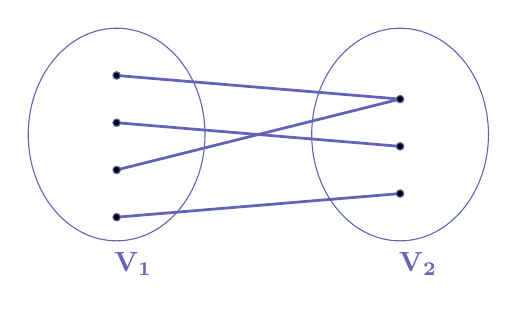
\begin{tikzpicture}[scale=0.3, hoccungpi]
			\draw [rotate around={90.:(5.,9.5)}] (5.,9.5) ellipse (4.5cm and 3.7416573867739413cm);
			\draw [rotate around={90.:(17.,9.5)}] (17.,9.5) ellipse (4.5cm and 3.7416573867739413cm);
			\draw [line width=1.pt] (5.,12.)-- (17.,11.);
			\draw [line width=1.pt] (5.,8.)-- (17.,11.);
			\draw [line width=1.pt] (5.,10.)-- (17.,9.);
			\draw [line width=1.pt] (5.,6.)-- (17.,7.);
			\draw (4.48,4.92) node[anchor=north west] {$\mathbf{V_1}$};
			\draw (16.54,4.94) node[anchor=north west] {$\mathbf{V_2}$};
			\begin{scriptsize}
				\draw [fill=black] (5.,12.) circle (4.5pt);
				\draw [fill=black] (5.,10.) circle (4.5pt);
				\draw [fill=black] (5.,8.) circle (4.5pt);
				\draw [fill=black] (5.,6.) circle (4.5pt);
				\draw [fill=black] (17.,11.) circle (4.5pt);
				\draw [fill=black] (17.,9.) circle (4.5pt);
				\draw [fill=black] (17.,7.) circle (4.5pt);
			\end{scriptsize}
		\end{tikzpicture}
		\caption{\small\textit{\color{hoccungpi} Hình $4.$ Minh họa đồ thị lưỡng phân.}}
		\vspace*{-10pt}
	\end{figure}
	Đồ thị lưỡng phân có những tính chất tương đối dễ thấy. Ví dụ, nếu tập đỉnh  $V$ được phân hoạch thành hai tập hợp $V_1, V_2$, thì $
	\sum\limits_{v \in V_1} \text{deg} (v) =  \sum\limits_{v \in V_2} \text{deg} (v) = |E|.$ Ngoài ra, số cạnh của đồ thị lưỡng phân $\pazocal{G}$ không vượt quá $|V_1| |V_2|$. Khi dấu bằng xảy ra, ta còn gọi đồ thị $\pazocal{G}$ là một đồ thị lưỡng phân đầy đủ và ký hiệu là $K_{a,b}$, với $a,b$ lần lượt là số phần tử của $V_1$, $V_2$.
	Tiếp theo, ta có một định lý để kiểm tra một đồ thị có là đồ thị lưỡng phân hay không. 
	\vskip 0.1cm
	\textbf{\color{hoccungpi}Định lý} $\pmb{3.1}$ (Dấu hiệu nhận biết)\textbf{\color{hoccungpi}.} 
		Cho  $\pazocal{G} = (V,E)$ là một đồ thị liên thông. Khi đó, các phát biểu sau là tương đương:
		\vskip 0.1cm
		$1.$ Đồ thị $\pazocal{G}$ lưỡng phân.
		\vskip 0.1cm
		$2.$ Các đỉnh của đồ thị $\pazocal{G}$ có thể tô bằng hai màu, sao cho hai đỉnh kề nhau không cùng màu.
		\vskip 0.1cm
		$3.$ Đồ thị $\pazocal{G}$ không chứa chu trình có số cạnh là lẻ.
		\vskip 0.1cm
	\textit{Chứng minh.} Ta dễ thấy rằng phát biểu $(1)$ tương đương với phát biểu $(2)$ vì $\pazocal{G}$ lưỡng phân tương đương với việc tập đỉnh của nó được phân hoạch thành hai tập $A,B$ mà mọi cạnh của $\pazocal{G}$ đều có một đầu mút thuộc $A$, một đầu thuộc $B$; và ta có thể tô các đỉnh thuộc $A$ bằng màu đen và các đỉnh thuộc $B$ màu trắng.
	\vskip 0.1cm
	Tiếp theo, ta chứng minh từ $(2)$ suy ra $(3)$. Nếu các đỉnh của $\pazocal{G}$ có thể được tô bằng hai màu sao cho hai đỉnh kề nhau bất kỳ khác màu mà có một chu trình lẻ cạnh thì dọc theo chu trình này, các đỉnh có màu đan xen nhau, vì thế đỉnh đầu và đỉnh cuối cùng màu, vô lý!
	\vskip 0.1cm
	Đảo lại, nếu $\pazocal{G}$ không chứa chu trình có số lẻ cạnh, ta có thể tô màu các đỉnh của nó như sau. Chọn một đỉnh gốc $u$ và tô đen, với mỗi đỉnh $v$, lấy tùy ý một đường đi từ $u$ đến $v$ (đường đi này luôn tồn tại vì $\pazocal{G}$ liên thông). Nếu đường đi này độ dài chẵn thì tô $v$ màu đen, nếu lẻ thì tô $v$ màu trắng. Cách tô này không phụ thuộc vào việc lựa chọn đường đi nào, vì mọi đường đi từ $u$ đến $v$ phải cùng tính chẵn lẻ, nếu không  bằng cách ghép một đường đi độ dài chẵn với một đường đi độ dài lẻ, ta thu được một chu trình độ dài lẻ. Hơn nữa, có thể thấy ngay cách tô này đảm bảo hai đỉnh kề nhau không cùng màu. 
	\vskip 0.1cm
	\textit{Lưu ý.} Giả thiết đồ thị $\pazocal{G}$ liên thông chỉ giúp ta dễ dàng hơn trong việc trình bày chứng minh trên. Kết quả của định lý trên vẫn đúng nếu ta bỏ đi giả thiết $\pazocal{G}$ liên thông. Tiếp theo, ta cùng xét một số ví dụ minh họa. 
	\vskip 0.1cm
	\textbf{\color{hoccungpi}Ví dụ} $\pmb{3.1}$ (Olympic Canada năm $2019$)\textbf{\color{hoccungpi}.} 
	Cho $n \geq 3$ điểm trên mặt phẳng sao cho không có ba điểm nào thẳng hàng. Hai người chơi một trò chơi như sau. Họ luân phiên chơi. Ở mỗi lượt chơi, người đến lượt chọn hai điểm chưa được nối và nối chúng lại với nhau. Người đầu tiên tạo ra một chu trình có số cạnh là lẻ thua cuộc. Tìm tất cả các giá trị của $n$ sao cho người chơi đầu tiên có chiến lược thắng cuộc.  
	\vskip 0.1cm
	\textbf{\color{hoccungpi}Nhận xét. } Mô hình đồ thị là rất rõ trong bài toán này. Do bài toán đề cập đến chu trình lẻ cạnh, nên ta nghĩ đến cấu trúc đồ thị lưỡng phân.  
	\vskip 0.1cm
	\textit{Lời giải.} Gọi hai người chơi là $A, B$ và giả sử $A$ là người chơi đầu tiên.
	\vskip 0.1cm
	Ở mọi thời điểm, khi người chơi vẫn có thể nối thêm một đường, thì đồ thị $\pazocal{G}$ vẫn chưa chứa chu trình lẻ cạnh. Do đó, nó vẫn là đồ thị lưỡng phân. Vì vậy, nếu người chơi $P$ thua, nghĩa là ở lượt chơi tiếp theo, với mọi cách nối hai điểm chưa được nối với nhau, anh ta đều tạo ra một đồ thị không còn là đồ thị lưỡng phân. Nói cách khác, đồ thị $\pazocal{G}$ ở thời điểm đó phải là đồ thị lưỡng phân đầy đủ $K_{a,b}$; với $a,b$ là các số nguyên không âm thỏa mãn $a+b =n$. Vì vậy, số cạnh của $\pazocal{G}$ khi đó là $ab$.
	\vskip 0.1cm
	Để $A$ giành chiến thắng, rõ ràng $ab$ phải là số lẻ. Nếu $n$ lẻ, thì chắc chắn một trong hai số $a,b$ chẵn. Suy ra $ab$ chẵn, và $A$ sẽ thua. 
	\vskip 0.1cm
	Nếu $n$ chẵn, chúng ta dự đoán trạng thái cuối cùng của đồ thị $\pazocal{G}$ sẽ là $K_{n/2,n/2}$ nếu cả $A$ và $B$ đều chơi một cách tối ưu. Vì vậy, nếu $n \equiv 0$ (mod $4$) thì $a=b = n/2$ đều chẵn và $A$ thua. Nếu $n \equiv 2$ (mod $4$) thì $a=b=n/2$ đều lẻ và $A$ thắng. Bây giờ, chúng ta sẽ chứng minh dự đoán trên.
	\vskip 0.1cm
	Chúng ta sẽ gọi một đồ thị lưỡng phân liên thông là {\it cân bằng} nếu các tập đỉnh đen và trắng  của nó (như trong Định lý $3.1$) của nó có lực lượng bằng nhau. (Điều kiện liên thông đảm bảo rằng cách tô màu là duy nhất, sai khác hoán vị các màu.) Tổng quát, một đồ thị hai phần được gọi là cân bằng nếu mỗi thành phần liên thông có nhiều hơn $1$ đỉnh của nó là cân bằng.
	\vskip 0.1cm
	Chiến lược chơi của người thắng cuộc là đảm bảo rằng sau mỗi lần anh ta chơi, đồ thị luôn là cân bằng và nói riêng số các đỉnh độc lập luôn là số chẵn.
	\vskip 0.1cm
	\textit{Trường hợp $1$: $n \equiv 2 \pmod 4$.} Người chơi $A$ có thể sử dụng chiến lược sau đây để đưa $\pazocal{G}$ về dạng $K_{n/2,n/2}$, và giành chiến thắng. Nhắc lại rằng, khi trò chơi chưa kết thúc, đồ thị là lưỡng phân. Hiển nhiên rằng ở nước đi đầu tiên $A$ sẽ nối $2$ đỉnh nào đó lại với nhau và do đó sau nước đi này thì đồ thị là cân bằng và số đỉnh cô lập là số chẵn. Ở mỗi lượt chơi sau đó của mình, tùy theo cách chơi của $B$ mà $A$ sẽ có cách chơi tương ứng:
	\vskip 0.1cm
	$\bullet$ Nếu $B$ nối một đỉnh cô lập với một đỉnh $S$ nào đó thuộc một thành phần liên thông không tầm thường (của đồ thị cân bằng đang có sau nước đi của $A$) thì $A$ sẽ nối một đỉnh cô lập khác với một đỉnh $T$ thuộc thành phần liên thông đó sao cho $S$ và $T$ có màu khác nhau.
	\vskip 0.1cm
	$\bullet$ Nếu $B$ nối $2$ đỉnh cô lập với nhau, hoặc nối $2$ đỉnh khác màu của một thành phần liên thông, hoặc nối $1$ đỉnh của một thành phần liên thông với $1$ đỉnh của một thành phần liên thông khác thì sau nước đi của $B$, đồ thị vẫn là cân bằng (và có số đỉnh cô lập là số chẵn). Khi này, $A$ chỉ cần nối $2$ đỉnh cô lập (nếu có) hoặc $2$ đỉnh không cô lập bất kỳ miễn là chúng không cùng màu.
	\vskip 0.1cm
	Ta dễ dàng kiểm tra được rằng cách chơi của $A$ đảm bảo rằng đồ thị luôn là cân bằng và đồ thị cuối cùng mà anh ta nhận được là $K_{n/2, n/2}$. 
	\vskip 0.1cm
	\textit{Trường hợp $2$: $n\equiv 0\pmod 4$.} Người chơi $B$ có thể sử dụng chiến lược giống hệt người chơi $A$ để đưa $\pazocal{G}$ về dạng  $K_{n/2,n/2}$, và giành chiến thắng.      
	\vskip 0.1cm
	Vậy người chơi $A$ có chiến lược  thắng khi và chỉ khi $n$ chia $4$ dư $2$.  
	\vskip 0.1cm
	\textbf{\color{hoccungpi}Ví dụ $\pmb{3.2}$} (Olympic Trung Quốc năm $2021$)\textbf{\color{hoccungpi}.}
	Một hội nghị có $n>3$ nhà khoa học, một số họ là bạn của nhau (quan hệ bạn bè là hai chiều và không có ai là bạn của chính bản thân mình). Người ta nhận thấy rằng, với mọi cách phân hoạch các nhà khoa học thành hai tập hợp khác rỗng, luôn tồn tại  hai người cùng thuộc một tập là bạn của nhau và hai người không cùng thuộc một tập là bạn của nhau.
	\vskip 0.1cm
	Trong ngày đầu tiên, mỗi nhà khoa học đưa ra một số nguyên không âm. Ở ngày thứ $k$, mỗi nhà khoa học thay đổi con số của mình bằng phần nguyên của trung bình cộng của các số của tất cả các bạn của mình trong ngày $k-1$. Chứng minh rằng, sau một số hữu hạn ngày, tất cả các nhà khoa học sẽ cùng đưa ra một con số.    
	\vskip 0.1cm
	\textit{Lời giải.}
	Chúng ta sẽ sử dụng mô hình đồ thị $\pazocal{G} = (V,E)$, trong đó mỗi nhà khoa học là một đỉnh và hai đỉnh nối với nhau nếu hai nhà khoa học này là bạn của nhau. Ta có $7$ nhận xét nhỏ như sau:
	\vskip 0.1cm
	$1.$ Đồ thị $\pazocal{G}$ liên thông. Thật vậy, giả sử $\pazocal{G}$ có ít nhất hai thành phần liên thông; gọi $S$ là một trong các thành phần liên thông. Xét phân hoạch $(V, V \setminus S)$: phân hoạch này không chứa hai người khác tập nhưng là bạn của nhau, mâu thuẫn.
	\vskip 0.1cm
	$2.$ Đồ thị $\pazocal{G}$ không là đồ thị lưỡng phân, vì nếu nó là đồ thị lưỡng phân thì ta phân hoạch tập đỉnh thành hai phía tương ứng. Khi đó, sẽ không tồn tại hai người là bạn của nhau cùng thuộc một tập. Điều này kéo theo đồ thị $\pazocal{G}$ phải chứa chu trình có số lẻ cạnh. Gọi một chu trình như vậy là $(P)$. 
	\vskip 0.1cm
	$3.$  Nhận xét trên kéo theo, giữa hai đỉnh bất kỳ $u,v$, tồn tại một đường đi từ $u$ đến $v$ có một số chẵn cạnh. Thật vậy, lấy một đỉnh $w$ thuộc chu trình $(P)$. Xét một đường đi có dạng $u-w-v$. Nếu đường đi này có một số chẵn cạnh thì ta có điều phải chứng minh; nếu nó có một số lẻ cạnh thì ta xét đường đi $u-w(P)w-v$, nghĩa là đường đi như trên, bổ sung thêm đường đi quanh $w$ bằng chu trình $(P)$: vì $(P)$ có một số lẻ cạnh nên nên đường đi này có một số chẵn cạnh. 
	\vskip 0.1cm
	$4.$ Xét dãy $(a_n)$, trong đó $a_n$ là số lớn nhất ở ngày thứ $n$. Dãy này  không tăng. Thật vậy, giả sử các nhà khoa học ở ngày thứ $n$ có số lớn nhất là $a_n$. Khi đó ở ngày $n+1$, mỗi nhà khoa học có số mới là trung bình cộng của các bạn của mình nên nó nhỏ hơn hoặc bằng $a_n$.
	\vskip 0.1cm
	$5.$  Mặt khác, dãy số nguyên $(a_n)$ bị chặn dưới bởi $0$, nên nó có giới hạn bằng $M$. Điều này có nghĩa là kể từ ngày thứ $N$ đủ lớn nào đó, ta luôn có $a_n = M$ với mọi $n \geq N$. 
	\vskip 0.1cm
	$6.$  \textit{Kể từ ngày thứ $N$, tất cả các nhà khoa học đều có số là $M$.} Để chỉ ra điều đó, ta sử dụng phương pháp phản chứng. Giả sử tồn tại nhà khoa học $v$ có số nhỏ hơn $M$ ở ngày thứ $k>N$, khi đó ở ngày thứ $k+1$, số của tất cả các bạn của $v$ sẽ nhỏ hơn $M$. Gọi khoảng cách giữa $2$ đỉnh (của một đồ thị liên thông) là số cạnh của đường đi ngắn nhất (sử dụng ít cạnh nhất) giữa chúng, ta sẽ có một dãy các sự kiện ở các ngày tiếp theo như sau:
	\vskip 0.1cm
	$\bullet$ Ở ngày $k+1$, tất cả các đỉnh có khoảng cách bằng $1$ đến $v$ đều có  số nhỏ hơn $M$.
	\vskip 0.1cm
	$\bullet$ Ở ngày $k+2$, tất cả các đỉnh có khoảng cách bằng $0,2$ đến $v$ đều có  số nhỏ hơn $M$.
	\vskip 0.1cm
	$\bullet$ Ở ngày $k+3$, tất cả các đỉnh có khoảng cách bằng $1,3$ đến $v$ đều có số nhỏ hơn $M$.
	\vskip 0.1cm
	\dots
	\vskip 0.1cm Ở ngày $k+2l$, tất cả các đỉnh có khoảng cách bằng $0,2,\dots,2l$ đến $v$ đều có số nhỏ hơn $M$.
	\vskip 0.1cm  
	$7.$ Tuy nhiên, vì giữa hai đỉnh $u,v$ bất kỳ đều tồn tại một đường đi có số chẵn cạnh, nên với $l$ đủ lớn, ở ngày $k+2l$, tất cả các nhà khoa học đều có số nhỏ hơn $M$, mâu thuẫn!!!  
	\vskip 0.1cm 
	Như vậy, ta có điều cần chứng minh.
	\vskip 0.1cm
	Trong các đồ thị lưỡng phân, có một loại đồ thị đặc biệt. Ỏ phần tiếp theo, ta sẽ cùng tìm hiểu loại đồ thị này. 
	\vskip 0.1cm
%	$\pmb{4.}$ \textbf{\color{hoccungpi}Đồ thị cây}
%	\vskip 0.1cm
%	Trong một số tình huống, ta có thể gặp những đồ thị mà số cạnh rất ít (còn gọi là đồ thị thưa). Khi đó, cấu trúc \textit{đồ thị cây} thường sẽ xuất hiện. Ta có định nghĩa về đồ thị cây như sau.
%	\vskip 0.1cm
%	\textbf{\color{hoccungpi}Định nghĩa} $\pmb{4.1}$ (Cây)\textbf{\color{hoccungpi}.}
%	Một đồ thị được gọi là một \textit{cây} nếu nó liên thông và không chứa một chu trình nào. 
%	\begin{figure}[H]
%		\vspace*{-5pt}
%		\centering
%		\captionsetup{labelformat= empty, justification=centering}
%		\definecolor{qqqqff}{rgb}{0.,0.,1.}
%		\begin{tikzpicture}[scale=0.4, hoccungpi]
%			\clip(3.52,0.5) rectangle (17.14,10.78);
%			\draw [line width=1.2pt] (9.,1.)-- (9.,4.);
%			\draw [line width=1.2pt] (9.,4.)-- (6.,7.);
%			\draw [line width=1.2pt] (6.,7.)-- (4.,10.);
%			\draw [line width=1.2pt] (6.,7.)-- (8.,10.);
%			\draw [line width=1.2pt] (9.,4.)-- (12.,10.);
%			\draw [line width=1.2pt] (9.,4.)-- (15.,7.);
%			\draw [line width=1.2pt] (15.,7.)-- (13.,10.);
%			\draw [line width=1.2pt] (15.,7.)-- (16.,10.);
%			\begin{scriptsize}
%				\draw [fill=qqqqff] (9.,1.) circle (5pt);
%				\draw [fill=qqqqff] (9.,4.) circle (5pt);
%				\draw [fill=qqqqff] (6.,7.) circle (5pt);
%				\draw [fill=qqqqff] (4.,10.) circle (5pt);
%				\draw [fill=qqqqff] (8.,10.) circle (5pt);
%				\draw [fill=qqqqff] (12.,10.) circle (5pt);
%				\draw [fill=qqqqff] (9.,4.) circle (5pt);
%				\draw [fill=qqqqff] (15.,7.) circle (5pt);
%				\draw [fill=qqqqff] (13.,10.) circle (5pt);
%				\draw [fill=qqqqff] (16.,10.) circle (5pt);
%			\end{scriptsize}
%		\end{tikzpicture}
%		\caption{\small\textit{\color{hoccungpi} Hình $5.$ Minh họa đồ thị cây.}}
%		\vspace*{-10pt}
%	\end{figure}
%	Lưu ý rằng, một đồ thị cây không chứa chu trình, do đó nó không thể chứa một chu trình lẻ cạnh, hay một đồ thị cây cũng đồng thời là một đồ thị lưỡng phân. Nếu đồ thị $\pazocal{G}$ gồm một số thành phần liên thông, mà mỗi thành phần liên thông là một cây, thì $\pazocal{G}$ còn được gọi là một \textit{rừng}. Ta có định lý sau:
%	\vskip 0.1cm 
%	\textbf{\color{hoccungpi}Định lý} $\pmb{4.1}$ (Các đặc trưng tương đương của cây)\textbf{\color{hoccungpi}.}
%	Cho  $\pazocal{G}$ là một đồ thị có $n$ đỉnh. Khi đó, các phát biểu sau là tương đương:
%	\vskip 0.1cm
%	$1.$ $\pazocal{G}$ là một cây;
%	\vskip 0.1cm
%	$2.$ $\pazocal{G}$ không có chu trình và có $n-1$ cạnh;
%	\vskip 0.1cm
%	$3.$ $\pazocal{G}$ liên thông và có $n-1$ cạnh;
%	\vskip 0.1cm
%	$4.$ $\pazocal{G}$ không có chu trình và nếu bổ sung vào một cạnh nối hai đỉnh không kề nhau thì xuất hiện một chu trình duy nhất;
%	\vskip 0.1cm
%	$5.$ $\pazocal{G}$ liên thông và nếu bỏ đi một cạnh bất kỳ thì $\pazocal{G}$ mất tính liên thông;
%	\vskip 0.1cm
%	$6.$ Mỗi cặp đỉnh trong $\pazocal{G}$ được nối với nhau bằng một đường đi duy nhất.
%	\vskip 0.1cm
%	Việc chứng minh định lý trên không khó. Bạn đọc quan tâm có thể tìm hiểu chi tiết chứng minh trong [$4$]. Để minh họa, chúng ta hãy cùng xét hai ví dụ sau.
%	\vskip 0.1cm
%	\textbf{\color{hoccungpi}Ví dụ} $\pmb{4.1}$ (Bài toán dự tuyển thi IMO  năm $2019$, Croatia đề xuất)\textbf{\color{hoccungpi}.}
%	Trong một mạng xã hội, có $2019$ người dùng, một số họ là bạn của nhau (quan hệ bạn bè là quan hệ $2$ chiều). Ban đầu, có $1010$ người mà mỗi người có đúng $1009$ bạn và có $1009$ người mà mỗi người có đúng $1010$ bạn. Tuy nhiên, quan hệ bạn bè trong mạng này không bền vững, những sự kiện tương tự như sự kiện sau có thể lần lượt xảy ra (mỗi thời điểm chỉ có đúng một sự kiện xảy ra):
%	\vskip 0.1cm
%	Ký hiệu $A,B,C$ là ba người dùng sao cho $A$ là bạn của cả $B$ và $C$, nhưng $B$ và $C$ không phải là bạn của nhau. Khi đó $B$ và $C$ sẽ trở thành bạn, đồng thời $A$ không còn là bạn của cả $B$ và $C$.
%	\vskip 0.1cm
%	Chứng minh rằng, với mọi cấu hình ban đầu, tồn tại một dãy các sự kiện như sự kiện trên mà sau đó, mỗi người dùng chỉ còn tối đa một người bạn.  
%	\vskip 0.1cm
%	\textbf{\color{hoccungpi}Nhận xét. } Bài toán trên rõ ràng có thể phát biểu lại bằng ngôn ngữ của lý thuyết đồ thị như sau. Cho một đồ thị $\pazocal{G}$ có $2019$ đỉnh. Trong đó, $1010$ đỉnh có bậc $1009$ và $1009$ đỉnh có bậc $1010$. Ở mỗi bước, ta có thể: \textit{``Chọn ra ba đỉnh $A,B,C$ mà $A$ nối với cả $B$ và $C$; còn $B,C$ không nối với nhau. Sau đó, xóa hai cạnh $AB,AC$ và thêm cạnh $BC$ vào đồ thị $\pazocal{G}$.''}
%	\vskip 0.1cm
%	Gọi mỗi thao tác trên là một thao tác \textit{đảo cạnh}. Ta cần chứng minh rằng, thông qua một dãy các thao tác đảo cạnh, ta có thể tạo ra một đồ thị mà mỗi đỉnh của đồ thị có bậc không vượt quá $1$. Không khó để nhận ra, đây chính là một đồ thị rừng. 
%	\vskip 0.1cm
%	\textit{Lời giải.}
%	Chú ý rằng một thao tác đảo cạnh bảo toàn tính chất: đồ thị $\pazocal{G}$ có ít nhất một đỉnh bậc lẻ và không phải là một đồ thị đầy đủ (tính chất này là hiển nhiên). Ta cũng chú ý rằng, đồ thị ban đầu là liên thông (chứng minh được dành cho bạn đọc như một bài tập). Bây giờ, ta mô tả một thuật toán gồm hai bước để chuyển đồ thị ban đầu về một đồ thị mà bậc của mỗi đỉnh không vượt quá $1$. 
%	\vskip 0.1cm
%	\textit{Bước $1$: Tồn tại một dãy các thao tác đảo cạnh để chuyển đồ thị ban đầu về một đồ thị dạng cây.}
%	\vskip 0.1cm
%	\textit{Chứng minh.} Vì số cạnh của đồ thị giảm đi $1$ sau mỗi thao tác đảo cạnh, ta chỉ cần chứng minh: chừng nào đồ thị $\pazocal{G}$ còn chứa một chu trình, thì tồn tại một thao tác đảo cạnh sao cho đồ thị mới được tạo ra vẫn liên thông. Ta đi chứng minh đồ thị chứa một chu trình $\pazocal{Z}$ và các đỉnh $A,B,C$ sao cho hai đỉnh $A$ và $B$ kề nhau trong chu trình $\pazocal{Z}$, đỉnh $C$ không nằm trong chu trình $\pazocal{Z}$ và kề với đỉnh $A$ nhưng không kề với đỉnh $B$. Bỏ hai cạnh $AB, AC$ và thêm cạnh $BC$ sẽ bảo toàn tính liên thông của đồ thị và khẳng định được chứng minh.  
%	\begin{figure}[H]
%		\vspace*{-5pt}
%		\centering
%		\captionsetup{labelformat= empty, justification=centering}
%		\definecolor{qqqqff}{rgb}{0.,0.,1.}
%		\begin{tikzpicture}[scale=0.25,hoccungpi]
%			\draw (18.,30.)-- (12.,24.);
%			\draw (12.,24.)-- (18.,18.);
%			\draw (18.,18.)-- (26.,18.);
%			\draw (26.,18.)-- (32.,24.);
%			\draw (32.,24.)-- (26.,30.);
%			\draw (26.,30.)-- (18.,30.);
%			\draw (32.,24.)-- (38.,30.);
%			\draw [dash pattern=on 2pt off 2pt] (26.,30.)-- (38.,30.);
%			\draw (32.1,24.2) node[anchor=north west] {$A$};
%			\draw (25.5,32) node[anchor=north west] {$B$};
%			\draw (37.6,32) node[anchor=north west] {$C$};
%			\begin{scriptsize}
%				\draw [fill=qqqqff] (18.,30.) circle (5pt);
%				\draw [fill=qqqqff] (12.,24.) circle (5pt);
%				\draw [fill=qqqqff] (18.,18.) circle (5pt);
%				\draw [fill=qqqqff] (26.,18.) circle (5pt);
%				\draw [fill=qqqqff] (32.,24.) circle (5pt);
%				\draw [fill=qqqqff] (26.,30.) circle (5pt);
%				\draw [fill=qqqqff] (38.,30.) circle (5pt);
%			\end{scriptsize}
%		\end{tikzpicture}
%		\caption{\small\textit{\color{hoccungpi}Hình $6.$ Nếu đồ thị $\pazocal{G}$ chứa chu trình $\pazocal{Z}$, thì ta vẫn có thể giảm số cạnh của nó.}}
%		\vspace*{-10pt}
%	\end{figure}
%	Để tìm chu trình $\pazocal{Z}$ và các đỉnh $A,B,C$; ta sử dụng hai chiến lược sau. Nếu đồ thị $\pazocal{G}$ chứa một tam giác, ta xét một đồ thị con đầy đủ lớn nhất $K$. Rõ ràng $K$ chứa ít nhất ba đỉnh. Vì đồ thị $\pazocal{G}$ không là đồ thị đầy đủ, tồn tại một đỉnh $C$ không thuộc $K$ và kề với một đỉnh $A$ thuộc $K$. Do tính lớn nhất của $K$, có một đỉnh $B$ thuộc $K$ không kề với đỉnh $C$, và do đó ta có thể chọn chu trình $\pazocal{Z}$ trong $K$ và đi qua cạnh $AB$. 
%	\vskip 0.1cm
%	Nếu đồ thị $\pazocal{G}$ không chứa tam giác, ta xét một chu trình ngắn nhất $\pazocal{Z}$ trong đồ thị $\pazocal{G}$. Chu trình này không thể là một chu trình Hamilton (tức là chu trình đi qua tất cả các đỉnh của đồ thị, mỗi đỉnh đúng một lần). Thật vậy, nếu không, do tính nhỏ nhất của $\pazocal{Z}$, đồ thị $\pazocal{G}$ sẽ không chứa thêm một cạnh nào nữa, dẫn đến mỗi đỉnh của đồ thị $\pazocal{G}$ đều có bậc bằng $2$, mâu thuẫn với việc đồ thị luôn có đỉnh bậc lẻ. Như vậy, $\pazocal{Z}$ không là một chu trình Hamilton và vì thế có thể tìm được một đỉnh $C$ không thuộc $\pazocal{Z}$ và kề với một đỉnh $A$ thuộc $\pazocal{Z}$. Do đồ thị $\pazocal{G}$ không chứa tam giác, đỉnh $C$ sẽ không kề với bất kỳ đỉnh $B$ nào kề với $A$ trong $\pazocal{Z}$ và ta chọn được chu trình $\pazocal{Z}$ và ba đỉnh $A,B,C$.    
%	\begin{figure}[H]
%		\vspace*{-5pt}
%		\centering
%		\captionsetup{labelformat= empty, justification=centering}
%		\definecolor{qqqqff}{rgb}{0.,0.,1.}
%		\definecolor{cqcqcq}{rgb}{0.7529411764705882,0.7529411764705882,0.7529411764705882}
%		\begin{tikzpicture}[scale=0.25, hoccungpi]
%			\draw (18.,30.)-- (12.,24.);
%			\draw (12.,24.)-- (18.,18.);
%			\draw (18.,18.)-- (26.,18.);
%			\draw (26.,18.)-- (32.,24.);
%			\draw (32.,24.)-- (26.,30.);
%			\draw (26.,30.)-- (18.,30.);
%			\draw (32.,24.)-- (38.,30.);
%			\draw [dash pattern=on 2pt off 2pt] (26.,30.)-- (38.,30.);
%			\draw (32.1,24.2) node[anchor=north west] {$A$};
%			\draw (25.5,32) node[anchor=north west] {$B$};
%			\draw (37.6,32) node[anchor=north west] {$C$};
%			\draw (18.,30.)-- (26.,18.);
%			\draw (26.,30.)-- (18.,18.);
%			\draw (12.,24.)-- (32.,24.);
%			\draw (18.,30.)-- (18.,18.);
%			\draw (26.,30.)-- (26.,18.);
%			\draw (12.,24.)-- (26.,30.);
%			\draw (26.,18.)-- (12.,24.);
%			\draw (18.,30.)-- (32.,24.);
%			\draw (32.,24.)-- (18.,18.);
%			\begin{scriptsize}
%				\draw [fill=qqqqff] (18.,30.) circle (5pt);
%				\draw [fill=qqqqff] (12.,24.) circle (5pt);
%				\draw [fill=qqqqff] (18.,18.) circle (5pt);
%				\draw [fill=qqqqff] (26.,18.) circle (5pt);
%				\draw [fill=qqqqff] (32.,24.) circle (5pt);
%				\draw [fill=qqqqff] (26.,30.) circle (5pt);
%				\draw [fill=qqqqff] (38.,30.) circle (5pt);
%			\end{scriptsize}
%		\end{tikzpicture}
%		\caption{\small\textit{\color{hoccungpi} Hình $7.$ Minh họa cách tìm chu trình $\pazocal{Z}$ và ba điểm $A,B,C$.}}
%		\vspace*{-10pt}
%	\end{figure} 
%	\textit{Bước $2$: Mọi đồ thị dạng cây đều có thể chuyển về một đồ thị có bậc mỗi đỉnh không vượt quá $1$ thông qua một dãy các thao tác đảo cạnh.}
%	\vskip 0.1cm
%	\textit{Chứng minh.} Để ý rằng thao tác đảo cạnh  bảo toàn tính chất không chứa chu trình. Do đó, kể từ một cây, sau các thao tác đảo cạnh, ta luôn có một đồ thị không chứa chu trình. Ngoài ra, mỗi thao tác đảo cạnh sẽ giảm số cạnh của đồ thị đi $1$ nên  đến một lúc nào đó ta không thể thực hiện thêm một thao tác đảo cạnh nào nữa. Khi này bậc của mỗi đỉnh của đồ thị này không vượt quá $1$. Thật vậy, nếu có một đỉnh $A$ với  kề với hai đỉnh $B,C$ nào đó (khi đó $B,C$ không kề nhau vì đồ thị đang xét không chứa chu trình) thì ta có thể thực hiện thêm một thao tác đảo cạnh.
%	\vskip 0.1cm
%	\textbf{\color{hoccungpi}Ví dụ} $\pmb{4.2}$ (Kỳ thi chọn đội tuyển Mỹ tham dự Egmo $2020$)\textbf{\color{hoccungpi}.} Cho $\pazocal{G}=(V,E)$ là một  đồ thị đơn có $n$ đỉnh. Một cạnh $e$ của của nó được gọi là một \textit{cạnh cổ chai} nếu có thể phân hoạch $V$ thành hai  tập $A,B$ thỏa mãn:
%	\vskip 0.1cm
%	$1.$ Có tối đa $100$ cạnh của $\pazocal{G}$ có một đầu mút thuộc $A$ và đầu mút còn lại thuộc $B$;
%	\vskip 0.1cm
%	$2.$ Cạnh $e$ là một trong số các cạnh như vậy.
%	\vskip 0.1cm 
%	Chứng minh rằng đồ thị $\pazocal{G}$ có tối đa $100(n-1)$ cạnh cổ chai.
%	\vskip 0.1cm
%	\textbf{\color{hoccungpi}Nhận xét. } Con số $100(n-1)$ ít nhiều gợi ý cho ta $100$ cấu trúc cây trong đồ thị $\pazocal{G}$. 
%	\vskip 0.1cm
%	\textit{Lời giải.} Gọi $F_1$ là một rừng lớn nhất trong $\pazocal{G}$ (nếu $\pazocal{G}$ liên thông thì $F_1$ chính là một cây). Xóa đi các cạnh của $F_1$ và gọi $F_2$ là rừng lớn nhất trong đồ thị mới nhận được (vẫn có $n$ đỉnh). Cứ tiếp tục như vậy, cho đến $F_{100}$ là rừng lớn nhất trong đồ thị nhận được khi xóa đi các cạnh của  $F_1\cup F_2\cup \cdots \cup F_{99}$. Giả sử ngược lại, $\pazocal{G}$ có nhiều hơn $100(n-1)$ cạnh cổ chai. Mỗi rừng $F_i$ (với $i=1,\dots,100$) (có $n$ đỉnh) có tối đa $n-1$ cạnh. Do vậy, tổng số các cạnh trong $F_1\cup F_2\cup \cdots \cup F_{100}$ không vượt quá $100(n-1)$. Vì vậy, vẫn tồn tại một cạnh cổ chai không nằm trong bất kỳ $F_{i}, i=1, 2, \ldots, 100$ nào.
%	Gọi $x-y$ là một cạnh như vậy ($x,y$ là hai đỉnh của đồ thị). Rõ ràng, trong mỗi $F_i$, có một đường đi từ $x$ đến $y$ vì nếu không, thêm cạnh $x-y$ vào $F_i$ ta vẫn có một rừng (mâu thuẫn với cách chọn $F_i$ lớn nhất). Vì vậy, trong $\pazocal{G}$ có ít nhất $101$ đường đi từ $x$ đến $y$, hơn nữa hai đường đi bất kỳ đều không có cạnh chung. Tuy nhiên, khi đó cạnh $x-y$ không thể là cạnh cổ chai. Thật vậy, gọi $A,B$ là phân hoạch của $V$ tương ứng với cạnh cổ chai $x-y$. Với mỗi $i$, đường đi  trong $F_i$ từ $x$ đến $y$ phải chứa một cạnh nối một đỉnh thuộc $A$ và một đỉnh thuộc $B$. Tóm tại, ta tìm được $101$ cạnh của $G$ mà một đầu mút thuộc $A$ và  đầu mút còn lại thuộc $B$ (mâu thuẫn với điều kiện $(1)$). 
%	\vskip 0.1cm
%	Hy vọng rằng qua một số lý thuyết và bài tập minh họa, bạn đọc đã ít nhiều thấy được tiềm năng, sự phong phú và mối liên hệ của lý thuyết đồ thị với nhiều mảng kiến thức khác. Rõ ràng, khi mô hình hóa được một bài toán dưới dạng ngôn ngữ đồ thị, ta có thể tìm ra định hướng tốt trong việc tìm kiếm lời giải. Cụ thể hơn, khi gặp một mô hình đồ thị có nhiều cạnh, ta có thể liên tưởng đến cấu trúc đồ thị lưỡng phân; ngược lại, một mô hình đồ thị ít cạnh làm chúng ta liên tưởng đến đồ thị dạng cây, rừng.  
%	Phần cuối của bài viết này là một số bài tập giúp rèn luyện thêm kỹ năng phát hiện và sử dụng các cấu trúc đồ thị lưỡng phân và cây.   
%	\vskip 0.1cm
%	$\pmb{5.}$ \textbf{\color{hoccungpi}Một số bài toán tự rèn luyện}
%	\vskip 0.1cm
%	\textbf{\color{hoccungpi}Bài $\pmb{1.}$} \textit{(Olympic Canada năm $2020$)} Cho đồ thị $\pazocal{G}$ có $19998$ đỉnh. Mỗi đồ thị con gồm $9999$ đỉnh của $\pazocal{G}$ đều chứa ít nhất $9999$ cạnh. Hỏi $\pazocal{G}$ có ít nhất bao nhiêu cạnh?
%	\vskip 0.1cm
%	\textbf{\color{hoccungpi}Bài $\pmb{2.}$}\textit{(Mở rộng Bài $2$)}  Cho đồ thị $\pazocal{G}$ có $2n$ đỉnh. Mỗi đồ thị con $n$ đỉnh của  $\pazocal{G}$ đều có ít nhất $n$ cạnh. Chứng minh rằng $\pazocal{G}$ có ít nhất $5n$ cạnh.
%	\vskip 0.1cm
%	\textbf{\color{hoccungpi}Bài $\pmb{3.}$} \textit{(Olympic Liên bang Nga năm $2004$)} Một quốc gia có $1001$ thành phố.  Hai thành phố bất kỳ được nối với nhau bằng một con đường một chiều. Mỗi thành phố có $500$ con đường đi ra và $500$ con đường đi vào. Có một tổ chức ly khai xuất hiện và chiếm đóng $668$ thành phố. Chứng minh rằng, trong khu vực ly khai này, từ mỗi thành phố đều có có thể đi đến một thành phố khác.
%	\vskip 0.1cm
%	\textbf{\color{hoccungpi}Bài $\pmb{4.}$}  Cho đồ thị $\pazocal{G} = (V,E)$ thỏa mãn $|E| = |V| +4$. Chứng minh rằng, trong $\pazocal{G}$ có
%	hai chu trình không có cạnh chung. 
	\vskip 0.1cm
	\textbf{\color{hoccungpi}Tài liệu}
	\vskip 0.1cm
	[$1$] Đỗ Đức Thái, \textit{Chuyên đề học tập toán $11$}. NXB Đại học Sư phạm Hà Nội. 
	\vskip 0.1cm
	[$2$] Hà Huy Khoái, \textit{Chuyên đề học tập toán $11$}. NXB Giáo dục Việt Nam. 
	\vskip 0.1cm
	[$3$] Asratian, Armen S.; Denley, Tristan M. J.; Häggkvist, Roland, \textit{Bipartite Graphs and their Applications}. Cambridge University Press, $1998$.
	\vskip 0.1cm
	[$4$] Bender, Edward A.; Williamson, S. Gill , \textit{Lists, Decisions and Graphs  With an Introduction to Probability}, $2010$.
	\vskip 0.1cm
	[$5$] Titu Andreescu, Bogdan Enescu, \textit{Mathematical Olympiad Treasures}. Springer, $2011$.
	\vskip 0.1cm                 
	[$6$] Website \url{https://artofproblemsolving.com}. 
\end{multicols}
	\newpage
	
	\setcounter{figure}{0}
	\thispagestyle{thachthuctoanhocnone}
\pagestyle{thachthuctoanhoc}
\everymath{\color{thachthuctoanhoc}}
\graphicspath{{../thachthuctoanhoc/pic/}}
\begingroup
\AddToShipoutPicture*{\put(0,616){\includegraphics[width=19.3cm]{../thachthuctoanhoc/bannerthachthuc}}}
\centering
\vspace*{4cm}
\endgroup
\vspace*{-8pt}
\begin{tBox}
	\begin{itemize}[leftmargin = 13pt, itemsep = 1.0pt] 
		\item Mỗi bài toán đề xuất (kèm theo lời giải) cần được nêu rõ là bài sáng tác hay bài sưu tầm.
		%		\item Mỗi bài toán đề xuất (kèm theo lời giải) cần được nêu rõ là bài sáng tác hay bài sưu tầm (nếu là bài sưu tầm, cần ghi rõ nguồn).
		\item Bài giải cho mỗi bài toán cần được trình bày trong một file riêng hoặc
		một tờ giấy riêng.
		\item  Người đề xuất bài toán hoặc gửi bài giải cho các bài toán trong mục ``Thách thức kỳ này" cần ghi rõ họ, đệm, tên và nơi làm việc/học tập, số điện thoại liên hệ. Nếu là học sinh (hoặc sinh viên) cần ghi rõ là học sinh lớp mấy (hoặc sinh viên năm thứ mấy).
		\item Các bài toán trong mục Thách thức kỳ này hướng tới các độc giả là học sinh phổ thông; được phân chia thành các mức độ $B$, $A$, và được sắp xếp theo độ khó tăng dần, theo đánh giá chủ quan của Ban biên tập. Các bài toán mức độ $B$ không đòi hỏi các kiến thức vượt quá chương trình môn Toán cấp THCS; các bài toán mức độ $A$ không đòi hỏi các kiến thức vượt quá chương trình môn Toán cấp THPT.
		\item Cách thức gửi bài toán đề xuất hoặc lời giải: gửi file thu được bằng cách scan, ảnh chụp (rõ nét) của bản viết tay, hoặc được soạn thảo bằng các phần mềm Latex, Word tới \url{bbt@pi.edu.vn} hoặc gửi qua đường bưu điện tới Tòa soạn (xem địa chỉ tại bìa $2$).
		\item Hạn gửi lời giải cho các bài toán P$751$--P$760$: trước ngày $15/12/2023$.
	\end{itemize}
\end{tBox}
\begin{center}
	\vspace*{-5pt}
	\textbf{\color{thachthuctoanhoc}\color{thachthuctoanhoc}\color{thachthuctoanhoc}\color{thachthuctoanhoc}\color{thachthuctoanhoc}THÁCH THỨC KỲ NÀY}
	\vspace*{-5pt}
\end{center}
\begin{multicols}{2}
	\setlength{\abovedisplayskip}{4pt}
	\setlength{\belowdisplayskip}{4pt}
	{\color{thachthuctoanhoc}{\usefont{T5}{qag}{b}{n} P751.}}
	(Mức $B$) Người ta ghép khít năm hình chữ nhật bằng nhau với nhau, để được một hình dài $27$cm và rộng $15 $cm, như ở hình vẽ dưới đây. Biết rằng, đoạn thẳng $A C$ chia hình đó thành hai phần có diện tích bằng nhau. Hãy tính độ dài đoạn thẳng $A B$.
	\begin{figure}[H]
		\vspace*{-10pt}
		\centering
		\captionsetup{labelformat= empty, justification=centering}
		\definecolor{qqqqff}{rgb}{0,0,1}
		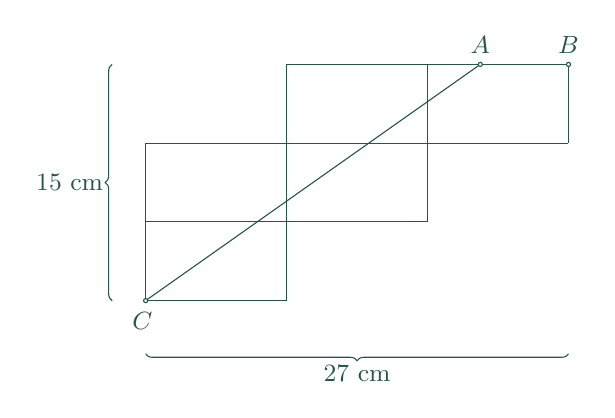
\begin{tikzpicture}[scale=0.5,thachthuctoanhoc, node font=\small]
			\draw  (-4,2)-- (-4,-2);
			\draw  (-4,-2)-- (-0.42,-2);
			\draw  (-0.42,-2)-- (-0.42,4);
			\draw  (-4,2)-- (6.74,2);
			\draw  (6.74,2)-- (6.74,4);
			\draw  (6.74,4)-- (-0.42,4);
			\draw  (3.16,4)-- (3.16,0);
			\draw  (3.16,0)-- (-4,0);
			\draw  (-4,-2)-- (4.5,4);
			\draw[decoration={brace,mirror,raise=5pt},decorate]
			(-4,-3) -- node[below = 6pt] {$27\text{ cm}$} (6.74,-3);
			\draw[decoration={brace,mirror,raise=5pt},decorate]
			(-4.5,4) -- node[left = 5pt] {$15\text{ cm}$} (-4.5,-2);
			\draw [fill=white] (-4,-2) circle (1.5pt);
			\draw (-4.08,-2.52) node {$C$};
			\draw [fill=white] (6.74,4) circle (1.5pt);
			\draw (6.74,4.5) node {$B$};
			\draw [fill=white] (4.5,4) circle (1.5pt);
			\draw (4.5,4.5) node {$A$};
		\end{tikzpicture}
		\vspace*{-10pt}
	\end{figure}
	\begin{flushright}
		\textit{Đăng Hải, Hà Nội (st)}
	\end{flushright}
	{\color{thachthuctoanhoc}{\usefont{T5}{qag}{b}{n} P752.}}
	(Mức $B$) Cho $x,y,z$ là các số thực thoả mãn $x^2y+y^2z+z^2x=1$ và $xy^2+yz^2+zx^2=2$. Tính giá trị biểu thức
	\begin{align*}
		P=\left(\!x^2\!+\!xy\!+\!y^2\!\right)\!\left(\!y^2\!+\!yz\!+\!z^2\!\right)\!\left(\!z^2\!+\!zx\!+\!x^2\!\right).
	\end{align*}
	\begin{flushright}
		\textit{Trần Quốc Luật, Tp. Hồ Chí Minh}
	\end{flushright}
	{\color{thachthuctoanhoc}{\usefont{T5}{qag}{b}{n} P753.}}
	(Mức $B$) Cho đường tròn $(O)$ với đường kính $AB = 2R$. Gọi $C$ là trung điểm của $OA$. $M$ là một điểm nằm trên $(O)$. Đường thẳng $MC$ cắt $(O)$ tại điểm thứ hai $D$.  Đường thẳng qua $D$ và vuông góc với $AB$, cắt $(O)$ tại điểm thứ hai $E$. Đường thẳng $ME$ cắt đường thẳng $AB$ tại điểm $F$. Tìm vị trí của điểm $M$  sao cho tổng $EF + MC$ có giá trị nhỏ nhất.
	\begin{figure}[H]
%		\vspace*{5pt}
		\centering
		\captionsetup{labelformat= empty, justification=centering}
		\definecolor{qqwuqq}{rgb}{0.,0.39215686274509803,0.}
		\definecolor{uuuuuu}{rgb}{0.26666666666666666,0.26666666666666666,0.26666666666666666}
		\definecolor{xdxdff}{rgb}{0.49019607843137253,0.49019607843137253,1.}
		\definecolor{ududff}{rgb}{0.30196078431372547,0.30196078431372547,1.}
		\begin{tikzpicture}[thachthuctoanhoc]
			\draw[color=qqwuqq,fill=qqwuqq,fill opacity=0.10000000149011612] (-1.5617418181909823,1.) -- (-1.5617418181909823,1.1880461622337974) -- (-1.7497879804247796,1.1880461622337974) -- (-1.7497879804247796,1.) -- cycle; 
			\draw  (0.,1.) circle (2.cm);
			\draw  (-2.,1.)-- (2.,1.);
			\draw  (-4.,1.)-- (0.4991521613769648,2.936710386142622);
			\draw  (0.4991521613769648,2.936710386142622)-- (-1.7497879804247796,0.03137105991975908);
			\draw  (-2.,1.)-- (-4.,1.);
			\draw  (-1.7497879804247796,1.968628940080241)-- (-1.7497879804247796,0.03137105991975908);
				\draw [fill=white] (0.,1.) circle (1.5pt);
				\draw (0.09082211690268885,1.2491318135923188) node {$O$};
				\draw [fill=white] (-2.,1.) circle (1.5pt);
				\draw (-2.2228335500515635,0.7335225357666101) node {$A$};
				\draw [fill=white] (2.,1.) circle (1.5pt);
				\draw (2.2449153240669926,0.9831943806090713) node {$B$};
				\draw [fill=white] (-1.,1.) circle (1.5pt);
				\draw (-1.0793025882235996,1.2757255568906436) node {$C$};
				\draw [fill=white] (0.4991521613769648,2.936710386142622) circle (1.5pt);
				\draw (0.6492907261675084,3.2170688176683497) node {$M$};
				\draw [fill=white] (-1.7497879804247796,0.03137105991975908) circle (1.5pt);
				\draw (-1.9435992454191537,-0.1869303245172173) node {$D$};
				\draw [fill=white] (-1.7497879804247796,1.968628940080241) circle (1.5pt);
				\draw (-1.917005502120829,2.233100315630334) node {$E$};
				\draw [fill=white] (-4.,1.) circle (1.5pt);
				\draw (-4.00461435103932,0.737413058716358) node {$F$};
		\end{tikzpicture}
		\vspace*{-10pt}
	\end{figure}
	\begin{flushright}
		\textit{Trần Thanh Hưng, Phú Yên}
	\end{flushright}
	{\color{thachthuctoanhoc}{\usefont{T5}{qag}{b}{n} P754.}}
	(Mức $B$) Cho $a, b, c$ là các số thực dương. Chứng minh rằng
	\begin{align*}
		&\frac{b+c}{\sqrt{\!a^2\!+\!b c}\!+\!\!\sqrt{\!a(b+c)}}\!+\!\frac{c\!+\!a}{\sqrt{\!b^2\!+\!c a}\!+\!\!\sqrt{\!b(c\!+\!a)}}\\
		&+\frac{a+b}{\sqrt{c^2+a b}+\sqrt{c(a+b)}} \geq \frac{3}{\sqrt{2}} .
	\end{align*}
	\begin{flushright}
		\textit{Nguyễn Việt Hùng, Hà Nội}
	\end{flushright}
	{\color{thachthuctoanhoc}{\usefont{T5}{qag}{b}{n} P755.}}
	(Mức $B$) Trong một hình chữ nhật có kích thước $5\times 10$, lấy $1351$ điểm đôi một phân biệt tuỳ ý. Chứng minh rằng, tồn tại một hình tròn bán kính bằng $\dfrac14$ chứa ít nhất $4$ điểm trong số các điểm đã lấy.
	\begin{flushright}
		\textit{Phạm Nhật Nguyệt, Hải Phòng (st)}
	\end{flushright}
	{\color{thachthuctoanhoc}{\usefont{T5}{qag}{b}{n} P756.}}
	(Mức $B$) Ta gọi số nguyên dương $n$ là ``số đẹp" nếu trong $22$ số: $5,n+5,2n+5,\ldots,21n+5$, tồn tại một số có cùng số dư với tích tất cả các số đó, trong phép chia cho $23$. Hãy tìm tất cả các số đẹp.
	\begin{flushright}
		\textit{Hà Duy Hưng, Hà Nội}
	\end{flushright}
	{\color{thachthuctoanhoc}{\usefont{T5}{qag}{b}{n} P757.}}
	(Mức $A$) Với mỗi số nguyên dương $n$, ta kí hiệu $a_n$ là nghiệm thực lớn nhất của phương trình
	\begin{align*}
		x^{2023}-nx^{2022}-nx^{2021}-\cdots-nx+1=0
	\end{align*}
	Xác định tất cả các số thực $C$, để 
	\begin{align*}
		a_1+\cdots+a_n>C. n^2
	\end{align*}
	với mọi số nguyên dương $n$.
	\begin{flushright}
		\textit{Tô Trung Hiếu, Nghệ An}
	\end{flushright}
	{\color{thachthuctoanhoc}{\usefont{T5}{qag}{b}{n} P758.}}
	(Mức $A$) Tìm số thực $k$ lớn nhất sao cho: 
	\begin{align*}
		a+b+c-3\ge k(a-b)(b-c)(c-a)
	\end{align*}
	với mọi số thực không âm $a,b,c$ thoả mãn $ab+bc+ca=3$. 
	\begin{flushright}
		\textit{Đinh Bình Dương, Hà Nội}
	\end{flushright}
	{\color{thachthuctoanhoc}{\usefont{T5}{qag}{b}{n} P759.}}
	(Mức $A$) Cho tam giác  $ABC$ nội tiếp đường tròn $(O)$, có các đường cao $BE,CF$ cắt nhau tại $H$.  Gọi $M, N$ tương ứng là trung điểm của $AH, EF$. Gọi $P$ là điểm đối xứng với $N$ qua $BC$. Chứng minh rằng $\angle BMP =\angle NMC$. 
	\begin{figure}[H]
		\vspace*{-5pt}
		\centering
		\captionsetup{labelformat= empty, justification=centering}
		\definecolor{qqwuqq}{rgb}{0,0.39215686274509803,0}
		\definecolor{ffqqqq}{rgb}{1,0,0}
		\definecolor{qqzzcc}{rgb}{0,0.6,0.8}
		\definecolor{qqqqff}{rgb}{0,0,1}
		\definecolor{qqqqffa}{rgb}{1,1,1}
		\begin{tikzpicture}[thachthuctoanhoc,scale=0.9]
			\draw [shift={(-2.4,1.2974770642201836)},color=qqwuqq] (0,0) -- (-115.88356340862376:0.6) arc (-115.88356340862376:-85.3246079752399:0.6) -- cycle;
			\draw [shift={(-2.4,1.2974770642201836)},color=qqwuqq] (0,0) -- (-70.77370689221246:0.6) arc (-70.77370689221246:-40.2147514588286:0.6) -- cycle;
			\draw (-0.592637676575393,0.4382959745607279) -- (-0.4280391340195052,0.20828006252750003) -- (-0.19802322198627734,0.37287860508338777) -- (-0.3626217645421651,0.6028945171166157) -- cycle; 
			\draw (-3.6432538877850886,-0.7848335552679585) -- (-3.3718647339119383,-0.8645074353041129) -- (-3.292190853875784,-0.5931182814309623) -- (-3.5635800077489344,-0.5134444013948081) -- cycle; 
			\draw [color=qqzzcc] (-2.4,3.45)-- (-4,-2);
			\draw [color=qqzzcc] (-4,-2)-- (1.5,-2);
			\draw [color=qqzzcc] (1.5,-2)-- (-2.4,3.45);
			\draw [color=ffqqqq] (-1.25,0.15252293577981646) circle (3.492256432316814cm);
			\draw  (-2.4,3.45)-- (-2.4,-0.855045871559633);
			\draw  (-3.5635800077489344,-0.5134444013948081)-- (-0.3626217645421651,0.6028945171166157);
			\draw  (-4,-2)-- (-0.3626217645421651,0.6028945171166157);
			\draw  (-3.5635800077489344,-0.5134444013948081)-- (1.5,-2);
			\draw  (-1.9631008861455497,-4.044725057860903)-- (-1.9631008861455497,0.044725057860903805);
			\draw  (-1.9631008861455497,0.044725057860903805)-- (-2.4,1.2974770642201836);
			\draw  (-2.4,1.2974770642201836)-- (1.5,-2);
			\draw  (-4,-2)-- (-2.4,1.2974770642201836);
			\draw  (-2.4,1.2974770642201836)-- (-1.9631008861455497,-4.044725057860903);
			\draw [shift={(-2.4,1.2974770642201836)},color=qqwuqq] (-115.88356340862376:0.6) arc (-115.88356340862376:-85.3246079752399:0.6);
			\draw[color=qqwuqq] (-2.4993715787134962,0.766699060395621) -- (-2.5214541517609392,0.6487483928790517);
			\draw [shift={(-2.4,1.2974770642201836)},color=qqwuqq] (-70.77370689221246:0.6) arc (-70.77370689221246:-40.2147514588286:0.6);
			\draw[color=qqwuqq] (-2.094095810427579,0.8524797307427333) -- (-2.026117101633708,0.7535914344144113);
			\draw [fill=white] (-2.4,3.45) circle (1.5pt);
			\draw (-2.6,4.04) node {$A$};
			\draw [fill=white] (-4,-2) circle (1.5pt);
			\draw (-4.32,-2.26) node {$B$};
			\draw [fill=white] (1.5,-2) circle (1.5pt);
			\draw (1.7,-2.2) node {$C$};
			\draw [fill=white] (-0.3626217645421651,0.6028945171166157) circle (1.5pt);
			\draw (-0.2,0.92) node {$E$};
			\draw [fill=white] (-3.5635800077489344,-0.5134444013948081) circle (1.5pt);
			\draw (-3.94,-0.52) node {$F$};
			\draw [fill=white] (-2.4,-0.855045871559633) circle (1.5pt);
			\draw (-2.5,-1.22) node {$H$};
			\draw [fill=white] (-1.9631008861455497,0.044725057860903805) circle (1.5pt);
			\draw (-1.76,-0.15) node {$N$};
			\draw [fill=white] (-2.4,1.2974770642201836) circle (1.5pt);
			\draw (-2.18,1.68) node {$M$};
			\draw [fill=white] (-1.9631008861455497,-4.044725057860903) circle (1.5pt);
			\draw (-2,-4.36) node {$P$};
		\end{tikzpicture}
		\vspace*{-10pt}
	\end{figure} 
	\begin{flushright}
		\textit{Lưu Công Đông, Hà Nội}
	\end{flushright}
	{\color{thachthuctoanhoc}{\usefont{T5}{qag}{b}{n} P760.}}
	(Mức $A$) Cho dãy số $(x_n)$ xác định bởi $x_1=4$ và 
	\begin{align*}
			&x_{n+1}=45x_n+\sqrt{2024x_n^2+16}\\
			&\text{với mọi số nguyên dương $n$}.
	\end{align*}
	Tìm tất cả các số nguyên $a$ sao cho: $a^n\left(\dfrac{x_{2n}}{x_n}+2\right)$ là số chính phương với mọi số nguyên dương $n$.
	\begin{flushright}
		\textit{Nguyễn Đức Khải, Nam Định}
	\end{flushright}
\end{multicols}
\newpage
\centerline{{\large{\textbf{\color{thachthuctoanhoc}\color{thachthuctoanhoc}\color{thachthuctoanhoc}GIẢI BÀI KỲ TRƯỚC}}}}
\vspace*{-5pt}
\begin{multicols}{2}
	\setlength{\abovedisplayskip}{5pt}
	\setlength{\belowdisplayskip}{5pt}
	{\color{thachthuctoanhoc}{\usefont{T5}{qag}{b}{n} P720.}}
	(Mức $A$) Một thành phố có $1332$ căn nhà. Mỗi dịp Noel, Ông già Noel sẽ đến thăm các căn nhà đó theo thứ tự tùy ý. Chứng minh rằng, có thể tìm được $12$ căn nhà trong thành phố đó, sao cho trong ba năm liên tiếp, có ít nhất hai năm mà Ông già Noel đến thăm $12$ căn nhà đó theo cùng một thứ tự.
	\vskip 0.05cm
	\textbf{\color{thachthuctoanhoc}Lời giải} (\textit{dựa theo Đáp án của bài toán})\textbf{\color{thachthuctoanhoc}.}
	\vskip 0.05cm
	Trước hết, ta nhắc lại kết quả nổi tiếng sau:
	\vskip 0.05cm
	\textbf{\color{thachthuctoanhoc}Định lý Erdos -- Szekeres.} Cho các số nguyên dương $p, q > 1$. Khi đó, mỗi dãy $(p - 1)(q - 1) + 1$ số thực đôi một phân biệt sẽ chứa một dãy con tăng có $p$ số hạng, hoặc chứa một dãy con giảm có $q$ số hạng.
	\vskip 0.05cm
	\textit{Chứng minh.}
	\vskip 0.1cm
	Đặt $N = (p - 1)(q - 1) + 1$.
	\vskip 0.05cm
	Xét dãy số thực $x_1,x_2,\ldots,x_N$ tùy ý, thỏa mãn $x_i \ne x_j$, với mọi $i, j \in \{1; 2; \ldots; N\}$ và $i \ne j$.
	\vskip 0.05cm
	Với mỗi $i \in \{1; 2; \ldots; N\}$, ký hiệu $d_i$ là số các số hạng của dãy con tăng có nhiều số hạng nhất và có $x_i$ là số hạng có giá trị lớn nhất; ký hiệu $n_i$ là số các số hạng của dãy con giảm có nhiều số hạng nhất và có  $x_i$ là số hạng có giá trị bé nhất.
	\vskip 0.05cm
	Xét các cặp số $\left(d_i, n_i\right),  i = 1, 2, \ldots, N$.
	\vskip 0.05cm
	Dễ thấy, với $1 \le i < j \le N$, ta có  $d_i < d_j$ nếu  $x_i < x_j$, và $n_i < n_j$  nếu $x_i > x_j$.
	\vskip 0.05cm
	Vì vậy, $N$ cặp $\left(d_i, n_i\right), i = 1, 2, \ldots, N$, đôi một khác nhau.     \hfill ($1$)
	\vskip 0.05cm
	Nhận thấy, nếu với mọi $i \in \{1; 2; \ldots; N\}$, $1 \le d_i \le p-1$  và $1 \le n_i \le q-1$, thì trong $N$ cặp $\left(d_i, n_i\right), i = 1, 2, \ldots, N$, chỉ có tối đa $(p - 1)(q - 1)$ cặp đôi một khác nhau, mâu thuẫn với ($1$) (do $(p - 1)(q - 1) < N$). Vì vậy, phải tồn tại $i \in \{1; 2; \ldots; N\}$ sao cho $d_i \ge p$, hoặc tồn tại $j \in \{1; 2; \ldots; N\}$ sao cho $n_j \ge q$. Từ đây, hiển nhiên ta có điều phải chứng minh theo yêu cầu của định lý.
	\vskip 0.01cm
	\textit{Trở lại bài toán.}
	\vskip 0.01cm
	Xét ba năm liên tiếp tùy ý.
	\vskip 0.01cm
	Ở năm thứ nhất, theo chân Ông già Noel, ta lần lượt đánh số các căn nhà mà Ông tới thăm, bởi$ 1, 2, \ldots, 1332$. Ta sẽ gọi căn nhà được đánh số $i$ là căn nhà $i$.
	\vskip 0.01cm
	Khi đó, ở năm thứ hai, liệt kê các căn nhà theo thứ tự mà Ông già Noel lần lượt tới thăm, ta sẽ thu được một hoán vị của $1, 2, \ldots, 1332$:
	\begin{align*}
		{a_1},{a_2}, \ldots ,{a_{1332}}. \tag{$2$}
	\end{align*}
	Dễ thấy, nếu trong dãy ($2$) tồn tại một dãy con tăng có $12$ số hạng thì $12$ số hạng của dãy con đó sẽ là $12$ số hạng nằm theo cùng một thứ tự trong dãy $1, 2, \ldots, 1332$ và trong dãy ($2$). Vì thế, ta có $12$ căn nhà, mà Ông già Noel tới thăm ở năm thứ nhất và năm thứ hai theo cùng một thứ tự.
	\vskip 0.01cm
	Xét trường hợp ngược lại, trong dãy ($2$) không tồn tại một dãy con tăng có $12$ số hạng.
	\vskip 0.01cm
	Khi đó, do
	\begin{align*}
		1332 = (12 - 1)(122 - 1) + 1,
	\end{align*}
	nên theo định lý Erdos -- Szekeres, trong dãy ($2$) phải tồn tại một dãy con giảm có $122$ số hạng. Giả sử dãy con đó là
	\begin{align*}
		{a_{{i_1}}},{a_{{i_2}}}, \ldots ,{a_{{i_{122}}}}. \tag{$3$}
	\end{align*}
	Xét năm thứ ba. Giả sử trong năm này, Ông già Noel tới thăm các căn nhà thuộc dãy ($3$) theo thứ tự:
	\begin{align*}
		{a_{{j_1}}},{a_{{j_2}}}, \ldots ,{a_{{j_{122}}}}. \tag{$4$}
	\end{align*}
	Dễ thấy, nếu trong dãy ($4$) tồn tại một dãy con tăng có $12$ số hạng thì $12$ số hạng của dãy con đó sẽ là $12$ số hạng nằm trong dãy $1, 2, \ldots, 1332$ và dãy ($4$) theo cùng một thứ tự. Vì thế, ta có $12$ căn nhà, mà Ông già Noel tới thăm ở năm thứ nhất và năm thứ ba theo cùng một thứ tự.
	\vskip 0.05cm
	Xét trường hợp ngược lại, trong dãy ($4$) không tồn tại một dãy con tăng có $12$ số hạng.
	\vskip 0.05cm
	Khi đó, do
	\begin{align*}
		122 = (12 - 1)(12 - 1) + 1,
	\end{align*}
	nên theo định lý Erdos -- Szekeres, trong dãy ($4$) phải tồn tại một dãy con giảm có $12$ số hạng; ký hiệu dãy con này là ($5$).
	\vskip 0.05cm
	Do tất cả $12$ số hạng của dãy ($5$) đều là số hạng của dãy ($3$), và do cả hai dãy ($3$), ($5$) cùng là dãy giảm, nên tất cả $12$ số hạng của dãy ($5$) nằm trong dãy ($3$) và dãy ($4$) theo cùng một thứ tự. Vì thế, ta có $12$ căn nhà, mà Ông già Noel tới thăm ở năm thứ hai và năm thứ ba theo cùng một thứ tự.
	\vskip 0.05cm
	Kết quả xét các trường hợp có thể xảy ra trên đây cho ta điều phải chứng minh theo yêu cầu đề bài.
	\vskip 0.05cm
	\textbf{\color{thachthuctoanhoc}Bình luận và Nhận xét}
	\vskip 0.05cm
	Cho tới thời điểm bản thảo vào Nhà in, Tạp chí vẫn chưa nhận được lời giải nào từ bạn đọc.
	\vskip 0.05cm
	\hfill	\textbf{\color{thachthuctoanhoc}Nguyễn Khắc Minh}
	\vskip 0.05cm
	{\color{thachthuctoanhoc}{\usefont{T5}{qag}{b}{n} P721.}}
	(Mức $B$)
	Trên mỗi cạnh của một hình vuông, bạn An viết một số nguyên dương. Sau đó, tại mỗi đỉnh của hình vuông đó, bạn An viết một số bằng tích của hai số đã được viết ở hai cạnh đi qua đỉnh đó. Biết rằng, tổng các số ở các đỉnh của hình vuông bằng $1333$. Hỏi, tổng các số được viết ở các cạnh của hình vuông đó có thể bằng bao nhiêu?
	\vskip 0.05cm
	\textbf{\color{thachthuctoanhoc}Lời giải} (\textit{dựa theo ý giải của một bạn học sinh cấp THCS})\textbf{\color{thachthuctoanhoc}.}
	\vskip 0.05cm
	Giả sử các số nguyên dương được viết ở các cạnh của hình vuông, tính theo chiều kim đồng hồ, lần lượt là $a, b, c, d$.
	\vskip 0.05cm
	Khi đó, các số được viết ở bốn đỉnh của hình vuông đó sẽ là $ab$, $bc$, $cd$ và $da$.
	\vskip 0.05cm
	Theo giả thiết của bài ra, ta có:
	\begin{align*}
		31 \cdot 43 &= 1333 = ab + bc + cd + da \\
		&= \left( a + c \right)\left( b + d \right) . \tag{$*$}
	\end{align*}
	Do $a + c, b + d$ là các số nguyên dương lớn hơn $1$ (vì $a,b,c,d \in \mathbb{N^*}$) và $31$, $43$ là các số nguyên tố, nên
	\begin{align*}
		\left( *  \right) \Leftrightarrow \left( {a + c,b + d} \right) \in \left\{ {\left( {31,43} \right);\left( {43,31} \right)} \right\}.
	\end{align*}
	Vì vậy, $a + b + c + d = 31 + 43 = 74$.
	\vskip 0.05cm
	Vậy, tổng các số được viết ở các cạnh của hình vuông bằng $74$.
	\vskip 0.05cm
	\textbf{\color{thachthuctoanhoc}Bình luận và Nhận xét}
	\vskip 0.05cm	
	Tuy bài đã ra là một bài toán đơn giản, nhưng rất tiếc, trong số các lời giải Tạp chí đã nhận được từ bạn đọc, có một số lời giải thiếu chặt chẽ, thiếu chính xác, do người giải bài đã mắc một trong các lỗi chuyên môn sau:
	\vskip 0.05cm
	-- Bỏ sót phân tích $1333 = 1 \cdot 1333$, khi xét các phân tích số $1333$ thành tích của hai số nguyên dương;
	\vskip 0.05cm
	-- Thiếu khẳng định $1333$ chỉ có đúng hai cách phân tích thành tích của hai số nguyên dương, là
	\begin{align*}
		1333 = 1 \cdot 1333 \text{ và } 1333 = 31 \cdot 43.
	\end{align*}  
	\begin{flushright}
		\textbf{\color{thachthuctoanhoc}Hà Thanh}
	\end{flushright}
	{\color{thachthuctoanhoc}{\usefont{T5}{qag}{b}{n} P722.}}
	(Mức $B$)
	Cho $a, b, c$ là các số thực khác $0$, thỏa mãn:
	\begin{align*}
		\begin{cases}
			a + b + c = \dfrac{1}{a} + \dfrac{1}{b} + \dfrac{1}{c}\\
			{a^3} + {b^3} + {c^3} = \dfrac{1}{{{a^3}}} + \dfrac{1}{{{b^3}}} + \dfrac{1}{{{c^3}}}.
		\end{cases}
	\end{align*}
	Chứng minh rằng
	\begin{align*}
		{a^{2023}} \!+\! {b^{2023}} \!+\! {c^{2023}} \!=\! \frac{1}{{{a^{2023}}}} \!+\! \frac{1}{{{b^{2023}}}} \!+\! \frac{1}{{{c^{2023}}}}.
	\end{align*}
	\textbf{\color{thachthuctoanhoc}Lời giải} (\textit{của người chấm bài})\textbf{\color{thachthuctoanhoc}.}
	\vskip 0.05cm
	Đặt $x = a - \dfrac{1}{a}$, $y = b - \dfrac{1}{b}$  và $z = c - \dfrac{1}{c}$.
	\vskip 0.05cm
	Theo giả thiết của bài ra, ta có:
	\begin{align*}
		\hspace*{-5pt}x \!+\! y \!+\! z \!=\! \left( {a \!+\! b \!+\! c} \right) \!-\! \left(\!\! {\frac{1}{a} \!+\! \frac{1}{b} \!+\! \frac{1}{c}} \!\!\right) \!=\! 0, \tag{$1$}
	\end{align*}
	và
	\begin{align*}
		&{x^3} + {y^3} + {z^3} \\
		= \,&{\left( {a - \frac{1}{a}} \right)^3} + {\left( {b - \frac{1}{b}} \right)^3} + {\left( {c - \frac{1}{c}} \right)^3}\\
		= \,&\left( {{a^3} + {b^3} + {c^3} - \frac{1}{{{a^3}}} - \frac{1}{{{b^3}}} - \frac{1}{{{c^3}}}} \right) \\
		&- 3\left( {a + b + c - \frac{1}{a} - \frac{1}{b} - \frac{1}{c}} \right)\\
		 = \,\,& 0.\tag{$2$}
	\end{align*}
	Từ ($1$) suy ra $x + y = -z$. Do đó, từ ($2$) ta được:
	\begin{align*}
		0 &= {x^3} \!+\! {y^3} \!+\! {z^3} = {\left( {x \!+\! y} \right)^3} \!-\! 3xy\left( {x \!+\! y} \right) \!+\! {z^3} \\
		&= {\left( { - z} \right)^3} + 3xyz + {z^3} = 3xyz.
	\end{align*}
	Vì vậy, $x = 0$, hoặc $y = 0$, hoặc $z = 0$. Điều này cho thấy, trong ba số $a, b, c$, có ít nhất một số bằng nghịch đảo của nó.
	\vskip 0.05cm
	Do vai trò của $a, b, c$ trong bài toán hoàn toàn như nhau, nên không mất tính tổng quát, giả sử
	\begin{align*}
		a = \frac{1}{a}. \tag{$3$}
	\end{align*}
	Khi đó, từ giả thiết
	\begin{align*}
		a + b + c = \frac{1}{a} + \frac{1}{b} + \frac{1}{c},
	\end{align*}
	suy ra
	\begin{align*}
		b + c = \frac{1}{b} + \frac{1}{c} = \frac{{b + c}}{{bc}}.
	\end{align*}
	Do đó, $b + c = 0$ hoặc $bc = 1$.
	\vskip 0.05cm
	-- Nếu $b + c = 0$ thì $b = - c$. Từ đây và ($3$), suy ra
	\begin{align*}
		&{a^{2023}} + {b^{2023}} + {c^{2023}}\\
		 = \,&\frac{1}{{{a^{2023}}}} + {\left( { - c} \right)^{2023}} + {c^{2023}}\\
		  = \,&\frac{1}{{{a^{2023}}}} = \frac{1}{{{a^{2023}}}} + \frac{1}{{{{\left( { - c} \right)}^{2023}}}} + \frac{1}{{{c^{2023}}}}\\
		   = \,&\frac{1}{{{a^{2023}}}} + \frac{1}{{{b^{2023}}}} + \frac{1}{{{c^{2023}}}}.
	\end{align*}
	-- Nếu $bc = 1$ thì
	\begin{align*}
			&\frac{1}{{{a^{2023}}}} + \frac{1}{{{b^{2023}}}} + \frac{1}{{{c^{2023}}}} \\
			= \,\,&{a^{2023}} + \frac{{{b^{2023}} + {c^{2023}}}}{{{{\left( {bc} \right)}^{2023}}}} \quad({\text {do }} (3))\\
			 = \,\,&{a^{2023}} + {b^{2023}} + {c^{2023}}.
	\end{align*}
	Vì vậy, ta có điều phải chứng minh theo yêu cầu đề bài.
	\vskip 0.05cm
	\textbf{\color{thachthuctoanhoc}Bình luận và Nhận xét}
	\vskip 0.05cm
	$\pmb{1.}$ Ở bài đã ra, nếu thay giả thiết
	\begin{align*}
		{a^3} + {b^3} + {c^3} = \frac{1}{{{a^3}}} + \frac{1}{{{b^3}}} + \frac{1}{{{c^3}}},
	\end{align*}
	bởi giả thiết ``$|abc| = 1$", ta có thể dễ dàng chứng minh được rằng
	\begin{align*}
		{a^n} + {b^n} + {c^n} = \frac{1}{{{a^n}}} + \frac{1}{{{b^n}}} + \frac{1}{{{c^n}}},
	\end{align*}
	với mọi số nguyên dương $n > 1$.
	\vskip 0.05cm
	$\pmb{2.}$ Trong số các lời giải Tạp chí đã nhận được từ bạn đọc, rất tiếc, có ba lời giải sai, do người giải bài đã mắc ít nhất một trong các lỗi chuyên môn sau:
	\vskip 0.05cm
	-- Chưa xét hết các trường hợp có thể xảy ra đối với $a, b, c$;
	\vskip 0.05cm
	-- Nhầm lẫn giữa ``hoặc" và ``đồng thời".
	\begin{flushright}
		\textbf{\color{thachthuctoanhoc}Hà Thanh}
	\end{flushright}
	{\color{thachthuctoanhoc}{\usefont{T5}{qag}{b}{n} P723.}}
	(Mức $B$) Cho số nguyên dương $k$ và cho $A$ là số tự nhiên gồm $k$ chữ số $9$. Gọi $m, n, p$ tương ứng là tổng các chữ số của $A$, $A^2$, $A^3$. Chứng minh rằng $p = 2m = 2n$.
	\vskip 0.05cm
	\textbf{\color{thachthuctoanhoc}Lời giải} (\textit{dựa theo lời giải của bạn Nguyễn Chánh Thiện, lớp $9/12$, trường THCS Lê Quý Đôn, Quận 3, Tp. Hồ Chí Minh})\textbf{\color{thachthuctoanhoc}.}
	\vskip 0.05cm
	Theo giả thiết của bài ra, $A = \underbrace {99 \ldots 9}_{k{\text{ c/s }}9}.$ \hfill ($1$)
	\vskip 0.05cm
	Vì vậy, $m = 9k$. \hfill ($2$)
	\vskip 0.05cm
	Từ ($1$), ta có:
	\begin{align*}
			&{A^2} \\
			=& {\left( {{{10}^k} - 1} \right)^2} = {10^{2k}} - 2 \cdot {10^k} + 1 \\
			= &1\underbrace {0 \ldots 0}_{2k{\text{ c/s }}0} - 2\underbrace {0 \ldots 0}_{k {\text{ c/s }} 0} + 1 = \underbrace {9 \ldots 9}_{k - 1{\text{ c/s }}9}8\underbrace {0 \ldots 0}_{k - 1{\text{ c/s }}0}1.\\
				&{A^3} \\
				=& {\left( {{{10}^k} - 1} \right)^3} = {10^{3k}} - 3 \cdot {10^{2k}} + 3 \cdot {10^k} - 1\\
				 =& {10^{2k + 1}}\left( {{{10}^{k - 1}} - 1} \right) + 7 \cdot {10^{2k}} + 2 \cdot {10^k} \\
				 &+ {10^k} - 1\\
				 =& \underbrace {9 \ldots 9}_{k - 1{\text{ c/s }}9} \cdot {10^{2k + 1}} + 7 \cdot {10^{2k}} + 2 \cdot {10^k} + {10^k} - 1\\
				 =& \underbrace {9 \ldots 9}_{k - 1{\text{ c/s }}9}\underbrace {0 \ldots 0}_{2k + 1{\text{ c/s }}0} + 7\underbrace {0 \ldots 0}_{2k{\text{ c/s }}0} + 2\underbrace {0 \ldots 0}_{k{\text{ c/s }}0} + \underbrace {9 \ldots 9}_{k{\text{ c/s }}9}\\
				 =&\underbrace {9 \ldots 9}_{k - 1{\text{ c/s }}9}7\underbrace {0 \ldots 0}_{k - 1{\text{ c/s }}0}2\underbrace {9 \ldots 9}_{k{\text{ c/s }}9}.
	\end{align*}
	Vì vậy
	\begin{align*}
		&n = 9(k - 1) + 8 + 1 = 9k, \tag{$3$}\\
		&p = 9(k - 1) + 7 + 2 + 9k = 18k. \tag{$4$}
	\end{align*}
	Từ ($2$), ($3$) và ($4$), suy ra $p = 2m = 2n$, là điều phải chứng minh theo yêu cầu đề bài.
	\vskip 0.05cm
	\textbf{\color{thachthuctoanhoc}Bình luận và Nhận xét}
	\vskip 0.05cm
	Tất cả lời giải Tạp chí nhận được từ bạn đọc đều là lời giải đúng và hoàn chỉnh.
	\begin{flushright}
		\textbf{\color{thachthuctoanhoc}Lưu Thị Thanh Hà}
	\end{flushright}
	{\color{thachthuctoanhoc}{\usefont{T5}{qag}{b}{n} P724.}}
	(Mức $B$) Cho tam giác $ABC$. Trên các cạnh $BC, CA, AB,$ tương ứng, lấy các điểm $D, E, F,$ sao cho $AEDF$ là hình bình hành ($D, E, F$ không trùng với các đỉnh của tam giác). Gọi $Y$ là điểm đối xứng với $B$ qua $DF$; $Z$ là điểm đối xứng với $C$ qua $DE$. Chứng minh rằng, đường tròn ngoại tiếp tam giác $AYZ$ đi qua trực tâm của tam giác $ABC$.
	\vskip 0.05cm
	\textbf{\color{thachthuctoanhoc}Lời giải} (\textit{dựa theo Đáp án của BBT Tạp chí})\textbf{\color{thachthuctoanhoc}.}
	\vskip 0.05cm
	Gọi $H$ là trực tâm của tam giác $ABC$.
	\vskip 0.05cm
	Xét hai trường hợp sau:
	\vskip 0.05cm
	$\bullet$ \textit{Trường hợp $1$: $D$ không là trung điểm của $BC$.}
	\begin{figure}[H]
		\vspace*{-5pt}
		\centering
		\captionsetup{labelformat= empty, justification=centering}
		\definecolor{qqwuqq}{rgb}{0.,0.39215686274509803,0.}
		\definecolor{ffqqqq}{rgb}{1.,0.,0.}
		\definecolor{xdxdff}{rgb}{0.49019607843137253,0.49019607843137253,1.}
		\definecolor{uuuuuu}{rgb}{0.26666666666666666,0.26666666666666666,0.26666666666666666}
		\definecolor{qqqqff}{rgb}{0.,0.,1.}
		\definecolor{cqcqcq}{rgb}{0.7529411764705882,0.7529411764705882,0.7529411764705882}
		\begin{tikzpicture}[thachthuctoanhoc,scale=0.55]
			\draw[pattern color=qqwuqq,fill=qqwuqq,fill opacity=0.10000000149011612] (4.695618299023638,-2.) -- (4.695618299023638,-1.717157287525381) -- (4.412775586549019,-1.717157287525381) -- (4.412775586549019,-2.) -- cycle; 
			\draw[pattern color=qqwuqq,fill=qqwuqq,fill opacity=0.10000000149011612] (4.696510283066152,2.102774089908528) -- (4.8618107563320745,1.873262099942727) -- (5.091322746297876,2.03856257320865) -- (4.926022273031952,2.268074563174451) -- cycle; 
			\draw[pattern color=ffqqqq,fill=ffqqqq,fill opacity=0.10000000149011612] (5.8985388288815495,2.9685061483166395) -- (6.063839302147472,2.7389941583508386) -- (6.2933512921132735,2.9042946316167617) -- (6.12805081884735,3.1338066215825626) -- cycle; 
			\draw[pattern color=qqwuqq,fill=qqwuqq,fill opacity=0.10000000149011612] (0.31818451331543657,1.031668750812834) -- (0.5775689785900543,0.9188871070306979) -- (0.6903506223721905,1.1782715723053157) -- (0.43096615709757274,1.2910532160874517) -- cycle; 
			\draw[pattern color=ffqqqq,fill=ffqqqq,fill opacity=0.10000000149011612] (1.7068770930595383,0.7362808532744197) -- (1.5940954492774022,0.47689638799980205) -- (1.8534799145520198,0.3641147442176659) -- (1.966261558334156,0.6234992094922835) -- cycle; 
			\draw [shift={(0.8255511730980358,-2.)},pattern color=qqwuqq,fill=qqwuqq,fill opacity=0.10000000149011612] (0,0) -- (0.:0.4) arc (0.:54.23759050782091:0.4) -- cycle;
			\draw [shift={(9.825551173098036,-2.)},pattern color=qqwuqq,fill=qqwuqq,fill opacity=0.10000000149011612] (0,0) -- (125.7624094921791:0.4) arc (125.7624094921791:180.:0.4) -- cycle;
			\draw [shift={(8.,-2.)},pattern color=qqwuqq,fill=qqwuqq,fill opacity=0.10000000149011612] (0,0) -- (125.76240949217907:0.4) arc (125.76240949217907:180.:0.4) -- cycle;
			\draw[pattern color=ffqqqq,fill=ffqqqq,fill opacity=0.10000000149011612] (2.388,5.5091572875253805) -- (2.670842712474619,5.5091572875253805) -- (2.670842712474619,5.792) -- (2.388,5.792) -- cycle; 
			\draw  (2.388,5.792)-- (-1.,-2.);
			\draw  (-1.,-2.)-- (8.,-2.);
			\draw  (8.,-2.)-- (2.388,5.792);
			\draw  (5.7631662879681205,1.1057391810677832)-- (4.412775586549018,-2.);
			\draw  (4.412775586549018,-2.)-- (1.0376092985808971,2.6862608189322166);
			\draw (1.9,6.8) node[anchor=north west] {$A$};
			\draw (-1.5,-1.88) node[anchor=north west] {$B$};
			\draw (8.,-1.86) node[anchor=north west] {$C$};
			\draw (3.56,-1.89) node[anchor=north west] {$D$};
			\draw (5.76,1.66) node[anchor=north west] {$E$};
			\draw (0.48,3.5) node[anchor=north west] {$F$};
			\draw (6.12,3.72) node[anchor=north west] {$Y$};
			\draw (1.6,1.48) node[anchor=north west] {$Z$};
			\draw [color=ffqqqq] (3.300775586549017,3.116062628336754) circle (2.8273309124444386cm);
			\draw  (6.12805081884735,3.1338066215825626)-- (-1.,-2.);
			\draw  (0.43096615709757274,1.2910532160874517)-- (8.,-2.);
			\draw (2.02,0.44) node[anchor=north west] {$H$};
			\draw (0.82,-1.86) node[anchor=north west] {$C'$};
			\draw (9.82,-1.86) node[anchor=north west] {$B'$};
			\draw (6.44,6.44) node[anchor=north west] {$A'$};
			\draw  (2.388,5.792)-- (6.437551173098037,5.792);
			\draw  (6.437551173098037,5.792)-- (9.825551173098036,-2.);
			\draw  (9.825551173098036,-2.)-- (8.,-2.);
			\draw  (4.213551173098033,5.792)-- (0.8255511730980358,-2.);
			\draw (3.56,6.7) node[anchor=north west] {$K$};
			\draw [dash pattern=on 5pt off 5pt,color=qqqqff] (4.213551173098033,5.792)-- (9.825551173098036,-2.);
			\draw  (2.388,5.792)-- (0.8255511730980358,-2.);
			\draw  (8.,-2.)-- (6.437551173098037,5.792);
			\draw  (4.412775586549018,-2.62336)-- (4.412775586549018,6.640462222222222);
			\draw  (0.8255511730980358,-2.)-- (6.437551173098037,5.792);
			\draw (4.42,6.84) node[anchor=north west] {$d$};
			\draw  (2.388,0.4401252566735113)-- (2.388,5.792);
			\begin{scriptsize}
				\draw [fill=white] (2.388,5.792) circle (1.5pt);
				\draw [fill=white] (-1.,-2.) circle (1.5pt);
				\draw [fill=white] (8.,-2.) circle (1.5pt);
				\draw [fill=white] (1.0376092985808971,2.6862608189322166) circle (1.5pt);
				\draw [fill=white] (4.412775586549018,-2.) circle (1.5pt);
				\draw [fill=white] (5.7631662879681205,1.1057391810677832) circle (1.5pt);
				\draw [fill=white] (6.12805081884735,3.1338066215825626) circle (1.5pt);
				\draw [fill=white] (1.966261558334156,0.6234992094922835) circle (1.5pt);
				\draw [fill=ffqqqq] (2.388,0.4401252566735113) circle (1.5pt);
				\draw [fill=white] (4.926022273031952,2.268074563174451) circle (1.5pt);
				\draw [fill=white] (0.43096615709757274,1.2910532160874517) circle (1.5pt);
				\draw [fill=white] (0.8255511730980358,-2.) circle (1.5pt);
				\draw [fill=white] (9.825551173098036,-2.) circle (1.5pt);
				\draw [fill=white] (6.437551173098037,5.792) circle (1.5pt);
				\draw [fill=white] (4.213551173098033,5.792) circle (1.5pt);
			\end{scriptsize}
		\end{tikzpicture}
		\vspace*{-10pt}
	\end{figure}
	Gọi $d$ là đường thẳng vuông góc với $BC$ tại $D$. Gọi $A',B', C'$  tương ứng là điểm đối xứng với $A, B, C$ qua $d$. Gọi $K$ là giao điểm của  $C'Z$ và $AA'$.
	\vskip 0.05cm  
	Do $Z$ đối xứng với $C$ qua $DE$ (giả thiết) nên $DE$ là đường trung trực của $CZ$. Từ đây và định nghĩa điểm $C'$, suy ra $DZ = DC = DC'$.  Do đó
	\begin{align*}
		\angle C'ZC = {90^{\circ}}; \tag{$1$}
	\end{align*}
	suy ra, $C'Z \parallel DE$ (vì cùng vuông góc với $CZ$). Mà $DE \parallel BA$  (do tứ giác $AEDF$ là hình bình hành), nên $C'Z \parallel BA$. \hfill ($2$)
	\vskip 0.05cm
	Xét các điểm $Y, B, B'$  một cách hoàn toàn tương tự, ta cũng chứng minh được
	\begin{align*}
		&\angle B'YB = {90^{\circ}}; \tag{$3$}\\
	\text{và} \,\,&B'Y\parallel CA. \tag{$4$}
	\end{align*}
	Từ ($1$) và ($2$) suy ra $CZ \bot BA$; mà $CH$ cũng vuông góc $BA$ (do $H$ là trực tâm tam giác $ABC$), nên ba điểm $C, H, Z$ thẳng hàng. Do đó, theo ($1$), ta có  $\angle HZC' = 90^\circ$; suy ra $\angle HZK = 90^\circ$ \hfill   ($5$)
	\vskip 0.05cm
	Một cách hoàn toàn tương tự, từ ($3$) và ($4$) suy ra  $\angle HYB' = 90^\circ$. \hfill  ($6$)
	\vskip 0.05cm
	Do cùng vuông góc với $d$ nên $AK \parallel BC'$ \hfill ($7$)
	\vskip 0.05cm
	Từ ($2$) và ($7$) suy ra tứ giác $AKC'B$ là một hình bình hành. Do  đó, $AB = KC'$. \hfill ($8$)
	\vskip 0.05cm
	Do phép đối xứng trục bảo toàn khoảng cách, nên $AB = A'B'$.  Kết hợp với ($8$), ta được $KC' = A'B'$. Mà  $KA' \parallel C'B'$ (vì cùng vuông góc với $d$), nên $KA'B'C'$  là một hình thang cân. Suy ra
	\begin{align*}
		\angle KB'C' = \angle A'C'B'. \tag{$9$}
	\end{align*}
	Do phép đối xứng trục bảo toàn góc, nên $\angle A'C'B' = \angle ACB.$   Kết hợp với ($9$), ta được
	\begin{align*}
		\angle KB'C' = \angle ACB.	
	\end{align*}
	Do đó, $B'K \parallel CA$. Kết hợp với ($4$), suy ra ba điểm  $B', Y, K$ thẳng hàng. Vì thế, từ ($6$) suy ra
	\begin{align*}
		\angle HYK = {90^\circ}. \tag{$10$}
	\end{align*}
	Do $AK \parallel BC$  (vì cùng vuông góc với $d$) và $AH \bot BC$ (vì $H$ là trực tâm tam giác $ABC$), nên
	\begin{align*}
		\angle HAK = 90^\circ. \tag{$11$}
	\end{align*}
	Từ ($5$), ($10$) và ($11$) suy ra, các điểm $A, Y, Z, H, K$ cùng nằm trên đường tròn đường kính $HK$.
	\vskip 0.05cm
	$\bullet$ \textit{Trường hợp $2$: $D$ là trung điểm của $BC$}.
	\vskip 0.05cm
	Trong trường hợp này, $DE$ và $DF$ là các đường trung bình của tam giác $ABC$. Do đó, $Y$ là chân đường cao kẻ từ $B$, và $Z$ là chân đường cao kẻ từ $C$, của tam giác $ABC$. Vì thế, các điểm $A$, $Y$, $Z$, $H$ cùng nằm trên đường tròn đường kính $AH$.
	\vskip 0.05cm
	Kết quả xét hai trường hợp trên đây cho ta điều phải chứng minh theo yêu cầu đề bài.
	\vskip 0.05cm
	\textbf{\color{thachthuctoanhoc}Bình luận và Nhận xét}
	\vskip 0.05cm
	$\pmb{1.}$ Theo đánh giá chủ quan của người chấm bài, bài đã ra là một bài toán hay, và không quá khó đối với học sinh khá, giỏi toán cấp THCS.
	\vskip 0.05cm
	$\pmb{2.}$ Với các giả thiết của bài đã ra, có thể chứng minh được rằng, tỷ số $AY : AZ$  không thay đổi, khi điểm $D$ di động trên cạnh $BC$ sao cho $D$ không trùng với $B$, $C$ và trung điểm của $BC$. Mời các độc giả có quan tâm cùng chứng minh điều vừa nêu.
	\vskip 0.05cm
	$\pmb{3.}$ Hầu hết các lời giải Tạp chí đã nhận được từ bạn đọc đều có nhược điểm: lời giải chỉ đúng cho thế hình mà người giải bài đã vẽ. Tất cả những lời giải như vậy, hiển nhiên, không là lời giải hoàn chỉnh.
	\begin{flushright}
		\textbf{\color{thachthuctoanhoc}Hạ Vũ Anh}
	\end{flushright}
	{\color{thachthuctoanhoc}{\usefont{T5}{qag}{b}{n} P725.}}
	(Mức $B$) Cho các số dương $a, b, c$. Chứng minh rằng
	\begin{align*}
		\frac{{{a^2}}}{{b + c}} + \frac{{{b^2}}}{{c + a}} + \frac{{{c^2}}}{{a + b}} \ge \frac{3}{2} \cdot \frac{{{a^3} + {b^3} + {c^3}}}{{{a^2} + {b^2} + {c^2}}}.
	\end{align*}
	\textbf{\color{thachthuctoanhoc}Lời giải} (\textit{dựa theo lời giải của các bạn: Lê Nguyễn Hoàng Nhật Đình, lớp $9$C, trường THCS Nguyễn Thái Bình, tỉnh Cà Mau, và Nguyễn Chánh Thiện, lớp $9/12$, trường THCS Lê Quý Đôn, Quận $3$, Tp. Hồ Chí Minh})\textbf{\color{thachthuctoanhoc}.}
	\vskip 0.05cm
	Ký hiệu $P$ là biểu thức ở vế trái của bất đẳng thức cần chứng minh theo yêu cầu đề bài.
	\vskip 0.05cm
	Theo bất đẳng thức Cauchy -- Schwarz, ta có:
	\begin{align*}
		P &= \frac{{{a^6}}}{{{a^4}\left( {b + c} \right)}} + \frac{{{b^6}}}{{{b^4}\left( {c + a} \right)}} + \frac{{{c^6}}}{{{c^4}\left( {a + b} \right)}} \\
		&\ge \frac{{{{\left( {{a^3} \!+\! {b^3} \!+\! {c^3}} \right)}^2}}}{{{a^4}\left(\! {b \!+\! c} \!\right) \!+\! {b^4}\left(\! {c\! + \!a}\! \right) \!+\! {c^4}\left(\! {a \!+\! b} \!\right)}}. \tag{$1$}
	\end{align*}
	Tiếp theo, ta sẽ chứng minh
	\begin{align*}
		&\frac{{{{\left( {{a^3} + {b^3} + {c^3}} \right)}^2}}}{{{a^4}\left( {b + c} \right) + {b^4}\left( {c + a} \right) + {c^4}\left( {a + b} \right)}} \\
		\ge \,&\frac{3}{2} \cdot \frac{{{a^3} + {b^3} + {c^3}}}{{{a^2} + {b^2} + {c^2}}}. \tag{$2$}
	\end{align*}
	Thật vậy, ta có:
	\begin{align*}
			&\left( 2 \right) \\
			\Leftrightarrow \,&2\left( {{a^3} + {b^3} + {c^3}} \right)\left( {{a^2} + {b^2} + {c^2}} \right) \\
			&\ge 3\left(\! {{a^4}\left( {b \!+\! c} \!\right) +\! {b^4}\left(\! {c \!+\! a} \!\right) \!+\! {c^4}\left(\! {a \!+\! b} \!\right)} \!\right)\\
			 \Leftrightarrow &\left( {{a^5} \!-\! 3{a^4}b \!+\! 2{a^3}{b^2} \!+\! 2{a^2}{b^3} \!-\! 3a{b^4} \!+\! {b^5}} \right) \\
			 &+ \left(\! {{b^5} \!-\! 3{b^4}c \!+\! 2{b^3}{c^2} \!+\! 2{b^2}{c^3} \!-\! 3b{c^4} \!+\! {c^5}}\! \right)\\
			 &+ \left(\! {{c^5} \!-\! 3{c^4}a \!+\! 2{c^3}{a^2} \!+\! 2{c^2}{a^3} \!-\! 3c{a^4} \!+\! {a^5}}\! \right)\\
			 &\ge 0\\
			\Leftrightarrow &\left( {a + b} \right){\left( {a - b} \right)^4} + \left( {b + c} \right){\left( {b - c} \right)^4} \\
			&+ \left( {c + a} \right){\left( {c - a} \right)^4} \ge 0. \tag{$3$}
	\end{align*}
	Vì $a, b, c > 0$ (giả thiết), nên ($3$) là bất đẳng thức đúng. Vì vậy, ($2$) được chứng minh.
	\vskip 0.05cm
	Từ ($1$) và ($2$), hiển nhiên suy ra bất đẳng thức cần chứng minh theo yêu cầu đề bài.
	\vskip 0.05cm
	\textbf{\color{thachthuctoanhoc}Bình luận và Nhận xét}
	\vskip 0.05cm
	$\pmb{1.}$ Dễ thấy, dấu ``=" ở bất đẳng thức của đề bài xảy ra khi và chỉ khi $a = b = c.$
	\vskip 0.05cm
	$\pmb{2.}$ Trong số các lời giải Tạp chí nhận được từ bạn đọc, rất tiếc, có một lời giải sai, do người giải bài đã ngộ nhận rằng, có thể nhân hai bất đẳng thức trái chiều, $A \ge B > 0$ và $0 < C \le D$, để suy ra bất đẳng thức $AC \le BD$.
	\vskip 0.05cm
	$\pmb{3.}$ Trong Đề thi chọn Đội tuyển học sinh Việt Nam tham dự Olympic Toán học Quốc tế năm $1982$ (IMO $1982$) có bài toán sau:
	\vskip 0.05cm
	\textbf{\color{thachthuctoanhoc}Bài toán thi chọn Đội tuyển học sinh VN tham dự IMO $\pmb{1982}$.} \textit{Cho các số thực dương $a, b, c$. Chứng minh rằng}
	\begin{align*}
		\frac{{{a^2}}}{{b + c}} + \frac{{{b^2}}}{{c + a}} + \frac{{{c^2}}}{{a + b}} \ge \frac{{a + b + c}}{2}.
	\end{align*}
	Với $a, b, c$ là các số thực dương, theo bất đẳng thức hoán vị, ta có:
	\begin{align*}
		\frac{3}{2} \cdot \frac{{{a^3} + {b^3} + {c^3}}}{{{a^2} + {b^2} + {c^2}}} \ge \frac{{a + b + c}}{2}.
	\end{align*}
	Vì thế, có thể nói, bất đẳng thức ở bài đã ra là một phương án làm chặt bất đẳng thức trong Đề thi chọn Đội tuyển học sinh VN tham dự IMO $1982$.
	\vskip 0.05cm
	$\pmb{4.}$ Có thể dễ dàng chứng minh được rằng, $k = 3$ là số thực dương lớn nhất, sao cho
	\begin{align*}
		\frac{{{a^2}}}{{b \!+\! c}} \!+\! \frac{{{b^2}}}{{c \!+\! a}} \!+\! \frac{{{c^2}}}{{a \!+\! b}} \!\ge\! \frac{3}{2} \!\cdot\! \frac{{{a^k} \!+\! {b^k} \!+\! {c^k}}}{{{a^{k \!-\! 1}} \!+\! {b^{k \!-\! 1}} \!+\! {c^{k \!-\! 1}}}},
	\end{align*}
	với mọi $a, b, c > 0$.
	\begin{flushright}
		\textbf{\color{thachthuctoanhoc}Trần Nam Dũng}
	\end{flushright}
	{\color{thachthuctoanhoc}{\usefont{T5}{qag}{b}{n} P726.}}
	(Mức $A$) Cho bảng ô vuông kích thước $2023 \times 2023$, mà ở mỗi ô vuông con được đặt ít nhất một viên bi. Cho phép thay đổi số bi trong bảng, theo quy tắc: Mỗi lần, thêm bi vào mỗi ô vuông con của một cột tùy ý, sao cho số bi ở mỗi ô của cột đó tăng lên gấp đôi; hoặc bớt một viên bi ở mỗi ô vuông con của một hàng tùy ý, mà ở tất cả các ô của hàng đó đều đang có bi. Chứng minh rằng, ta có thể thực hiện một số lần phép thay đổi bi nói trên, để trong bảng không còn viên bi nào.
	\vskip 0.05cm
	\textbf{\color{thachthuctoanhoc}Lời giải} (\textit{của người chấm bài})\textbf{\color{thachthuctoanhoc}.}
	\vskip 0.05cm
	Để thuận tiện cho việc diễn đạt, ta quy ước:
	\vskip 0.05cm
	-- Gọi phép thay đổi số bi ở một cột, theo quy tắc của đề bài, là phép ``\textit{nhân đôi}";
	\vskip 0.05cm
	-- Gọi phép thay đổi số bi ở một hàng, theo quy tắc của đề bài, là phép ``\textit{giảm bớt}".
	\vskip 0.05cm
	Ta có Nhận xét sau:
	\vskip 0.05cm
	\textbf{\color{thachthuctoanhoc}Nhận xét.} Nhờ việc thực hiện một số hữu hạn lần liên tiếp phép thay đổi bi đã cho trong đề bài, có thể làm cho một hàng tùy ý của bảng không còn viên bi nào.
	\vskip 0.05cm
	\textit{Chứng minh.}
	\vskip 0.05cm
	Xét một hàng tùy ý của bảng; gọi là hàng $H$. Có thể xảy ra các trường hợp sau:
	\vskip 0.05cm
	$\bullet$ \textit{Trường hợp $1$}: Tất cả các ô của hàng $H$ đều có số bi như nhau.
	\vskip 0.05cm
	Giả sử tất cả các ô đều có $k$ viên bi.
	\vskip 0.05cm
	Khi đó, bằng cách thực hiện liên tiếp $k$ lần phép ``giảm bớt" đối với hàng $H$, ta sẽ làm cho hàng này không còn viên bi nào.
	\vskip 0.05cm
	$\bullet$ \textit{Trường hợp $2$}: Tất cả các ô của hàng $H$ không có số bi như nhau.
	\vskip 0.05cm
	Có thể xảy ra hai trường hợp nhỏ sau:
	\vskip 0.05cm
	$\diamondsuit$\textit{ Trường hợp $2.1$}: Tồn tại ô có đúng $1$ viên bi.
	\vskip 0.05cm
	Xét phương án thực hiện phép thay đổi bi, gồm hai bước liên tiếp sau:
	\vskip 0.05cm
	-- Bước $1$: Lần lượt, thực hiện phép ``nhân đôi" đối với từng cột chứa ô có $1$ viên bi của hàng $H$;
	\vskip 0.05cm
	-- Bước $2$: Thực hiện phép ``giảm bớt" đối với hàng $H$.
	\vskip 0.05cm
	Ta gọi mỗi phương án nêu trên là một ``\textit{tổ hợp tăng -- giảm}".
	\vskip 0.05cm
	Dễ thấy:
	\vskip 0.05cm
	-- Ô có đúng $1$ viên bi, tại thời điểm ngay trước khi thực hiện ``tổ hợp tăng -- giảm", vẫn sẽ có đúng $1$ viên bi tại thời điểm ngay sau khi thực hiện ``tổ hợp tăng -- giảm" đó;
	\vskip 0.05cm
	-- Ô có nhiều bi nhất trong hàng, tại thời điểm ngay trước khi thực hiện ``tổ hợp tăng -- giảm", vẫn sẽ là ô có nhiều bi nhất trong hàng tại thời điểm ngay sau khi thực hiện ``tổ hợp tăng - giảm" đó, nhưng số bi trong ô này bị giảm đi $1$.
	\vskip 0.05cm
	Từ đó suy ra, nếu gọi $M$ là số viên bi của ô có nhiều bi nhất trong hàng $H$ tại thời điểm ban đầu (tức, thời điểm bắt đầu ``dọn" bi trong hàng đó), thì bằng cách thực hiện liên tiếp $M$ -- $1$ lần ``tổ hợp tăng -- giảm", ta sẽ làm cho mỗi ô trong hàng $H$ đều có đúng $1$ viên bi. Lúc này, bằng cách thực hiện phép ``giảm bớt", ta sẽ làm cho trong hàng $H$ không còn viên bi nào.
	\vskip 0.05cm
	$\diamondsuit$ \textit{Trường hợp $2.2$}: Mỗi ô đều có ít nhất $2$ viên bi.
	\vskip 0.05cm
	Gọi $m$ là số viên bi của ô có ít bi nhất trong hàng $H$, tại thời điểm ban đầu; ta có $m \ge 2$.
	\vskip 0.05cm
	Dễ thấy, bằng cách thực hiện liên tiếp $m - 1$ lần phép ``giảm bớt" đối với hàng $H$, ta sẽ làm cho hàng đó có những ô có đúng $1$ viên bi. Lúc này, trạng thái bi ở hàng $H$ là trường hợp $2.1$. Vì thế, ta có thể làm cho trong hàng đó không còn viên bi nào.
	\vskip 0.05cm
	Nhận xét được chứng minh.
	\vskip 0.05cm
	Dễ thấy, khi làm cho một hàng nào đó không còn bi, theo cách đã trình bày trong chứng minh của Nhận xét trên, ta không làm xuất hiện bi ở những ô không có bi của các hàng khác. Vì vậy, theo Nhận xét trên, bằng cách lần lượt ``dọn" bi ở từng hàng, ta sẽ làm cho trong bảng không còn viên bi nào.
	\vskip 0.05cm
	\textbf{\color{thachthuctoanhoc}Bình luận và Nhận xét}
	\vskip 0.05cm
	Tât cả các lời giải Tạp chí đã nhận được từ bạn đọc, rất tiếc, đều là lời giải không hoàn chỉnh, do một số lập luận trong lời giải không chặt chẽ, thiếu chính xác.
	\begin{flushright}
		\textbf{\color{thachthuctoanhoc}Nguyễn Khắc Minh}
	\end{flushright}
	{\color{thachthuctoanhoc}{\usefont{T5}{qag}{b}{n} P728.}}
	(Mức $A$) Tìm tất cả các cặp số hữu tỷ $(a, b)$ sao cho tồn tại duy nhất hàm số $f: \mathbb{Q} \to \mathbb{R}$, thỏa mãn:
	\begin{align*}
		f\left( {x + f\left( y \right)} \right) = a \cdot f\left( x \right) + f\left( {by} \right) - y,
	\end{align*}
	với mọi $x, y \in \mathbb{Q}$.
	\vskip 0.05cm
	\textbf{\color{thachthuctoanhoc}Lời giải} (\textit{của người chấm bài bài và các bạn Bùi Hồ Quỳnh Anh (lớp $11$T$1$), Nguyễn Giao Thiên Phúc (lớp $12$T$2$), trường THPT chuyên Huỳnh Mẫn Đạt, tỉnh Kiên Giang})\textbf{\color{thachthuctoanhoc}.}
	\vskip 0.05cm
	Giả sử $f: \mathbb{Q} \to \mathbb{R}$  là hàm số thỏa mãn
	\begin{align*}
		f\left( {x + f\left( y \right)} \right) = a \cdot f\left( x \right) + f\left( {by} \right) - y, \tag{$1$}
	\end{align*}
	với mọi $x,y \in \mathbb{Q}$; trong đó, $a, b$ là các hằng số hữu tỷ.
	\vskip 0.05cm
	Do $f$  xác định trên  $\mathbb{Q}$ và thỏa mãn ($1$) với mọi  $x,y \in \mathbb{Q}$, nên phải có
	\begin{align*}
		x + f(y) \in \mathbb{Q}
	\end{align*}
	với mọi  $x, y \in \mathbb{Q}$.
	\vskip 0.05cm
	Suy ra, $f(x) \in \mathbb{Q}$  với mọi $x \in \mathbb{Q}$ \hfill ($2$)
	\vskip 0.05cm
	Trong ($1$), cho $y = 0$, ta được:
	\begin{align*}
		f\left( {x + f\left( 0 \right)} \right) = a \cdot f\left( x \right) + f\left( 0 \right), \tag{$3$}
	\end{align*}
	với mọi $x \in \mathbb{Q}$.
	\vskip 0.05cm
	Với mỗi  $x \in \mathbb{Q}$, đặt $g\left( x \right) = f\left( x \right) - f\left( 0 \right);$  ta có $g(0) = 0$.
	\vskip 0.05cm 
	Do $f$  là hàm số xác định trên $\mathbb{Q}$ và lấy giá trị trong  $\mathbb{Q}$ (theo ($2$)), nên $g$ là một hàm số xác định trên  $\mathbb{Q}$ và lấy giá trị trong $\mathbb{Q}$. \hfill ($4$)
	\vskip 0.05cm
	Với $x, y$ tùy ý thuộc  $\mathbb{Q}$, theo ($1$) và ($3$), ta có:
	\begin{align*}
			&g\left( {x + g\left( y \right)} \right) \\
			= \,&f\left( {x + f\left( y \right) - f\left( 0 \right)} \right) - f\left( 0 \right) \\
			= \,&a \cdot f\left( {x - f\left( 0 \right)} \right) + f\left( {by} \right) - y - f\left( 0 \right)\\
			 = \,&f\left( x \right) - f\left( 0 \right) + f\left( {by} \right) - y - f\left( 0 \right) \\
			 = \,&g\left( x \right) + g\left( {by} \right) - y.
	\end{align*}
	Như vậy, ta đã chứng minh được:
	\begin{align*}
		g\left( {x + g\left( y \right)} \right) = g\left( x \right) + g\left( {by} \right) - y, \tag{$5$}
	\end{align*}
	với mọi $x,y \in \mathbb{Q}$.
	\vskip 0.05cm
	Trong ($5$), cho $x = 0$, với lưu ý $g(0) = 0$  ta được:
	\begin{align*}
		g\left( {g\left( y \right)} \right) = g\left( {by} \right) - y, \tag{$6$}
	\end{align*}
	với mọi $y \in \mathbb{Q}$. 
	\vskip 0.05cm
	Từ ($5$) và ($6$) suy ra
	\begin{align*}
		g\left( {x + g\left( y \right)} \right) = g\left( x \right) + g\left( {g\left( y \right)} \right), \tag{$7$}
	\end{align*}
	với mọi $x,y \in \mathbb{Q}$.
	\vskip 0.05cm
	Trong ($5$), cho $x = by - g\left( y \right),$  ta được:
	\begin{align*}
		g\left( {by} \right) = g\left( {by - g\left( y \right)} \right) + g\left( {by} \right) - y,
	\end{align*}
	với mọi $y \in \mathbb{Q}$. Suy ra
	\begin{align*}
		y = g\left( {by - g\left( y \right)} \right)\,\forall y \in \mathbb{Q}. \tag{$8$}
	\end{align*}
	Từ ($4$) và ($8$) suy ra, $g$ là toàn ánh từ $\mathbb{Q}$ \linebreak đến  $\mathbb{Q}$ \hfill ($9$)
	\vskip 0.05cm
	Xét $x, y$ bất kì thuộc $\mathbb{Q}$.
	\vskip 0.05cm  
	Do ($9$) nên tồn tại $u \in \mathbb{Q}$  sao cho $g(u) = y$. Do đó, theo ($7$), ta có:
	\begin{align*}
		g\left( {x + y} \right) &= g\left( {x + g\left( u \right)} \right) = g\left( x \right) + g\left( {g\left( u \right)} \right) \\
		&= g\left( x \right) + g\left( y \right).
	\end{align*}
	Do tính ``bất kỳ" của $x, y$, nên
	\begin{align*}
		g\left( {x + y} \right) = g\left( x \right) + g\left( y \right)\forall x,y \in \mathbb{Q}.
	\end{align*}
	Sử dụng hệ thức vừa nêu trên, bằng phương pháp quy nạp theo $n \in \mathbb{N^*}$, dễ dàng chứng minh được
	\begin{align*}
		g\left( {nx} \right) = n \cdot g\left( x \right),
	\end{align*}
	với mọi $n \in \mathbb{N^*}$  và với mọi  $x \in \mathbb{Q}$.
	\vskip 0.05cm
	Từ đó, dễ dàng chứng minh được
	\begin{align*}
		g\left( {\frac{m}{n}} \right) = \frac{m}{n} \cdot g\left( 1 \right),
	\end{align*}
	với mọi $m \in \mathbb{Z}$  và với mọi $n \in \mathbb{N^*}$.
	\vskip 0.05cm 
	Vì vậy, $g(x) = \alpha x$  với $\alpha$  là một hằng số hữu tỷ.
	\vskip 0.05cm
	Suy ra
	\begin{align*}
		f\left( x \right) = \alpha x + \beta , \tag{$10$}
	\end{align*}     
	với $\alpha$, $\beta$  là các hằng số hữu tỷ.
	\vskip 0.05cm
	Ngược lại, thay ($10$) vào ($1$), ta được:
	\begin{align*}
		\alpha \left(\! {1 \!-\! a} \!\right)x \!+\! \left(\! {{\alpha ^2} \!-\! \alpha b \!+\! 1} \right)y \!+\! \alpha \beta  \!-\! a\beta  \!=\! 0, 
	\end{align*}
	với mọi $x,y \in \mathbb{Q}$.
	\vskip 0.05cm
	Điều này tương đương với
	\begin{align*}
		\begin{cases}
			(1-a)\alpha = 0\\
			\alpha^2 - b\alpha + 1 = 0\\
			(\alpha - a)\beta = 0.
		\end{cases} \tag{$\text{I}$}
	\end{align*}
	Như vậy, $f: \mathbb{Q} \to \mathbb{R}$  là hàm số thỏa mãn ($1$) khi và chỉ khi $f$  là hàm số được xác định bởi ($10$); trong đó, $\alpha$, $\beta$  là nghiệm của hệ phương trình ($\text{I}$) (ẩn  $\alpha$, $\beta$).
	\vskip 0.05cm
	Do đó, $(a, b)$ là cặp số hữu tỷ thỏa mãn yêu cầu đề bài khi và chỉ khi $a, b$ là các số hữu tỷ sao cho hệ phương trình ($\text{I}$) (ẩn  $\alpha$ , $\beta$) có nghiệm duy nhất.
	\vskip 0.05cm
	Do phương trình thứ hai của hệ ($\text{I}$) không có nghiệm $\alpha = 0$  nên hệ đó có nghiệm chỉ khi phương trình thứ nhất của nó có nghiệm  $\alpha \ne 0$. Điều vừa nêu xảy ra khi và chỉ khi $a = 1$.
	\vskip 0.05cm
	Với $a = 1$, dễ thấy, hệ ($\text{I}$) sẽ có vô số nghiệm, nếu phương trình thứ hai của nó có nghiệm $\alpha = 1$.
	\vskip 0.05cm 
	Vì vậy, hệ phương trình ($\text{I}$) có nghiệm duy nhất khi và chỉ khi $a = 1$ và phương trình thứ hai của hệ đó có nghiệm duy nhất, khác~$1$. Điều vừa nêu xảy ra khi và chỉ khi
	\begin{align*}
		\begin{cases}
			b^2 - 4 = 0\\
			b \ne 2.
		\end{cases}\tag{$\text{II}$}
	\end{align*}
	Giải hệ ($\text{II}$), ta được $b = -2$.
	\vskip 0.05cm
	Vậy, $(a,b) = (1, -2)$  là cặp số hữu tỷ duy nhất thỏa mãn yêu cầu đề bài.
	\vskip 0.05cm
	\textbf{\color{thachthuctoanhoc}Bình luận và Nhận xét}
	\vskip 0.05cm
	$\pmb{1.}$ Từ Lời giải trên, hiển nhiên thấy, hàm số $f(x) = -x$  xác định trên  $\mathbb{Q}$, là nghiệm hàm duy nhất của phương trình hàm đã nêu trong đề bài, ứng với  $(a,b) = (1,-2)$.
	\vskip 0.05cm
	$\pmb{2.}$ Ngoài lời giải nêu trên,Tạp chí còn nhận được một lời giải khác cho bài đã ra, và rất tiếc, lời giải này là một lời giải sai, do người giải bài dã biến đổi sai một số phương trình hàm được đề cập trong lời giải.
	\begin{flushright}
		\textbf{\color{thachthuctoanhoc}Trần Nam Dũng -- Nguyễn Khắc Minh}
	\end{flushright}
	{\color{thachthuctoanhoc}{\usefont{T5}{qag}{b}{n} P729.}}
	(Mức $A$) Cho tam giác nhọn $ABC$, có $M$ là trung điểm $BC$. Trên cạnh $AC$, lấy một điểm $E$ tùy ý, khác $A$ và $C$. Gọi $N$ là giao điểm của các đường thẳng $BE$ và $AM$. Đường thẳng $CN$ cắt đường tròn $(ACM)$ tại điểm thứ hai $D$. Chứng minh rằng, đường thẳng đi qua $D$, vuông góc với $CD$, cũng đi qua tâm đường tròn ngoại tiếp tam giác $ABE$.
	\vskip 0.05cm
	\textbf{\color{thachthuctoanhoc}Lời giải} (\textit{dựa theo Đáp án của BBT Tạp chí})\textbf{\color{thachthuctoanhoc}.}
	\begin{figure}[H]
		\vspace*{-5pt}
		\centering
		\captionsetup{labelformat= empty, justification=centering}
		\definecolor{qqwuqq}{rgb}{0.,0.39215686274509803,0.}
		\definecolor{qqffqq}{rgb}{0.,1.,0.}
		\definecolor{xfqqff}{rgb}{0.4980392156862745,0.,1.}
		\definecolor{xdxdff}{rgb}{0.49019607843137253,0.49019607843137253,1.}
		\definecolor{uuuuuu}{rgb}{0.26666666666666666,0.26666666666666666,0.26666666666666666}
		\definecolor{qqqqff}{rgb}{0.,0.,1.}
		\begin{tikzpicture}[thachthuctoanhoc,scale=0.45]
			\draw [shift={(1.,-3.)},pattern color=qqwuqq,fill=qqwuqq,fill opacity=0.10000000149011612] (0,0) -- (69.44395478041653:0.7986) arc (69.44395478041653:103.38270566449236:0.7986) -- cycle;
			\draw [shift={(11.,-3.)},pattern color=qqwuqq,fill=qqwuqq,fill opacity=0.10000000149011612] (0,0) -- (131.18592516570965:0.7986) arc (131.18592516570965:165.12467604978548:0.7986) -- cycle;
			\draw [shift={(4.,5.)},pattern color=uuuuuu,fill=white,fill opacity=0.10000000149011612] (0,0) -- (-63.6893987845049:1.0648) arc (-63.6893987845049:-48.814074834290366:1.0648) -- cycle;
			\draw [shift={(1.905840707964602,-0.5844247787610612)},pattern color=uuuuuu,fill=white,fill opacity=0.10000000149011612] (0,0) -- (-14.875323950214538:1.0648) arc (-14.875323950214538:0.:1.0648) -- cycle;
			\draw [shift={(11.,-3.)},pattern color=uuuuuu,fill=white,fill opacity=0.10000000149011612] (0,0) -- (165.12467604978548:1.0648) arc (165.12467604978548:180.:1.0648) -- cycle;
			\draw [shift={(4.,5.)},pattern color=uuuuuu,fill=white,fill opacity=0.10000000149011612] (0,0) -- (-125.43136916979802:1.0648) arc (-125.43136916979802:-110.55604521958347:1.0648) -- cycle;
			\draw[pattern color=qqwuqq,fill=qqwuqq,fill opacity=0.10000000149011612] (4.274260798747735,-1.2135205204411867) -- (4.370905256573559,-0.8496733976388313) -- (4.007058133771204,-0.7530289398130061) -- (3.910413675945379,-1.1168760626153615) -- cycle; 
			\draw  (4.,5.)-- (1.,-3.);
			\draw  (1.,-3.)-- (11.,-3.);
			\draw  (11.,-3.)-- (4.,5.);
			\draw  (8.886371681415929,-0.5844247787610612)-- (1.,-3.);
			\draw  (6.,-3.)-- (4.,5.);
			\draw  (8.5,1.875) circle (5.478651750202781cm);
			\draw (3.15936,-1.002) node[anchor=north west] {$D$};
			\draw  (4.294,0.32725) circle (4.68198980803034cm);
			\draw (3.2,6.2) node[anchor=north west] {$A$};
			\draw (0.2,-2.833) node[anchor=north west] {$B$};
			\draw (11.01226,-2.67976) node[anchor=north west] {$C$};
			\draw (5.2,-2.98624) node[anchor=north west] {$M$};
			\draw (8.90928,0.11534) node[anchor=north west] {$E$};
			\draw (5.36882,-0.57678) node[anchor=north west] {$N$};
			\draw (4.22416,1.31324) node[anchor=north west] {$I$};
			\draw [color=xfqqff] (5.396106194690265,1.2915929203539824) circle (3.962498653024533cm);
			\draw [color=qqffqq] (6.,-0.3125) circle (5.676500352329771cm);
			\draw (1.24272,-0.572) node[anchor=north west] {$F$};
			\draw (6.7236,-1.77468) node[anchor=north west] {$G$};
			\draw (-0.30124,-0.1952) node[anchor=north west] {$H$};
			\draw (8.03082,-1.96102) node[anchor=north west] {$X$};
			\draw (-1.3,0.62112) node[anchor=north west] {$Y$};
			\draw  (-0.3780427129312705,0.022216475537854316)-- (11.,-3.);
			\draw  (3.910413675945379,-1.1168760626153615)-- (4.294,0.32725);
			\draw  (1.905840707964602,-0.5844247787610612)-- (8.886371681415929,-0.5844247787610612);
			\draw  (4.,5.)-- (0.3254257455914342,-0.16463762749273766);
			\draw  (4.,5.)-- (7.495401606299326,-2.069114497737986);
			\draw  (0.3254257455914342,-0.16463762749273766)-- (1.,-3.);
			\draw [shift={(4.,5.)},color=uuuuuu] (-63.6893987845049:1.0648) arc (-63.6893987845049:-48.814074834290366:1.0648);
			\draw [shift={(4.,5.)},color=uuuuuu] (-63.6893987845049:0.9317) arc (-63.6893987845049:-48.814074834290366:0.9317);
			\draw [shift={(1.905840707964602,-0.5844247787610612)},color=uuuuuu] (-14.875323950214538:1.0648) arc (-14.875323950214538:0.:1.0648);
			\draw [shift={(1.905840707964602,-0.5844247787610612)},color=uuuuuu] (-14.875323950214538:0.9317) arc (-14.875323950214538:0.:0.9317);
			\draw [shift={(11.,-3.)},color=uuuuuu] (165.12467604978548:1.0648) arc (165.12467604978548:180.:1.0648);
			\draw [shift={(11.,-3.)},color=uuuuuu] (165.12467604978548:0.9317) arc (165.12467604978548:180.:0.9317);
			\draw [shift={(4.,5.)},color=uuuuuu] (-125.43136916979802:1.0648) arc (-125.43136916979802:-110.55604521958347:1.0648);
			\draw [shift={(4.,5.)},color=uuuuuu] (-125.43136916979802:0.9317) arc (-125.43136916979802:-110.55604521958347:0.9317);
			\draw  (3.910413675945379,-1.1168760626153615)-- (4.,5.);
			\begin{scriptsize}
				\draw [fill=white] (4.,5.) circle (1.5pt);
				\draw [fill=white] (1.,-3.) circle (1.5pt);
				\draw [fill=white] (11.,-3.) circle (1.5pt);
				\draw [fill=white] (6.,-3.) circle (1.5pt);
				\draw [fill=white] (8.886371681415929,-0.5844247787610612) circle (1.5pt);
				\draw [fill=white] (5.644361058995205,-1.5774442359808207) circle (1.5pt);
				\draw [fill=white] (3.910413675945379,-1.1168760626153615) circle (1.5pt);
				\draw [fill=white] (4.294,0.32725) circle (1.5pt);
				\draw [fill=white] (1.905840707964602,-0.5844247787610612) circle (1.5pt);
				\draw [fill=white] (11.,-3.) circle (1.5pt);
				\draw [fill=white] (0.3254257455914342,-0.16463762749273766) circle (1.5pt);
				\draw [fill=white] (-0.3780427129312705,0.022216475537854316) circle (1.5pt);
				\draw [fill=white] (8.19887006482203,-2.2559686007685777) circle (1.5pt);
				\draw [fill=white] (7.495401606299326,-2.069114497737986) circle (1.5pt);
			\end{scriptsize}
		\end{tikzpicture}
		\vspace*{-10pt}
	\end{figure}
	Đường thẳng $CN$ cắt đường tròn $(ABE)$ tại hai điểm $X$, $Y$, cắt $AB$ tại $F$, cắt đường tròn $(AEF)$ tại điểm thứ hai $G$, và cắt đường tròn $(ABC)$ tại điểm thứ hai $H$.
	\vskip 0.05cm
	Áp dụng định lý Ceva cho tam giác $ABC$ với ba đường đồng quy $AM, BE, CF$, ta được:
	\begin{align*}
		 - 1 = \frac{{\overline {MB} }}{{\overline {MC} }} \cdot \frac{{\overline {EC} }}{{\overline {EA} }} \cdot \frac{{\overline {FA} }}{{\overline {FB} }} =  - \frac{{\overline {EC} }}{{\overline {EA} }} \cdot \frac{{\overline {FA} }}{{\overline {FB} }}
	\end{align*}
	(do $M$ là trung điểm $BC$).
	\vskip 0.05cm
	Suy ra, $\dfrac{{\overline {EA} }}{{\overline {EC} }} = \dfrac{{\overline {FA} }}{{\overline {FB} }}$.  Do đó, theo định lý Thales đảo,  $EF \parallel BC$. \hfill         ($1$)
	\vskip 0.05cm
	Xét phương tích của $F$ đối với các đường tròn $(ABE)$ và $(ABC)$, ta được:
	\begin{align*}
		\overline {FX}  \cdot \overline {FY}  &= {P_{F/\left( {ABE} \right)}} = \overline {FA}  \cdot \overline {FB}  = {P_{F/\left( {ABC} \right)}} \\
		&= \overline {FH}  \cdot \overline {FC} .
	\end{align*}
	Suy ra, $\dfrac{{\overline {FY} }}{{\overline {FC} }} = \dfrac{{\overline {FH} }}{{\overline {FX} }}.$ \hfill ($2$)
	\vskip 0.05cm
	Ta có:
	\begin{align*}
		\left( 2 \right) \Leftrightarrow& \frac{{\overline {FY} }}{{\overline {FH} }} = \frac{{\overline {FC} }}{{\overline {FX} }} \\
		\Leftrightarrow &\frac{{\overline {HY}  - \overline {HF} }}{{\overline {FH} }} = \frac{{\overline {XC}  - \overline {XF} }}{{\overline {FX} }}\\ \Leftrightarrow &\frac{{\overline {HY} }}{{\overline {FH} }} = \frac{{\overline {XC} }}{{\overline {FX} }} \Leftrightarrow \frac{{\overline {FH} }}{{\overline {FX} }} = \frac{{\overline {HY} }}{{\overline {XC} }}. \tag{$3$}
	\end{align*}
	Xét phương tích của $C$ đối với các đường tròn $(AEF)$ và $(ABE)$, ta được:
	\begin{align*}
		\overline {CG}  \cdot \overline {CF}  &= {P_{C/\left( {AEF} \right)}} = \overline {CE}  \cdot \overline {CA}  = {P_{C/\left( {ABE} \right)}}\\
		& = \overline {CX}  \cdot \overline {CY} .
	\end{align*}
	Suy ra
	\begin{align*}
		\frac{{\overline {XG}  - \overline {XC} }}{{\overline {CX} }} = \frac{{\overline {CG} }}{{\overline {CX} }} = \frac{{\overline {CY} }}{{\overline {CF} }} = \frac{{\overline {FY}  - \overline {FC} }}{{\overline {CF} }}.
	\end{align*}
	Do đó
	\begin{align*}
		\frac{{\overline {XG} }}{{\overline {CX} }} = \frac{{\overline {FY} }}{{\overline {CF} }} = \frac{{\overline {FH} }}{{\overline {XF} }} \quad \text{do ($2$).} \tag{$4$}
	\end{align*}
	Từ ($3$) và ($4$), suy ra $\overline {XG}  = \overline {HY} .$
	\vskip 0.05cm 
	Vì vậy, $XY$ và $GH$ có cùng trung điểm.                 \hfill ($5$)
	\vskip 0.05cm
	Do $A$, $B$, $C$, $H$ cùng thuộc một đường tròn, nên
	\begin{align*}
		\left( {BH;BA} \right) &\equiv \left( {CH;CA} \right) \\
		&\equiv \left( {CG;CA} \right)\left( {\bmod \pi } \right). \tag{$6$}
	\end{align*}
	Do ($1$) và do $A, E, F, G$ cùng thuộc một đường tròn, nên
	\begin{align*}
		\left( {AH;AB} \right) &\equiv \left( {CH;CB} \right) \equiv \left( {FG;FE} \right) \\
		&\equiv \left( {AG;AE} \right) \\
		&\equiv \left( {AG;AC} \right)\left( {\bmod \pi } \right). \tag{$7$}
	\end{align*}
	Từ ($6$) và ($7$), suy ra $\Delta AHB \sim  \Delta AGC$.
	\vskip 0.05cm
	Do đó, $\dfrac{{AH}}{{AG}} = \dfrac{{AB}}{{AC}}$  và
	\begin{align*}
		\left(\! {AH;AG} \!\right) &\equiv \left(\! {AH;AB} \!\right) \!+\! \left(\! {AB;AC} \!\right) \!+\! \left(\! {AC;AG} \!\right)\\
		& \equiv \left( {AB;AC} \right)\left( {\bmod \pi } \right).
	\end{align*}
	Suy ra, $\Delta AHG \sim \Delta ABC$.
	\vskip 0.05cm
	Vì vậy, gọi $D'$  là trung điểm $HG$, ta có $\Delta AGD' \sim \Delta ACM$. Do đó
	\begin{align*}
		\left( {D'A;D'C} \right) &\equiv \left( {D'A;D'G} \right) \\
		&\equiv \left( {MA;MC} \right)\left( {\bmod \pi } \right).	
	\end{align*}
	Suy ra, $D'$ thuộc đường tròn $(AMC)$. Mà $C, D, D'$  thẳng hàng và $D$ thuộc đường tròn $(AMC)$, nên $D' \equiv D$.  Điều này cho thấy, $D$ là trung điểm của $HG$; vì thế, theo ($5$), $D$ là trung điểm của $XY$. Do đó, đường thẳng vuông góc với $CD$ tại $D$ là đường trung trực của dây cung $XY$ của đường tròn $(ABE)$. Vì vậy, nó đi qua tâm của đường tròn đó. Ta có điều phải chứng minh theo yêu cầu đề bài.
	\vskip 0.05cm
	\textbf{\color{thachthuctoanhoc}Bình luận và Nhận xét}
	\vskip 0.05cm
	Lời giải của bạn \textit{Nguyễn Gia Khánh} (lớp $12$ Toán, trường THPT chuyên Hưng Yên, tỉnh Hưng Yên) là lời giải duy nhất Tạp chí nhận được từ bạn đọc, và là một lời giải đúng.
	\begin{flushright}
		\textbf{\color{thachthuctoanhoc}Hạ Vũ Anh}
	\end{flushright}
	{\color{thachthuctoanhoc}{\usefont{T5}{qag}{b}{n} P730.}}
	(Mức $A$) Với mỗi số nguyên $m > 1$, ký hiệu $f(m), g(m)$  tương ứng là tổng tất cả các ước nguyên tố của $m$, và số các ước nguyên tố của $m$. Cho $n$ là một số nguyên lẻ, lớn hơn $1$, và không chia hết cho $3$. Chứng minh rằng
	\begin{align*}
		f\left( {{2^n} + 1} \right) \ge 2f\left( n \right) + g\left( n \right) + 3.
	\end{align*}
	\textbf{\color{thachthuctoanhoc}Lời giải} (\textit{của người chấm bài})\textbf{\color{thachthuctoanhoc}.}
	\vskip 0.05cm
	Trong phần trình bày dưới đây, $(a, b)$ ký hiệu ước số chung lớn nhất của hai số nguyên dương $a$, $b$.
	\vskip 0.05cm
	Giả sử $n$ có tất cả $k$ ước nguyên tố, ký hiệu là ${p_1},{p_2}, \ldots ,{p_k}.$
	\vskip 0.05cm 
	Khi đó, $g\left( n \right) = k$  và 
	\begin{align*}
		f\left( n \right) = {p_1} + {p_2} +  \cdots  + {p_k}. \tag{$1$}
	\end{align*}
	Do $n$ là số nguyên dương lẻ lớn hơn $1$, không chia hết cho $3$, nên $k \ge 1$ và với mọi $i = 1, 2, \ldots, k$, ta có:
	\begin{align*}
		&{p_i} > 3, \tag{$2$}\\
		&{2^{{p_i}}} + 1\left| {{2^n} + 1} \right.. \tag{$3$}
	\end{align*}
	Do ($3$) nên mọi ước nguyên tố của ${2^{{p_i}}} \!+\! 1$,  $i = 1, 2, \ldots, k,$ cũng là ước nguyên tố của   $2^n +1$.           \hfill ($4$)
	\vskip 0.05cm
	Xét số $i$ tùy ý thuộc $\{1; 2; \ldots; k\}$.
	\vskip 0.05cm
	Do ($2$) nên tồn tại $s \in \mathbb{N^*}$  và $r \in \{1; 2\}$, sao cho  $p_i = 3s + r$. Do đó
	\begin{align*}
		{2^{{p_i}}} + 1 &= {2^{3{\text{s}} + r}} + 1 = {8^s} \cdot {2^r} + 1\\ &\equiv {\left( { - 1} \right)^s} \cdot {2^r} + 1\not  \equiv 0\left( {\bmod 9} \right).
	\end{align*}
	Mà ${2^{{p_i}}} + 1$ là số nguyên dương lẻ lớn hơn $9$ (do ($2$)), nên nó phải có ước nguyên tố lớn hơn $3$. Chọn một ước nguyên tố lớn hơn $3$ bất kỳ của ${2^{{p_i}}} + 1$, và gọi ước đó là $q_i$. \hfill ($5$)
	\vskip 0.05cm     
	Do ${q_i}\left| {{2^{{p_i}}} + 1} \right.$  nên  ${2^{{p_i}}} \equiv  - 1\left( {\bmod {q_i}} \right)$; suy ra
	\begin{align*}
		{2^{2{p_i}}} \equiv 1\left( {\bmod {q_i}} \right). \tag{$6$}
	\end{align*}
	Do tính ``tùy ý" của $i$, nên ta có ($6$) với mọi $i = 1, 2, \ldots, k$.
	\vskip 0.05cm
	Từ đó dễ dàng suy ra
	\begin{align*}
		\hspace*{-10pt}{q_i} \!\ne\! {q_j} \text{ với mọi $i, j$ } \!\!\in\!\! \{1; 2; \ldots; k\}, i \!\ne\! j. \tag{$7$}
	\end{align*}
	Thật vậy, giả sử ngược lại, tồn tại $i, j \in \{1; 2; \ldots; k\}, i \ne j$, sao cho  $q_i = q_j$.
	\vskip 0.05cm
	Đặt  $q = {q_i} = {q_j};$ theo ($5$) và ($6$), ta có $q$ là số nguyên tố lớn hơn $3$, và
	\begin{align*}
		{2^{2{p_i}}} \equiv {2^{2{p_j}}} \equiv 1\left( {\bmod q} \right). \tag{$8$}
	\end{align*}
	Dễ thấy, $\left( {2,q} \right) = 1$ và $\left( {2{p_i},2{p_j}} \right) = 2.$  Vì thế, từ ($8$) suy ra
	\begin{align*}
		{2^2} = {2^{\left( {2{p_i},2{p_j}} \right)}} \equiv 1\left( {\bmod q} \right),
	\end{align*}
	là điều vô lý (do $q > 3$). Vì vậy, ($7$) được chứng minh.
	\vskip 0.05cm
	Do $n$ là số nguyên dương lẻ nên $3\left| {{2^n} + 1} \right..$ Kết hợp điều này với ($4$), ($5$) và ($7$), ta được $3$, ${q_1},{q_2}, \ldots ,{q_k}$ là các ước nguyên tố đôi một phân biệt của  $2^n + 1$. Vì vậy
	\begin{align*}
		f\left( {{2^n} + 1} \right) \ge {q_1} + {q_2} +  \cdots  + {q_k} + 3. \tag{$9$}
	\end{align*}
	Tiếp theo, ta sẽ chứng minh
	\begin{align*}
		{q_i} \ge 2{p_i} + 1, \text{ với mọi  } i = 1, 2, \ldots, k.\tag{$10$}
	\end{align*}                                   
	Thật vậy, do $\left( {2,{q_i}} \right) = 1$  với mọi $i = 1, 2, \ldots, k$, nên theo định lý Fermat nhỏ, ta có:
	\begin{align*}
		{2^{{q_i} - 1}} \equiv 1\left( {\bmod {q_i}} \right), \tag{$11$}
	\end{align*}
	với mọi $i = 1, 2, \ldots, k$.
	\vskip 0.05cm
	Lại do  $\left( {2,{q_i}} \right) = 1,$ nên từ ($6$) và ($11$) suy ra
	\begin{align*}
		{2^{\left( {2{p_i},{q_i} - 1} \right)}} \equiv 1\left( {\bmod {q_i}} \right), \tag{$12$}
	\end{align*}
	với mọi $i = 1, 2, \ldots, k$.
	\vskip 0.05cm
	Do với mọi $i = 1, 2, \ldots, k, p_i$  là số nguyên tố lẻ và $q_i -1$  là số nguyên dương chẵn, nên
	\begin{align*}
		\left( {2{p_i},{q_i} - 1} \right) \in \left\{ {2;2{p_i}} \right\}
	\end{align*}
	với mọi $i = 1, 2, \ldots, k$.
	\vskip 0.05cm
	Nếu tồn tại $i \in \{1; 2; \ldots; k\}$ sao cho $\left( {2{p_i},{q_i} - 1} \right) = 2,$  thì
	\begin{align*}
		{2^{\left( {2{p_i},{q_i} - 1} \right)}} = {2^2}\not  \equiv 1\left( {\bmod {q_i}} \right)\left( {{\text{do}}\left( 5 \right)} \right),	
	\end{align*}
	mâu thuẫn với ($12$). Vì vậy
	\begin{align*}
		\left( {2{p_i},{q_i} - 1} \right) = 2{p_i}
	\end{align*}
	với mọi $i = 1, 2, \ldots, k$.
	\vskip 0.05cm
	Suy ra, ${q_i} - 1 \ge 2{p_i},$  hay ${q_i} \ge 2{p_i} + 1,$  với mọi $i = 1, 2, \ldots, k$.
	\vskip 0.05cm
	($10$) được chứng minh.
	\vskip 0.05cm
	Từ ($9$), ($10$) và ($1$), suy ra
	\begin{align*}
		f\left( {{2^n} + 1} \right) &\ge 2\left( {{p_1} + {p_2} +  \cdots  + {p_k}} \right) + k + 3 \\
		&= 2f\left( n \right) + g\left( n \right) + 3.
	\end{align*}
	Ta có điều phải chứng minh theo yêu cầu đề bài.
	\vskip 0.05cm
	\textbf{\color{thachthuctoanhoc}Bình luận và Nhận xét}
	\vskip 0.05cm
	$\pmb{1.}$ Trong Lời giải trên, có sử dụng (không chứng minh) kết quả quen biết sau:
	\vskip 0.05cm
	`\textit{`Cho $p$ là một số nguyên tố, và cho $a, m, n$ là các số nguyên dương, $(a,p)=1$. Khi đó, nếu
	\begin{align*}
		{a^m} \equiv {a^n} \equiv 1\left( {\bmod p} \right)
	\end{align*}
	thì}  ${a^{\left( {m,n} \right)}} \equiv 1\left( {\bmod p} \right).$"
	\vskip 0.05cm
	Với các bạn đọc chưa biết kết quả nêu trên, các bạn hãy tự chứng minh, xem như một ``bài tập về nhà".
	\vskip 0.05cm
	$\pmb{2.}$ Dễ thấy, với Lời giải trên, ta đã chứng minh được bất đẳng thức chặt hơn bất đẳng thức ở bài đã ra; đó là
	\begin{align*}
		f\left( {{2^n}\, + 1} \right) \ge 2\sum\limits_{i = 1}^k {{s_i}{p_i}}  + \sum\limits_{i = 1}^k {{s_i}}  + 3,
	\end{align*}
	trong đó: $k = g(n); p_1, p_2,\ldots,p_k$  là tất cả các ước nguyên tố của $n; s_i,  i = 1, 2, \ldots, k$, là số các ước nguyên tố khác $3$ của ${2^{{p_i}}} + 1.$
	\vskip 0.05cm
	$\pmb{3.}$ Cho tới thời điểm bản thảo vào Nhà in, Tạp chí vẫn chưa nhận được lời giải nào từ bạn đọc.
	\begin{flushright}
		\textbf{\color{thachthuctoanhoc}Lưu Thị Thanh Hà}
	\end{flushright}
\end{multicols}
\begin{center}
	\textbf{\color{thachthuctoanhoc}DANH SÁCH HỌC SINH CÓ LỜI GIẢI HOÀN CHỈNH}
\end{center}
\textit{Trong các ngoặc đơn ở phần dưới đây, sau tên lớp là mã hiệu của các bài toán mà học sinh có lời giải hoàn chỉnh.}
\begin{multicols}{2}
	\textbf{\color{thachthuctoanhoc}KHỐI THCS}
	\vskip 0.05cm
	$\bullet$ Trường \textbf{\color{thachthuctoanhoc}THCS Nguyễn Thái Bình}, tỉnh Cà Mau: \textit{Lê Nguyễn Hoàng Nhật Đình} (lớp $9$C; P$725$).
	\vskip 0.05cm
	$\bullet$ Trường \textbf{\color{thachthuctoanhoc}THCS Lê Quý Đôn}, Quận $3$, Tp. Hồ Chí Minh: \textit{Nguyễn Chánh Thiện} (lớp $9/12$; P$723$, P$725$).
	\vskip 0.05cm
	$\bullet$ Trường \textbf{\color{thachthuctoanhoc}THCS Lý Tự Trọng}, Thành phố Tam Kỳ, tỉnh Quảng Nam: \textit{Phan Minh Huy} (P$725$).
	\vskip 0.05cm
	\textbf{\color{thachthuctoanhoc}KHỐI THPT}
	\vskip 0.05cm
	$\bullet$ Trường \textbf{\color{thachthuctoanhoc}THPT chuyên Nguyễn Quang Diêu}, tỉnh Đồng Tháp: \textit{Đỗ Duy Quang} (lớp $11$T$1$; P$722$, P$723$, P$724$, P$725$).
	\vskip 0.05cm
	$\bullet$ Trường \textbf{\color{thachthuctoanhoc}THPT chuyên Hưng Yên}, tỉnh Hưng Yên: \textit{Nguyễn Gia Khánh} (lớp $12$ Toán $1$; P$729$).
	\vskip 0.05cm
	$\bullet$ Trường \textbf{\color{thachthuctoanhoc}THPT chuyên Tiền Giang}, tỉnh Tiền Giang: \textit{Nguyễn Hữu Trí} (lớp $11$ Toán; P$721$).
\end{multicols}

	\newpage 
	
	\thispagestyle{empty}
	\begingroup 
	\AddToShipoutPicture*{\put(0,0){\includegraphics[width=19.5cm]{thumoi.pdf}}}
	\centering
	\vspace*{0cm}
	\endgroup
	\newpage	
	\pagestyle{empty}
	
	\setcounter{figure}{0}
	\thispagestyle{cackithitoannone}
\pagestyle{cackithitoan}
\everymath{\color{cackithi}}
\graphicspath{{../cackithi/pic/}}
\blfootnote{\color{cackithi}$^1$Khoa Toán Đại học Osnabrueck, CHLB Đức.}
\begingroup
\AddToShipoutPicture*{\put(0,616){\includegraphics[width=19.3cm]{../bannercackithi}}}
\AddToShipoutPicture*{\put(82,527){\includegraphics[scale=1]{../tieude2.pdf}}}
\centering
\endgroup
\vspace*{182pt}

%\begin{multicols}{2}
%	Trong chuyên mục này, chúng tôi sẽ trình bày Lời giải của các bài toán trong vòng hai kỳ thi toán học liên bang Đức năm $2023$, đăng trong số báo $9/2023$. 
%	\vskip 0.1cm
%	\textbf{\color{cackithi}Câu $\pmb{1}$:} Tìm ước chung lớn nhất của tất cả các số có dạng $p^6 - 7p^2 +6$ với $p$ chạy trên tập tất cả các số nguyên tố và $p \ge 11$.
%	\vskip 0.1cm
%	\textit{Lời giải.}
%	Đặt $f(p) \colon =p^6 - 7p^2 +6$. Gọi $a$ là ước chung lớn nhất (ƯCLN) của tất cả các $f(p)$ với $p$ nguyên tố và $p \ge 11$. Ta sẽ chứng minh rằng $a = 2^5\times 3 \times 7$.
%	\vskip 0.1cm	
%	Thật vậy, theo định lý Fermat nhỏ thì $7|p^6 - 1$ với mọi số nguyên $7 \not | p$. Do đó, $7 |p^6 - 1  - 7p^2 + 7 = f(p)$ với mọi $p$ như trên và ta có $7 | a$.
%	\vskip 0.1cm	
%	Mặt khác, 
%	$f(p) = (p^2-1)(p^2-2)(p^2+3) \equiv (p^2-1)(p^2-2)p^2 \mod 3 \equiv 0 \mod 3$ do $p^2, p^2-1, p^2-2$ là ba số nguyên liên tiếp. Như vậy, $3 | f(p)$ với mọi $p$ và ta thu được $3|a$.
%	\vskip 0.1cm	
%	Hơn nữa, do $p$ nguyên tố và $p \ge 11$ nên $p$ là số lẻ. Đặt $p= 2k+1$, ta có
%	\begin{align*}
%			f(p) = & (p^2-1)(p^2-2)(p^2+3) \\
%			= & (4k^2 \!+\! 4k) \!(4k^2 \!+\! 4k\!-\!1)(4k^2\!+\!4k\!+\!4) \\
%			= & 16k(k\!+\!1)(4k^2 \!+\! 4k\!-\!1)(k^2 \!+\! k \!+\! 1).
%	\end{align*}
%	Vì $2 |k(k+1)$ với mọi $k \in \mathbb{Z}$ nên $2\times 16 = 32 = 2^5 |f(p)$. Bởi vậy $2^5 |a$.
%	\vskip 0.1cm
%	Do $2^5, 3$ và $7$ đôi một nguyên tố cùng nhau nên
%	\begin{align*}
%		2^5 \times 3 \times 7 |a. \tag{$1$}
%	\end{align*}
%		Mặt khác, vì
%		$
%		f(11) = 1770720 = 2^5 \times 3 \times 5 \times 7 \times 17 \times 31
%		$
%		và
%		$
%		f(13) = 4825632 = 2^5 \times 3 \times 7 \times 43 \times 167
%		$
%		nên 
%		\begin{align*}
%			a |\text{ƯCLN}(f(11), f(13)) \!=\! 2^5\!\times\! 3 \!\times\! 7. \tag{$2$}
%		\end{align*}
%		Từ ($1$) và ($2$) ta thu được $a = 2^5\times 3 \times 7$.
%	\vskip 0.1cm
%	\textbf{\color{cackithi}Câu $\pmb{2}$:} Trên một hòn đảo địa hình đồi núi có $2023$ điểm quan sát. Từ mỗi điểm quan sát có thể nhìn thấy ít nhất $42$ điểm quan sát khác. Với hai điểm quan sát bất kỳ $X$ và $Y$, luôn tồn tại một số nguyên dương $n$ và các điểm quan sát $A_1,  A_2, \ldots, A_{n+1}$ sao cho $A_1 = X$, $A_{n+1} = Y$ và mỗi cặp điểm liền kề $A_i$ với $A_{i+1}$ có thể quan sát được lẫn nhau với $i = 1, 2, \ldots, n$. Số $n$ nhỏ nhất như vậy được gọi là khoảng cách quan sát (Sichtabstand). 
%	\vskip 0.1cm
%	Xác định khoảng cách quan sát lớn nhất có thể có giữa hai cặp điểm quan sát thỏa mãn những điều kiện ở trên.
%	\vskip 0.1cm
%	\textit{Lời giải.}
%	Ta sẽ chứng minh rằng khoảng cách quan sát lớn nhất có thể là $140$.
%	\vskip 0.1cm	
%	Với hai điểm quan sát $X,Y$ trong bài, ta nói $A_1, \ldots, A_{n+1}$ là các điểm thuộc \textit{chuỗi quan sát} độ dài $n$ nối $X$ và $Y$. Để tìm một chuỗi quan sát có độ dài nhỏ nhất, ta chỉ cần xét trường hợp mỗi điểm quan sát trong chuỗi xuất hiện đúng một lần. Vì chỉ có hữu hạn điểm quan sát nên độ dài các chuỗi quan sát là hữu hạn (bị chặn trên bởi $2022$). Như vậy giữa tất cả các chuỗi quan sát nối $X$ và $Y$ luôn tồn tại chuỗi quan sát có độ dài ngắn nhất, và độ dài này chính là khoảng cách quan sát được định nghĩa ở trên. Do chỉ có hữu hạn các cặp điểm quan sát, tồn tại một cặp điểm có khoảng cách quan sát lớn nhất.
%	\vskip 0.1cm	
%	Cho trước một hệ thống tùy ý $M$ gồm $2023$ điểm quan sát thỏa mãn yêu cầu của bài toán. Chọn $X \in M$ bất kỳ và gọi $M_i$ tập các điểm quan sát có khoảng cách quan sát $i$ tới $X$. Ta cũng sẽ đặt $M_0 = \{X\}$. Do với bất kỳ $Y \in M$ luôn tồn tại một chuỗi quan sát nối $X$ và $Y$ nên các tập $M_i$ lập nên một phân hoạch của $M$. Nói cách khác, $M = \cup_{i}M_i$ và $M_i \cap M_j = \emptyset$ nếu $i\neq j$.
%	\vskip 0.1cm
%	Gọi $n(X)$ là chỉ số sao cho $M_{n(X)} \neq \emptyset$ và $M_i = \emptyset$ với mọi $i \ge n(X)$. Bằng định nghĩa, với mỗi $Y \in M_{n(X)}$ luôn tồn tại chuỗi quan sát ngắn nhất $A_1, \ldots A_{n(X) + 1}$ với $A_1 = X$ và $A_{n(X)+1} = Y$. Rõ ràng $A_i, A_{i+1}, \ldots, A_{j}$ cũng là chuỗi quan sát ngắn nhất giữa $A_i$ và $A_j$ với mọi $1 \le i <j \le n(X) + 1$. Nói riêng, $A_i \in M_{i-1}$ và ta có $M_i \neq \emptyset$ với mọi $i \le n(X)$.
%	\vskip 0.1cm	
%	Hơn nữa, từ mỗi điểm trong $M_i$ chỉ có thể quan sát được các điểm trong $M_{i-1}, M_i$ và $M_{i+1}$. Thật vậy, nếu từ $V \in M_i$ quan sát được $W \in M_j$ với $j \le i-2$ thì $V \in M_{j+1}$. Do đó, $V \in M_i \cap M_{j+1}$. Điều này vô lý vì $M_i \cap M_{j+1} = \emptyset$ do $j+1 \neq i$. Tương tự, từ $V \in M_i$ quan sát được $W \in M_j$ với $j \ge i+2$ cũng dẫn đến mâu thuẫn. Vì từ mỗi $V \in M_i$ có thể quan sát được ít nhất $42$ điểm khác và các điểm này nằm trong $M_{i-1}, M_i, M_{i+1}$ nên
%	\begin{align*}
%		|M_{i-1} \cup M_i \cup M_{i+1}| \ge 43.
%	\end{align*}
%	Từ $X \in M_0$ chỉ quan sát được các điểm trong $M_1$ và từ $Y \in M_{n(X)}$ chỉ quan sát được các điểm từ $M_{n(X)}$ và $M_{n(X)-1}$ nên
%	\begin{align*}
%		|M_0 \cup M_1| \ge 43 \text{ và } |M_{n(X)-1} \cup M_{n(X)}| \ge 43.
%	\end{align*}
%	\textbf{\color{cackithi}Khẳng định $\pmb{1}$:} \textit{Khoảng cách quan sát lớn nhất không thể lớn hơn $140$.} 
%	\vskip 0.1cm
%	Thật vậy, nếu $M_{141} \neq \emptyset$ thì 
%	\begin{align*}
%		& |M_0 \cup M_1| + |M_2 \cup M_3 \cup M_4| \\
%		&+ |M_5 \cup M_6 \cup M7| + \ldots \\
%		&+ |M_{137} \cup M_{138} \cup M_{139}| + |M_{140} \cup M_{141}| \\
%		\ge \,&43 + 46.43 + 43 = 2064 > 2023
%	\end{align*}
%	dẫn đến mâu thuẫn.
%	\vskip 0.1cm
%		\textbf{\color{cackithi}Khẳng định $\pmb{2}$:} \textit{Tồn tại một hệ thống điểm quan sát sao cho khoảng cách quan sát lớn nhất là $140$.} 
%		\vskip 0.1cm
%		Thật vậy, xây dựng $141$ tập không rỗng $M_i$ với $i = 0, \ldots, 140$ như trong Hình $1$, trong đó:
%		\vskip 0.1cm
%		\begin{figure}[H]
%				\vspace*{-5pt}
%				\centering
%				\captionsetup{labelformat= empty, justification=centering}
%			\resizebox{\columnwidth}{!}{\begin{tikzpicture}[node distance={15mm}, thick, main/.style = {draw, circle}, cackithi] 
%				\node[main, fill={rgb:orange,1;yellow,2;pink,5}] (1) {$A_0$}; 
%				\node[main, fill= teal!50] (2) [above right of=1] {$A_1^1$}; 
%				\node (3) [right = 5mm of 1] {$\vdots$};
%				
%				\node[main, fill= teal!50] (4) [below right of=1] {$A_1^{42}$}; 
%				\node[main, fill={rgb:orange,1;yellow,2;pink,5}] (5) [below right of=2] {$A_2$}; 
%				\node[main,fill=gray!50] (6) [above right of=5] {$A_3^1$}; 
%				\node (7) [right = 5mm of 5] {$\vdots$};
%				\node[main, fill=gray!50] (8) [below right of=5] {$A_3^{41}$}; 
%				\draw (1) -- (2); 
%				\draw (1) -- (3); 
%				\draw (1) -- (4); 
%				\draw (2) -- (3);
%				\draw (3) -- (4);
%				\draw (2) -- (5); 
%				\draw (3) -- (5); 
%				\draw (4) -- (5); 
%				\draw (5) -- (6);
%				\draw (5) -- (7);
%				\draw (5) -- (8);   
%				\draw (6) -- (7);
%				\draw (7) -- (8);
%				\node[main, fill={rgb:orange,1;yellow,2;pink,5}] (9) [below right of=6] {$A_4$};
%				\draw (6) -- (9);
%				\draw (7) -- (9); 
%				\draw (8) -- (9);  
%				\node[main, fill={rgb:orange,1;yellow,2;pink,5}] (10) [right = 5mm of 9] {$A_{138}$};
%				\draw[dashed] (9) -- (10);  
%				\node[main, fill= teal!50] (11) [above right of=10] {$A_{139}^1$}; 
%				\node (12) [right = 4mm of 10] {$\vdots$}; 
%				\node[main, fill= teal!50] (13) [below right of=10] {$A_{139}^{42}$}; 
%				\draw (10) -- (11);
%				\draw (10) -- (12);
%				\draw (10) -- (13);
%				\draw (11) -- (12);
%				\draw (12) -- (13);
%				\node[main, fill={rgb:orange,1;yellow,2;pink,5}] (14) [below right of=11] {$A_{140}$};
%				\draw (11) -- (14);
%				\draw (12) -- (14);
%				\draw (13) -- (14);
%			\end{tikzpicture}}
%			\caption{\small\textit{\color{cackithi}Hình $1$. Hệ thống điểm quan sát với khoảng cách quan sát lớn nhất $140$. Mỗi điểm $A_i^{\bullet}$ thuộc tập $M_i$ có thể quan sát được tất cả điểm trong $M_{i-1}, M_{i+1}$ cũng như các điểm còn lại trong $M_i$.}}
%			\vspace*{-10pt}
%		\end{figure}
%		\vskip 0.1cm		
%		$\bullet$ Mỗi tập $M_{3k}$ và $M_{3k+2}$ với $k = 0, \ldots, 46$ chỉ chứa một điểm quan sát.
%		\vskip 0.1cm
%		$\bullet$ Mỗi tập $M_{1}$ và $M_{139}$ có $42$ điểm quan sát.
%		\vskip 0.1cm
%		$\bullet$ Mỗi tập $M_{3k+1}$ với $k = 1, \ldots, 45$ có $41$ điểm quan sát.
%		\vskip 0.1cm
%		Độc giả có thể kiểm tra rằng hệ thống này có $2023$ điểm quan sát và thỏa mãn điều kiện của bài toán. Ở đó, điểm quan sát duy nhất trong $M_{140}$ có khoảng cách quan sát $140$ tới điểm quan sát duy nhất trong $M_0$.
%		\vskip 0.1cm
%	\textbf{\color{cackithi}Câu $\pmb{3}$:} Cho tam giác $AB$C với tâm đường tròn nội tiếp $I$. Gọi trung điểm của các cạnh $AC$ và $BC$ lần lượt là $M_b$ và $M_a$. Gọi giao điểm của đường thẳng $M_bI$ với đường thẳng $BC$ là $B'$ và giao điểm của đường thẳng $M_aI$ với đường thẳng $AC$ là $A'$. Biết rằng hai tam giác $ABC$ và $A'B'C$ có cùng diện tích. 
%	\vskip 0.1cm
%	Tìm giá trị có thể của góc $ACB$.\footnote{\color{cackithi}Trong số $09/2023$ chúng tôi đã sai sót khi yêu cầu tìm giá trị \textbf{\color{cackithi}lớn nhất} có thể của góc $ACB$. Thành thật xin lỗi các độc giả của Pi.}	
%		\begin{figure}[H]
%			\vspace*{-10pt}
%			\centering
%			\captionsetup{labelformat= empty, justification=centering}
%			\resizebox{\columnwidth}{!}{\begin{tikzpicture}
%				\tkzSetUpPoint[size=4,circle, fill= teal!50]
%				\tkzDefPoints{0/0/A,6/0/B,0.8/4/C}
%				
%				\tkzDefTriangleCenter[centroid](A,B,C)
%				\tkzGetPoint{G}
%				\tkzDefSpcTriangle[medial](A,B,C){Ma,Mb,Mc}
%				%\tkzLabelPoints(A,B,C)
%				\tkzDefTriangleCenter[in](A,B,C)
%				\tkzGetPoint{I}
%				
%				\tkzDefCircle[in](A,B,C) 
%				\tkzGetPoints{I}{i}
%				
%				\tkzInterLL(Mb,I)(B,C)
%				\tkzGetPoint{B1}
%				\tkzInterLL(Ma,I)(A,C)
%				\tkzGetPoint{A1}
%				\tkzDrawSegments(A,B B,C C,A)
%				\tkzDrawPoints(A1,B1)
%				\tkzLabelPoint[above left](A1){$A'$}
%				\tkzLabelPoint(B1){$B'$}
%				\tkzDrawLines[dashed](B1,Mb A1,Ma)
%				\tkzDrawSegments(B1,B A1,B1)
%				\tkzDrawCircle(I,i)
%				\tkzDrawPoints(I, Mb, Ma)
%				
%				\tkzDrawPoints(A,B,C)
%				
%				\tkzLabelPoint(I){$I$}
%				
%				\tkzLabelPoints[below left](A,Mb)
%				\tkzLabelPoints[above right](B,Ma)
%				\tkzLabelPoint[above](C){$C$}
%			\end{tikzpicture}}
%		\vspace*{-10pt}
%		\end{figure}
%		\textit{Lời giải.} Gọi độ dài các cạnh $AB$, $BC$ và $CA$ lần lượt là $c$, $a$, $b$. Đặt $\gamma \colon = \angle ACB$. Ta sẽ chứng minh rằng $\gamma = 60^{\circ}$.
%		\vskip 0.1cm
%		Thật vậy, từ $M_a$ vẽ đường thẳng song song với $AC$ và cắt $CI$ tại $P$. Vì $\angle CPM_a = \angle A'CI = \gamma/2$ nên tam giác $CM_aP$ cân tại $M_a$ và ta có $M_aP = M_aC = a/2 = M_aB$. Như vậy $P$ nằm trên đường tròn tâm $M_a$ bán kính $a/2$. Từ đó suy ra tam giác $BPC$ vuông tại $P$ và ta thu được 
%		\begin{align*}
%			CP = CB \cos (\gamma /2) = a \cos(\gamma/2).
%		\end{align*}
%		\begin{figure}[H]
%			\vspace*{-5pt}
%			\centering
%			\resizebox{\columnwidth}{!}{\begin{tikzpicture}[color= cackithi]
%				\tkzSetUpPoint[size=4, fill= teal!50]
%				
%				\tkzDefPoints{0/0/A,6/0/B,0.8/4/C}
%				
%				\tkzDefTriangleCenter[centroid](A,B,C)
%				\tkzGetPoint{G}
%				\tkzDefSpcTriangle[medial](A,B,C){Ma,Mb,Mc}
%				%\tkzLabelPoints(A,B,C)
%				\tkzDefTriangleCenter[in](A,B,C)
%				\tkzGetPoint{I}
%				
%				\tkzDefCircle[in](A,B,C) 
%				\tkzGetPoints{I}{i}
%				
%				\tkzInterLL(Mb,I)(B,C)
%				\tkzGetPoint{B1}
%				\tkzInterLL(Ma,I)(A,C)
%				\tkzGetPoint{A1}
%				\tkzDrawSegments(A,B B,C C,A)
%				\tkzDrawPoint(A1)
%				\tkzLabelPoint[above left](A1){$A'$}
%				\tkzDrawLine[dashed](A1,Ma)
%				\tkzDrawCircle(I,i)
%				\tkzDrawPoints(I, Mb, Ma)
%				
%				\tkzDrawPoints(A,B,C)
%				
%				\tkzLabelPoint(I){$I$}
%				
%				\tkzAutoLabelPoints[center = G](A,B,C)
%				\tkzLabelPoint[below left](Mb){$M_b$}
%				\tkzLabelPoint[above right](Ma){$M_a$}
%				\tkzLabelPoint[below right](Mc){$M_c$}
%				\tkzInterLL(C,I)(Ma,Mc)
%				\tkzGetPoint{P}
%				\tkzDrawSegments(C,P P,B Ma,P)
%				\tkzDrawPoint(P)
%				\tkzLabelPoint(P){$P$}
%				\tkzDefPointBy[projection = onto C--B](I)
%				\tkzGetPoint{Ta}
%				\tkzDrawPoint(Ta)
%				\tkzLabelPoint[above](Ta){$T_a$}
%				\tkzDrawSegment(Ta,I)
%				\tkzMarkRightAngles(C,Ta,I C,P,B)
%				\tkzMarkAngle[size = 0.6, arc=l](P,C,B)
%				\tkzLabelAngle[pos=0.95](P,C,B){$\gamma/2$}
%				\tkzMarkAngle[size = 0.6, arc=l](Ma,P,C)
%				\tkzLabelAngle[pos=0.95](Ma,P,C){$\gamma/2$}
%			\end{tikzpicture}}
%			\vspace*{-10pt}
%		\end{figure}
%		Gọi $T_a$ là điểm tiếp xúc của đường tròn nội tiếp tam giác $ABC$ với cạnh $BC$ thì $CT_a = (a+b-c)/2$. Do đó 
%		\begin{align*}
%			CI = \frac{CT_a}{\cos(\gamma/2)} = \frac{a+b-c}{2 \cos(\gamma/2)}
%		\end{align*}
%		và ta có
%		\begin{align*}
%		IP = CP - CI & =  a \cos(\gamma/2) - \frac{a+b-c}{2 \cos(\gamma/2)} \\
%		& = \frac{2a \cos^2(\gamma/2) -a-b+c}{2 \cos(\gamma/2)} \\
%		& = \frac{a[2\cos^2(\gamma /2)-1] - b +c}{2 \cos(\gamma/2)} \\
%		& = \frac{a \cos (\gamma)-b+c}{2 \cos(\gamma/2)}.
%		\end{align*}
%		Vì $A'C \parallel M_aP$ nên theo định lý Thales 
%		\begin{align*}
%			\frac{CA'}{M_aP} = \frac{CI}{IP} & =  \frac{a+b-c}{a \cos(\gamma) - b +c} \\
%			& = \frac{a+b-c}{a\frac{a^2 + b^2 -c^2}{2ab} -b +c} \\
%			& = \frac{2b(a+b-c)}{a^2 + b^2 - c^2 - 2b^2 + 2bc} \\
%			& = \frac{2b(a+b-c)}{a^2 - b^2 -c^2 + 2bc} \\
%			& = \frac{2b(a+b-c)}{(a+c-b)(a+b-c)} \\
%			& = \frac{2b}{a+c-b}
%		\end{align*}
%		và do đó
%		\begin{align*} 
%			\frac{CA'}{CB} = \frac{CA'}{2M_aP} = \frac{b}{a+c-b}. \tag{$3$}
%		\end{align*}
%		Hoán đổi vai trò của $A$ với $B$ (do đó $M_a$ với $M_b$, $a$ với $b$, $A'$ với $B'$) ta thu được
%		\begin{align*} 
%			\frac{CB'}{CA} = \frac{a}{b+c-a}. \tag{$4$}
%		\end{align*}
%		Từ giả thiết hai tam giác $ABC$ và $A'B'C$ có cùng diện tích ta có
%		\begin{align*}
%			\frac{CA'}{CB} = \frac{CA}{CB'}.
%		\end{align*}
%		Kết hợp với ($3$) và ($4$) ta nhận được
%		\begin{align*}
%			&\frac{b}{a+c-b}  = \frac{b+c-a}{a} \\
%			\Leftrightarrow \,&ab  = (a+c-b)(b+c-a) \\
%			\Leftrightarrow \,&ab  = c^2 - (a-b)^2 \\
%			\Leftrightarrow \,&c^2 = a^2 + b^2 - ab.
%		\end{align*}
%		Từ hệ thức $c^2 = a^2 + b^2 - 2 ab \cos(\gamma)$ suy ra $\cos(\gamma) = \frac{1}{2}$. Do đó $\gamma = 60^{\circ}$.
%	\vskip 0.1cm
%	\textbf{\color{cackithi}Câu $\pmb{4}$}: Cho một đa giác đều $2n$ cạnh. Trong các đoạn thẳng nối các đỉnh của đa giác (cạnh biên hoặc đường chéo) ta tô $n$ đoạn màu đỏ sao cho:
%	\vskip 0.1cm
%	$1.$ Các điểm cuối của các đoạn màu đỏ chính là $2n$ đỉnh của đa giác.
%	\vskip 0.1cm
%	$2.$ Không có $2$ đoạn màu đỏ nào có độ dài bằng nhau.
%	\vskip 0.1cm
%	Tìm tất cả các số tự nhiên $n \ge 2$ sao cho tồn tại một phép tô màu thỏa mãn yêu cầu bên trên.
%	\vskip 0.1cm	
%	\textit{Lời giải.}
%	Ta sẽ chứng minh rằng một cách tô màu như vậy tồn tại khi và chỉ khi $n \equiv 0 \mod 4$ hoặc $n \equiv 1 \mod 4$.
%	\vskip 0.1cm
%	$``\Rightarrow":$ Giả sử tồn tại cách tô màu như vậy. Gọi $2n$ đỉnh của đa giác là $A_1, A_2, \ldots, A_{2n}$, được sắp xếp theo chiều kim đồng hồ. Ta định nghĩa \textit{khoảng cách $d(i,j)$ giữa hai đỉnh $A_i, A_j$} là số cạnh nằm trên đường đi ngắn nhất dọc theo các cạnh biên của đa giác nối hai đỉnh này. Khoảng cách này sẽ lấy một trong các giá trị trong tập $\{1,2\ldots,n\}$. Chẳng hạn, với $n=4$ như trong Hình $2$ thì $d(1,4) = 3$ và $d(1,7) = 2$. 
%	\vskip 0.1cm
%	Dễ thấy
%	\begin{align*}
%		A_iA_j = 2r \sin\frac{d(i,j)\pi}{2n}
%	\end{align*}
%	với $r$ là khoảng cách từ đỉnh đến tâm của đa giác. Do đó, $A_iA_j > A_rA_s \iff d(i,j) > d(r,s)$. Bởi vậy ta có thể thay yêu cầu rằng không có hai đoạn màu đỏ nào có cùng độ dài bằng yêu cầu không có hai cặp đỉnh nào có cùng khoảng cách.
%	\vskip 0.1cm	
%	Biểu diễn mỗi cặp đỉnh $(A_i, A_j)$ bởi cặp chỉ số $(i,j)$. Ta có thể giả sử $i <j$. Bài toán đã cho tương đương với việc phân hoạch tập $2n$ số tự nhiên $\{1,2,\ldots, 2n\}$ thành $n$ cặp $\{(i_k,j_k)\}_{k = 1}^n$ với $i_k<j_k$ sao cho tập các khoảng cách $\{d(i_k,j_k)\}_{k=1}^n$ là $\{1, \ldots, n\}$. Ta có
%	\begin{align*}
%		\hspace*{-10pt}d(i_k,j_k) \!\!=\!\! 
%		\begin{cases}
%			\!\!j_k\!-\!i_k, \text{ nếu } j_k\!-\!i_k \!\le\! n \\
%			\!\!2n\!-\! j_k \!+\! i_k, \text{ nếu } j_k\!-\!i_k \!>\! n.
%		\end{cases}\hspace*{-10pt} \tag{$5$}
%	\end{align*}
%	Bằng cách hoán đổi $i_k$ với $j_k$ trong trường hợp $j_k-i_k > n$ ta có 
%	\begin{align*} 
%			\sum_{k=1}^{n}j_k - \sum_{k=1}^n i_k = &\sum_{k=1}^nd(i_k,j_k) + 2ns\\
%			 = &\sum_{k=1}^ni + 2ns \\
%			 = &n(n+1)/2 + 2ns.\tag{$6$}
%		\end{align*}
%		với $s$ là số trường hợp $j_k-i_k > n$. Mặt khác,
%		\begin{align*}
%			\sum_{k=1}^nj_k + \sum_{k=1}^ni_k &= \sum_{k=1}^{2n}i \\
%			&= 2n(2n+1)/2. \tag{$7$}
%		\end{align*}
%		Từ các phương trình ($6$) và ($7$) ta thu được 
%		\begin{align*}
%			\sum_{k=1}^{n}j_k = \frac{n(5n+3)}{4} + ns.
%		\end{align*}
%		Vì $\sum_{k=1}^{n}j_k \in \mathbb{N}$ nên $\frac{n(5n+3)}{4} \in \mathbb{Z}$. Từ đó suy ra $n \equiv 0 \mod 4$ hoặc $n \equiv 1 \mod 4$.
%		\vskip 0.1cm
%		$``\Leftarrow":$
%		\vskip 0.1cm
%		\underline{\textit{Trường hợp $n \equiv 0 \mod 4$.}} Đặt $n = 4k$.
%		\vskip 0.1cm
%		$\bullet$ Với $k=1$ ta có thể tô màu như Hình $2$.
%			\begin{figure}[H]
%%				\vspace*{-10pt}
%				\centering
%				\captionsetup{labelformat= empty, justification=centering}
%				\begin{tikzpicture}[cackithi,scale = 0.75]
%					\tkzSetUpPoint[size=4, fill= teal!50]
%					\def\laenge{1.7}
%					\def\n{8}
%					\pgfmathtruncatemacro\w{360/\n}
%					\draw
%					(0:0) coordinate (A1)
%					foreach \i in {2,...,\n}
%					{--++(360+\w/2-\i*\w +\w:\laenge) coordinate (A\i)}
%					--cycle;
%					\tkzDrawPoints(A1,A...,A8)
%					\foreach \i in {1,...,\n}\node[anchor={270-\i*\w +\w}, circle] at (A\i){$A_{\i}$};
%					\tkzDrawSegment[red](A1,A8)
%					\tkzDrawSegment[red](A2,A6)
%					\tkzDrawSegment[red](A3,A5)
%					\tkzDrawSegment[red](A4,A7)
%				\end{tikzpicture}
%				\caption{\small\textit{\color{cackithi}Hình $2$. Đa giác đều $8$ cạnh.}}
%				\vspace*{-10pt}
%			\end{figure}
%			$\bullet$ Với $k \ge 2$ thì danh sách các đoạn màu đỏ cùng với khoảng cách giữa các đỉnh (phương trình ($5$) với $2n = 8k$) được cho trong bảng dưới đây:
%		\begin{center}
%			\resizebox{\linewidth}{!}{%
%				\begin{tabular}{ |c|c|c| } 
%					\hline
%					Chỉ số & Cạnh & Khoảng cách \\ 
%					\hline
%					$1 \le i \le k$ & $(i, 8k+1-i)$ & $1,3, \ldots, 2k-1$ \\ 
%					\hline
%					$i = k+1$ & $(k+1, 5k+1)$ & $4k$ \\
%					\hline
%					$k+2 \le i \le 2k$ & $(i, 8k+2-i)$ & $2k+2, 2k+4, \ldots, 4k-2$ \\ 
%					\hline
%					$i = 2k+1$ & $(2k+1,4k+1)$ & $2k$ \\
%					\hline
%					$2k+2 \le i \le 3k+1$ & $(i, 8k+3-i)$ & $4k-1, 4k-3,\ldots, 2k+1$ \\
%					\hline
%					$3k+2 \le i \le 4k$ & $(i, 8k+2-i)$ & $2k-2, \ldots, 2$ \\
%					\hline
%			\end{tabular}}
%		\end{center}
%		\begin{figure}[H]
%%			\vspace*{-5pt}
%			\centering
%			\captionsetup{labelformat= empty, justification=centering}
%			\begin{tikzpicture}[cackithi,scale = 0.95]
%				\tkzSetUpPoint[size=4, fill= teal!50]
%				\def\laenge{1}
%				\def\n{16}
%				\pgfmathtruncatemacro\w{360/\n}
%				\draw
%				(0:0) coordinate (A1)
%				foreach \i in {2,...,\n}
%				{--++(360+\w/2-\i*\w +\w:\laenge) coordinate (A\i)}
%				--cycle;
%				\tkzDrawPoints(A1,A...,A16)
%				\foreach \i in {1,...,\n}\node[anchor={270-\i*\w +\w}, circle] at (A\i){$A_{\i}$};
%				\tkzDrawPoints(A1,A...,A16)
%				\tkzDrawSegment[red](A1,A16)
%				\tkzDrawSegment[red](A2,A15)
%				\tkzDrawSegment[red](A3,A11)
%				\tkzDrawSegment[red](A4,A14)
%				\tkzDrawSegment[red](A5,A9)
%				\tkzDrawSegment[red](A6,A13)
%				\tkzDrawSegment[red](A7,A12)
%				\tkzDrawSegment[red](A8,A10)
%			\end{tikzpicture}
%			\caption{\small\textit{\color{cackithi}Hình $3$. Đa giác đều $16$ cạnh.}}
%			\vspace*{-15pt}
%		\end{figure}
%		\underline{\textit{Trường hợp $n \equiv 1 \mod 4$.}} Đặt $n = 4k+1$. 
%		\vskip 0.1cm
%		$\bullet$ Với $k=1$ ta có thể tô màu như Hình $4$.
%		\begin{figure}[H]
%			\vspace*{-10pt}
%			\centering
%			\captionsetup{labelformat= empty, justification=centering}
%			\begin{tikzpicture}[cackithi,scale = 0.95]
%				\tkzSetUpPoint[size=4, fill= teal!50]
%				\def\laenge{1.5}
%				\def\n{10}
%				\pgfmathtruncatemacro\w{360/\n}
%				\draw
%				(0:0) coordinate (A1)
%				foreach \i in {2,...,\n}
%				{--++(360+\w/2-\i*\w +\w:\laenge) coordinate (A\i)}
%				--cycle;
%				\tkzDrawPoints(A1,A...,A10)
%				\foreach \i in {1,...,\n}\node[anchor={270-\i*\w +\w}, circle] at (A\i){$A_{\i}$};
%				\tkzDrawPoints(A1,A...,A10)
%				\tkzDrawSegment[red](A1,A10)
%				\tkzDrawSegment[red](A2,A8)
%				\tkzDrawSegment[red](A3,A6)
%				\tkzDrawSegment[red](A4,A9)
%				\tkzDrawSegment[red](A5,A7)
%			\end{tikzpicture}
%			\caption{\small\textit{\color{cackithi}Hình $4$. Đa giác đều $10$ cạnh.}}
%			\vspace*{-15pt}
%		\end{figure}
%		$\bullet$  Với $k \ge 2$ thì danh sách các đoạn màu đỏ cùng với khoảng cách giữa các đỉnh (phương trình ($5$) với $2n = 8k+2$) được cho trong bảng dưới đây:
%		\begin{center}
%			\resizebox{\linewidth}{!}{%
%				\begin{tabular}{ |c|c|c| } 
%					\hline
%					Chỉ số & Cạnh & Khoảng cách \\ 
%					\hline
%					$1 \le i \le k$ & $(i, 8k+3-i)$ & $1,3, \ldots, 2k-1$ \\ 
%					\hline
%					$i = k+1$ & $(k+1, 5k+3)$ & $4k$ \\
%					\hline
%					$k+2 \le i \le 2k$ & $(i, 8k+4-i)$ & $2k+2, 2k+4, \ldots, 4k-2$ \\ 
%					\hline
%					$i = 2k+1$ & $(2k+1, 4k+2)$ & $2k+1$ \\
%					\hline
%					$2k+2 \le i \le 3k+1$ & $(i, 8k+5-i)$ & $4k+1, 4k-1,\ldots, 2k+3$ \\
%					\hline
%					$3k+2 \le i \le 4k+1$ & $(i,8k+4-i)$ & $2k, \ldots, 2$ \\
%					\hline
%			\end{tabular}}
%		\end{center}
%\end{multicols}
\newpage
\begingroup
\AddToShipoutPicture*{\put(82,527){\includegraphics[scale=1]{../tieude2.pdf}}}
\centering
\endgroup
\vspace*{10pt}

\begin{multicols}{2
	Trong phần đầu chuyên mục, chúng tôi sẽ trình bày với các bạn lời giải các bài toán trong kỳ thi Olympic toán Tuymaada năm $2022$ của nước cộng hòa Sakha (Yakutia), thuộc Liên bang Nga đăng trong số tháng $5/2023$. 
	\vskip 0.1cm
	{\bf\color{cackithi} OC$\pmb{46.}$} Arnim và Brentano có một chiếc bình nhỏ đựng $1500$ viên kẹo trên bàn và một túi lớn đựng kẹo dự phòng dưới gầm bàn. Họ thay phiên nhau chơi một trò chơi với Arnim bắt đầu trước. Ở mỗi lượt đi, người chơi có thể ăn $7$ viên kẹo trong bình hoặc lấy 6 viên kẹo từ túi bên dưới và thêm chúng vào bình. Người chơi không được lấy kẹo trong túi dưới gầm bàn hai lần liên tiếp. Người chơi được tuyên bố là người chiến thắng nếu làm cho chiếc bình rỗng sau lượt chơi của mình. Trong mọi trường hợp khác, nếu
	một người chơi không thể thực hiện được nước đi trong lượt của mình, trò chơi được tuyên bố là hòa. Liệu người nào có chiến lược để luôn chiến thắng?
	\vskip 0.1cm
	\textit{Lời giải.} Ban đầu trong bình có 1500 viên kẹo. Brentano có chiến lược để luôn thắng bằng cánh đảm bảo rằng nếu trước lượt đi của Arnim trong bình có $15k$ viên kẹo, thì sau khi mỗi người đi 2 lượt, trong bình sẽ còn lại $15(k-1)$ viên kẹo. 
	\vskip 0.1cm
	Cụ thể là nếu trong lượt đi thứ nhất của mình Arnim thêm $6$ viên kẹo vào bình thì ở lượt đi sau anh ta phải ăn $7$ viên. Do đó Brentano sẽ ăn $7$ viên kẹo trong cả $2$ lượt đi của mình và số kẹo trong bình sau đó là $15k+6-7-7-7=15(k-1).$ Nếu trong lượt đi thứ nhất của mình Arnim  ăn $7$ viên thì Brentano cũng ăn $7$ viên trong lượt thứ nhất. 
	Đến lượt đi thứ $2$ nếu Arnim ăn $7$ viên thì sau đó Brentano thêm vào $6$ viên và số kẹo trong bình còn lại là $15k-7-7-7+6=15(k-1).$    Còn nếu đến lượt thứ $2$ Arnim thêm vào 6 viên thì sau đó Brentano sẽ ăn $7$ viên và số kẹo trong bình còn lại là $15k-7-7+6-7=15(k-1).$ Như vậy sao khi mỗi người đi $200$ lượt thì Brentano là người chiến thắng.
	\vskip 0.1cm
	{\bf\color{cackithi}OC$\pmb{47.}$}  Cho $M$ là trung điểm của cạnh $A$B trong tam giác đều $ABC.$ điểm $D$ thuộc cạnh $BC$ sao cho $BD : DC = 3 : 1.$ Giả sử $T$ là điểm trên đường thẳng đi qua $C$ và song song với $MD$ sao cho $\angle CTA = 150^\circ.$ Tìm số đo $\angle MTD.$
	\vskip 0.1cm
	\textit{Lời giải.} Gọi $\ell$ là đường thẳng đi qua $C$ song song với $MD.$ Giả sử đường tròn đường kính $AB$ cắt $BC$ tại $R$ và cắt $\ell$ tại $R'.$  Ta sẽ chứng minh  $R'$ trùng với  $T.$ 
	\vskip 0.1cm
	Dễ thấy tam giác cân $MBR$ có góc $\angle MBR=60^\circ$ nên nó là tam giác đều. Do đó $R$ là trung điểm $BC$ và $D$ là trung điểm $RC.$ Trong tam giác $CRR',$ $MD$ đi qua trung điểm của $CR$ và song song $CR'$ nên nó phải đi qua trung điểm của $RR'.$ Do $MD$ là đường kính, ta suy ra $MD\perp RR'.$ Do $CR'$ song song với $MD,$ ta suy ra $\angle CR'R=90^\circ.$ 
	\vskip 0.1cm
	Mặt khác, do $\angle AR'R=180^\circ - \angle ABR= 180^\circ-60^\circ=120^\circ,$ ta có 
	\begin{align*}
		\angle AR'C=360^\circ-\angle AR'R - \angle CR'R = 360^\circ -120^\circ - 90^\circ=150^\circ.
	\end{align*}
	Như vậy $R'$ trùng với $T.$ Do $R$ và $R'$ đối xứng nhau qua $MD$ ta có $\angle MR'D=\angle MRD= 120^\circ.$  Như vậy $\angle MTD=120^\circ.$  
%	\begin{figure}[h!] 
%		\centering
%		\includegraphics[scale=0.4]{OC46}
%	\end{figure}
	
	
	{\bf\color{cackithi} OC$\pmb{48.}$} Cho các số nguyên $a, b, c$ và số nguyên tố lẻ $p.$ Chứng minh rằng tồn tại các số nguyên $x$ và $y$ sao cho $p$ là ước của $x^2 + y^2 + ax + by + c.$      
	\vskip 0.1cm
	\textit{Lời giải.}
	Khi tính giá trị  $f(x)=x^2+ax+c$ modulo $p,$ với $x \in \{0, 1, \cdots, p - 1\}$ ta được ít nhất $\frac{p+1}{2}$  số phân biệt. Thật vậy, nếu $x_1$ và $x_2$ là hai số nguyên phân biệt nằm giữa $0$ và $p-1$, và $p$ là ước của  $f(x_1)-f(x_2) = x_1^2 +ax_1+c-(x_2^2 +ax_2+c) = (x_1-x_2)(x_1+x_2+a)$,
	thì $p$ cũng là ước của $x_1 + x_2 + a$, nghĩa là với mỗi $x_1\in \{0, 1, \cdots, p - 1\}$ có nhiều nhất
	một $x_2\in \{0, 1, \cdots, p - 1\}$  sao cho $f(x_2)\equiv f(x_1) \mod p.$ 
	\vskip 0.1cm
	Lập luận tương tự cho thấy các giá trị của đa thức $g(y) = -y^2 - by$ với  $y \in \{0, 1, \cdots, p - 1\}$ ta cũng nhận được ít nhất $\frac{p+1}{2}$ số phân biệt modulo $p.$ Như vậy, ta có hai tập các số dư modulo $p,$  mỗi tập có nhiều hơn $\frac{p}{2}$ số dư, do đó hai tập này phải có ít nhất một phần tử chung. Ta suy ra $p$ là ước của $f(x) - g(y)$ với các số nguyên $x$ và $y$ nào đó. Ta được điều cần chứng minh.  
	\vskip 0.1cm
	Trong phần cuối của chuyên mục kỳ này, chúng tôi sẽ giới thiệu với bạn đọc ba bài toán chọn lọc trong kỳ thi Olympic toán vùng Trung Mỹ và Caribê năm $2023$. Các bài toán này phù hợp với trình độ học sinh lớp $8-10$.
	\vskip 0.1cm
	{\bf\color{cackithi} OC$\pmb{55.}$} Tìm tất cả các cách tô màu các số nguyên dương sao cho điều kiện sau thỏa mãn:  
	\vskip 0.1cm
	$\bullet$ Mỗi số có màu xanh hoặc đỏ;
	\vskip 0.1cm
	$\bullet$ Tổng của hai số (không nhất thiết phân biệt) cùng màu bất kỳ  có màu xanh.
	\vskip 0.1cm
	{\bf\color{cackithi} OC$\pmb{56.}$} Octavio viết một số nguyên dương $n$ lên bảng  và sau đó anh bắt đầu một quá trình trong đó, ở mỗi bước, anh xóa số nguyên $k$ được viết trên bảng  và thay thế nó bằng một trong các số sau:
	$$3k-1, \quad 2k+1, \quad \frac{k}{2},$$ với điều kiện số mới viết là số nguyên.
	\vskip 0.1cm
	Chứng minh rằng với mọi số nguyên dương $n$, Octavio có thể viết lên bảng  số $3^{2023}$ sau hữu hạn bước.
	\vskip 0.1cm
	{\bf\color{cackithi} OC$\pmb{57.}$} Trong một cái ao có $n (n \geq 3)$  hòn đá  xếp thành vòng tròn. Một công chúa muốn đánh số những hòn đá với các số $1, 2, \dots, n$ theo thứ tự nào đó rồi đặt một số con cóc lên những hòn đá. Sau khi đặt tất cả các con cóc vào vị trí, chúng bắt đầu nhảy theo quy tắc sau: khi một con cóc đến hòn đá có đánh số $k$, nó đợi $k$ phút rồi nhảy sang hòn đá liền kề theo chiều kim đồng hồ.
	\vskip 0.1cm
	Hỏi số lượng cóc nhiều nhất là bao nhiêu để công chúa có thể đánh số các hòn đá và đặt các con cóc sao cho không bao giờ có hai con cóc ở trên cùng một hòn đá trong thời gian từ một phút trở lên?
\end{multicols}
	\newpage

	\setcounter{figure}{0}
	\thispagestyle{lichsutoanhocnone}
\pagestyle{lichsutoanhoc}
\graphicspath{{../lichsutoanhoc/pic/}}
\everymath{\color{lichsutoanhoc}}
\blfootnote{$^*$\color{lichsutoanhoc}Dịch theo https://mathshistory.st-andrews.ac.uk/Biographies/Noether\_Emmy/}
\blfootnote{$^1$\color{lichsutoanhoc}Đại học Sư phạm Hà Nội.}
\begingroup
\AddToShipoutPicture*{\put(0,616){\includegraphics[width=19.3cm]{../bannerlichsu}}}
\AddToShipoutPicture*{\put(78,552){\includegraphics[scale=1]{../tieude4.pdf}}}
\centering
\endgroup

\vspace*{160pt}

	``\textit{Phương pháp của tôi, quả thật là phương pháp của làm việc và suy nghĩ, 
	đó chính là lý do vì sao chúng len lỏi vào mọi nơi trong cuộc sống một cách ẩn danh}."
\begin{multicols}{2}
		\begin{figure}[H]
%		\vspace*{5pt}
		\centering
		\captionsetup{labelformat= empty, justification=centering}
		\includegraphics[width= 0.45\linewidth]{1a}
		\caption{\small\textit{\color{lichsutoanhoc}Emmy Amalie Noether ($1882-1935$).}}
		\vspace*{-10pt}
	\end{figure}
	Cha của Emmy Noether, Max Noether, là một nhà toán học nổi tiếng và là giáo sư tại Erlangen nhưng ông xuất thân từ một gia đình buôn bán đồ sắt thép. Mẹ cô là Ida Amalia Kaufmann ($1852-1915$), xuất thân từ một gia đình giàu có ở Cologne. Cha mẹ của Emmy đều có nguồn gốc Do Thái và người đọc có thể ngạc nhiên về điều này vì Noether không phải là tên Do Thái. Do đó, chúng ta nên giải thích điều này đã xảy ra như thế nào, đồng thời đưa ra một số thông tin về tổ tiên của Emmy Noether. Ông nội của Max Noether là Elias Samuel, người sáng lập một doanh nghiệp ở Bruchsal. Elias có chín người con,  một người con trai trong số đó là  Hertz Samuel. Năm $1809$, bang Baden ban hành Sắc lệnh Khoan dung yêu cầu người Do Thái lấy tên tiếng Đức. Elias Samuel chọn họ Nöther, trở thành Elias Nöther, nhưng cũng đổi tên các con mình, đặt cho Hertz cái tên Hermann. Khi được mười tám tuổi, Hermann Nöther rời quê hương Bruchsal và theo học thần học tại Đại học Mannheim. Sau đó vào năm $1837$, cùng với anh trai Joseph, ông thành lập một cơ sở kinh doanh bán buôn đồ sắt. Hermann Nöther và vợ Amalia có năm người con, người thứ ba là Max. Hai đứa trẻ lớn hơn Max là Sarah (sinh ngày $6$ tháng $11$ năm $1839$) và Emil. Điều đáng lưu ý ở điểm này là doanh nghiệp bán buôn sắt Nöther vẫn là một công ty gia đình trong đúng một trăm năm, cho đến khi Đức Quốc xã loại bỏ các gia đình Do Thái khỏi hoạt động kinh doanh của chính họ vào năm $1937$. Ta có một lưu ý cần thiết ở điểm này. Mặc dù họ của Max được ông nội của Max chọn là Nöther nhưng Max và gia đình ông  luôn sử dụng dạng Noether (ngoại trừ trên giấy chứng nhận đám cưới của Max có xuất hiện dạng Nöther).
	\vskip 0.05cm
	Emmy là con cả trong gia đình có bốn người con, ba người em nhỏ hơn là đều là con trai. Alfred Noether ($1883-1918$) nghiên cứu hóa học và nhận bằng tiến sỹ tại Erlangen năm $1909$. Tuy nhiên, sự nghiệp của ông rất ngắn ngủi vì ông qua đời $9$ năm sau đó. Fritz Noether ($1884-1941$) trở thành nhà toán học ứng dụng. Tuy nhiên, là một người Do Thái, ông không thể làm việc và phải rời nước Đức vào năm $1937$. Ông được bổ nhiệm làm giáo sư tại Đại học Tomsk ở Liên Xô nhưng bị buộc tội có hành động chống nhà nước  Xô Viết, ông bị kết án tử hình và bị xử bắn. Ông được Tòa án Tối cao Liên Xô tuyên vô tội vào năm $1988$. Gustav Robert Noether ($1889-1928$) suốt đời có sức khỏe kém. Ông bị thiểu năng trí tuệ, dành phần lớn cuộc đời trong viện dưỡng lão và chết trẻ. Ngôi trường đầu tiên Emmy theo học là ở Fahrstrasse. Auguste Dick viết trong [$2$]:
	\vskip 0.05cm
	\textit{Emmy không có vẻ gì đặc biệt khi còn nhỏ. Chơi đùa cùng các bạn trong sân trường ở Fahrstrasse, có lẽ cô ấy không đặc biệt đáng chú ý -- một cô bé cận thị, có vẻ ngoài giản dị, mặc dù không phải là không có duyên. Các giáo viên và bạn cùng lớp của cô biết đến Emmy như một đứa trẻ thông minh, thân thiện và dễ mến. Cô ấy nói hơi ngọng và là một trong số ít người tham gia các lớp học về đạo Do Thái.}
	\vskip 0.05cm
	Sau khi học tiểu học, Emmy Noether theo học tại Städtische Höhere Töchter Schule trên Friedrichstrasse ở Erlangen từ năm $1889$ đến năm $1897$. Cô sinh ra trong ngôi nhà gia đình ở Hauptstrasse $23$ và sống ở đó cho đến giữa thời gian học trung học, vào năm $1892$, gia đình chuyển đến một căn hộ lớn hơn ở Nürnberger Strasse $32$. Ở trường trung học, cô học tiếng Đức, tiếng Anh, tiếng Pháp, số học và được học piano. Cô thích khiêu vũ và mong chờ những bữa tiệc cùng con cái của các đồng nghiệp đại học của cha cô. Ở giai đoạn này, mục tiêu của cô là trở thành một giáo viên ngôn ngữ và sau khi học thêm tiếng Anh và tiếng Pháp, cô đã tham gia các kỳ thi của bang Bavaria và vào năm $1900$, cô trở thành giáo viên được cấp chứng chỉ dạy tiếng Anh và tiếng Pháp tại các trường nữ sinh ở Bavaria. Cô được điểm ``rất giỏi" trong các kỳ thi, mảng yếu nhất lại là việc giảng dạy trên lớp của cô.
	\vskip 0.05cm
	Tuy nhiên Noether chưa bao giờ trở thành giáo viên ngôn ngữ. Thay vào đó, cô quyết định đi theo con đường khó khăn đối với một phụ nữ thời đó và học toán ở trường đại học. Phụ nữ được phép học tại các trường đại học Đức một cách không chính thức và mỗi giáo sư phải cấp phép cho khóa học của mình. Noether được phép tham gia các khóa học tại Đại học Erlangen trong thời gian từ $1900$ đến $1902$. Cô là một trong hai sinh viên nữ duy nhất tham gia các khóa học tại Erlangen và, ngoài các khóa học toán, cô tiếp tục quan tâm đến các ngôn ngữ được dạy bởi một giáo sư về La Mã học và bởi một nhà sử học. Đồng thời, cô cũng chuẩn bị tham gia một kỳ thi cho phép sinh viên vào bất kỳ trường đại học nào. Sau khi vượt qua kỳ thi trúng tuyển ở Nürnberg vào ngày $14$ tháng $7$ năm $1903$, cô đã đến Đại học Göttingen. Trong thời gian $1903-04$, cô đã tham dự các bài giảng của Karl Schwarzschild, Otto Blumenthal, David Hilbert, Felix Klein và Hermann Minkowski. Một lần nữa, cô không được phép trở thành một sinh viên trúng tuyển chính thức mà chỉ được phép ngồi giảng bài. Sau một học kỳ tại Göttingen, cô trở lại Erlangen.
	\vskip 0.05cm
	Tại thời điểm này, các quy tắc đã được thay đổi và học sinh nữ được phép trúng tuyển trên cơ sở bình đẳng với nam giới. Ngày $24$ tháng $10$ năm $1904$, Noether trúng tuyển tại Erlangen, nơi bây giờ cô chỉ học toán. Năm $1907$, cô được cấp bằng tiến sỹ sau khi làm việc dưới sự hướng dẫn của Paul Gordan. Bài kiểm tra miệng diễn ra vào thứ Sáu ngày $13$ tháng $12$ và cô đã được trao bằng ``summa cum laude". Định lý cơ bản của Hilbert năm $1888$ đã đưa ra kết quả tồn tại tính hữu hạn của các bất biến trong $n$ biến. Tuy nhiên, Gordan đã áp dụng cách tiếp cận mang tính xây dựng và xem xét các phương pháp mang tính xây dựng để đạt được kết quả tương tự. Luận án tiến sỹ của Noether tuân theo cách tiếp cận mang tính xây dựng này của Gordan và liệt kê các hệ thống gồm $331$ dạng hiệp biến. Colin McLarty viết trong [$4$] rằng
	\vskip 0.05cm
	\textit{Luận án của cô năm $1908$ với Gordan theo đuổi một phép tính khổng lồ đã từng làm Gordan bối rối bốn mươi năm trước và ngay cả Noether cũng không thể hoàn thành được. Theo như tôi biết thì chưa có ai từng hoàn thành nó hoặc thậm chí đã từng kiểm tra nó như cô ấy đã làm. Vào thời điểm đó, nó đã lỗi thời, là một nhân chứng cho sự cô lập dễ chịu của Erlangen và  nó đã không tận dụng được công trình của chính Gordan xây dựng dựa trên ý tưởng của Hilbert.}
	\vskip 0.05cm
	Sau khi hoàn thành bằng tiến sỹ, quá trình bình thường để đạt được một vị trí học thuật sẽ là luận án tiến sỹ khoa học. Tuy nhiên con đường này không dành cho phụ nữ nên Noether vẫn ở lại Erlangen, giúp đỡ cha cô, một người đặc biệt vì sự ốm yếu bệnh tật của mình nên rất biết ơn sự giúp đỡ của con gái ông. Noether cũng thực hiện nghiên cứu của riêng mình, đặc biệt là cô chịu ảnh hưởng của Ernst Fischer, người kế nhiệm Gordan làm trưởng khoa toán học khi ông nghỉ hưu năm $1911$. Noether viết về ảnh hưởng của Fischer:
	\vskip 0.05cm
	\textit{Trên hết, tôi mang ơn ông E. Fischer, người đã thúc đẩy tôi nghiên cứu đại số trừu tượng từ quan điểm số học, và đây vẫn là ý tưởng chủ đạo cho tất cả công việc sau này của tôi.}
	\vskip 0.05cm
	Ảnh hưởng của Fischer đã đưa Noether hướng tới cách tiếp cận trừu tượng của Hilbert đối với chủ đề này và tránh xa cách tiếp cận mang tính xây dựng của Gordan. Điều này rất quan trọng đối với sự phát triển của cô với tư cách là một nhà toán học bởi  Gordan, mặc dù có những thành tựu đáng chú ý nhưng cũng có những hạn chế của ông. Cha của Noether, Max Noether, nói về Gordan (xem [$1$]):
	\vskip 0.05cm
	\textit{Gordan không bao giờ có thể đánh giá đúng sự phát triển của các khái niệm cơ bản; ngay cả trong các bài giảng của mình, ông ấy đã hoàn toàn tránh xa mọi định nghĩa cơ bản về bản chất khái niệm, thậm chí cả định nghĩa về giới~hạn.}
	\vskip 0.05cm
	Danh tiếng của Noether tăng lên nhanh chóng khi các ấn phẩm của cô xuất hiện. Năm $1908$, cô được bầu vào Circolo Matematico di Palermo, sau đó vào năm $1909$, cô được mời trở thành thành viên của Deutsche Mathematiker--Vereinigung và cùng năm đó, cô được mời phát biểu tại cuộc họp thường niên của Hiệp hội ở Salzburg. Cô đã giảng bài \textit{Zur Invariantentheorie der Formen von $n$ Variabeln}. Năm $1913$, cô giảng dạy ở Vienna, một lần nữa tại một cuộc họp của Deutsche Mathematiker--Vereinigung. Bài giảng của cô trong dịp này là \textit{Über Reasone Funktionenkörper}. Khi ở Vienna cô đã đến thăm Franz Mertens và trao đổi thảo luận về toán học với ông. Một trong những người cháu trai của Mertens nhớ lại chuyến viếng thăm của Noether (xem [$2$]):
	\vskip 0.05cm
	\textit{\ldots mặc dù là một phụ nữ, nhưng đối với tôi [cô ấy] có vẻ giống như một tuyên úy Công giáo đến từ một giáo xứ nông thôn -- mặc một chiếc áo khoác màu đen, dài gần đến mắt cá chân và trông không có gì đặc biệt, một chiếc mũ đàn ông được đội trên mái tóc ngắn của cô ấy \ldots và với một chiếc túi đeo chéo qua vai giống như túi của những người soát vé đường sắt thời phong kiến, cô ấy là một nhân vật khá kỳ quặc.}
	\vskip 0.05cm
	Trong những năm ở Erlangen, cô đã hướng dẫn cho hai nghiên cứu sinh bậc tiến sỹ, cả hai đều được cha cô hướng dẫn chính thức. Đó là Hans Falckenberg (bằng tiến sỹ $1911$) và Fritz Seidelmann (bằng tiến sỹ $1916$).
	\vskip 0.05cm
	Năm $1915$, Hilbert và Klein mời Noether trở lại Göttingen. Lý do cho điều này là vì Hilbert đang nghiên cứu vật lý, đặc biệt là những ý tưởng về thuyết tương đối gần với lý thuyết của Albert Einstein. Ông quyết định rằng mình cần tới sự giúp đỡ của một chuyên gia về lý thuyết bất biến và sau khi thảo luận với Klein, họ đã đưa ra lời mời. Van der Waerden viết trong [$6$]:
	\vskip 0.05cm
	\textit{Cô ấy đến và giải quyết ngay được hai bài toán quan trọng. Thứ nhất: Làm thế nào người ta có thể thu được tất cả các hiệp biến vi phân của bất kỳ trường vectơ hoặc trường tenxơ nào trong không gian Riemann? \ldots Bài toán thứ hai mà Emmy nghiên cứu là một vấn đề từ thuyết tương đối hẹp. Cô đã chứng minh: Với mọi phép biến đổi vô cùng nhỏ của nhóm Lorentz đều có Định lý Bảo toàn tương ứng.}
	\vskip 0.05cm
	Kết quả này trong vật lý lý thuyết đôi khi được gọi là Định lý Noether, và chứng minh mối quan hệ giữa tính đối xứng trong vật lý và các nguyên lý bảo toàn. Kết quả cơ bản này của thuyết tương đối đã được Einstein ca ngợi trong một bức thư gửi cho Hilbert khi ông đề cập đến tư duy toán học sâu sắc của Noether. Tất nhiên, cô  đến Göttingen trong thời gian của Thế chiến thứ nhất. Đây là thời điểm vô cùng khó khăn và cô  sống trong cảnh nghèo khó trong suốt những năm này, và về mặt chính trị, cô  đã trở thành một nhà xã hội chủ nghĩa cấp tiến. Tuy nhiên, đó là những năm cực kỳ phong phú đối với cô về mặt toán học. Hermann Weyl, trong [$7$], viết về quan điểm chính trị của Noether:
	\vskip 0.05cm
	\textit{Trong thời kỳ bão táp sau Cách mạng $1918$, cô không tránh khỏi sự sôi động chính trị, cô ít nhiều đứng về phía Đảng Dân chủ Xã hội; dù không thực sự tham gia vào đời sống đảng phái, cô ấy đã tham gia tích cực vào các cuộc thảo luận về các vấn đề chính trị và xã hội thời đó. \ldots Trong những năm sau đó Emmy Noether không tham gia vào các vấn đề chính trị. Tuy nhiên, cô ấy vẫn luôn là một người theo chủ nghĩa hòa bình đầy thuyết phục, một lập trường mà cô ấy coi là rất quan trọng và nghiêm túc.}
	\vskip 0.05cm
	Hilbert và Klein đã thuyết phục cô ở lại Göttingen trong khi họ đấu tranh để có được cô chính thức vào Khoa. Trong một cuộc chiến lâu dài với chính quyền trường đại học để cho phép Noether có được học vị tiến sỹ khoa học của mình, đã có rất nhiều trở ngại và phải đến năm $1919$, giấy phép đó mới được cấp và cô được trao vị trí Privatdozent. Trong thời gian này Hilbert đã cho phép Noether giảng dạy bằng cách quảng cáo các khóa học của cô dưới tên riêng của ông. Ví dụ: một khóa học được đưa ra trong học kỳ Đông năm $1916-1917$ xuất hiện trong danh mục dưới dạng:
	\vskip 0.05cm
	\textit{Seminar Vật lý Toán: Giáo sư Hilbert, với sự trợ giảng của Tiến sỹ E. Noether, Thứ Hai từ $4-6$, miễn học phí.}
	\vskip 0.05cm
	Tại Göttingen, sau năm $1919$, Noether rời xa lý thuyết bất biến để nghiên cứu lý thuyết iđêan, tạo ra một lý thuyết trừu tượng giúp phát triển lý thuyết vành thành một chủ đề toán học lớn. \textit{Idealtheorie in Ringbereichen} ($1921$) có tầm quan trọng cơ bản trong sự phát triển của đại số hiện đại. Trong bài báo này, bà đã đưa ra cách phân tích các iđêan thành giao của các iđêan sơ cấp trong bất kỳ vành giao hoán nào có điều kiện xích tăng dần. Emanuel Lasker (người đã trở thành nhà vô địch cờ vua thế giới) đã chứng minh kết quả này cho một vành đa thức trên một trường. Noether xuất bản \textit{Abstrakter Aufbau der Idealtheorie in algebraischen Zahlkorpern} vào năm $1924$. Trong bài báo này, bà đưa ra năm điều kiện về một vành cho phép bà suy ra rằng trong các vành giao hoán như vậy mọi iđêan đều là tích duy nhất của các iđêan nguyên tố.
	\vskip 0.05cm
	Cùng năm $1924$ Bartel Leendert  van der Waerden đến Göttingen và dành một năm nghiên cứu với Noether. Sau khi trở về Amsterdam, van der Waerden đã viết cuốn sách \textit{Đại số hiện đại} gồm hai tập. Phần chính của tập thứ hai bao gồm công trình của Noether. Từ năm $1927$ trở đi, Noether cộng tác với Helmut Hasse và Richard Brauer trong nghiên cứu về đại số không giao hoán. Họ đã viết một bài báo chung rất đẹp tựa đề \textit{Beweis eines Hauptsatzes in der Theorie der Algebren} được xuất bản vào năm $1932$. Ngoài việc giảng dạy và nghiên cứu, Noether còn giúp biên tập \textit{Mathematische Annalen}. Phần lớn công việc của bà xuất hiện trên các bài báo do đồng nghiệp và sinh viên viết chứ không phải dưới tên của chính bà.
	\vskip 0.05cm
	Sự ghi nhận sâu hơn về những đóng góp toán học xuất sắc của bà đi kèm với lời mời phát biểu tại Đại hội Các nhà toán học Quốc tế  tại Bologna vào tháng $9$ năm $1928$ và một lần nữa tại Zürich vào tháng $9$ năm $1932$. Bài phát biểu của bà tại Đại hội năm $1932$ có tựa đề \textit{Hyperkomplex Systeme in ihren Beziehungen zur kommutativen Algebra und zur Zahlentheorie}. Năm $1932$, bà cũng nhận được, cùng với Emil Artin, Giải tưởng niệm Alfred Ackermann--Teubner vì sự tiến bộ của kiến thức toán học. Vào tháng $4$ năm $1933$, những thành tựu toán học của bà chẳng còn có giá trị gì khi Đức Quốc xã khiến bà bị đuổi khỏi Đại học Göttingen vì bà là người Do Thái. Bà không nhận được trợ cấp hay bất kỳ hình thức bồi thường nào khác, tuy nhiên, bà luôn cho rằng mình còn may mắn hơn những người khác. Bà viết cho Helmut Hasse vào ngày $10$ tháng $5$ năm $1933$ (xem ví dụ trong [$2$]):
	\vskip 0.05cm
	\textit{Cảm ơn rất nhiều vì lá thư đầy cảm thông thân yêu của bạn! Tuy nhiên, tôi phải nói rằng điều này đối với tôi ít khủng khiếp hơn nhiều so với nhiều người khác. Ít nhất thì tôi cũng có một khoản thừa kế nhỏ (dù sao thì tôi cũng chưa bao giờ được hưởng lương hưu) cho phép tôi ngồi lại một thời gian và xem xét.}
	\vskip 0.05cm
	Weyl nói về phản ứng của Noether trước những sự kiện thảm khốc đang diễn ra xung quanh bà trong bài phát biểu tại tang lễ của bà:
	\vskip 0.05cm
	\textit{Bạn không tin vào cái ác, thực sự bạn chưa bao giờ nghĩ rằng nó có thể đóng một vai trò nào đó trong công việc của con người. Điều này chưa bao giờ khiến tôi thấy rõ ràng hơn mùa hè năm ngoái chúng tôi cùng nhau trải qua ở Göttingen, mùa hè giông bão năm $1933$. Giữa cuộc đấu tranh, hủy diệt và biến động khủng khiếp đang diễn ra xung quanh chúng tôi ở mọi phe phái, trên một vùng biển của hận thù và bạo lực, của sợ hãi, tuyệt vọng và chán nản -- bạn đã đi theo con đường riêng của mình, cân nhắc những thách thức của toán học với sự cần cù như trước. Khi không được phép sử dụng giảng đường của viện, bạn tập trung học sinh tại nhà riêng của mình. Ngay cả những người mặc áo nâu cũng được chào đón; bạn chưa bao giờ nghi ngờ tính chính trực của họ dù chỉ một giây. Không quan tâm đến số phận của mình, cởi mở và không sợ hãi, luôn hòa giải, bạn đã đi theo con đường riêng của mình. Nhiều người trong chúng tôi tin rằng một mối thù hận đã nổ ra và không thể nào tha thứ được; nhưng bạn vẫn không bị ảnh hưởng bởi tất cả.}
	\vskip 0.05cm
	Bà nhận chức giáo sư thỉnh giảng kéo dài một năm tại Đại học Bryn Mawr ở Hoa Kỳ và vào tháng $10$ năm $1933$ bà lên đường đến Hoa Kỳ trên con tàu Bremen để nhận sự bổ nhiệm. Bà đã hy vọng trì hoãn được việc nhận lời mời vì bà mong muốn đến được Oxford ở Anh, nhưng rõ ràng là bà phải nhanh chóng rời đi. Tại Bryn Mawr, bà được Anna Johnson Pell Wheeler, người đứng đầu bộ phận toán học, chào đón nồng nhiệt. Noether tổ chức một buổi hội thảo trong học kỳ mùa đông năm $1933-34$ cho ba sinh viên và một nhân viên. Họ đã nghiên cứu tập đầu tiên của \textit{Đại số hiện đại} của van der Waerden. Vào tháng $2$ năm $1934$, bà bắt đầu giảng bài hàng tuần tại Viện Nghiên cứu Cao cấp, Princeton. Trong một bức thư gửi Hasse, ngày $6$ tháng $3$ năm $1934$, bà viết: 
	\vskip 0.05cm
	\textit{Tôi đã bắt đầu với các mô-đun biểu diễn, các nhóm có toán tử \ldots; trường Princeton sẽ nhận được phương pháp nghiên cứu đại số đầu tiên vào mùa đông này và đó là một phương pháp nghiên cứu kỹ lưỡng. Khán giả của tôi chủ yếu bao gồm các nghiên cứu sinh, ngoài Albert và Vandiver, nhưng tôi bắt đầu nhận ra rằng mình phải cẩn thận; xét cho cùng, về cơ bản họ đã chủ yếu quen với việc tính toán tường minh và tôi đã loại bỏ một số ít trong số những nghiên cứu sinh bằng cách tiếp cận của mình.}
	\vskip 0.05cm
	Noether trở lại Đức vào mùa hè năm $1934$. Ở đó, bà gặp anh trai Fritz lần cuối cùng, và đến thăm Artin ở Hamburg trước khi đi tiếp tới Göttingen. Năm $1980$, vợ Artin nhớ lại chuyến thăm của Noether [$3$]:
	\vskip 0.05cm
	\textit{Bây giờ điều tôi nhớ rõ nhất là chuyến đi trên Hamburg Untergrund, tức là tàu điện ngầm ở Hamburg. Chúng tôi đón Emmy tại Viện, cô ấy và Artin ngay lập tức bắt đầu nói chuyện về toán học. Lúc đó câu chuyện xoay quanh Idealtheorie, và họ bắt đầu nói về Ideal, Führer, Gruppe và Untergruppe, và cả mọi hành khách trong toa  đột nhiên bỗng dỏng hết tai lên. [Mỗi danh từ tiếng Đức đều có cả ý nghĩa toán học và chính trị.] Và tôi sợ chết khiếp -- tôi nghĩ, Chúa ơi, điều tiếp theo sắp xảy ra, ai đó sẽ bắt giữ chúng ta. Tất nhiên, đó là vào năm $1934$, và bạn cũng biết mọi thứ xung quanh lúc đó thế nào rồi đấy. Nhưng Emmy hoàn toàn không biết gì, cô ấy nói rất to và rất hào hứng, ngày càng to hơn, và liên tục ``Quốc trưởng (Führer)" vang lên, và ``Lý tưởng (Ideal)" nữa chứ. Cô ấy rất tràn đầy sức sống và thường xuyên nói rất nhanh và rất to.}
	\vskip 0.05cm
	Bà trở về Hoa Kỳ, nơi chức vụ giáo sư thỉnh giảng của bà tại Bryn Mawr đã được gia hạn thêm một năm. Bà  tiếp tục các bài giảng hàng tuần của mình tại Princeton, nơi Richard Brauer hiện cũng đã đến giảng dạy. Sau những bài giảng, bà thích nói chuyện về toán cùng với Weyl, Veblen và Brauer.
	\vskip 0.05cm
	Cái chết của Noether thật đột ngột và bất ngờ. Vào tháng $4$ năm $1935$, các bác sỹ phát hiện ra rằng bà có một khối u. Hai ngày sau, họ phẫu thuật, phát hiện thêm những khối u mà họ cho là lành tính và không cắt bỏ. Ca phẫu thuật có vẻ thành công và trong ba ngày, tình trạng của bà đã được cải thiện. Tuy nhiên, vào ngày thứ tư, bà đột ngột suy sụp và sốt rất cao. Bà đã mất sau ngày hôm~đó.
	\vskip 0.05cm
	Weyl trong \textit{Diễn văn Tưởng niệm} [$7$] đã nói:
	\vskip 0.05cm
	\textit{Tầm quan trọng của bà đối với môn đại số không thể được đọc thấy hoàn toàn chỉ từ các bài báo của chính bà, bà có khả năng khơi dậy sự hào hứng rất lớn đối với người khác và nhiều đề xuất của bà chỉ hình thành trong tác phẩm của các học trò và đồng nghiệp của bà.}
	\vskip 0.05cm
	Trong [$5$], van der Waerden viết:
	\vskip 0.05cm
	\textit{Đối với Emmy Noether, các mối quan hệ giữa các con số, hàm số và các phép tính trở nên minh bạch, có thể khái quát hóa và hiệu quả chỉ sau khi chúng được tách rời khỏi bất kỳ đối tượng cụ thể nào và được quy giản thành các mối quan hệ khái niệm tổng quát.}
	\vskip 0.05cm
	Mặc dù trong đời bà ít được công nhận, nếu xét đến những thăng tiến đáng kể mà bà đã đạt được, bà vẫn được vinh danh về nhiều mặt sau khi qua đời. Một miệng núi lửa trên mặt trăng được đặt theo tên của bà. Một con phố ở quê hương Noether được đặt theo tên bà và ngôi trường bà từng theo học hiện được đặt tên là Trường Emmy Noether. Nhiều tổ chức khác nhau đã đặt tên học bổng và bài giảng theo tên Emmy Noether.
	\vskip 0.05cm
	\textbf{\color{lichsutoanhoc}Tài liệu tham khảo}
	\vskip 0.05cm
	[$1$] M. Bohn, \textit{Emmy Noether, a woman of greatness} (AuthorHouse, $2005$).
	\vskip 0.05cm
	[$2$] A. Dick, \textit{Emmy Noether}, $1882-1935$ (Birkhäuser, Boston, Mass., $1981$).
	\vskip 0.05cm
	[$3$] C. H. Kimberling, Emmy Noether, greatest woman mathematician, \textit{The Mathematics Teacher} $75$ ($3$) ($1982$),~$246-249$.
	\vskip 0.05cm
	[$4$] C. McLarty, Emmy Noether's first great mathematics and the culmination of first--phase logicism, formalism, and intuitionism, \textit{Arch. Hist. Exact Sci}. $65$ ($1$) ($2011$), $99-117$.
	\vskip 0.05cm
	[$5$] B. L. van der Waerden, Nachruf auf Emmy Noether, \textit{Mathematische Annalen} $111$ ($1935$), $469-476$.
	\vskip 0.05cm
	[$6$] B. L. van der Waerden, The school of Hilbert and Emmy Noether, \textit{Bull. London Math. Soc.} $15$ ($1$) ($1983$), $1-7$.
	\vskip 0.05cm
	[$7$] H. Weyl, Emmy Noether, \textit{Scripta mathematica} $3$ ($3$) ($1935$), $201-220$.
\end{multicols}
	\newpage

	\setcounter{figure}{0}
	 \thispagestyle{gocconone}
\pagestyle{gocco}
\everymath{\color{gocco}}
\graphicspath{{../gocco/pic/}}
\blfootnote{$^1${\color[named]{gocco}Trung tâm Ứng dụng Công nghệ Vũ trụ Tp. Hồ Chí Minh.}}
\begingroup
\AddToShipoutPicture*{\put(0,616){\includegraphics[width=19.3cm]{../bannergocco}}}
\AddToShipoutPicture*{\put(128,550){\includegraphics[scale=1]{../tieude2.pdf}}} 
\centering
\endgroup

\vspace*{155pt}
\begin{multicols}{2}	
	Trong những diễn biến phức tạp của ván đấu, việc một bên chủ động bỏ một hoặc nhiều quân chủ lực để đạt được những mục đích khác nhau như: tranh tiên, đoạt thế, công sát, giải vây \ldots từ đó giành lấy kết quả có lợi sau cùng, được gọi là \textit{Chiến thuật thí quân}. Thí quân có thể diễn ra bất cứ giai đoạn nào, nhưng phổ biến nhất là ở giai đoạn Trung Cuộc. Một khi chiến thuật này được vận dụng, ván đấu sẽ phát sinh những tình huống khó lường, tạo ra những bất ngờ cho đối thủ cũng như xoay chuyển kết quả thắng -- thua của toàn bộ cuộc chiến.
	\vskip 0.1cm
	\textit{Chiến thuật thí quân} cũng phản ánh một cách rõ mối liên hệ giữa $2$ yếu tố \textit{Quân} và \textit{Thế}: Bên thí quân chịu thiệt thòi là bị mất đi quân chiến nhưng bù lại sẽ có được một hình thế có lợi hơn. Do vậy trước khi tiến hành vận dụng chiến thuật này trong thực chiến, đòi hỏi người cầm quân phải có sự tính toán cực kỳ tỉ mỉ và chuẩn xác về những nước đi cũng như những tình huống sẽ diễn ra tiếp theo, từ đó việc thực hiện có thể được diễn ra liền mạch để có thể đạt được mục tiêu đề~ra.
	\vskip 0.1cm
	Để cảm nhận rõ hơn về chiến thuật thú vị này, tác giả sẽ gửi tới bạn đọc của Pi vài ví dụ  để có thể  áp dụng trong những ván đấu thực chiến:
	\vskip 0.1cm
	$1.$ Hình $1$, thoạt nhìn có vẻ như bên Đen đang nắm lợi thế lớn với $3$ quân tấn công đang áp sát Tướng Đỏ và chỉ cần đi X$4.2$ là tạo sát ngay lập tức. Bên Đỏ mặc dù chưa có thế tấn công rõ ràng, nhưng với lợi thế đi tiên, Đỏ đã áp dụng chiến thuật thí quân để xoay chuyển cục diện như sau:
	\begin{figure}[H]
		\vspace*{-5pt}
		\centering
		\captionsetup{labelformat= empty, justification=centering}
		\includegraphics[width= 0.4\textwidth]{1}
		\caption{\small\textit{\color{gocco}Hình $1$.}}
		\vspace*{-10pt}
	\end{figure}
	$\pmb{1)}$ X$2.3$ Tg$6/1$\quad  $\pmb{2)}$ X$2-4$ Tg$6.1$\quad $\pmb{3)}$ M$1.3$ Tg$6/1$ ($*$)\quad $\pmb{4)}$ M$3.2$ Tg$6.1$\quad  $\pmb{5)}$ P$1.7$ ($**$) ($1-0$)
	\vskip 0.1cm
	\textit{($*$): Với việc có mặt Tướng hỗ trợ ở Trung lộ  Đỏ liên tục tấn Xe rồi Phế Xe ép Đen phải đưa ra lựa chọn duy nhất là dùng Tướng ăn Xe đối phương. 
	\vskip 0.1cm
	($***$): Sau khi dùng đòn hi sinh, Đỏ tiếp tục điều Mã tới vị trí thuận lợi, tạo điều kiện cho Pháo tấn lên tạo đòn sát cục Tiền Mã Hậu Pháo kinh điển, Đen không thể làm gì hơn, đành chấp nhận thất bại.}
	\begin{figure}[H]
		\vspace*{-5pt}
		\centering
		\captionsetup{labelformat= empty, justification=centering}
		\includegraphics[width= 0.4\textwidth]{2}
		\caption{\small\textit{\color{gocco}Hình $2$.}}
		\vspace*{-10pt}
	\end{figure}
	$2.$ Hình $2$, tình huống cờ Trung cuộc đang khá phức tạp. Mặc dù Đen kém quân nhưng có vẻ vẫn còn có thể chống đỡ lâu dài. Tuy nhiên,  Đỏ đi trước và đã nhìn ra được điểm yếu cánh trái không có quân phòng thủ của Đen, ngay lập tức Đỏ tung ra đòn thí quân tạo thế sát như sau:
	\vskip 0.1cm
	$\pmb{1)}$ X$4.3$ ($*$) Tg$5-6$\quad $\pmb{2)}$ M$3.5$ P$3.1$\quad  $\pmb{3)}$ M$5/3$ P$3-7$\quad $\pmb{4)}$ X$2-3$  Tg$6.1$\quad $\pmb{5)}$ X$3/2$ ($**$) ($1-0$)
	\vskip 0.1cm
	\textit{($*$): Một nước đi bất ngờ và đầy quyết đoán của Đỏ, buộc Tướng Đen phải ăn ra, mở đường cho quân Mã nhảy lên chém Tượng ở lộ $5$ ở nước kế tiếp;
	\vskip 0.1cm
	($**$): Mặc dù đã nhìn thấy trước nhưng Đen không cũng có cách nào chống lại nước X$3.2$ sát cục của Đỏ. Đen thua cuộc.}
	\vskip 0.1cm
	$3.$ Hình $3$, Xe Đen đang bắt Mã Đen nhưng lại có cánh trái khá trống trải. Được quyền đi trước, Đỏ biết thời cơ đã tới, không chạy Mã mà có những nước tấn công đầy dứt khoát như sau:
	\vskip 0.1cm
	$\pmb{1)}$	X$3.4$ X$3.2$ ($*$)\quad  $\pmb{2)}$ M$6.4$ P$9-6$\quad  $\pmb{3)}$ X$3.4$ S$5/6$\quad $\pmb{4)}$ P$t.4$ ($**$) X$3.1$\quad $\pmb{5)}$ S$4.5$ X$3/4$ \quad $\pmb{6)}$ Pt$-7$ X$3-2$\quad $\pmb{7)}$ P$6.6$ ($***$) X$2/4$\quad $\pmb{8)}$ P$6/3$ X$2-3$\quad $\pmb{9)}$ P$7-6$ M$4.3$\quad $\pmb{10)}$ X$3/2$ P$6/1$\quad $\pmb{11)}$ Ps$-2$ P$6-8$\quad $\pmb{12)}$ X$3-5$ ($1-0$)
	\vskip 0.1cm
	\textit{($*$): Lúc này nếu Đen không ăn lại Mã Đỏ cũng khó tìm ra giải pháp nào tốt hơn. Nếu thay vào đỏ, Đen đi T$7.5$, diễn biến tiếp theo có thể như sau: $\pmb{2)}$ M$6.5$ P$9-6$\quad $\pmb{3)}$ Pt$.4$ P$6-4$\quad $\pmb{4)}$ X$3.4$ S$5/6$\quad $\pmb{5)}$ M$5.3$ Tg$5.1$\quad $\pmb{6)}$ P$6.5$ (Đỏ có thế công mạnh mẽ, nắm chắc phần thắng)
	\vskip 0.1cm
	($**$): Đỏ tiếp tục tăng cường sức ép lên trận hình đối thủ, trước nhảy Mã tới dọa chiếu ở vị trí ngọa tào, sau đánh Tượng chiếu rồi ăn lại Pháo, chính thức xác lập ưu thế tuyệt đối.
	\vskip 0.1cm
	($***$): Đỏ tiếp tục đoạt thêm 01 Mã của Đen, chiến thắng dành cho Đỏ chỉ còn là vấn đề thời gian.
	\vskip 0.1cm
	($****$): Lúc này Đen có chống Sỹ bên nào cũng đều bị Đỏ nhảy M$3.4$ và phối hợp Xe và $2$ Pháo chiếu bí. Đen đành chấp nhận thất bại.}
	\begin{figure}[H]
		\vspace*{-5pt}
		\centering
		\captionsetup{labelformat= empty, justification=centering}
		\includegraphics[width= 0.4\textwidth]{3}
		\caption{\small\textit{\color{gocco}Hình $3$}}
		\vspace*{-10pt}
	\end{figure}
	\textit{Chú thích:} C: Chốt, X: Xe, M: Mã, P: Pháo, Tg: Tướng, S: Sĩ, T: Tượng, t: trước, s: Sau. 
	\vskip 0.1cm
	\textbf{\color{gocco}Câu đố kỳ này:} Đỏ được quyền đi trước, sẽ áp dụng chiến thuật thí quân như thế nào để giành lấy thắng lợi trong những hình cờ dưới đây?
	\begin{figure}[H]
		\vspace*{5pt}
		\centering
		\captionsetup{labelformat= empty, justification=centering}
		\includegraphics[width= 0.4\textwidth]{4}
		\caption{\small\textit{\color{gocco}Hình $4$.}}
		\vspace*{-10pt}
	\end{figure}
	\textit{Đáp án tham khảo:} 
	\vskip 0.1cm
	$\pmb{1)}$ X$3.3$ M$9/7$\quad $\pmb{2)}$ M$6.5$ X$6/5$\quad $\pmb{3)}$ P$7-6$ P$4.7$\quad $\pmb{4)}$ X$6.1$  Tg$5-4$\quad  $\pmb{5)}$ P$5-6$ Tg$4-5$\quad $\pmb{6)}$ M$5.7$ ($1-0$)
	\vskip 0.1cm
	\begin{figure}[H]
		\vspace*{5pt}
		\centering
		\captionsetup{labelformat= empty, justification=centering}
		\includegraphics[width= 0.4\textwidth]{5}
		\caption{\small\textit{\color{gocco}Hình $5$.}}
		\vspace*{-10pt}
	\end{figure}
	\textit{Đáp án tham khảo:} 
	\vskip 0.1cm
	$\pmb{1)}$ P$5.2$ S$6.5$\quad $\pmb{2)}$ X$4.6$ X$8/6$\quad  $\pmb{3)}$ X$4-5$ P$4-3$\quad $\pmb{4)}$ X$3-8$  M$9.7$\quad  $\pmb{5)}$ X$5-7$ Tg$4-5$\quad $\pmb{6)}$ M$7.6$ P$3-2$\quad $\pmb{7)}$ X$8.3$ X$4/3$\quad $\pmb{8)}$ X$7-3$ M$7/9$\quad $\pmb{9)}$ X$3-9$ M$9.7$\quad $\pmb{10)}$ X$8/1$ M$7.5$\quad  $\pmb{11)}$ X$8.2$ T$5/3$\quad $\pmb{12)}$ X$8-5$ Tg$5-4$\quad $\pmb{13)}$ X$9-7$ T$3.1$\quad $\pmb{14)}$ X$7-8$  ($1-0$)
\end{multicols}





	\newpage

%	\thispagestyle{empty}
%	\begingroup 
%	\AddToShipoutPicture*{\put(0,0){\includegraphics[width=19.3cm]{dovui.pdf}}}
%	\centering
%	\vspace*{0cm}
%	\endgroup
%	\newpage	
%	\pagestyle{empty}
\end{document} 
